% UCL Thesis LaTeX Template
% 
% This is a template/skeleton for PhD/MPhil/MRes theses.
%
% It uses a rather split-up file structure because this tends to
%  work well for large, complex documents.
% We suggest using one file per chapter, but you may wish to use more
%  or fewer separate files than that.
% We've also separated out various bits of configuration into their
%  own files, to keep everything neat.
% Note that the \input command just streams in whatever file you give
%  it, while the \include command adds a page break, and does some
%  extra organisation to make compilation faster. Note that you can't
%  use \include inside an \include-d file.
% We suggest using \input for settings and configuration files that
%  you always want to use, and \include for each section of content.
% If you do that, it also means you can use the \includeonly statement
%  to only compile up the section you're currently interested in.
% You might also want to put figures into their own files to be \input.

% For more information on \input and \include, see:
%  http://tex.stackexchange.com/questions/246/when-should-i-use-input-vs-include


% Formatting rules for theses are here: 
%  http://www.ucl.ac.uk/current-students/research_degrees/thesis_formatting
% Binding and submitting guidelines are here:
%  http://www.ucl.ac.uk/current-students/research_degrees/thesis_binding_submission

% This package goes first and foremost, because it checks all 
%  your syntax for mistakes and some old-fashioned LaTeX commands.
% Note that normally you should load your documentclass before 
%  packages, because some packages change behaviour based on
%  your document settings.
% Also, for those confused by the RequirePackage here vs usepackage
%  elsewhere, usepackage cannot be used before the documentclass
%  command, while RequirePackage can. That's the only functional
%  difference.
\RequirePackage[l2tabu, orthodox]{nag}

% ------ Main document class specification ------
% The draft option here prevents images being inserted,
%  and adds chunky black bars to boxes that are exceeding 
%  the page width (to show that they are).
% The oneside option can optionally be replaced by twoside if
%  you intend to print double-sided. Note that this is
%  *specifically permitted* by the UCL thesis formatting
%  guidelines.
%
% Valid options in terms of type are:
%  phd
%  mres
%  mphil
\documentclass[12pt, phd, a4paper, oneside]{ucl_thesis}

% Package configuration:
%  LaTeX uses "packages" to add extra commands and features.
%  There are quite a few useful ones, so we've put them in a 
%   separate file.
% -------- Packages --------

% This package just gives you a quick way to dump in some sample text.
% You can remove it -- it's just here for the examples.
\usepackage{blindtext}

% This package means empty pages (pages with no text) won't get stuff
%  like chapter names at the top of the page. It's mostly cosmetic.
\usepackage{emptypage}

% The graphicx package adds the \includegraphics command,
%  which is your basic command for adding a picture.
\usepackage{graphicx}
\usepackage{bigints}
% This command is provided by the graphicx package, and 
%  controls the default dpi resolution of images you use.
%  72 is the default, but 300 is more normal, and 600 is
%  as good as you can expect to be able to get on normal paper.
\pdfimageresolution=300
\usepackage[export]{adjustbox}

% The float package improves LaTeX's handling of floats,
%  and also adds the option to *force* LaTeX to put the float
%  HERE, with the [H] option to the float environment.
\usepackage{float}

% The amsmath package enhances the various ways of including
%  maths, including adding the align environment for aligned
%  equations.
\usepackage{amsmath}
\usepackage{amssymb}

% Use these two packages together -- they define symbols
%  for e.g. units that you can use in both text and math mode.
\usepackage{gensymb}
\usepackage{textcomp}
% You may also want the units package for making little
%  fractions for unit specifications.
%\usepackage{units}

\usepackage{rotating} % Rotating table

% The setspace package lets you use 1.5-sized or double line spacing.
\usepackage{setspace}
\setstretch{2.0}

% That just does body text -- if you want to expand *everything*,
%  including footnotes and tables, use this instead:
%\renewcommand{\baselinestretch}{1.5}


% PGFPlots is either a really clunky or really good way to add graphs
%  into your document, depending on your point of view.
% There's waaaaay too much information on using this to cover here,
%  so, you might want to start here:
%   http://pgfplots.sourceforge.net/
%  or here:
%   http://pgfplots.sourceforge.net/pgfplots.pdf
%\usepackage{pgfplots}
%\pgfplotsset{compat=1.3} % <- this fixed axis labels in the version I was using

% PGFPlotsTable can help you make tables a little more easily than
%  usual in LaTeX.
% If you're going to have to paste data in a lot, I'd suggest using it.
%  You might want to start with the manual, here:
%  http://pgfplots.sourceforge.net/pgfplotstable.pdf
%\usepackage{pgfplotstable}

% These settings are also recommended for using with pgfplotstable.
%\pgfplotstableset{
%	% these columns/<colname>/.style={<options>} things define a style
%	% which applies to <colname> only.
%	empty cells with={--}, % replace empty cells with '--'
%	every head row/.style={before row=\toprule,after row=\midrule},
%	every last row/.style={after row=\bottomrule}
%}


% The mhchem package provides chemistry formula typesetting commands
%  e.g. \ce{H2O}
%\usepackage[version=3]{mhchem}

% And the chemfig package gives a weird command for adding Lewis 
%  diagrams, for e.g. organic molecules
%\usepackage{chemfig}

% The linenumbers command from the lineno package adds line numbers
%  alongside your text that can be useful for discussing edits 
%  in drafts.
% Remove or comment out the command for proper versions.
%\usepackage[modulo]{lineno}
% \linenumbers 


% Alternatively, you can use the ifdraft package to let you add
%  commands that will only be used in draft versions
%\usepackage{ifdraft}

% For example, the following adds a watermark if the draft mode is on.
%\ifdraft{
%  \usepackage{draftwatermark}
%  \SetWatermarkText{\shortstack{\textsc{Draft Mode}\\ \strut \\ \strut \\ \strut}}
%  \SetWatermarkScale{0.5}
%  \SetWatermarkAngle{90}
%}


% The multirow package adds the option to make cells span 
%  rows in tables.
\usepackage{multirow}

% \usepackage[ruled]{algorithm2e}
% Subfig allows you to create figures within figures, to, for example,
%  make a single figure with 4 individually labeled and referenceable
%  sub-figures.
% It's quite fiddly to use, so check the documentation.
%\usepackage{subfig}

% The natbib package allows book-type citations commonly used in
%  longer works, and less commonly in science articles (IME).
% e.g. (Saucer et al., 1993) rather than [1]
% More details are here: http://merkel.zoneo.net/Latex/natbib.php
%\usepackage{natbib}

% The bibentry package (along with the \nobibliography* command)
%  allows putting full reference lines inline.
%  See: 
%   http://tex.stackexchange.com/questions/2905/how-can-i-list-references-from-bibtex-file-in-line-with-commentary
%\usepackage{bibentry} 
\usepackage[citestyle=authoryear, bibstyle=numeric, mincitenames=1, maxcitenames=2, minbibnames=1, maxbibnames=99, sorting=nyt, backend=biber, uniquelist=false, uniquename=false, defernumbers=true]{biblatex}

% The isorot package allows you to put things sideways 
%  (or indeed, at any angle) on a page.
% This can be useful for wide graphs or other figures.
%\usepackage{isorot}

% The caption package adds more options for caption formatting.
% This set-up makes hanging labels, makes the caption text smaller
%  than the body text, and makes the label bold.
% Highly recommended.
\usepackage[format=hang,font=small,labelfont=bf]{caption}
\usepackage{epigraph}
% If you're getting into defining your own commands, you might want
%  to check out the etoolbox package -- it defines a few commands
%  that can make it easier to make commands robust.
\usepackage{etoolbox}

% GLOSSARY
\usepackage[nopostdot,% remove dot after description
  indexonlyfirst,% only index first use
  nomain,acronym,xindy,numberline]{glossaries}
  
  \usepackage[flushleft]{threeparttable}
  \usepackage{colortbl}


% \usepackage{fontspec}
% \setmainfont[Ligatures=TeX]{LexendDeca-Regular.ttf}

\usepackage{pdflscape}

% Sets up links within your document, for e.g. contents page entries
%  and references, and also PDF metadata.
% You should edit this!
%%
%% This file uses the hyperref package to make your thesis have metadata embedded in the PDF, 
%%  and also adds links to be able to click on references and contents page entries to go to 
%%  the pages.
%%

% Some hacks are necessary to make bibentry and hyperref play nicely.
% See: http://tex.stackexchange.com/questions/65348/clash-between-bibentry-and-hyperref-with-bibstyle-elsart-harv
\usepackage{bibentry}
\makeatletter\let\saved@bibitem\@bibitem\makeatother
\usepackage[pdftex,hidelinks]{hyperref}
\makeatletter\let\@bibitem\saved@bibitem\makeatother
\makeatletter
\AtBeginDocument{
    \hypersetup{
        pdfsubject={Medical Imaging Physics and Medical Image Computing},
        pdfkeywords={},
        pdfauthor={Alexander Charles Whitehead},
        pdftitle={Improved Quantification for Respiratory Gated PET/CT: Data-Driven Algorithms for Respiratory Motion Correction in PET/CT},
    }
}
\makeatother


% And then some settings in separate files.
% These settings are from:
%  http://mintaka.sdsu.edu/GF/bibliog/latex/floats.html

% They give LaTeX more options on where to put your figures, and may
%  mean that fewer of your figures end up at the tops of pages far
%  away from the thing they're related to.

% Alters some LaTeX defaults for better treatment of figures:
% See p.105 of "TeX Unbound" for suggested values.
% See pp. 199-200 of Lamport's "LaTeX" book for details.

%   General parameters, for ALL pages:
\renewcommand{\topfraction}{0.9}	% max fraction of floats at top
\renewcommand{\bottomfraction}{0.8}	% max fraction of floats at bottom

%   Parameters for TEXT pages (not float pages):
\setcounter{topnumber}{2}
\setcounter{bottomnumber}{2}
\setcounter{totalnumber}{4}     % 2 may work better
\setcounter{dbltopnumber}{2}    % for 2-column pages
\renewcommand{\dbltopfraction}{0.9}	% fit big float above 2-col. text
\renewcommand{\textfraction}{0.07}	% allow minimal text w. figs

%   Parameters for FLOAT pages (not text pages):
\renewcommand{\floatpagefraction}{0.7}	% require fuller float pages
% N.B.: floatpagefraction MUST be less than topfraction !!
\renewcommand{\dblfloatpagefraction}{0.7}	% require fuller float pages

% remember to use [htp] or [htpb] for placement,
% e.g. 
%  \begin{figure}[htp]
%   ...
%  \end{figure}
 % For things like figures and tables
%%\bibliographystyle{apalike}   % For bibliographies

% Title Settings
\setcounter{secnumdepth}{3}
\setcounter{tocdepth}{3}

\usepackage[acronym, nomain]{glossaries}
\usepackage[acronym, nomain]{glossaries}

% Define "long-s" key: 
\glsaddkey* {longs}% key 
{\glsentrylong{\glslabel}s}% default value 
{\glsentrylongs}% command analogous to \glsentrytext 
{\Glsentrylongs}% command analogous to \Glsentrytext 
{\glslongs}% command analogous to \glstext 
{\Glslongs}% command analogous to \Glstext 
{\GLSlongs}% command analogous to \GLStext

%% Define "short-s" key: 
\glsaddkey* {shorts}% key 
{\glsentryshort{\glslabel}s}% default value 
{\glsentryshorts}% command analogous to \glsentrytext 
{\Glsentryshorts}% command analogous to \Glsentrytext 
{\glsshorts}% command analogous to \glstext 
{\Glsshorts}% command analogous to \Glstext 
{\GLSshorts}% command analogous to \GLStext

\DeclareRobustCommand{\glss}[1]
{%
  \ifglsused{#1}{\glsshorts{#1}}{\glslongs{#1} (\glsshorts{#1})\glsunset{#1}}%
}

\DeclareRobustCommand{\Glss}[1]
{%
  \ifglsused{#1}{\Glsshorts{#1}}{\Glslongs{#1} (\glsshorts{#1})\glsunset{#1}}%
}

\newacronym{18F-FDG}{18F-FDG}{Fluorine-$18$ Fludeoxyglucose}
\newacronym{1D}{1D}{$1$-Dimensional}
\newacronym{2D}{2D}{$2$-Dimensional}
\newacronym{3D}{3D}{$3$-Dimensional}
\newacronym[longs={$3$-Dimensional Point Clouds}, shorts={3DPCs}]{3DPC}{3DPC}{$3$-Dimensional Point Cloud}
\newacronym{4D}{4D}{$4$-Dimensional}
\newacronym{4DCT}{4DCT}{$4$-Dimensional Computed Tomography}
\newacronym{ACF}{ACF}{Attenuation Correction Factors}
\newacronym{AC}{AC}{Attenuation Correction}
\newacronym{AD}{AD}{Affine Deformation}
\newacronym{AE}{AE}{Autoencoder}
\newacronym{AIF}{AIF}{Arterial Input Function}
\newacronym{AI}{AI}{Artificial Intelligence}
\newacronym{ALS}{ALS}{Amyotrophic Lateral Sclerosis}
\newacronym{AP}{AP}{Anterior Posterior}
\newacronym{ATP}{ATP}{Adenosine Triphosphate}
\newacronym{AUC}{AUC}{Area Under the Curve}
\newacronym{AV-CCT}{AV-CCT}{Averaged CINE-Computed Tomography}
\newacronym{BE}{BE}{Bending Energy}
\newacronym{BFGS}{BFGS}{Broyden Fletcher Goldfarb Shanno}
\newacronym{CC}{CC}{Correlation Coefficient}
\newacronym{CCT}{CCT}{CINE-Computed Tomography}
\newacronym{CG}{CG}{Conjugate Gradient}
\newacronym{cLBP}{cLBP}{chronic Low Back Pain}
\newacronym{COM}{COM}{Centre of Mass}
\newacronym[longs={Control Points}, shorts={CPs}]{CP}{CP}{Control Point}
\newacronym[longs={Control Point Grids}, shorts={CPGs}]{CPG}{CPG}{Control Point Grid}
\newacronym{CT}{CT}{Computed Tomography}
\newacronym{CV}{nCV}{Normalised Coefficient of Variance}
\newacronym{DDG}{DDG}{Data Driven Gating}
\newacronym{DD-PCA}{DD-PCA}{Data Driven Principal Component Analysis Surrogate Signal Extraction}
\newacronym{DD}{DD}{Data Driven}
\newacronym{DIP}{DIP}{Deep Image Prior}
\newacronym[longs={Deformation Vector Fields}, shorts={DVFs}]{DVF}{DVF}{Deformation Vector Field}
\newacronym{DWB}{DWB}{Dynamic Whole Body}
\newacronym{EANM}{EANM}{European Association of Nuclear Medicine}
\newacronym{EM}{EM}{Expectation Maximisation}
\newacronym{FDG}{FDG}{Fluorodeoxyglucose}
\newacronym{FFT}{FFT}{Fast Fourier Transform}
\newacronym[longs={Fields of View}, shorts={FOVs}]{FOV}{FOV}{Field of View}
\newacronym{FWHM}{FWHM}{Full Width at Half Maximum}
\newacronym{GAN}{GAN}{Generative Adversarial Networks}
\newacronym{GD}{GD}{Gradient Descent}
\newacronym{GE}{GE}{General Electric}
\newacronym{GPU}{GPU}{Graphics Processing Unit}
\newacronym{GT}{GT}{Ground Truth}
\newacronym{HAB}{HAB}{High Affinity Binder}
\newacronym{HC}{HC}{Healthy Control}
\newacronym{HPLC}{HPLC}{High Performance Liquid Chromatography}
\newacronym{HU}{HU}{Hounsfield Unit}
\newacronym{IDIF}{IDIF}{Image Derived Input Function}
\newacronym{IF}{IF}{Input Function}
\newacronym[longs={Image Registrations}, shorts={IRs}]{IR}{IR}{Image Registration}
\newacronym{KBq/mL}{KBq/mL}{Kilo Becquerel per Millilitre}
\newacronym{KeV}{KeV}{Kilo Electron Volt}
\newacronym{KOA}{KOA}{Knee Osteo-Arthritis}
\newacronym{KRG}{KRG}{Kinetic Respiratory Gating}
\newacronym{KV}{KV}{Kilo Volt}
\newacronym{L-BFGS-B}{L-BFGS-B}{Low memory Broyden Fletcher Goldfarb Shanno Bounded}
\newacronym{L-BFGS}{L-BFGS}{Low memory Broyden Fletcher Goldfarb Shanno}
\newacronym[longs={Light Emitting Diodes}, shorts={LEDs}]{LED}{LED}{Light Emitting Diode}
\newacronym{LE}{LE}{Linear Energy}
\newacronym{LL}{LL}{Log Likelihood}
\newacronym{LM}{LM}{Lateral Medial}
\newacronym[longs={Lines of Response}, shorts={LORs}]{LOR}{LOR}{Line of Response}
\newacronym{LR}{LR}{Linear Regression}
\newacronym{LSTM}{LSTM}{Long Short Term Memory}
\newacronym{MAB}{MAB}{Mixed Affinity Binder}
\newacronym{MAD}{MAD}{Median Absolute Difference}
\newacronym{MAE}{MAE}{Mean Absolute Error}
\newacronym{MAPE}{MAPE}{Mean Absolute Percentage Error}
\newacronym{MBF}{MBF}{Myocardial Blood Flow}
\newacronym{MCIR}{MCIR}{Motion Compensated Image Reconstruction}
\newacronym[longs={Motion Compensated Images}, shorts={MCIs}]{MCI}{MCI}{Motion Compensated Image}
\newacronym{mCi}{mCi}{Millicurie}
\newacronym{MC}{MC}{Motion Correction}
\newacronym{MIC}{MIC}{Medical Imaging Convention}
\newacronym{MI}{MI}{Mutual Information}
\newacronym{MLe}{ML}{Machine Learning}
\newacronym{MLi}{ML}{Maximum Likelihood}
\newacronym{MLAA}{MLAA}{Maximum Likelihood Reconstruction of Activity and Attenuation}
\newacronym{MLACF}{MLACF}{Maximum Likelihood Activity and Attenuation Correction Factors Estimation}
\newacronym{MLE}{MLE}{Maximum Likelihood Estimation}
\newacronym{MLEM}{MLEM}{Maximum Likelihood Expectation Maximisation}
\newacronym[longs={Motion Models}, shorts={MMs}]{MM}{MM}{Motion Model}
\newacronym{MNI}{MNI}{Montreal Neurological Institute}
\newacronym{MPI}{MPI}{Myocardial Perfusion Imaging}
\newacronym{MR}{MR}{Magnetic Resonance}
\newacronym{MSc}{MSc}{Master of Science}
\newacronym{MSE}{MSE}{Mean Squared Error}
\newacronym[longs={Attenuation Maps}, shorts={Mu-Maps}]{Mu-Map}{Mu-Map}{Attenuation Map}
\newacronym{nAC}{nAC}{non-Attenuation Corrected}
\newacronym{NMI}{NMI}{Normalised Mutual Information}
\newacronym{ND}{ND}{$n$-Dimensional}
\newacronym{NLP}{NLP}{Natural Language Processing}
\newacronym{nMC}{nMC}{non-Motion Corrected}
\newacronym{NN}{NN}{Neural Network}
\newacronym{nRD}{nRD}{non-Rigid Deformation}
\newacronym{nTOF}{nTOF}{non-Time-of-Flight}
\newacronym{OSEM}{OSEM}{Ordered Subset Expectation Maximisation}
\newacronym{PBR28}{[$^{11}$C]-PBR$28$}{[$^{11}$C]-Peripheral Benzodiazepine Receptor}
\newacronym[longs={Principal Components}, shorts={PCs}]{PC}{PC}{Principal Component}
\newacronym{PCA}{PCA}{Principal Component Analysis}
\newacronym{PCC}{PCC}{Pearson Correlation Coefficient}
\newacronym{PET}{PET}{Positron Emission Tomography}
\newacronym{PLL}{PLL}{Poisson Log Likelihood}
\newacronym{PSD}{PSD}{Power Spectral Density}
\newacronym{PSMA}{PSMA}{Prostate Specific Membrane Antigen}
\newacronym{PT}{PT}{Patient}
\newacronym{RANSAC}{RANSAC}{Random Sample Consensus}
\newacronym{RCM}{RCM}{Respiratory Correspondence Model}
\newacronym{RD}{RD}{Rigid Deformation}
\newacronym{RDP}{RDP}{Relative Difference Prior}
\newacronym{RM}{RM}{Respiratory Motion}
\newacronym{RMC}{RMC}{Respiratory Motion Correction}
\newacronym{RMSE}{RMSE}{Root Mean Square Error}
\newacronym[longs={Regions of Interest}, shorts={ROIs}]{ROI}{ROI}{Region of Interest}
\newacronym{RPM}{RPM}{Real Time Position Management}
\newacronym{RTPM}{RTPM}{Real Time Position Management}
\newacronym{SAM}{SAM}{Spectral Analysis Method}
\newacronym{SGD}{SGD}{Stochastic Gradient Descent}
\newacronym{SI}{SI}{Superior Inferior}
\newacronym{SIRF}{SIRF}{Synergistic Image Reconstruction Framework}
\newacronym{SNR}{SNR}{Signal to Noise Ratio}
\newacronym[longs={Surrogate Signals}, shorts={SSs}]{SS}{SS}{Surrogate Signal}
\newacronym{SSD}{SSD}{Sum of Squared Differences}
\newacronym{SSIM}{SSIM}{Structural Similarity Index Measure}
\newacronym{STFT}{STFT}{Short-time Fourier transform}
\newacronym{STIR}{STIR}{Software for Tomographic Image Reconstruction}
\newacronym{SUV}{SUV}{Standard Uptake Value}
\newacronym{SVD}{SVD}{Singular Value Decomposition}
\newacronym[longs={Time Activity Curves}, shorts={TACs}]{TAC}{TAC}{Time Activity Curve}
\newacronym{TCM}{TCM}{Tissue Compartment Model}
\newacronym{TOF}{TOF}{Time-of-Flight}
\newacronym{TPS}{TPS}{Thin Plate Spline}
\newacronym{TSPO}{TSPO}{Translocator Protein 18 kDa}
\newacronym{TV}{TV}{Total Variation}
\newacronym[longs={Volumes of Interest}, shorts={VOIs}]{VOI}{VOI}{Volume of Interest}
\newacronym{VT}{V$_{\mathrm{T}}$}{Volume of Distribution}
\newacronym{XCAT}{XCAT}{$4$-Dimensional Extended Cardiac Torso}


\makeglossaries

\usepackage[top=6.0cm, bottom=1.25cm, left=6.5cm, right=0.5cm, headheight=1.0cm]{geometry}

\usepackage{fancyref}
\usepackage{fancyhdr}
\newcommand{\longtitle}[1]
{%
    \protect\parbox[.]{0.9\linewidth}{\strut #1 \strut}\hfill\vspace*{1.0cm}%
}

\newcommand{\longsection}[2]
{%
    \section[#1]{#1%
    \sectionmark{\longtitle{#1}}} \label{#2}%
    \sectionmark{\longtitle{#1}}%
}

\newcommand{\boxcite}[1]
{%
    [\cite{#1}]%
}

\newcommand{\rmd}
{%
    \mathrm{d}%
}

\newcommand{\rmD}
{%
    \mathrm{D}%
}

\newcommand{\rmI}
{%
    \mathrm{I}%
}

\usepackage{siunitx}

\usepackage[]{algorithm2e}
\DontPrintSemicolon

\usepackage[utf8]{inputenc}
\usepackage[british]{babel}
\usepackage{csquotes}

\headsep=1cm

\addbibresource{./bibtex/bib/Biblio.bib}

\begin{document}
    %\nobibliography*
    % This is a dumb trick that works with the bibentry package to let
    %  you put bibliography entries where ever you like.
    % I used this to put references to papers a chapter's work was 
    %  published in at the end of that chapter.
    % For more information, see: http://stefaanlippens.net/bibentry
    
    % If you haven't finished making your full BibTex file yet, you
    %  might find this useful -- it'll just replace all your
    %  citations with little superscript notes.
    % Uncomment to use.
    %\renewcommand{\cite}[1]{\emph{\textsuperscript{[#1]}}}
    
    % At last, content! Remember filenames are case-sensitive and 
    %  *must not* include spaces.
    \glsunsetall
    \setstretch{1.5}

\title{Improved Quantification for Respiratory Gated PET/CT: Data-Driven Algorithms for Respiratory Motion Correction in PET/CT}
\author{Alexander Charles Whitehead}
\supervisors{Prof. Kris Thielemans\\
             Dr Jamie R. McClelland}
\field{Medical Imaging Physics and Medical Image Computing}
\department{Department of Medical Physics and Biomedical Engineering\\
            Institute of Nuclear Medicine}

\maketitle

\setstretch{2.0}

% \epigraph{\textit{``It [is] better to burn than to disappear [...] [It] made me realise that I'd been happy, and that I was happy still [...] for all to be accomplished''}}{Albert Camus, \textit{L'Étranger}}

% \epigraph{\textit{``Every breath you take every move you make [...] I'll be watching you''}}{Sting and The Police, \textit{Every Breath You Take}}

\thispagestyle{empty}
\vspace*{\fill}
\setlength{\epigraphwidth}{0.7\linewidth}
\renewcommand{\epigraphflush}{center}
\renewcommand{\epigraphsize}{\large}
\epigraph{\textit{In dark times,\newline should the stars also go out?}}%
         {``Steban, the Student Communist''\\ \textit{Disco Elysium}}
\vfill

\begin{abstract}
    Respiratory motion is a significant problem when it comes to the quality of \gls{PET} images. Respiratory motion not only causes blurring of lesions, and other features within the lung, but can also cause problems when it comes to applying attenuation correction to the acquired \gls{PET} data. Respiratory motion can be mitigated by gating but this leads to longer acquisition time. Problems related to attenuation correction include the fact that the attenuation map is acquired temporally apart from the \gls{PET} scan, and different instructions are given to the patient for each scan (free breathing vs breath hold). Thus, the \gls{Mu-Map} may not correspond to any position in the \gls{PET} data and certainly won't correspond to all of them. Meaning that if a static \gls{Mu-Map} is used to apply attenuation correction not only will the respiratory motion exist to corrupt the data but so will the mismatch of the \gls{Mu-Map}.

    Motion correction methods exist which incorporate registration in order to attempt to improve upon non-motion corrected results. Often these methods involve separating the \gls{PET} data into bins, where the respiratory motion is minimised within each bin. However, because of the high level of noise and low spatial resolution of \gls{PET} data, few bins are often used, leading to a not insignificant amount of respiratory motion still being present in the resultant images. Additionally, this approach does not solve the mismatch of the \gls{Mu-Map}. Logically, the bin closest to the \gls{Mu-Map} could be used as the reference bin for registration but it is not guaranteed that this bin will be close to the position of the \gls{Mu-Map} and as such artefacts will remain in the final image. Furthermore, registration fails when used on dynamic \gls{PET} data, where the signal from the aorta, at early time points, often leads to misregistration. More complex motion correction methods exist, however, these methods, in general, tend to be more resource intensive in both the sense of computation time and computational resources.

    This thesis focuses on the development of a motion correction method, which seeks to rectify some of the issues above by using respiratory gated data in combination with motion modelling. Firstly, this thesis will present more preliminary results, where the bounds of the problem were found. This includes experiments to discover the effectiveness of different motion correction techniques (focusing on motion modelling) in the case of \gls{TOF} vs \gls{Non-TOF} \gls{PET} data, especially where a high number of bins are used. This thesis will also present work related to attempting to solve the mismatch of the \gls{Mu-Map} by deforming it to the position during the gates. Furthermore, work will also be presented which compares the effects of the reconstruction and \gls{MM} fitting process, including using \gls{MLACF}, to approximate attenuation correction, as well as fitting a \gls{MM} on coarsely binned data and applying it to finely binned data.
    
    Finally, this thesis will also present work on the problems of \gls{DD} \gls{SS} extraction methods applied to dynamic \gls{PET}. A \gls{SS} is imperative to the effectiveness of binning data as well as to \gls{MM} fitting. By presenting work relevant to \gls{SS} extraction from dynamic \gls{PET} this work potentially opens the motion correction methods presented previously to the application of dynamic \gls{PET}.

    This thesis will conclude with a critique of the work presented previously as well as a look to the future of how this work could be improved or further used.
\end{abstract}

\begin{impactstatement}
    \begin{quote}
        The impact of the work contained in this thesis is positive both in the sense that it benefits the academic community as well as ideally benefiting the public in general. A draw to working on a topic in medical imaging is that the work which is done has the potential to improve the lives of many people who are otherwise suffering. It would be egotistical to assume, directly, that this work will help anyone. However, even if only one small aspect contained in this thesis goes on to influence a similar aspect of clinical practise, then it has had a measurable benefit. Many people suffer from diseases which affect the thorax. Respiratory motion makes imaging of these regions more difficult, it can lead to inconclusive or false negative findings. Through the inclusion of a respiratory motion correction, ionising follow up scans could be avoided and illnesses can be treated more accurately earlier. The motion correction algorithms developed were always intended to be as easy to implement into a clinical workflow as possible. The motion correction algorithms worked with the data that was previously already available, as robustly as possible, in the least time possible. Furthermore, the dynamic \gls{SS} extraction work potentially makes motion correction available in situations where it was not previously.
        
        Jeremy Bentham (one of the founders of \gls{UCL} and the philosophy of utilitarianism) defined the utility of an object as follows ``That property in any object, whereby it tends to produce benefit, advantage, pleasure, good, or happiness ... [or] to prevent the happening of mischief, pain, evil, or unhappiness to the party whose interest is considered.''. By Bentham's definition, of the utility of an object, the work contained in this thesis has positive utility for the public. This is because, as stated previously, the work produces benefit, advantage, good, and happiness through the potential reduction in evil and unhappiness.

        Academically, the work presented in this thesis was always conducted, as much as it could be, to align with the philosophy of open source, free as in freedom/libre, and collaboration. Work has been published and presented at international conferences, both as oral and poster presentations, and work has been submitted (and intended to be submitted) to journals as papers. A number of suggested future research opportunities are also presented whereby the methodologies formulated here could be improved or combined with others to further impact academia and clinical practise.
    \end{quote}
\end{impactstatement}

\begin{acknowledgements}
    This research was supported by \gls{GE} Healthcare, the \gls{NIHR} \gls{UCLH} Biomedical Research Centre and the \gls{UCL} \gls{EPSRC} \gls{CDT} in \gls{i4health} grant (EP/L$016478$/$1$).
    
    The software used was partly produced by the \gls{CCP} on \gls{SyneRBI} \gls{UK} \gls{EPSRC} grant (EP/T$026693$/$1$).

    Abschließend möchte ich mich bei Kathi bedanken. Ich würde gerne scherzen, dass es viel einfacher gewesen wäre, meine Doktorarbeit zu beenden, wenn Du nicht bei mir gewesen wärst, weil ich meine ganze Zeit nur mit Dir verbringen möchte. Aber das stimmt nicht (na ja, das mit der Zeit schon). Ich glaube nicht, dass ich meine Arbeit hätte abschließen können, zumindest nicht so glücklich, wie ich es bin, wenn Du nicht gewesen wärst. Obwohl in letzter Zeit so viel passiert ist, findest Du immer noch etwas in Dir, das Dir hilft, jeden Tag besser zu machen als den letzten. Ich glaube wirklich, dass du meine Arbeit öfter gelesen hast als ich selbst. Dafür möchte ich Dir danken. Ich denke, wir können mit Fug und Recht behaupten, dass wir ``in guten wie in schlechten Zeiten'' und ``in Krankheit und Gesundheit'' bereits gemeistert haben. Ich bin gespannt auf ``bis dass der Tod uns scheidet''.

    % Finally, I would like to thank Kathi. I wanted to joke that it would have been a lot easier to finish my thesis if you weren't around, because all I want to do is spend all my time on you. However, that's not true (well it is about the time thing, I can't help myself). I don't think I could have finished my thesis, at least not while being as happy as I am, if it wasn't for you. Even though there has been so much going on recently, you still find something in yourself that helps to make every day better than the last. I genuinely think you've read my thesis more times than I have. I really appreciate you. I think we can legitimately say that we've already completed ``for better, for worse'' and ``in sickness and in health'', I'm excited to see about ``till death do us part''. I'd also like to thank Birte for help with the German. Otherwise, with the German I know, the previous paragraph would have been mostly profanity.
    
    % \newpage
    
    % N\-9\-G\-s\-q\-H\-V\-Z\-3\-x\-l\-a\-t\-z\-d\-p\-i\-y\-e\-r\-q\-9\-8\-q\-l\-i\-G\-G\-V\-u\-p\-x\-1\-A\-F\-a\-u\-7\-9\-2\-9\-l\-l\-V\-j\-I\-N\-C\-u\-E\-F\-7\-O\-w\-o\-y\-L\-0\-e\-C\-Y\-B\-O\-0\-L\-V\-V\-4\-5\-o\-7\-y\-0\-a\-R\-W\-o\-d\-C\-d\-x\-N\-o\-n\-b\-5\-P\-V\-H\-4\-0\-k\-C\-z\-Q\-p\-a\-S\-H\-b\-4\-8\-f\-F\-t\-O\-V\-3\-M\-L\-I\-g\-t\-X\-c\-F\-V\-e\-x\-g\-P\-L\-Z\-1\-q\-l\-8\-7\-o\-n\-a\-N\-F\-a\-A\-F\-F\-C\-K\-p\-i\-7\-b\-1\-S\-e\-4\-R\-s\-I\-A\-6\-L\-t\-6\-N\-m\-k\-q\-w\-4\-W\-c\-h\-P\-9\-T\-a\-T\-I\-N\-u\-B\-L\-A\-H\-3\-2\-6\-s\-H\-Z\-4\-g\-z\-F\-X\-n\-J\-6\-s\-1\-7\-w\-k\-Z\-e\-I\-W\-1\-j\-x\-5\-M\-y\-8\-x\-Y\-H\-S\-F\-e\-g\-U\-R\-V\-K\-z\-l\-t\-x\-S\-F\-K\-E\-m\-E\-V\-h\-s\-x\-a\-w\-M\-C\-G\-8\-p\-z\-7\-c\-8\-o\-1\-E\-L\-o\-H\-L\-m\-p\-x\-V\-P\-U\-l\-F\-M\-d\-c\-i\-v\-0\-Y\-1\-H\-E\-h\-t\-p\-Y\-j\-t\-1\-7\-s\-j\-p\-h\-q\-w\-0\-Q\-Y\-w\-V\-b\-M\-B\-N\-m\-F\-B\-h\-k\-g\-P\-i\-6\-y\-N\-J\-k\-p\-G\-C\-U\-l\-9\-s\-V\-K\-h\-V\-P\-5\-3\-W\-p\-Y\-u\-F\-E\-O\-l\-t\-H\-o\-8\-4\-K\-J\-L\-W\-e\-O\-h\-C\-m\-J\-B\-T\-c\-G\-a\-j\-n\-l\-A\-u\-D\-x\-L\-P\-w\-9\-u\-n\-8\-k\-q\-P\-6\-h\-B\-H\-Y\-q\-L\-5\-w\-n\-2\-b\-Q\-l\-0\-p\-q\-M\-x\-y\-2\-5\-1\-B\-f\-R\-G\-y\-L\-3\-5\-O\-3\-t\-q\-j\-Z\-I\-Q\-9\-w\-f\-4\-H\-s\-J\-r\-i\-u\-9\-F\-p\-O\-Y\-4\-E\-Y\-o\-T\-G\-f\-p\-j\-m\-6\-G\-t\-v\-o\-W\-a\-i\-K\-x\-1\-J\-J\-n\-W\-F\-f\-7\-8\-S\-n\-i\-f\-T\-0\-u\-b\-A\-1\-W\-4\-7\-X\-K\-0\-0\-m\-D\-p\-1\-n\-o\-s\-a\-3\-C\-l
    
    % 1966 1995
\end{acknowledgements}

\preto\fullcite{\AtNextCite{\defcounter{maxnames}{99}}}

\begin{publications}
    \begin{itemize}
        \item \fullcite{Whitehead2023DataComponents} (In Review)
    
        \item \fullcite{Shahin2023CenTime:Analysis} (Accepted)

        \item (Oral presentation) \fullcite{Whitehead2023APET} (Accepted)

        \item (Poster presentation) \fullcite{Whitehead2023DeepPatients} (Accepted)
    
        \item \fullcite{Ovtchinnikov2023SIRFFramework}
    
        \item \fullcite{Brusaferri2022DetectionData}

        \item (Poster presentation) \fullcite{Whitehead2022PET/CTData} (Accepted)

        \item (Oral presentation) \fullcite{Whitehead2022DataPCA} (Accepted)

        \item (Poster presentation) \fullcite{Whitehead2022Pseudo-BayesianPET} (Accepted)
     
        \item \fullcite{Ferrante2022PhysicallyImaging}

        \item \fullcite{Pasca2022SIRF-SuperBuild}
    
        \item (Poster presentation) \fullcite{Whitehead2021ComparisonMap}
    
        \item \fullcite{Biguri2021SystematicPET}

        \item \fullcite{Ovtchinnikov2021SIRFMachine}
     
        \item (Oral presentation) \fullcite{Whitehead2020PET/CTFields}
     
        \item (Poster presentation) \fullcite{Whitehead2019ImpactPET}
    
        \item \fullcite{Efthimiou2019PreliminaryPET}
    \end{itemize}
\end{publications}

\tableofcontents
\listoffigures
\listoftables
\printglossaries

    \glsresetall
    
    \chapter{Introduction} \label{sec:introduction}
    \vspace*{\fill}
    \setlength{\epigraphwidth}{0.3\linewidth}
    \renewcommand{\epigraphflush}{flushright}
    \renewcommand{\epigraphsize}{\footnotesize}
    \epigraph{Every breath you take\newline
              And every move you make\newline
              ................................\newline
              I'll be watching you}%
              {\textit{Every Breath You Take}\\ \textsc{The Police}}
    
    \newpage
    
    \section{Introduction} \label{sec:introduction_introduction}
        An overview of the topics to be covered is given in this chapter, in order to motivate the work performed. This includes introducing the data used, the potential problems anticipated to be encountered, reasons why this problem was chosen to be tackled, and also a small insight into previous work performed in a similar vein (with more detail given in subsequent chapters). This chapter will then move onto covering the intended objectives of this work before outlining the further structure of this report.
    
    \section{Motivation} \label{sec:motivation}
        %KT for whatever reason the first PET isn't spelled-out. I'd force it to do that here(if you can)
        %ACW done
        \gls{PET}/\gls{CT} is a hybrid medical imaging modality. It combines \gls{PET} (a functional imaging technique used to capture data related to the internal metabolic processes of a subject) with an anatomical imaging modality called \gls{CT}. Every year in the \gls{UK} just over $150,000$ \gls{PET}/\gls{CT} scans are performed, the majority of these scans are used in the diagnosis and treatment of cancer~\parencite{NHSEngland2020Diagnostic2019/20}.
    
        %KT I'd consider moving this paragraph to Background, but as you wish
        %KT LOR is also not spelled-out. weird. but I wouldn't include LOR in the 2nd sentence, but a bit further down (where you say ``line'')
        %ACW done
        %you have ``XXX works'' in the first 2 sentences.
        %maybe ``PET works.. This is based on the detection of pairs of gamma photons using rings of detectors.''
        %ACW done, thank you
        \gls{PET} operates by quantifying the distribution of a radioactive tracer which is administered to the patient. This is based on the detection of pairs of $\gamma$-photons using rings of detectors. These opposing $\gamma$-photons are created by the annihilation of positrons, produced by the (decay of the) radioactive tracer, with electrons. The measurement of these opposing $\gamma$-photons gives what is called a \gls{LOR} upon which the annihilation may have taken place. Image reconstruction attempts to find from this measurement space the image space which would reflect the distribution of the radioactive tracer in the patient. This is an inverse problem, meaning that from a number of measurements the underlying cause or system is found or approximated.
            
        The \gls{CT} and \gls{PET} acquisitions of a combined \gls{PET}/\gls{CT} scan take place temporally apart from one another by a few minutes. Any movement during or between the acquisition of \gls{CT} and \gls{PET} data will lead to the occurrence of artefacts and blurring, or the reduction of resolution of the final image. A single bed position \gls{PET} scan can take upwards of a few minutes to complete (usually between \SI{90}{\second} and \SI{150}{\second}). Clinical \gls{PET} acquisitions are usually made up of multiple bed positions. A single fast \gls{CT} scan (lasting approximately between \SI{5}{\second} and \SI{10}{\second}) is usually used to correct for the attenuation of the signal of the radioactive tracer by the matter of the patient. Inter-acquisition artefacts are caused by a misalignment of the \gls{CT} and \gls{PET} volumes, leading to attenuation being corrected for where it should not and vice versa. The misalignment of the \gls{Mu-Map} can also introduce bias in the scatter correction. For intra-acquisition blurring, these artefacts are formed in a similar way to how blurring may appear during a long exposure photograph. This is where counts from one specific location are spread about amongst multiple voxels (or pixels in the \gls{2D} case) in the final image or volume. These errors lead, for instance, to difficulty in the detection and location of lesions. Some sources of movement include head motion, cardiac motion, and respiratory motion from patient breathing.
    
        %KT first sentence reads a bit weird. I'd just say ``... is still to forego motion correction.'' (no need to distinguish between the 2 versions here)
        %ACW done, thank you
        %KT 2nd sentence. it's  not just ``distristin the evaluation technique'', but also the ``motion correction technique''. However, given the title of your work, I would add the additional set-up of equipment to monitor motion (it's true anyway!)
        %ACW partially done, I don't understand ``additional set-up of equipment to monitor motion''
        In clinical practice, it is currently still often the case to forego motion correction. This is because of the, usually, high computational expense and a lack of confidence in the motion correction algorithms (and any evaluation techniques used to prove the effectiveness of motion correction algorithms).% New methods usually take a while to see clinical adoption due to the severe consequences of either a false positive, false negative or otherwise erroneous diagnosis or planning.
    
        %KT I don't understand what you want to say with ``where the difference between volumes...'' maybe you want to talk about ``intra-gate'' stuff? Otherwise, just cut.
        %ACW done
        Previous motion correction solutions have mainly focused on binning \gls{PET} data into separate volumes (where the intra-gate motion is low). Then co-registering these gated volumes and summing the result together, this will be discussed further in~\Fref{sec:background}. \gls{PET} data is usually binned into a histogram based on a \gls{SS}, which reflects the position that the patient was in during that part of the acquisition. However, if a single \gls{CT} is used for attenuation correction, the misalignment problem may still exist. It is unlikely and not guaranteed for the position of this \gls{CT} to match any one \gls{PET} bin never mind all of them.
        
        %KT somewhat strange to go back to mismatch after talking about the surrogate. I think swap the order of the 2 paragraphs
        %ACW done
        One way to resolve the issue of having no spatially matching \gls{CT} and \gls{PET} volumes is to use \gls{CCT} or \gls{4DCT}. These types of \gls{CT} acquisition are taken continuously with free breathing of the patient, and thus are more likely to have matching data for each position in the respiratory cycle.  This type of data can be replayed sequentially like the frames of a video, hence the \gls{CCT} or cinema and \gls{4D} names. However, this requires a higher dose to the patient. In addition, this \gls{CT} data would not be simultaneously acquired with the \gls{PET} data so registration and misalignment issues will still be apparent albeit reduced.
        
        More recent research on motion correction has begun to look into methods known as motion modelling. Here, rather than directly co-registering each individual volume, a \gls{RCM} is formed by fitting a model that relates a \gls{SS} and the data. This means that the \gls{RCM}, once fit, can be used like a function where values of a \gls{SS} (potentially other than the ones used to fit the \gls{RCM}) can be input and the output would be a \gls{DVF}. These \glspl{DVF} could then be used to motion correct the data from which the \gls{SS} was obtained. An advantage of motion modelling is that it is less susceptible to noise when compared to co-registering. This is because the \gls{RCM} is fit over all of the data simultaneously and as such any outliers in the data have less of an effect on the overall result. A further advantage would be what was mentioned earlier, which is that a \gls{RCM} can be fit on less coarsely gated data and then applied to more coarsely gated data. This means that potentially more robust data could be used to fit the model, leading to a more robust model. \glspl{MM} offer the option to tailor the coarseness of the data used to fit the model and apply the model independently, which direct co-registering does not.
    
        %KT I'd change the last sentence to saying something about the  price only (after all, the logistics is  small compared to installing a PET  scanner..)
        %ACW done
        \glspl{SS} can be derived from a multitude of sources, including from an external device (which measures the position of the patient) or through a \gls{DD} method (where the value of the \gls{SS} is derived solely from the data of the acquisition). External equipment for estimation of the \gls{SS} are not desirable. This due to the large impact on clinical workflow from having to affix the external device to the patient, furthermore they cannot be applied retrospectively. \gls{PET} data can already be gated using \gls{DD} techniques (including retrospectively) without need for external equipment. However, \gls{DD} methods struggle on dynamic acquisitions due to variation caused by tracer kinetics.% Additionally, external device based \gls{SS} extraction methods are difficult to roll out on a large scale due to the equipment in question having to be purchased and shipped physically to each user.
            
        This work will specifically focus on correcting for respiratory motion. Some reasons for this include the following.
            
        \begin{itemize}
            %KT I'd remove the ``limb'' here. There's really nothing whatsoever done on limb motion in PET, and arms don't move rigidly.
            %ACW done
            \item Head motion is mostly comprised of rigid deformations. This means that while the object may, for instance, translate or rotate, the space between the points contained within the object do not change. This is in comparison to non-rigid deformations (where the distance between the points contained within the object can change). This concept could be simplified by thinking of a solid and a malleable object. The solid object can be transformed by translating every point of it uniformly but it cannot be deformed, whereas with the malleable object not only can it be translated as a whole but the object itself can be deformed. Respiratory motion is a non-rigid deformation. There is already a large amount of research in the field of rigid deformation motion correction and to a certain degree it could be considered a solved problem~\parencite{Hill2001}.
                
            \item When a \gls{PET} acquisition is taken of the head, usually measures are taken to immobilise the patient. It is not possible to immobilise the respiratory or cardiac motion of a patient. While it may be true that patients can usually hold their breath during a short \gls{CT} acquisition, it is not possible for them to hold their breath during a much longer \gls{PET} acquisition. Thus it is more necessary to correct for these types of inevitable motion.
    
            %KT change ``respiration patterns'' to ``motion patterns''?
            %ACW done
            \item Cardiac motion is an autonomous cyclical motion which the patient doesn't have conscious control over. Respiratory motion, in contrast, is mostly autonomous. However, patients can breath at vastly different rates and depths, and can change these parameters over time or completely cease breathing for a period, sometimes leading to unpredictable motion patterns. % and can even breath in non cyclical ways such as when coughing or sneezing, as sick people tend to do.
            Thus the impact of a method that can model non-cyclical unpredictable motion would be greater in the case of respiratory motion.
        \end{itemize}
    
        %KT this paragraph doesn't make too much sense. first sentence doesn't follow from the previous stuff. I don't think upper lung is a major issue (as motion is small). I'd just cut this paragraph.
        %ACW done
        %ACW i edited to make more sense and readded
        The problems, mentioned above, delay the use of advanced motion management strategies in the clinic. However, further improvements to the method are needed for small lesions at the boundary between the liver, diaphragm and lung. This is because motion in this region is significant and without motion correction it is difficult to quantify or visually assess these lesions. Moreover, a preliminary method to align a single breath hold \gls{CT} and respiratory gated \gls{PET} has been developed~\parencite{Bousse2016a, Bousse2016}. However, this method is likely to be too slow for clinical applications and challenges may arise with larger magnitude or complex motion. This is the case due to this method still relying on co-registration of each gate, which is sensitive to noise. The performance, or susceptibility to noise, and ideally computation time, could be improved by incorporating motion modelling. 
            
        \subsection{Objectives of this Work} \label{sec:objectives_of_this_work}
            The aim of this project is to formulate a method which produces \gls{PET}/\gls{CT} images that are corrected for respiratory motion and automatically aligned between \gls{PET} and \gls{CT} data. This will be achieved through \gls{DDG} and motion modelling %KT I'd replace IR with MM %ACW done
            with minimal impact on the patient and clinical environment, without increased dose, and without increasing scanning time. Ideally the work flow of the method is that of one which is transparent to both the patient and the clinicians, increasing the likelihood of clinical adoption. Evaluation will be performed on simulated and patient data with a comparison to current academic and industry methods.
        
    \section{Overview of this Thesis} \label{sec:overview_of_this_thesis}
        % the first chapter gives an overview of the physics underlying the work, the second chapter presents some initial resulst. we then give an overview of the future plan in chapter 4. chapter 5 gives the main conclusions
        
        The overview of the physics underlying the work is given in the first chapter~\Fref{sec:background} of this thesis. Firstly through an introduction to the physics of \gls{PET} before moving onto describing how the distribution of the radiotracer is quantified by the scanner. After which the different types of scans which can be performed in this manner and the problem of attenuation (why and how it is solved) are expanded upon. Finally, the manner in which the quantified raw data is processed and output is highlighted. This chapter then moves onto discussing the advantages of combined \gls{PET}/\gls{CT} scanners, and the method through which the raw data from this are taken and processed in order to give an anatomical or functional image of the patient. Furthermore, the problem of motion is touched upon before introducing the ways in which it can be corrected for, including registration, respiratory gating, and finally covering motion modelling.
        
        The second~\Fref{sec:initial_motion_correction_using_basic_reconstruction_and_gating_methods_with_less_challenging_data} and third~\Fref{sec:subsequent_motion_correction_using_advanced_reconstruction_and_gating_methods_with_more_challenging_data} of this thesis covers work which has been performed in the field of respiratory motion correction. The first section discusses the impact of \gls{TOF} data on the accuracy of \glspl{MM} fit on \gls{NAC} \gls{PET} data. This section includes a short introduction before describing the method, showing the results of the method, and evaluating these results. The following section discusses a method for respiratory motion correction of \gls{PET} data using a single \gls{CT} \gls{Mu-Map} with deformation fields derived from \gls{NAC} \gls{TOF} \gls{PET} data (this work builds upon the work from the previous section). This section, again, includes a short introduction before describing the method, showing the results of the method, and evaluating these results.
        
        The fourth chapter~\Fref{sec:data_driven_surrogate_signal_extraction_for_dynamic_pet} of this thesis introduces a tangent where work was performed to make the previous chapter applicable not only to static \gls{PET} data but also to dynamic \gls{PET} data. This chapter covers a method to acquire \glspl{SS} from dynamic data. % and then how to apply motion correction to dynamic data.
        Within this chapter again there is a short introduction before describing the method, showing the results of the method, and evaluating these results.
        
        The final chapter~\Fref{sec:discussion_and_conclusion} of this thesis concludes the previous chapters before critiquing, highlighting, and motivating the future work to be performed.
        
        Work which was conducted during the writing of this thesis, but which did not contribute to the overall narrative, can be seen in~\Fref{sec:pseudo_bayesian_dip_denoising_as_a_preprocessing_step_for_kinetic_modelling_in_dynamic_pet_appendix}, \Fref{sec:a_bayesian_neural_network-based_method_for_the_extraction_of_a_metabolite_corrected_arterial_input_function_from_dynamic_pbr28_pet_appendix}, and~\Fref{sec:deep_learning_for_ct_based_survival_analysis_of_idiopathic_pulmonary_fibrosis_patients_appendix}.
        % The appendices of this thesis contain work performed but which was more unrelated to the central topic of this thesis.

    \chapter{Background} \label{sec:background}
    \vspace*{\fill}
    \setlength{\epigraphwidth}{0.5\linewidth}
    \renewcommand{\epigraphflush}{flushright}
    \renewcommand{\epigraphsize}{\footnotesize}
    \epigraph{Sometimes, all I need is the air that I breathe}%
              {\textit{The Air That I Breathe}\\ \textsc{The Hollies}}
    
    \newpage
    
    \longsection{Introduction}{sec:background_introduction}
        This chapter of the thesis contains the background to the thesis and a literature review of the current state of the art methods which are to be expanded in later chapters. The first subsection of this chapter introduces a general background to the \gls{PET} scanner, the physics of its operation, its use and its combination with other medical imaging modalities.
        
        The second section of this chapter highlights inverse problems, in general, before the third section moves on to show how inverse problems are related to the reconstruction of \gls{PET} acquisition data into a volume representing changes in metabolic processes inside the body of the patient.
        
        The fourth section introduces the problem of \gls{RM} in \gls{PET} and how this can have a significant negative impact on the volumes mentioned in the previous sections. the final section proposes methods to address the aforementioned challenge. For instance, the concepts of \gls{IR}, \gls{SS} extraction, respiratory gating and \glss{MM}, which will be of paramount importance in the following chapters.
    
    \longsection{PET}{sec:pet}
        % general intro
        The physics of \gls{PET} is introduced in this section. First a general overview of \gls{PET} is given, including what and how it images in basic terms and a general use of this clinically. This general overview is followed by a description of a \gls{PET} scan from the compounds which are administrated to the patient and detected by the scanner up to how these compounds break down in the patient and the interaction of the byproducts of this annihilation with matter. Along the way common clinical scanning procedures will be highlighted as well as issues related to the \gls{FOV} of the scanner and how these are approached when larger regions of a patient are to imaged.
            
        Secondly, a subsection of the thesis deals with the physical way in which the \gls{PET} scanner detects individual events. Including; discussing the programmatic ways in which events are determined to be associated, for instance, the timing and energy windows of the scanner, as well as introducing the concept of \gls{TOF} and how this can affect the data acquired. Next this subsection covers the expected output data format from the scanner as well as the effects which determine the maximum resolution of this output.
        
        The final subsection of this section addresses the combined \gls{PET}/\gls{CT} scanner. Here, the physics of \gls{CT} are discussed in brief before methods of \gls{AC} are introduced and \gls{CT} derived \glss{Mu-Map} are covered. Advantages of \gls{AC} are supplied before potential pitfalls are highlighted and competing solutions are listed.
        
        \subsection{The Physics of PET} \label{sec:the_physics_of_pet}
            % write something about radiotracer, functional imaging, radiounclide decays, and photon interaction with matter
            
            \gls{PET} is an example of a type of modality known as functional imaging. It is functional as rather than directly capturing images of anatomy, for instance the structure and density of bones, it images the metabolic processes (phantoms can also be imaged which have no metabolic process, this is because realistically it's just the radiotracer which is being detected). This metabolic function is exemplified by how blood flows through and into parts of the body (perfusion) or how glucose is transported to and metabolised by certain cells. This is useful because, in the case of imaging glucose metabolism, it is possible to quantify the amount of energy that a tissue is using. Some cancerous tissues make use of far more energy than non-cancerous tissues. For this reason, PET imaging can be used to diagnose and stage some types of caners. Moreover, some cancerous tissues are difficult to observe anatomically, for instance they may have a similar density to the surrounding healthy tissue and therefore not be easily detectable on \gls{CT}, this would be a case where functional imaging could add to diagnosis. Functional modalities are also useful to highlight increased/decreased brain activity.
            
            \subsubsection{Radiotracers} \label{sec:radiotracers}
                %KT the radiotracer is not a ``solution''. it's a molecule. also overlap between first and 2nd sentence. so maybe ``a patient is injected with a solution containing a chemical compunt called a radiotracer. This is a ...''
                %ACW done
                The process through which a \gls{PET} scan takes place is as follows; firstly, a patient is injected with a chemical compound called a radiotracer. This is a biologically active molecule which has been labelled with a positron emitting radionuclide. The molecule will have been selected knowing that it has significant uptake in the \gls{ROI} depending on the target tissue. %In other words, after perfusion (through the circulatory system) it will appear with a greater frequency within certain types of cells (post metabolism). %KT not quite accurateas ``perfusion''means somethng else. I also find''frequency'' the wrongword.I'd just cut the previous sentence %ACW done
               % The positron emitting radionuclide is selected because it has the capacity to be labelled to the molecule by replacing one of its groups, not all radionuclides can be labelled to all molecules. % After injection the radiotracer perfuses through the circulatory system of the patient.
                
                Some examples of common radionuclides used in radiotracers include; fluorine-$18$, gallium-$68$, and rubidium-$82$. %KT gallium 67 is used in SPECT (single photon emitter). cut %ACW done
                The rate at which a radionuclide decays is measured in terms of its half-life. The half-life is defined as the amount of time in which the number of atoms of a radioactive material reduces by half, on average. Half-lives for various radioisotopes can range from a few microseconds to billions of years. For the examples above these half-lives are approximately; \SI{110}{\minute}, \SI{66}{\minute} and \SI{66}{\second} respectively~\parencite{FDGGuidelines}. %KT 4 radionuclides, 3 half-lives... F1118 half-life is 6586.26s.by sayying 6600.0 you give the impression you quote it at high accuracy, but you don't. check others. %ACW done
                
                An example of the use of some of these radionuclides are:
                
                \begin{itemize}
                    %KT could shorten FDG item, as some repetition and much longer than the others
                    \item Glucose molecules (specifically \gls{FDG}) can be labelled with fluorine-$18$ and thus called \gls{18F-FDG}. %KT always labelled with F18! %ACW done
                    Glucose is used by cells, through glycolosis, in the carbohydrate metabolisation process to produce \gls{ATP} to make energy available to a cell. When a cell requires more energy it also requires more glucose and, as such, uptake of \gls{18F-FDG} is increased in these regions. The concentration of fluorine-$18$ intra-cellularly increases in certain areas over time because \gls{18F-FDG} cannot be fully metabolised. Thus the distribution of fluorine-$18$ is a good reflection of glucose metabolisation and uptake over time. \gls{18F-FDG} is by far the most commonly used radiotracer in \gls{PET}~\parencite{WeissBook}~\parencite{FDGGuidelines}.
                    
                    \item Gallium $68$ is often used to label a radiotracer that targets \gls{PSMA}, and can be used in the detection of prostate cancer. \gls{PSMA} is a protein which is present in prostate cancer cells~\parencite{Afshar-Oromieh2013PetLesions}.
                    
                    \item Rubidium $82$ can be used to image the heart in a scan targeting myocardial perfusion~\parencite{Selwyn1982}.
                \end{itemize}
            
            \subsubsection{Decay and Annihilation} \label{sec:decay_and_annihilation}
                \begin{figure}
                    \centering
                    
                    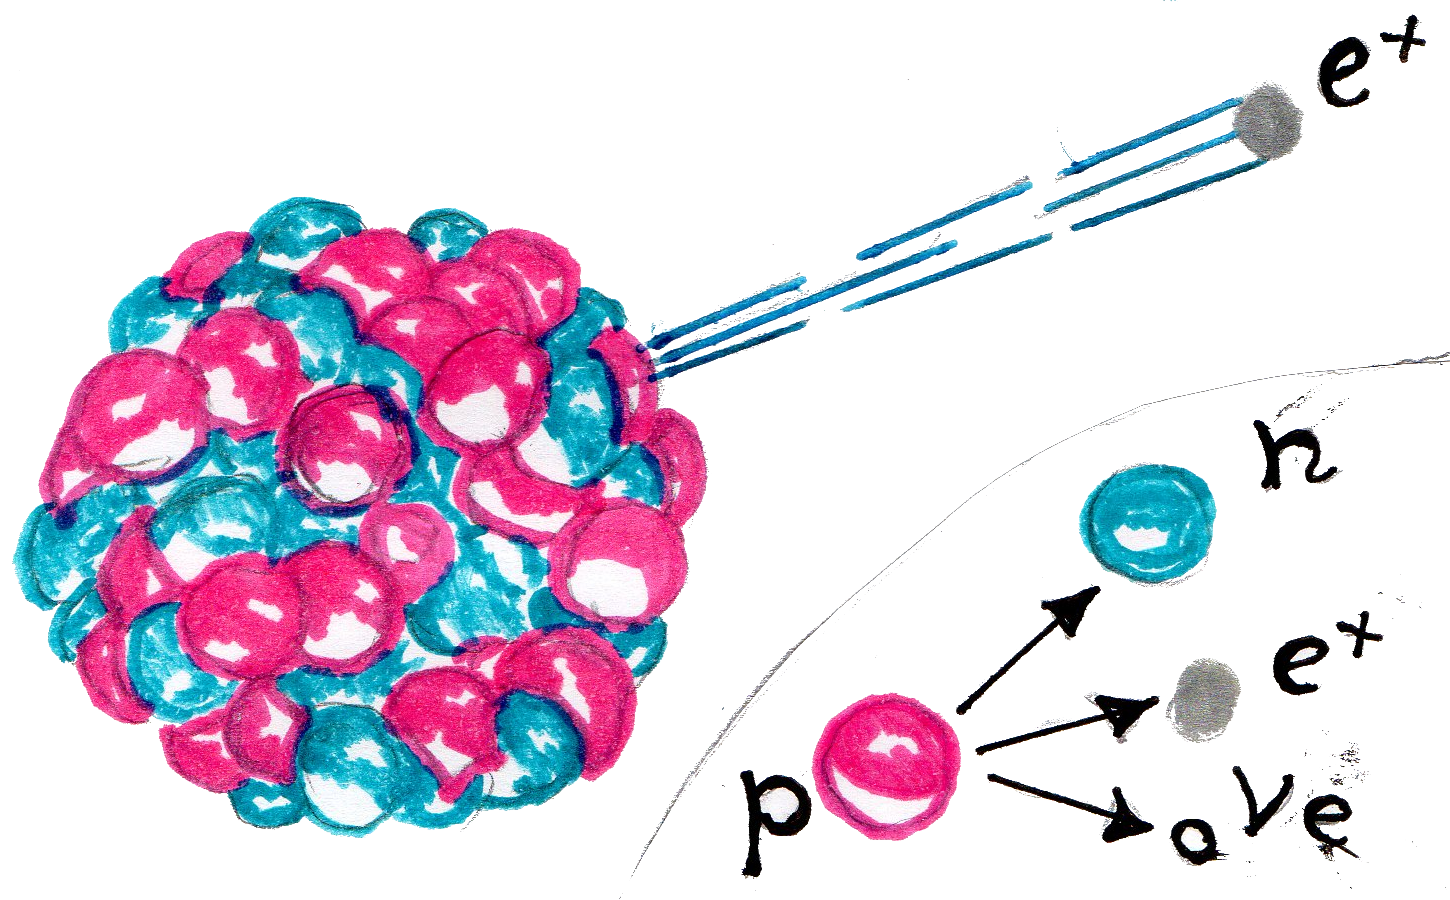
\includegraphics[width=1.0\linewidth]{figures/background_beta_plus_decay.png}
                    
                    \captionsetup{singlelinecheck=false, justification=raggedright}
                    \caption{Graphical example of $\beta+$-decay. Here in the top left of the figure a nucleus can be seen which is unstable as it has an imbalance of protons and neutrons. A positron can be seen exiting the nucleus as a byproduct of $\beta+$-decay converting a proton into a neutron. In the bottom right of the figure a closer example of this can be seen. Here it directly shows a specific proton and the neutron, positron and neutrino which are produced by $\beta+$-decay.} \label{fig:decay_and_annihilation_beta_plus_decay}
                \end{figure}
                
                \begin{figure}
                    \centering
                    
                    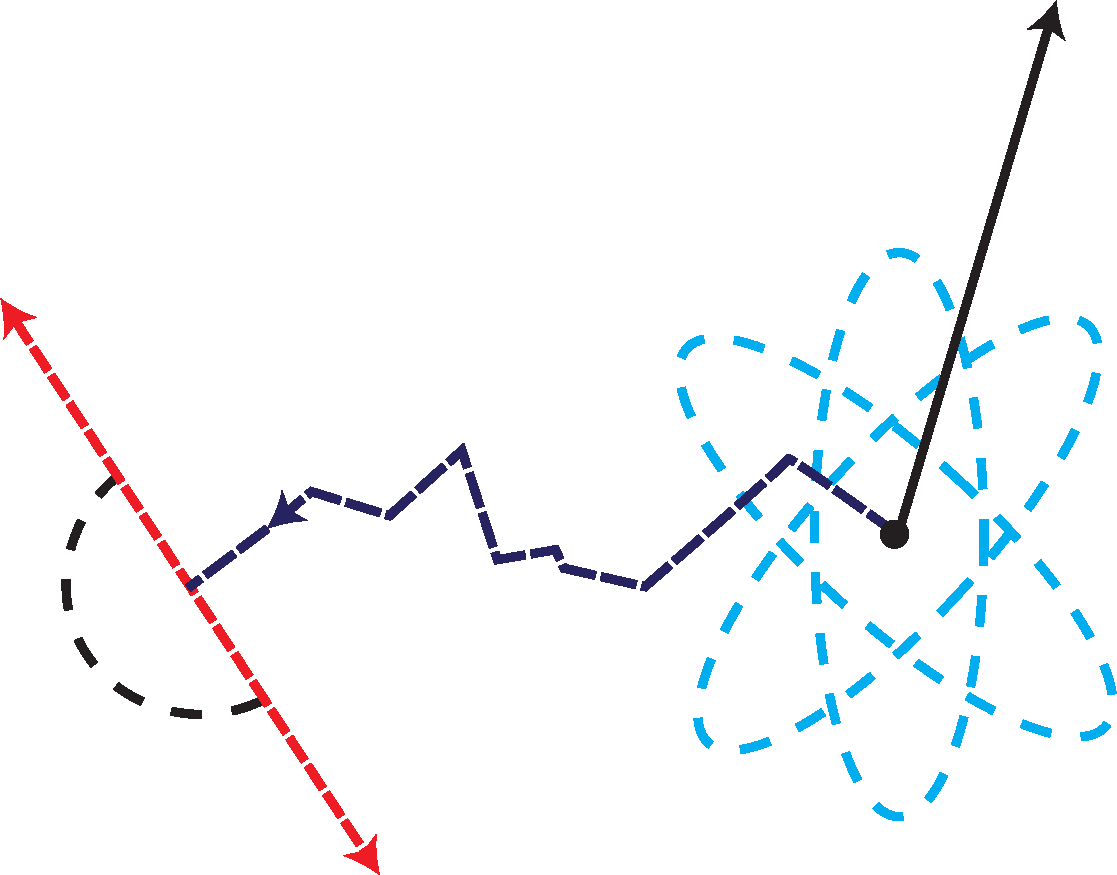
\includegraphics[width=1.0\linewidth]{figures/background_positron_range.png}
                    
                    \captionsetup{singlelinecheck=false, justification=raggedright}
                    \caption{Graphical example of positron range. Here on the right of the figure an atom can be seen travelling with some velocity, a positron is emitted from the nucleus of the atom by $\beta+$-decay. The path that this positron takes can be seen in the centre of the figure represented by a blue line, this path is the positron range. On the left of the figure the annihilation of the positron with an electron occurs and the $\gamma$-photons emitted $\SI{180}{^{\circ}}$ apart are shown.} \label{fig:decay_and_annihilation_positron_range}
                \end{figure}
                
                Radionuclides used in \gls{PET} undergo a type of decay called $\beta+$-decay~\parencite{conti_beta}. This is due to an instability of the radionuclide, because of an imbalance in the number of neutrons to protons in the nucleus. As a consequence, a proton in the atoms nucleus is converted into a neutron subsequently releasing a positron and a neutrino. This can be seen in~\Fref{fig:decay_and_annihilation_beta_plus_decay}. The emitted positron travels with some decreasing velocity, because of sequential collisions, through the body of the patient, for a distance called its positron range.  When the positron will have dissipated its kinetic energy, it will finally collides and annihilates with its antiparticle, the electron. This can be seen in~\Fref{fig:decay_and_annihilation_positron_range}~\parencite{EvansPositronBib}. %KT citation probably not  needed
                
                The annihilation of positron and electron causes the emission of two $511$ \gls{KeV} $\gamma$-photons at $\approx\SI{180}{^{\circ}}$ apart from one another, thus travelling in approximately opposite directions. However, because the positron-electron pair may not be at rest at the moment of their annihilation, the two emitted photons can show a certain degree of non-collinearity, according to the laws of conservation of momentum. This means that the $\gamma$-photons are almost never exactly $\SI{180}{^{\circ}}$ apart~\parencite{scienceofpetspringer}. %KT I'd cut the last sentence. repetition and you don't want to over-elaborate this
                %, because the positron will usually have a small kinetic energy going into the annihilation. This kinetic energy is conserved after the annihilation as a force in a different direction, usually, to that of the force from the annihilation itself.
                
                A \gls{PET} scanner thus does not image, directly, the emission of the positron but, in fact, more closely images the approximate location of its annihilation. %KT move this sentence down a bit %ACW done
            
            \subsubsection{Static and Dynamic Acquisition} \label{sec:static_and_dynamic_acquisition}
                There are two main types of \gls{PET} scan useful for determining separate processes. These types of scans and uses are:
                
                \begin{itemize}
                    \item The first and most common type of \gls{PET} scan is a static \gls{PET} scan~\parencite{Muzi2012QuantitativeImaging}. The patient is scanned only when the injected radiotracer has distributed throughout their body and eventually approximately stabilised. %KT ``perfused'' is wrong. I'd say''distributed''. ``consistent'' sounds weird, so I'd say ``eventually approximately stabilised'' %ACW done, thank you
                    The time elapsed between injection and acquisition depends on the half-life and metabolisation of the radiotracer. For \gls{18F-FDG} about \SI{60}{\minute} is used.
                    
                    \item The second type of \gls{PET} scan is a dynamic scan. The acquisition of data for this scan begins before the radiotracer is injected into the patient. The injection of the radiotracer during the acquisition allows for the kinetics of the radiotracer to be observed and quantified with the use of compartmental modelling~\parencite{Lammertsma2017}. For example, from dynamic \gls{PET} \gls{MPI}: %KT cut the ``direct parametric reconstruction'' here. not used in clinical practice. just say ``dynamic PET MPI''
                    in-vivo studies used in conjunction with radiotracer kinetic modelling enables the quantification of \gls{MBF}, often measured using rubidium-$82$. %Radiotracers such as rubidium $82$ are particularly indicated for dynamic scans given their short half life, seen in~\Fref{sec:decay_and_annihilation}. %KT doesn't have anything to do with halflife but with chemistry (calcium analogue). By the way, the ideal ``tracer'' to measure MBF is (radioactive) water! but that needs cycltron on site etc due to very short half-life. In contrast, Rb82 is produced in a generator. so say ``... MBF, often measured using Rb82.'' %ACW done, thank you, i didnt phrase the half life comment well, i mean that none perfusion or dynamic scans would be difficult with it
                \end{itemize}
            
            \subsubsection{PET Field of View} \label{sec:pet_field_of_view}
                \begin{figure}
                    \centering
                    
                    \includegraphics[width=1.0\linewidth]{figures/background_total_body_pet.png}
                    
                    \captionsetup{singlelinecheck=false, justification=raggedright}
                    \caption{Graphical representation of the difference between a total body \gls{PET} scanner and a standard \gls{PET} scanner. On the left of the figure a total body \gls{PET} scanner can be seen where the rings of detectors completely engulf the patient. However, on the right of the figure a standard \gls{PET} scanner can be seen where the rings of detectors only cover a portion of the patient. On the case on the right of the figure in order to take a scan over the entire body either individual acquisitions will be needed and concatenated or the bed would have to move while the acquisition was ongoing.} \label{fig:pet_fov_total_body_pet}
                \end{figure}
                
                The \gls{FOV} of the scanner is the area in which $\gamma$-photons can be detected. Current clinical \gls{PET} scanners, usually, have a cylindrical \gls{FOV} with a length of between \SI{15.0}{\centi\metre} and \SI{25.0}{\centi\metre} and a diameter of between \SI{50.0}{\centi\metre} and \SI{70.0}{\centi\metre}~\parencite{Pan2019}.
                
                There are multiple ways to acquire data over more than the axial length of scanner, three of these methods are:
                
                \begin{itemize}
                    \item The most simple and widely used method is to take acquisitions over multiple bed positions and concatenate them.
                    
                    \item A method available on some  standard axial length scanners is; to continually move the bed through the rings of the scanner while acquiring data. This is advantageous as it is more comfortable for the patent and provides potentially less movement of the patient. %KT both these advantages can be done with the above step-and-shoot as well. I guess the advantages are patient comfort and potentially less moveemnt of the patient %ACW done
                    A disadvantage of this though is that it introduces another source of motion to the acquisition from moving the bed. This makes standard \gls{MC} much more difficult.
                    
                    \item Alternatively, total body \gls{PET} scanners are becoming more viable for research. %KT let's remove the ``high potential for  clinical applicatoin''. as you note below,price prevents this %ACW done
                    Total body \gls{PET} scanners have an axial \gls{FOV} which contains most of the patients body making multiple acquisitions less necessary while also increasing the sensitivity of the scanner, this can be seen in~\Fref{fig:pet_fov_total_body_pet}~\parencite{Cherry2018}. However, the increased price and size constitute a limitation.
                \end{itemize}
            
            \subsubsection{Attenuation} \label{sec:attenuation}
                \begin{figure}
                    \centering
                    
                    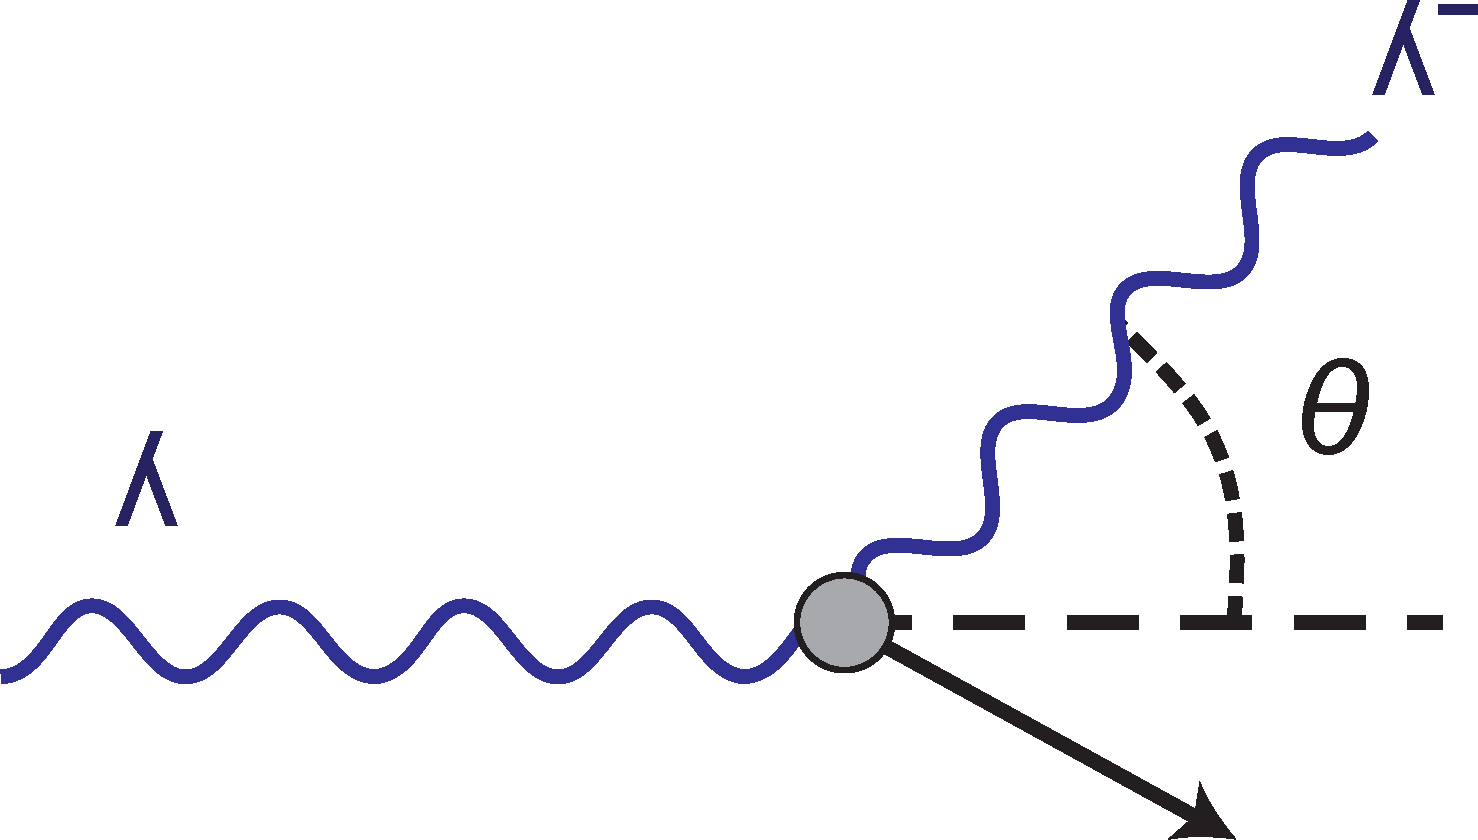
\includegraphics[width=1.0\linewidth]{figures/background_scatter.png}
                    
                    \captionsetup{singlelinecheck=false, justification=raggedright}
                    \caption{Graphical representation of a $\gamma$-photon scattering off of a particle. The $\gamma$-photon can be seen entering the figure on the left hand side before scattering off of a particle in the centre of the figure by an angle $\theta$ and exiting the figure on the top right hand corner. The electron exits the scatter event with some velocity represented by the arrow towards the bottom right. 
                    } \label{fig:attenuation_scatter}
                \end{figure}
                
                %KT ``amount of counts'' is not correct. it's a process, or effect, not a number
                %ACW done
                %KT ``who quite literally...'' this doesn't read quite correct.I'd remove that part of the sentence
                %ACW done
                Attenuation is the process or effect through which counts are lost from annihilation to detection by the scanner while the photons are traversing through the body of the patient. Attenuation can amount to a loss of up to \SI{95.0}{\percent} of the total initial signal and can cause increased issues in larger bariatric patients~\parencite{petspringer}~\parencite{Essential2012}. %KT''book'' citation looks strange. missing space in the bibtex? also the guiberteau initials seem strange %ACW done
                
                There are three main ways through which the photon signal can be lost~\parencite{scienceofpetspringer}, these are in ascending order of magnitude:
                
                \begin{itemize}
                    %KT this isn't a signal loss. I'd cut it (as it doesnt happen in PET)
                    %ACW done
                    %\item Pair production can be thought of as the inverse process compared to annihilation (as discussed above). This is where a subatomic particle and its antiparticle, such as a electron and a positron, are created from a fundamental particle, such as a photon, usually in close proximity to an atomic nucleus~\parencite{Hubbell2006Electron-positronOverview}. However, because of conservation of energy a photon would need to be of at least $1.022$ \gls{MeV} which is not generally possible for photons created through electron positron annihilation.
                    
                    \item Rayleigh scattering is the elastic scattering of photons, without loss of significant energy, by particles which are much smaller than the wavelength of the photon. A common example of Rayleigh scattering is the scattering of sunlight in the atmosphere which causes the blue colour of the sky during the day and the red colour of the sky at sunset. Because the wavelength of $\gamma$-photons are comparably small, compared to most particles, the probability of Rayleigh scattering occurring is negligible and thus it is normally ignored in \gls{PET}.
                    
                    \item Absorption through the photoelectric effect is the process through which a high energy $\gamma$-photon hits and transfers its energy to a material causing the emission of a lower energy electron. The likelihood of the photoelectric effect is inversely proportional to the cube of the photon energy; it also increases as the atomic number of the attenuating material increases. In the matter of the patient the photoelectric effect is most prevalent at photon energies below $100$ \gls{KeV} and as such the probability of the photoelectric effect occurring for the \gls{PET} $\gamma$-photons is minimal~\parencite{petspringer}. %KT ``here'' say instead ``for the PET gamma photons'' or so. phtoelectirc effect does occur for CT X-rays %ACW done
                    Attenuation through the photoelectric effect occurs mostly in the detectors of the scanner (it's the principle underlying the function of scintillator crystals).
                    
                    \item Compton scattering comprises the majority of interactions between the photon and matter in \gls{PET}, it occurs where the photon interacts with an electron in a close by atom. The recoiling electron causes the photon to be deflected along another path transferring energy from photon to electron, this can be seen in~\Fref{fig:attenuation_scatter}. Compton scattering is also known as incoherent scattering. The probability of Compton scattering is indirectly proportional to the energy of the photon~\parencite{petspringer}.
                \end{itemize}
                
                The relationship between the attenuation of the signal and the material through which it is travelling is given by the Beer-Lambert law. Given $I_0$ incident photons travelling across a path $D$, the number of non-scattered photons $\rmI_{\rmD}$ is given by: %KT given all of the above,I recommend to say ``the numberof  non-scattered photons...'' %ACW done
                 
                \begin{equation} \label{sec:eq:beer_lambert_law}
                    \rmI_{\rmD} := \rmI_{0} \cdot \exp\Bigg(\int_{\rmD} - \mu_E(r)\rmd r \Bigg) %KT why := ? %ACW done, because i wanted to be consistent
                \end{equation}

                \noindent where $\mu_E(r)$ is the attenuation coefficient of the media crossed by photons of energy $E$.
        
        \subsection{Data acquisition} \label{sec:data_acquisition}
            % write a general intro on the scanner structure, and the type of events you detect (true scatter randoms etc)
            
            \begin{figure}
                \centering
                
                
\includegraphics[width=1.0\linewidth]{figures/background_coincidence.png}
                
                \captionsetup{singlelinecheck=false, justification=raggedright}
                \caption{Graphical representation of the different types of coincidences possible in \gls{PET}. On the left of the figure a true coincidence can be seen, this is where the $\gamma$-photons from one annihilation are both detected without scattering. In the middle of the figure a scattered coincidence can be seen, this is where the $\gamma$-photons from one annihilation are both detected, however in this case one of them has scattered. On the right of the figure a random coincidence can be seen, this is where the $\gamma$-photons from two unrelated annihilations are detected.} \label{fig:data_acquisition_coincidence}
            \end{figure}
            
            As discussed in~\Fref{sec:pet_field_of_view}, the structure of a \gls{PET} scanner is that of concentric rings of detectors offset along a central axis. These rings detect each incident photon and attempt to temporally and spatially link opposing photons along a \gls{LOR} through the scanner. A \gls{LOR} being a line through the \gls{FOV} of the scanner linking two detectors. The methods through which the scanner attempts to %detect incident photons and then 
            link relative photons together will be discussed in the following %~\Fref{sec:photon_detection} and
            ~\Fref{sec:coincidence_processing}.
            
            Because of the photons interaction in matter shown in~\Fref{sec:attenuation}, there are four different types of event or coincidences that can be detected by the scanner, these are:
            
            \begin{itemize}
                \item Firstly, the coincidences that originate from the same annihilation event and pass through the body of the patient to the detector without being scattered or attenuated. These coincidences are called true coincidences as they approximately accurately reflect the position of the originating annihilation and thus the underlying activity distribution.
                
                \item Secondly, there are coincidences which may have originated from the same annihilation event but, from which one or more of the incident photons has undergone Compton scattering before detection. These coincidences are called scattered coincidences. Scattered coincidences can attempt to be corrected for if an accurate \gls{Mu-Map} is given, the density of the matter through which the photons must have travelled indicate the likelihood of scattering.
                
                \item Thirdly, there are coincidences where the \gls{LOR} is determined from two photons from two distinct annihilation events, thus the \gls{LOR} does not reflect an actual annihilation in reality. This could occur because one or more of the photons, from the original pair of photons, may have been attenuated or scattered so that it does not arrive at the detector within a reasonable time of its photon pair or that its \gls{LOR} doesn't go through one of the detectors. %KT  much more likely is that its LOR actually doesn't go through one of the detectors! (it's a 3D process of course) %ACW done
                These are called random coincidences. Random coincidences can be corrected for if acquisition data of this background level of the scan exists.
                
                \item Fourthly, there could be a situation where three or more photons are detected within close temporal proximity to one another. Because of the close time of detection, in this case it is not possible to determine which photons reflect an actual annihilation and which are random coincidences. These coincidences are called multiple coincidences. In normal procedures this is rare. %KT I recommend say that this is in normal procedures  rare. Otherwise an obvious viva question would be what people would do with them (as they're not in your equation below) %ACW done
            \end{itemize}
            
            An example of some of the types of coincidences from above can be seen in~\Fref{fig:data_acquisition_coincidence}.
            
            The total prompts detected during a \gls{PET} acquisition $P$ can be expressed as:
            
            \begin{equation}
                P := T + S + R
            \end{equation}
            
            \noindent where $T$ is the number of true coincidences, $S$ is the number of scattered coincidences and $R$ is the number of random coincidences. %Thus the usual total sum of scattered and random coincidences when compared to true coincidences is a ratio of $2$ to $1$. %KT this last sentence is incorrect. depends on count-rate, amount of scatter etc etc. Delete it %ACW done
            
%            \subsubsection{2D and 3D Acquisition} \label{sec:2d_and_3d_acquisition}
                %KT the 2D stuff reads as if in 2D PET there were collimators between all detectors, but in fact they were only between rings.
                %I highly recommend cutting this subsubsection. Detail not relevant to your work.
                %ACW depressingly done
%                \begin{figure}
%                    \centering
                    
%                    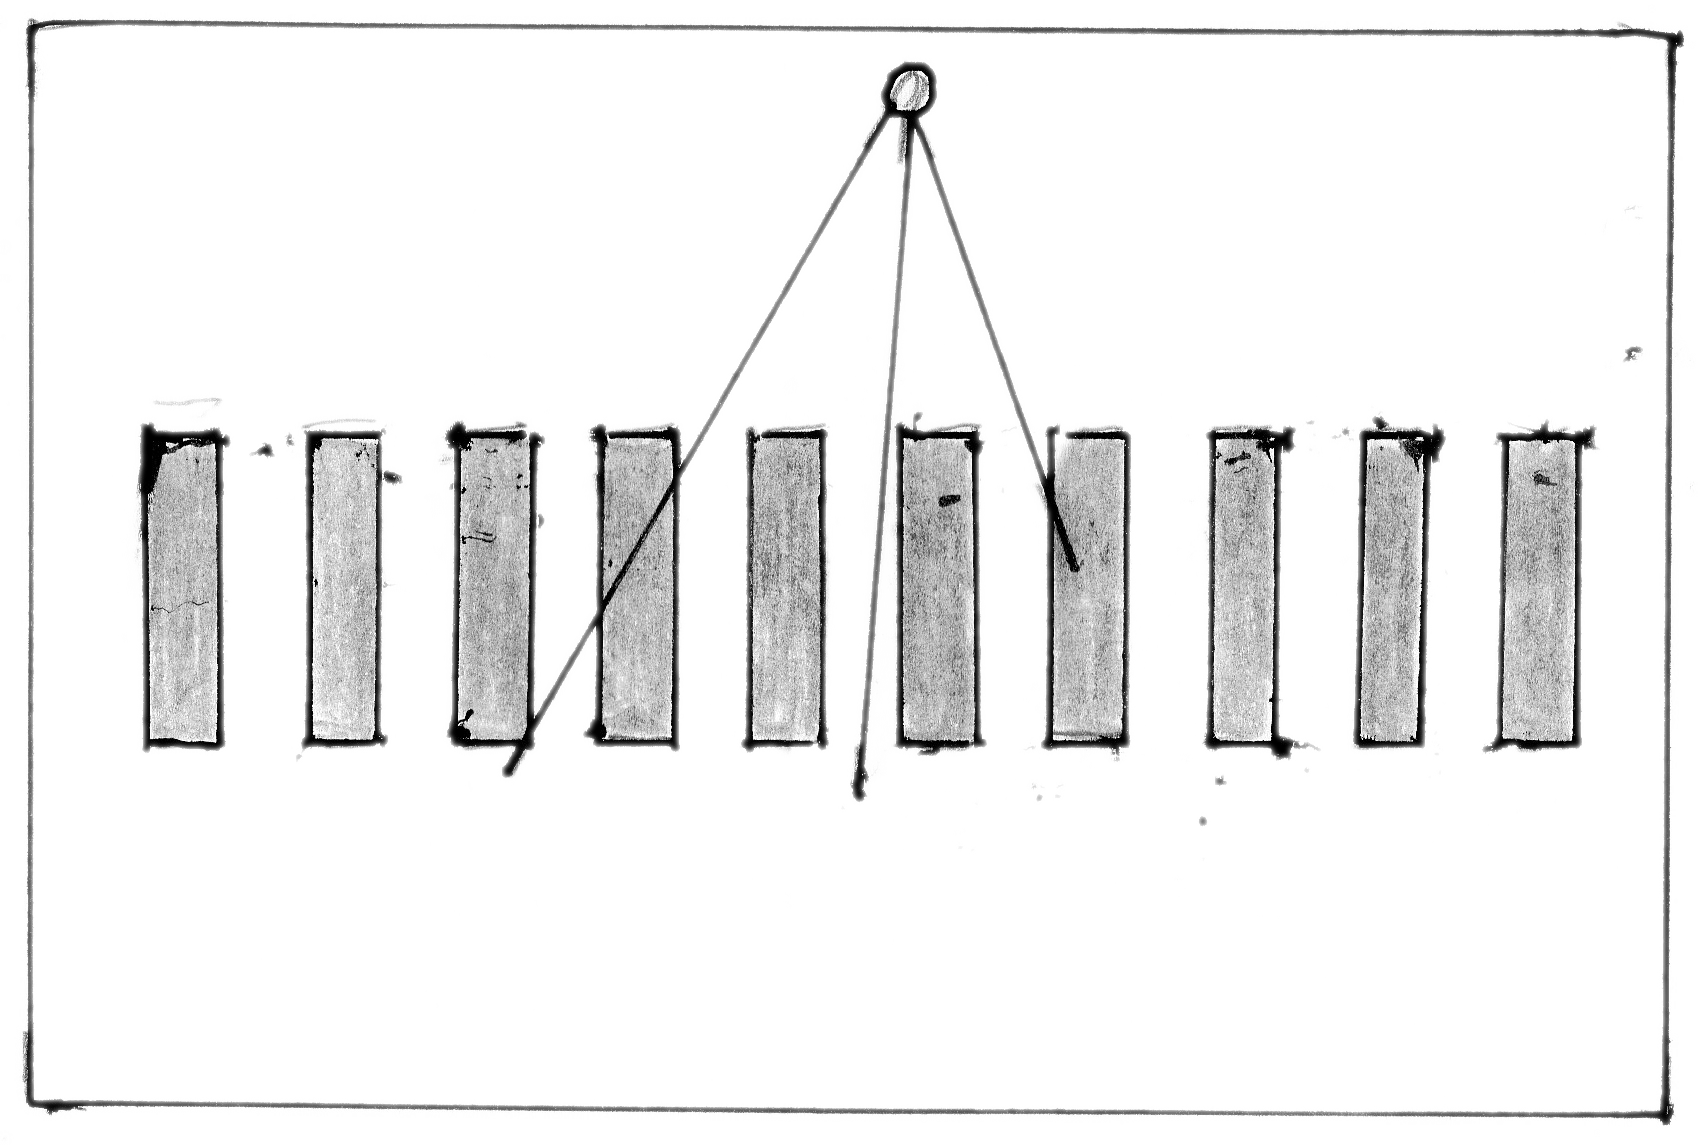
\includegraphics[width=1.0\linewidth]{figures/background_septa.png}
                    
%                    \captionsetup{singlelinecheck=false, justification=raggedright}
%                    \caption{Graphical representation of the cross section of the septa used for collimation in \gls{2D} \gls{PET} acquisitions. In this figure a point can be shown casting paths into the slits of the septa, as can be seen the paths from the point can only pass through the slits of the septa in positions where the angle of the line with respect the the walls of the septa is acute.} \label{fig:2d_and_3d_acquisition_septa}
%                \end{figure}
                
%                There are two different methods used in \gls{PET} to determine or constrain to be certain of the spatial position or angle of the \gls{LOR} along the axis of the scanner, these are:
                
%                \begin{itemize}
%                    \item The method which was used for a long time in other applications (such as \gls{SPECT}) and until recently in \gls{PET} was; to place a block of, usually, tungsten metal (for its photon absorbing properties) in front of all of the detectors, this block is called s septa, this can be seen in~\Fref{fig:2d_and_3d_acquisition_septa}. The septa has very small slits cut into it which would only allow photons to pass through which entered the slits at an acute angle. Thus the septa constrains the photons to being almost perpendicular to the detector (on axis) and as such each detector only receives signal from annihilations that occur within its ring. This process is called collimation and the subsequent acquisition is called a \gls{2D} acquisition, \gls{2D} not because it results in a single image but because it is comprised of distinct \gls{2D} projections.
                    
%                    \item The more modern method is to simply remove the septa from the scanner and to record coincidences between all rings. This is significantly more computationally expensive than a \gls{2D} acquisition but it also increases the sensitivity of the scanner meaning that scanning times can be reduced. Because this method produces projections between all rings it is known as a \gls{3D} acquisition~\parencite{Schmitz2013}~\parencite{Bailey1998ExperienceTomographs}.
%                \end{itemize}
            
%            \subsubsection{Photon Detection} \label{sec:photon_detection}
                %KT I did not read this. Far far too much detail for your thesis. I highly recommend commenting it out
                %ACW depressingly done
%                \begin{figure}
%                    \centering
                    
%                    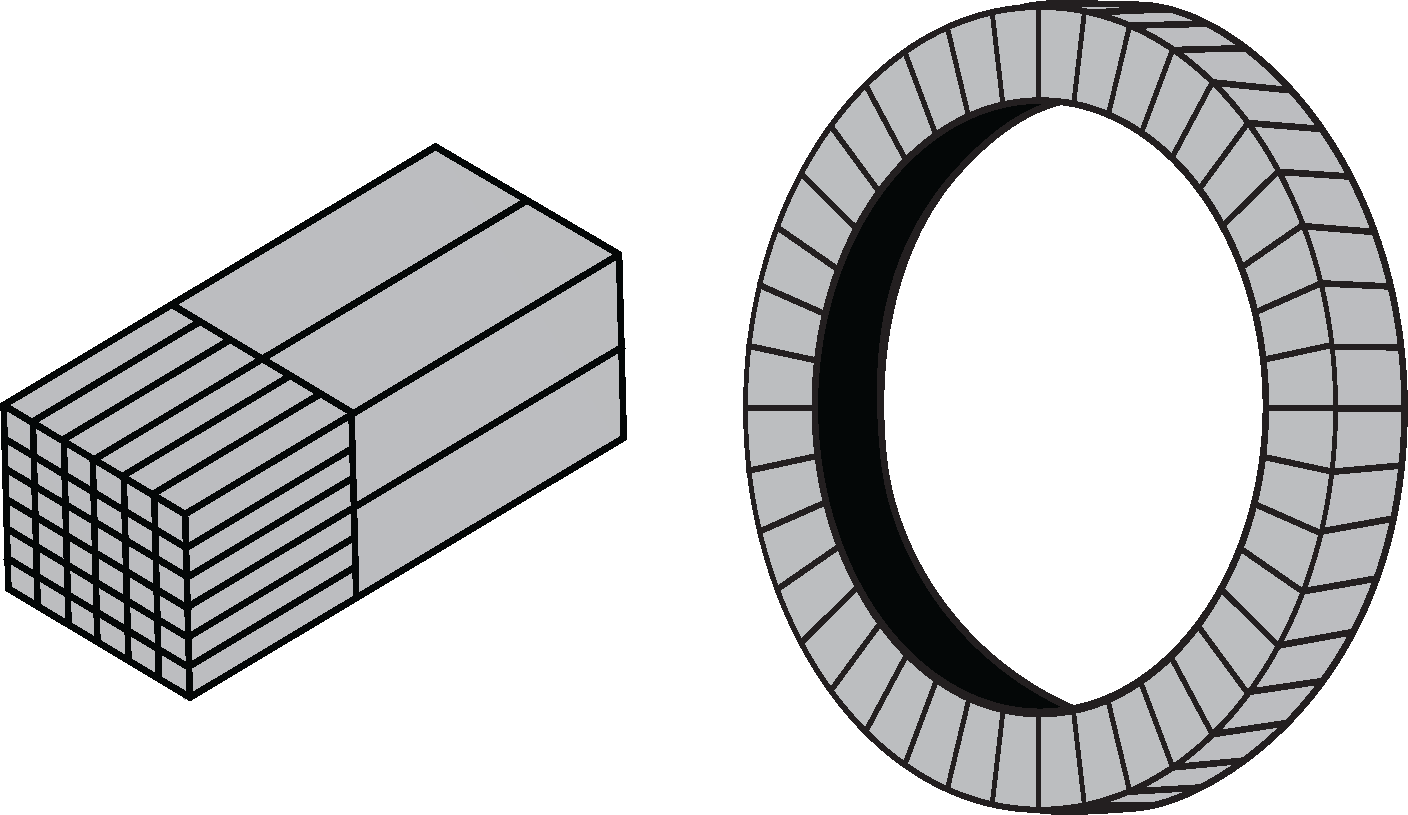
\includegraphics[width=1.0\linewidth]{figures/background_detector.png}
                    
%                    \captionsetup{singlelinecheck=false, justification=raggedright}
%                    \caption{Graphical representation of the block detector structure of the scintillator crystal and the photodetector (with multiple scintillator crystals per photodetector), on the left of the figure, and an example of how these block detectors would be combined to construct a ring of a \gls{PET} scanner, on the right of this figure.} \label{fig:photon_detection_detector}
%                \end{figure}
                
%                \begin{figure}
%                    \centering
                    
%                    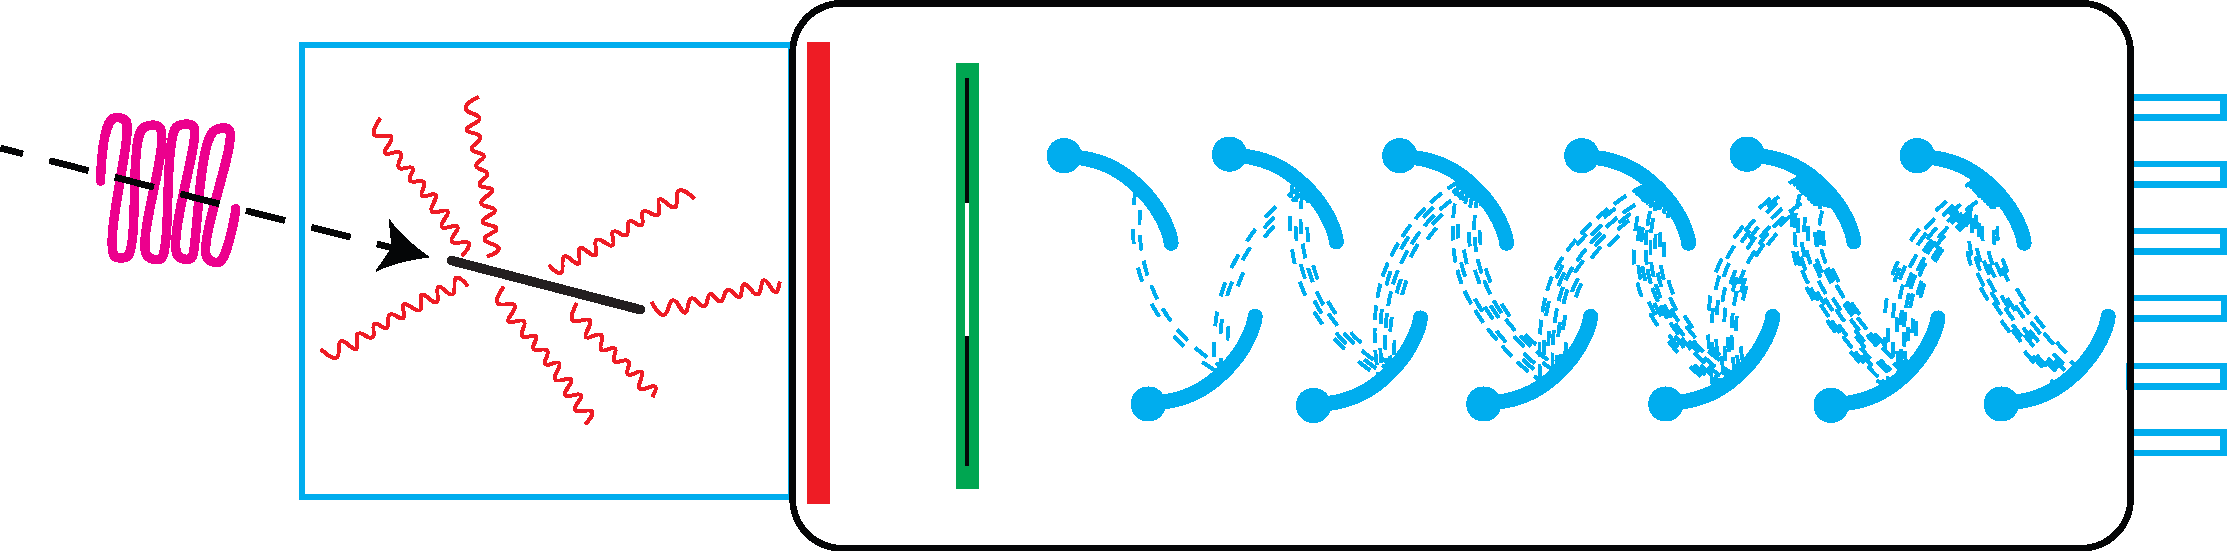
\includegraphics[width=1.0\linewidth]{figures/background_photomultiplier.png}
                    
%                    \captionsetup{singlelinecheck=false, justification=raggedright}
%                    \caption{Graphical representation of a scintillator crystal coupled to a \gls{PMT}. On the left of this figure a photon can be seen impinging upon the scintillator crystal and then being attenuated by the photoelectric effect at some depth. The electrons produced by this can then be seen, in the centre of this figure, interacting with the photocathode before being focused onto the first dynode. On the right of this figure, a naive representation, the amplification of the electrons can be seen by subsequent dynodes.} \label{fig:photon_detection_photomultiplier}
%                \end{figure}
                
%                PET detectors consist of two main components; a scintillator crystal, which, partially because of the photoelectric effect, when exposed to ionising radiation produces visible light through luminescence, and a photodetector or photomultiplier which amplifies the intensity of an input light similarly to how a vacuum tube or a transistor would amplify an electrical signal. These can be seen in~\Fref{fig:photon_detection_detector}.
                
%                For use in \gls{PET} the following properties are desirable for a scintillator crystal:
                
%                \begin{itemize}
%                    \item Firstly, the crystal should have a high stopping power. This means that the photon does not travel a great distance into the crystal before it undergoes attenuation by the photoelectric effect. Usually the higher the density of the scintillator crystal the greater the stopping power~\parencite{Derenzo2003TheScintillator}.
                    
%                    \item Secondly, for each incident photon the scintillator should have a high light output. This not only means that the work photomultiplier will have to amplify the output less but it also means that discriminating between scattered and unscattered photons will be easier as the discrepancy between the output intensity of the two will be greater.

%                    \item Thirdly, the scintillator should return to a state where it can luminesce again rapidly after each incident photon. This means that more photons can be detected over time and that the exact moment a photon is attenuated can be better measured.
                    
%                    \item Finally, a scintillator crystal should not be hygroscopic. To be hygroscopic means that something has a tendency to absorb water.
%                \end{itemize}
                
%                The first \gls{PET} scanners used \gls{NaI} scintillator crystals before moving to \gls{BGO} and then to \gls{LSO} and \gls{LYSO}. Each new generation of scintillator crystals provided a different balance of the above characteristics. \gls{LSO} and \gls{LYSO} have the best combination of efficiency and time resolution while not being hygroscopic~\parencite{BGOCherenkovBib}~\parencite{ScintilatorsBib}~\parencite{Mao2013CrystalCrystals}.
                
%                There are three main types of photodetector or photomultiplier, these are:
                
%                \begin{itemize}
%                    \item The first kind of photodetector to be used in \gls{PET} was the \gls{PMT}, this device functions using an initial photocathode and a focusing electrode which takes the output from the scintillator and directs it towards a chain of dynodes. Dynodes are an intermediate electrode which when struck by a photoelectron emit more photoelectrons at a more positive electrical potential through secondary emission. Each subsequent dynode is a a higher potential and emits more photoelectrons than the last causing the input signal to be amplified, this can be seen in~\Fref{fig:photon_detection_photomultiplier}. Some disadvantages of \glss{PMT} are that they are relatively bulky, are effected by a magnetic field and have a relatively low efficiency at approximately \SI{25.0}{\percent}~\parencite{petspringer}~\parencite{SiPmBib}.
                    
%                    \item To attempt to combat the low efficiency mentioned above the \gls{APD} was developed, this device utilises a semiconductor where there is a junction between positive and negative type silicone, this is similar to a traditional diode. This allows for efficiencies approaching \SI{85.0}{\percent}, they are much smaller than \glss{PMT} and are safe to be used in a magnetic field. However, this also comes with the drawbacks that \glss{APD} produces so much heat that it requires an active cooling system and exhibits worse timing characteristics than \glss{PMT}~\parencite{AvalanchePhotodiodeBib}. \glss{APD} are the choice of many modern \gls{PET}/\gls{CT} scanners~\parencite{Vandendriessche2019}.
                    
%                    \item A further development on \glss{APD} gave \glss{SiPM} and \glss{SSPM}. These devices combine the benefits of both \glss{PMT} and \glss{APD} in that they have a high efficiency, small size, are safe to be used in a magnetic field and have good timing characteristic. \glss{SiPM} and \glss{SSPM} are becoming the new default photodetectors in \gls{GE} scanners~\parencite{SiPmBib}.
%                \end{itemize}
            
            \subsubsection{Coincidence Processing} \label{sec:coincidence_processing}
                % write stuff about coincidence processing , give some info on TOF (or separate section for it, i don't know)
                
                \begin{figure}
                    \centering
                    
                    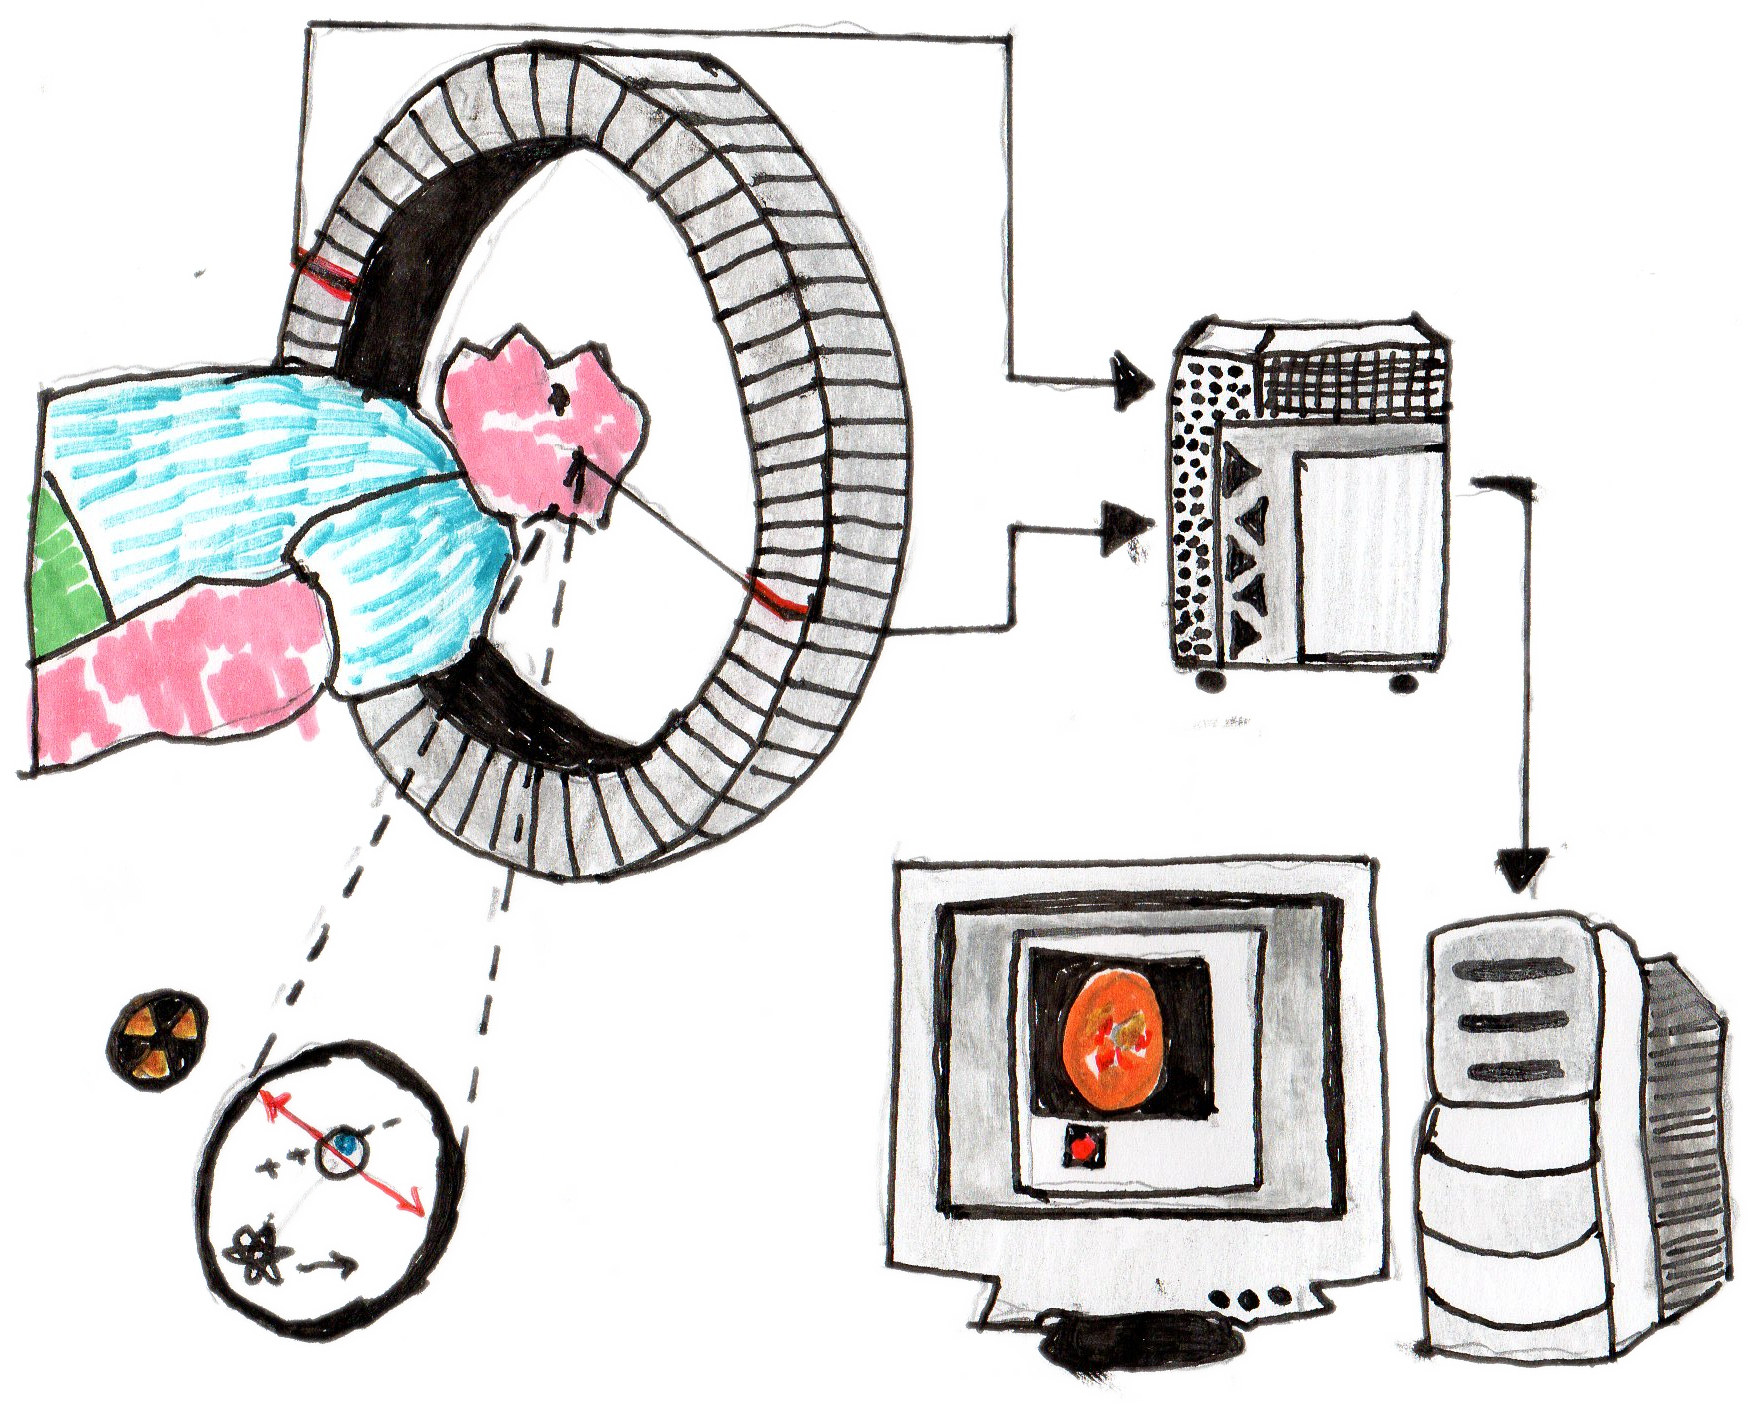
\includegraphics[width=1.0\linewidth]{figures/background_coincidence_processing.png}
                    
                    \captionsetup{singlelinecheck=false, justification=raggedright}
                    \caption{Graphical representation of the workflow from annihilation, to physical detection by the scanner, to then coincidence processing by the electronics of the scanner, before finally displaying some output to the user.} \label{fig:coincidence_processing_coincidence_processing}
                \end{figure}

                %KT first sentence sounds a bit weird. what does an LOR have to do with this? I'd shorten it.
                %ACW done
                %In order for a \gls{LOR} to be determined, the annihilation from which pairs of detected photons come from must be determined, in other words, they must be paired together in some way, as briefly mentioned above in~\Fref{sec:data_acquisition}.
                In order to form coincidences, the incident photons must be paired together to an annihilation event. First, before forming coincidences, the photons are filtered by selecting ones which only fall within an energy window of the scanner, for the \gls{GE} Discovery $690$/$710$ \gls{PET}/\gls{CT} this energy window falls approximately between $425$ and $600$ \gls{KeV}~\parencite{Bettinardi2011}. Additionally, to attempt to determine temporally if two detected photons belong to the same annihilation event a coincidence window is used. If the events arrive more than the time of the coincidence window apart then they are determined to be unrelated. A standard coincidence window size would be about \SI{5.0}{\nano\second}. A naive representation of the workflow for coincidence processing can be seen in~\Fref{fig:coincidence_processing_coincidence_processing}.
            
            \subsubsection{Time of Flight PET} \label{sec:time_of_flight_pet}
                \begin{figure}
                    \centering
                    
                    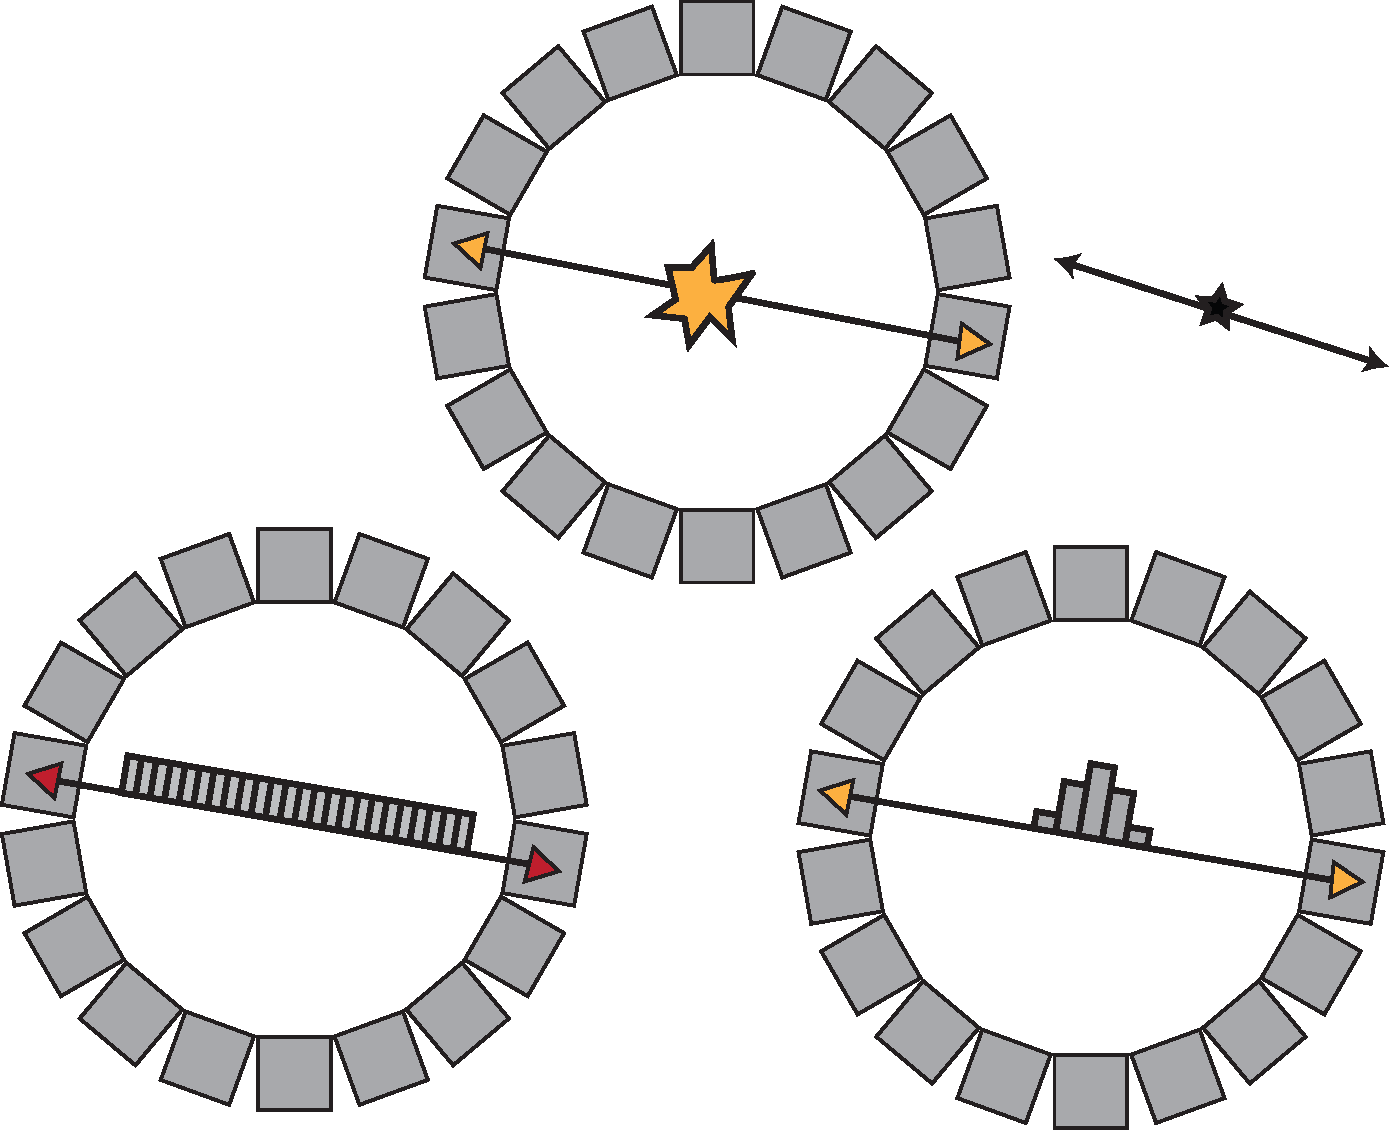
\includegraphics[width=1.0\linewidth]{figures/background_tof.png}
                    
                    \captionsetup{singlelinecheck=false, justification=raggedright}
                    \caption{Graphical representation of the concept of \gls{TOF}. The top middle of this figure shows the position where a hypothetical annihilation has occurred, plus the $\gamma$-photos from this annihilation which have then gone on to be detected by the scanner. The bottom left of this figure shows a traditional \gls{NTOF} acquisition where the probability of the position of the annihilation along the \gls{LOR} is constant. The bottom right of this figure shows a \gls{TOF} acquisition where the probability of the position of the annihilation along the \gls{LOR} can be approximated with a Gaussian based upon the difference in arrival time of both photons.} \label{fig:time_of_flight_pet_tof}
                \end{figure}
                
                \begin{figure}
                    \centering
                    
                    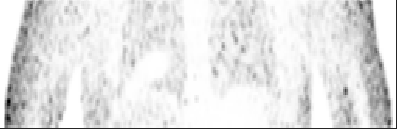
\includegraphics[width=1.0\linewidth]{figures/background_non_tof_example.png}
                    
                    \captionsetup{singlelinecheck=false, justification=raggedright}
                    \caption{Example of some \gls{NAC} \gls{NTOF} data, with noise, with no motion, randoms or scatters, of the thorax with a spherical lesion in the lungs. Coronal view.} \label{fig:time_of_flight_pet_non_tof_example}
                \end{figure}
                
                \begin{figure}
                    \centering
                    
                    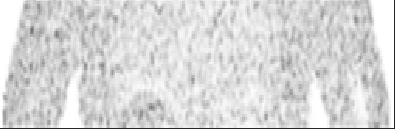
\includegraphics[width=1.0\linewidth]{figures/background_tof_example.png}
                    
                    \captionsetup{singlelinecheck=false, justification=raggedright}
                    \caption{Example of some \gls{NAC} \gls{TOF} data, with noise, with no motion, randoms or scatters, of the thorax with a spherical lesion in the lungs. Coronal view.} \label{fig:time_of_flight_pet_tof_example}
                \end{figure}
                
                As stated above in~\Fref{sec:coincidence_processing}, in order for the coincidence window based method to determine which specific detected photons represent \glss{LOR}, the scanner must be able to asses the difference in arrival time of each photon. %Because of this the scanner must record the absolute time at which it detects each incident photon. %KT delete previous sentence. it isn't really  necessary and essentially irrelevant anyway %ACW done
                It had been hypothesised for some time (since the $1960$s) that given the speed of light and the difference in arrival time at each detector, for each photon that makes a specific \gls{LOR}, then it should be possible to approximately calculate the position upon the \gls{LOR} at which a given annihilation occurred. %, known as \gls{TOF}. %KT ``know as TOF'' doesn't flow with the rest of the sentence %ACW done
                This can be seen in~\Fref{fig:time_of_flight_pet_tof}~\parencite{Surti2015}~\parencite{TOFPhotodetectorsBib}.
                
                The reason for the uncertainty of the position along the \gls{LOR} is because of the relatively course timing resolution of each given scanner. Generally modern \gls{PET}/\gls{CT} scanners have a timing resolution ranging between \SI{200.0}{\pico\second} and \SI{600.0}{\pico\second}, which represents an approximate spatial uncertainty of between \SI{30.0}{\milli\metre} and \SI{90.0}{\milli\metre}. %KT I think you forgot to divide by 2 %ACW done
                The uncertainty within these \gls{TOF} bins is usually modelled using a Gaussian distribution centred around the estimated position of annihilation by the scanner, with standard deviation dependent on the time resolution.
                
                %KT cut next paragraph. too much detail for you
                %ACW depressingly done
                %The timing resolution of the scanner is mainly dictated by the timing properties of both the scintillation crystal and the photodetector used. For the scintillation crystal, almost ubiquitously \gls{LSO} and \gls{LYSO} are used in modern \gls{PET} scanners which utilise \gls{TOF}. This is because they are the only scintillation crystals where they stop the photon and return to their base state post luminescence in a suitable time such that the time of arrival can be determined to any useful degree~\parencite{TOFLSOBib}. For the photodetector, though \glss{PMT} possessed suitable timing properties to be used for \gls{TOF} now \glss{SiPM} and \glss{SSPM} are surpassing \glss{PMT} both in their timing properties and because they are not affected by magnetic fields and such can be used in both \gls{PET}/\gls{CT} as well as \gls{PET}/\gls{MR} scanners.
                
                Currently, \gls{TOF} is a focus for research because of the drastic improvements that it can have on the \gls{SNR}~\parencite{Lecoq2017}~\parencite{Cates2018}. %\gls{TOF} has such an impact on the resolution and reconstruction of \gls{PET} that it is used as a pseudo attenuation correction technique outside of the \gls{FOV} of the \gls{MR} in some \gls{PET}/\gls{MR} systems, such as the \gls{GE} Signa~\parencite{Pan2019}. %KT I'd cut the previous sentence. This is  far more complicated than this (needs MLAA etc) %ACW done
                An example of some \gls{NAC} \gls{NTOF} and \gls{NAC} \gls{TOF} data can be seen in~\Fref{fig:time_of_flight_pet_non_tof_example} and~\Fref{fig:time_of_flight_pet_tof_example} respectively, notice the difference in distribution of counts in the centre of the thorax and lungs.
                
                The current (as of $2021$) \gls{PET}/\gls{CT} scanner with the highest \gls{TOF} resolution which is commercially available is the Siemens Vision with an approximate \gls{FWHM} of \SI{210.0}{\pico\second} or \SI{31.5}{\milli\metre}~\parencite{VanSluis2019}. The \gls{PET}/\gls{MR} scanner with the highest \gls{TOF} resolution which is commercially available is the \gls{GE} Signa with an approximate \gls{FWHM} that is sub \SI{400.0}{\pico\second} or \SI{60.0}{\milli\metre}~\parencite{SIGNA}~\parencite{Hsu2017StudiesSystem}~\parencite{SIGNA}~\parencite{Caribe2019NEMAIsotopes}. %KT again factor 2in the mm %ACW done
            
            \subsubsection{Data Output} \label{sec:data_output}
                \begin{figure}
                    \centering
                    
                    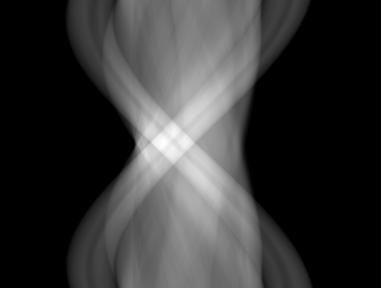
\includegraphics[width=1.0\linewidth]{figures/background_sinogram_data_example.png}
                    
                    \captionsetup{singlelinecheck=false, justification=raggedright}
                    \caption{Example of some simulated sinogram data, with no motion, noise, randoms or scatters, of the thorax with a spherical lesion in one of the lung.} \label{fig:data_output_sinogram_data_example}
                \end{figure}
                
                \begin{figure}
                    \centering
                    
                    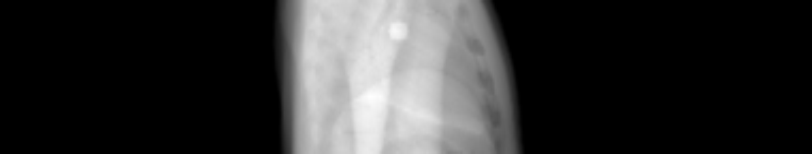
\includegraphics[width=1.0\linewidth]{figures/background_viewgram_data_example.png}
                    
                    \captionsetup{singlelinecheck=false, justification=raggedright}
                    \caption{Example of some simulated viewgram data, with no motion, noise, randoms or scatters, of the thorax with a spherical lesion in one of the lung.} \label{fig:data_output_viewgram_data_example} %KT fine, but it hardly shows what it's a sinogram (as you used a viewgram). maybe show both? %ACW done
                \end{figure}
                
                The output from a \gls{PET} scanner must be stored in a %universally understood
                file format in order to be of any use. %KT not true (in theory, but also not in practice. As long as the manfacturer can read it, they're fine...) %ACW done
                This file format will usually contain information related to the prompts from the acquisition, discussed above in~\Fref{sec:data_acquisition}. Each prompt stored represents a \gls{LOR} connecting the centre of two detectors. %KT probably first time you define LOR, while used multiple times above %ACW done
                Where \gls{TOF} information is available it is stored as an extra dimension in this file. This file can then be taken and reconstructed in order to estimate the original distribution of the radiotracer, this will be discussed later in~\Fref{sec:pet_image_reconstruction}.
                
                There are two main formats in which this information is stored from the scanner:
                
                \begin{itemize}
                    \item The most common way, that is used in clinical practise, is a format called a sinogram. During acquisition, if a sinogram output is specified, then the coincidences detected by the scanner are binned into a histogram which represents their plane orthogonal to the scanner, their orientation angle, their average axial location and their distance from the centre of the gantry. \gls{TOF} can be added as an additional dimension if it is used. %KT and TOF... %ACW done
                    If a single point source were imaged it would produce a sinusoid when binned into a sinogram, hence the name. An example of sinogram (where the \gls{LOR} are in a given transaxial plane) and viewgram (where the \gls{LOR} are along a given view, parallel to each other) data, with no noise, can be seen in~\Fref{fig:data_output_sinogram_data_example} and~\Fref{fig:data_output_viewgram_data_example} respectively. Because data is being binned into a histogram with this method, information is lost, it could be considered a lossy compression method.
                    
                    \item A less common method but one which is becoming more prevalent is a format called listmode data. Here each coincidence is recorded sequentially in a file. The information stored for each coincidence includes its arrival time, the coordinates of the detector and its detected energy. \gls{TOF} information can also be stored if it is used. %KT what do you mean with ``and coincidence''. don't forget TOF info... %ACW done
                    A listmode file can be directly reconstructed or first unlisted into a sinogram post acquisition. %Because a listmode file does not compress the output from the scanner, such as by binning the data into a histogram like with a sinogram, then the size of a listmode file will always be inherently larger than an equivalent sinogram. %KT cut previous sentence. it's not correct because of 2 reasons. If you have only 2 counts, the listmode file will be shorter. Siemens does compress info in the listmode file (to save space) %ACW done
                \end{itemize}
            
            \subsubsection{PET resolution} \label{sec:pet_resolution}
                There are five main effects which impact the resolution of a \gls{PET} acquisition, these are:
                
                \begin{itemize}
                    \item Firstly, there is, as has been discussed above in~\Fref{sec:decay_and_annihilation}, the effect of positron range. Because the positron travels a small distance before undergoing annihilation the \gls{PET} scanner will always, at best, be measuring the position of the annihilation rather than the position of the decay and as such not directly measuring the position of the radiotracer~\parencite{PositronRangeLevinHoffmanBib}.

                    %KT ``as discussed''. exactly. so cut most of the remaining text!
                    %ACW done
                    \item Secondly, again as discussed above in~\Fref{sec:attenuation}, acollinearity of the $\gamma$-photons introduces errors which affect the resolution of \gls{PET}. %because the positron will almost always enter the annihilation event with some velocity then the $\gamma$-photons produced will exit with the same additional velocity. This velocity is also almost always in a direction other than that which the $\gamma$-photon would otherwise travel in, this causes the photons to travel in a direction which is not exactly $\SI{180}{^{\circ}}$ apart from one another.
                    This effect is exacerbated by the amount of time that the photons are allowed to travel, thus the larger the bore of the \gls{PET} scanner the larger this effect will have on the resolution. The effect of acollinearity on \gls{18F-FDG} gives an error of approximately $\SI{0.54}{^{\circ}}$~\parencite{AccollinearityBib}
                    
                    %\item Thirdly, the size of each detector dictates the angular resolution of the scanner, %KTangular?
                    %or the number of \gls{LOR} covering any $\SI{360}{^{\circ}}$ slice is directly proportional to the number of detectors in each ring. Thus the resolution at which you can reconstruct before the sparsity of the \gls{LOR} means that some voxels will have zero \gls{LOR} passing through them is determined by the size of each individual detector~\parencite{Nieman2015}. %KT I don't understand at all what you're trying to see with the rest of this. cut! %ACW done
                    
                    \item Thirdly, the block construction of each detector negatively impacts the resolution. This is because a number of scintillation crystals is paired with, usually, fewer photodetectors%, this can be seen in~\Fref{fig:photon_detection_detector}
                    . This means if a photon interacts with one crystal it may incorrectly be attributed to another crystal~\parencite{Nieman2015}. So called digital \gls{PET} scanners are beginning to be seen which use a $1:1$ ratio of photodetectors to scintillation crystal, effectively removing issues related to block construction~\parencite{Schillaci2019DigitalImaging}.
                    
                    \item Finally, %as discussed in~\Fref{sec:photon_detection}, 
                    a scintillation crystal has some stopping power, this power describes the approximate depth at which photons will undergo attenuation by the photoelectric effect. In some instances, depending upon the position and angle at which the incident photon hits the scintillation crystal it is possible for the photon to travel through the crystal and into an adjacent crystal before being detected. This means that the photon is incorrectly positioned and will result in blurring of the reconstructed volume~\parencite{Nieman2015}.
                \end{itemize}
        
        \subsection{Combined PET/CT} \label{sec:combined_pet_ct}
            A \gls{CT} scanner consists of two devices which sit one on either side of the bore of the scanner. %KT ``straight parallel''? cut
            One device is an X-ray emitter and the other is an X-ray detector. If the X-ray emitter were to operate in one fixed position the result would be similar to a standard diagnostic X-ray, the difference comes in that for \gls{CT} during a continuous acquisition the device moves around the axis of the scanner taking continuous measurements. This allows for an X-ray image at every angular position. While the \gls{CT} is acquiring, the bed of the scanner travels along the axis of the scanner, %KT doesn't  make sense if you think about. instead, it's the bed that's moving %ACW done
            this allows for the collection of data over a \gls{3D} volume (similar as to what \gls{PET} collects over). This method of acquiring \gls{3D} data by taking measurements at a number of angles or section around a subject using a penetrating wave is known as tomography and is the same as the tomography of \gls{PET}.
            
            When the X-ray beam intersects with the body of a patient it is possible for the beam to be attenuated by the photoelectric effect or scattered,%KT also Compton %ACW done
            similarly to discussed in~\Fref{sec:attenuation}. Where the intensity of the beam detected is less then it can be assumed that there is a higher density object attenuating more of the beam between it and the emitter. If this information is collected over a \gls{3D} volume it allows for the generation of a \gls{3D} volume that reflects the attenuation of the body of the patient, for instance. This attenuation is normally expressed in \glss{HU}.
            
            The energy of the X-ray used in \gls{CT} consists of many different wavelengths, hence it is polychromatic. The wavelength range usually used in a \gls{PET}/\gls{CT} acquisition is between $40$ and $140$ \gls{KeV}~\parencite{CTattenuationenergyBib}. The wavelength range is determined by the settings of the scanner, these mainly consist of the peak \gls{KV} and the electric current applied, in \SI{}{\milli\ampere}.
            
            In a standard \gls{PET}/\gls{CT} scan the \gls{CT} component comes first before the \gls{PET}. In modern \gls{PET}/\gls{CT} scanners the \gls{CT} and \gls{PET} are inline with the same bed, however the first \gls{PET}/\gls{CT} scans were taken on different machines entirely and as such the position of the patient differed more drastically between scans. A standard \gls{CT} scan over the thoracic region specifically will last approximately between \SI{2.0}{\second} and \SI{3.0}{\second}~\parencite{PETCTImagingTechnicalConsiderationsBib}.
        
            \subsubsection{Attenuation Correction} \label{sec:attenuation_correction}
                \begin{figure}
                    \centering
                    
                    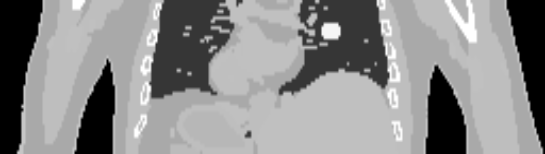
\includegraphics[width=1.0\linewidth]{figures/background_mu_map_example.png}
                    
                    \captionsetup{singlelinecheck=false, justification=raggedright}
                    \caption{Example of a simulated \gls{Mu-Map}, with no motion or noise, of the thorax with a spherical lesion in the lungs. Coronal view.} \label{fig:combined_pet_ct_mu_map_example}
                \end{figure}
                
                \begin{figure}
                    \centering
                    
                    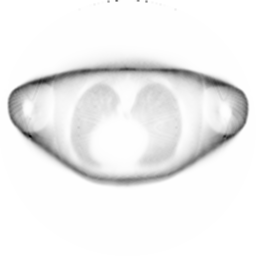
\includegraphics[width=1.0\linewidth]{figures/background_nac_example.png}
                    
                    \captionsetup{singlelinecheck=false, justification=raggedright}
                    \caption{Example of simulated \gls{NAC} \gls{TOF} data, with motion, with no noise randoms or scatters, of the thorax with a spherical lesion in the lungs. Transverse view.} \label{fig:combined_pet_ct_nac_tof_example}
                \end{figure}
                
                \begin{figure} %KT if you're bored (!),I'd put the NAC and AC figures next to eachother
                    \centering
                    
                    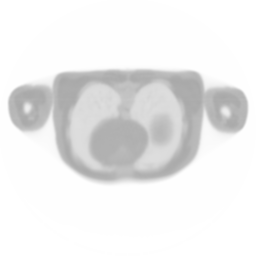
\includegraphics[width=1.0\linewidth]{figures/background_ac_example.png}
                    
                    \captionsetup{singlelinecheck=false, justification=raggedright}
                    \caption{Example of simulated \gls{AC} \gls{NTOF} data, with motion, with no noise, randoms or scatters, of the thorax with a spherical lesion in the lungs. Transverse view.} \label{fig:combined_pet_ct_ac_tof_example}
                \end{figure}
                
                As discussed previously in~\Fref{sec:attenuation} attenuation represents the loss of coincidences by photon interactions in matter. Attenuation is an issue in \gls{PET} as it causes the loss of signal and a degradation in image quality, this is the opposite for \gls{CT} where the modality itself relies on attenuation in order to differentiate anatomical structure, an example of a \gls{Mu-Map} can be seen in~\Fref{fig:combined_pet_ct_mu_map_example}. An example of some \gls{NAC} \gls{TOF} and \gls{AC} \gls{TOF} data can be seen in~\Fref{fig:combined_pet_ct_nac_tof_example} and~\Fref{fig:combined_pet_ct_ac_tof_example} respectively. In order to find reasonable quantitative results the attenuation of the patient must be taken into account in \gls{PET}. %Both \gls{PET} and \gls{CT} follow the Beer-Lambert law. %KT cut last sentence.not  relevant here %ACW done
                
                Methods to acquire \gls{Mu-Map}, for \gls{AC} include; to take a transmission scan of a known point source rotated around the body of the patient prior to the injection of the radiotracer. This allows for the estimation of the attenuation for each angle~\parencite{TransmissionatnBib}. Another method involves the use of the known attenuation from the \gls{CT} scan.
                
                In order to apply the \gls{CT} based \gls{Mu-Map} to \gls{AC} in \gls{PET} first it must undergo either bilinear or trilinear conversion to asses the attenuation coefficient factors, this is because of the relative energy difference of the two modalities~\parencite{Carney2006}. As discussed above in~\Fref{sec:coincidence_processing} and~\Fref{sec:combined_pet_ct} \gls{PET} and \gls{CT} operate at two different energy levels of between between $425$ and $600$ \gls{KeV} and between $40$ and $140$ \gls{KeV} respectively~\parencite{Bettinardi2011}~\parencite{CTattenuationenergyBib}.
                
                Issues with \gls{CT} based \gls{AC} include: Firstly, as mentioned above in~\Fref{sec:combined_pet_ct}, \gls{CT} is acquired sequentially to \gls{PET} rather than simultaneously meaning that there can be mismatches in anatomy between the scans. Secondly, the propagation of any artefacts from the \gls{CT} volume into the \gls{PET} volume. Regardless of these issues \gls{CT} is currently considered to be the gold standard for \gls{Mu-Map} estimation for \gls{AC}. Transmission scans are now very rarely used because of the inclusion of an additional external source, their significant increase in scan time and low image quality compared to \gls{CT}. 
                %KT  Briefly mention MLAA here
                %ACW done
                
                Recently a method to jointly estimate both the activity and attenuation distributions from \gls{PET} data only has been proposed called \gls{MLAA}. This method attempts to reconstruct both distributions by iteratively estimating one distribution while keeping the other one fixed. This can be considered as at each step performing either emission or transmission tomography depending on the distribution being optimised for%. Alternatively, it is also possible to optimise jointly for both distributions in one step
                ~\parencite{Fuin2017}~\parencite{Brusaferri2020JointPET}. A disadvantage of this solution is that without \gls{TOF} information it is a highly ill-posed problem and even with \gls{TOF} data the solution can only be found up to an arbitrary scaling factor. It is also possible for there to be significant cross talk artefacts between the activity and attenuation estimate~\parencite{MLAASalomonBib}~\parencite{MLAADefriseBib}. Additionally, optimising for the attenuation distribution increases the complexity and computational effort required of a reconstruction algorithm.
                
    \longsection{Inverse Problems and Optimisation}{sec:inverse_problems_and_optimisation}
        This section of the thesis introduces the concept of inverse problems. First a definition of an inverse problem is given, including where these may be applicable to the field of \gls{PET}. Next, the definition of an inverse problem is expanded upon by highlighting the difficulty of solving them literally and how this is usually overcome or addressed. The general form of an approach to solving an inverse problem is then given.
            
        The second subsection expands upon the approach given previously to solving inverse problems. Including; defining what an optimisation is, applications of optimisation (for instance, \gls{PET} reconstruction) and listing the requirements of a simple optimisation problem. Next this subsection moves onto addressing the components of an optimisation, including the objective function. The purpose of an objective function in optimisation is presented before a number of common and robust similarity measures are introduced, the merits of different functions is discussed and common applications of specific instances is given. Regularisation is then briefly mentioned before moving onto the optimiser. As with the previous subsection here the purpose of an optimiser is initially introduced before families of optimisation algorithms are compared and variations of these families, as well as their applications, are touched upon. Finally bounds or constraints upon optimisation are mentioned, as well as providing examples of optimisers which can incorporate such functionality.
        
        \subsection{Inverse Problem Concepts} \label{sec:inverse_problem_concepts}
            An inverse problem is one where the original conditions of a system are estimated from its effects. For instance, the data from a \gls{PET} scanner represents the observations of the distribution of the radiotracer, reconstruction is an attempt to find the distribution from these observations.
            
            It is not usually possible to directly invert a problem like this, often due to the complexity or size of a problem (meaning that  the computation time to find an inverse would be large). Thus in these cases the solution can be iteratively optimised for. In order to attempt to find the solution to an inverse problem there are two things which are required; first the forward operator (the forward operator describes the problem in the direction of its initial conditions to its effects) %KT true, but do you understand this? simplify by cutting %ACS I'm pretty sure I do now
            second, ideally, a model of the noise present in the system~\parencite{Brusaferri2020ImprovingInformation}~\parencite{Emond2020ImprovingEffectiveness}. %KT what ``at least''. I'd say ``ideally'' %ACW done
        
        \subsection{Optimisation Concepts} \label{sec:optimisation_concepts}
            Optimisation means to find values that best parametrise a given function based on some criteria or objective. %KT I feel it needs something else ``based on some criteria'' or ``objective'' or ... %ACW done
            For instance, in reconstruction an optimisation could be to find the image that when the forward operator is applied to it the result best matches the measured data. Another example of an optimisation would be to find the motion parameters that when applied to a given image most closely warp that image to match another image. Optimisation is also used in fields such as deep learning to train \glss{NN}, here the optimisation is used to find parameters for a model that maps one set of values to another.%, this will be discussed later in~\Fref{sec:machine_learning_for_pet}.
            
            % CHECK IF PAGE BOUNDARY LOOPS
            \newpage
            
            In order to perform a basic optimisation four components are required; most importantly an objective function (which returns the goodness of the current estimate) and a method to optimise the estimate based on this function are paramount. Additionally, an initial estimate (the closer this is to the ideal estimate then the less computation time is required overall) and a method to determine when optimisation should cease (for instance when the objective function exceeds a threshold or the number of iterations becomes so large) are also necessary. These will be discussed in the following sections in~\Fref{sec:objective_function} and~\Fref{sec:optimiser} respectively.
        
            \subsubsection{Objective Function} \label{sec:objective_function}
                Optimisation of some values requires a function that represents, for instance, the similarity of two measures or the likelihood given a measure. This function is necessary as its output reflects the accuracy of the current estimate. The gradient of the objective function describes the direction in which the optimiser should change the estimate. The optimiser attempts to find a solution by either maximising or minimising the result of applying the objective function and updating the estimate iteratively.
                
                An example of an objective function would be \gls{MAE}. For a vector of some values, \gls{MAE} subtracts the estimated value from the true value, finds the absolute value of this and sums together this value for all values in the vector. The absolute value is taken because the error should be the distance to the true value regardless of if the estimated value is greater or less than the true value. If the estimated values approach the true values then the value of the \gls{MAE} will approach zero. If \gls{MSE} is used then the square of the error is taken rather than the absolute value, taking the square causes the error to increase quadratically as it becomes larger. %KT exponentially? no,quadratically %ACW done
                This can be advantageous as it penalises large errors more than smaller ones, which can lead to a better result in some circumstances. Additionally, the square is differentiable.
                
                More complex objective functions include; \gls{RMSE}, here the square root of \gls{MSE} is taken which scales the value of the error back to the units of the original estimate. Median absolute error is similar to \gls{MAE} however rather than taking the mean of all error values the median is taken instead, this would gave an objective function which is less sensitive to noise or more robust as outliers are diminished or ignored by the median. An objective function which differs more significantly would be \gls{PCC}, here the correlation of the values in the estimate are compared to the measured data, thus if \gls{PCC} was used in an optimisation then it is not guaranteed that the estimate will have the same scale as the measured data but its shape should be similar. \gls{PCC} can be used on very noisy data as it is less sensitive to this noise. \gls{MAE}, \gls{MSE} \gls{RMSE} and \gls{PCC} are usually used in regression-like problems where a line is fit though a data set.
                
                Another example of an objective function would be likelihood. This function for any given sample of data computes the goodness of fit to a statistical model. Strictly speaking, the likelihood is related to the inverse of the goodness of fit. 
                The likelihood function describes a planes whose peak, if there is one distinct peak, %KT???
                represents the combination of model parameter values that maximise the probability of drawing the sample obtained~\parencite{Myung2003TutorialEstimation}. %KT not maximise, it is the probability %ACW done
                \gls{PLL} is often used as the objective function in \gls{PET} reconstruction, this can be seen in~\Fref{sec:pet_image_reconstruction}.
                
                As an additional term to the objective function a regularisation term is often added, summed to the objective function value (after being scaled by an $\epsilon$), in order to decrease sensitivity to noise. An example of a regularisation term is \gls{RDP} used by \gls{GE} in Q.Clear~\parencite{RossQ.Clear}. Another example use be \gls{BE} or \gls{LE} which are used in \gls{IR} to penalise against rapid changes in the \gls{DVF}~\parencite{Modersitzki2009Fair:FlexibleRegistration}.
                
            \subsubsection{Optimiser} \label{sec:optimiser}
                \begin{figure}
                    \centering
                        
                    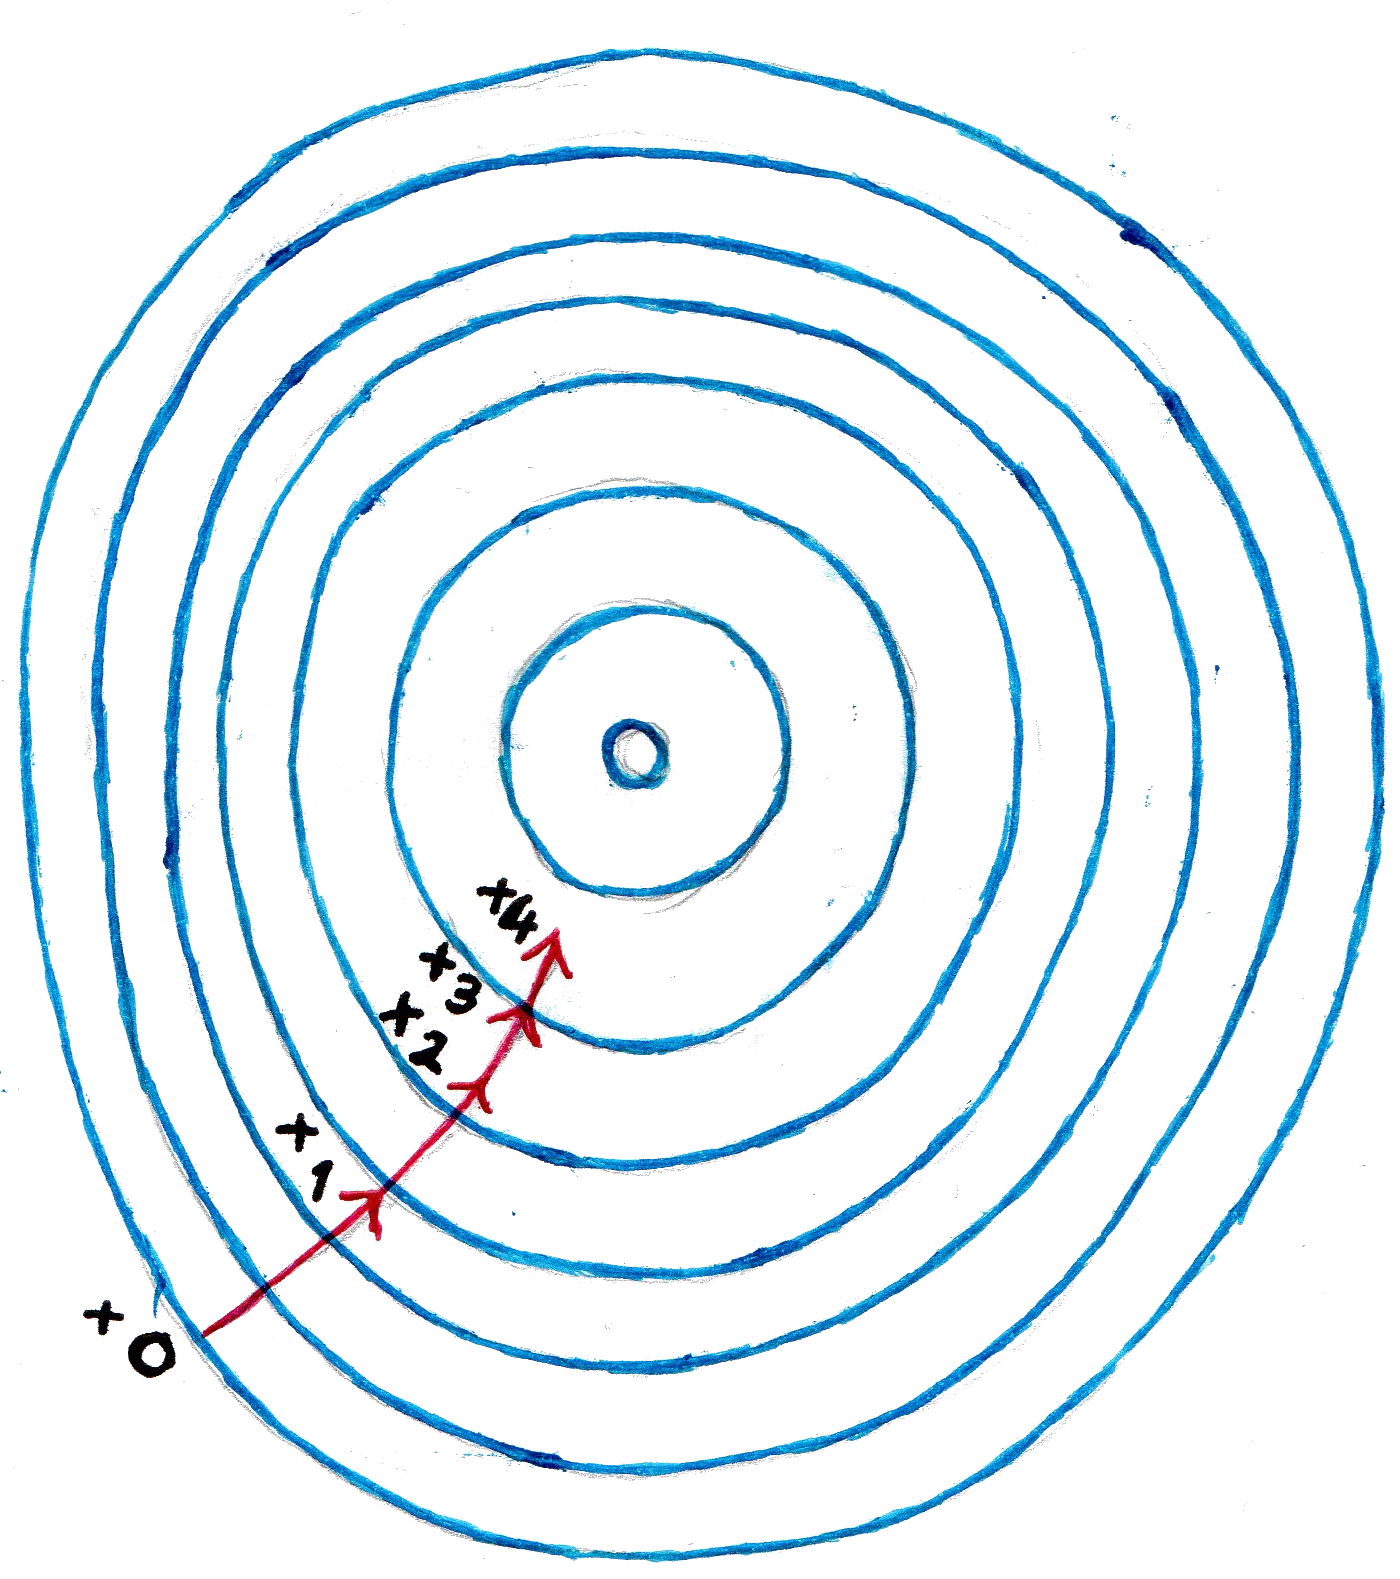
\includegraphics[width=1.0\linewidth]{figures/background_optimisation.png}
                        
                    \captionsetup{singlelinecheck=false, justification=raggedright}
                    \caption{Graphical representation of a \gls{2D} solution space and an optimiser stepping through this space. In the bottom left of this figure the initial estimate for some optimisation can be seen at $x$, the subsequent iterations $1$ through $4$ can then be seen taking this estimate closer to the centre of the contour plot. Here the contour plot could either be showing a maximisation or a minimisation depending on how it is visualised.} \label{fig:optimiser_optimisation}
                \end{figure}
                
                An optimiser takes an estimate of the solution and an objective function, as seen in~\Fref{sec:objective_function} the objective function returns the goodness of the estimate which the optimiser can either maximise or minimise. The direction in which the optimiser updates the estimate is based on the gradient of the objective function. The method by which the optimiser updates the estimate is what differentiates optimisation algorithms.
                
                \gls{GD} is a commonly used family of optimisation algorithms. \gls{GD} itself finds the gradient of the objective function at the current estimate %KT?you mean ``at the current estimate'' %ACW done
                and takes steps, of a given size,  in the direction calculated from the gradient. %which most shrinks the value of the objective function. %KT ``most'' I think is only true for ``Steepest GD''. I'd cut the 2nd half of the sentence %ACW done
                The step size of \gls{GD} can be set to a fixed value or found using a line search which optimises the step size. Momentum can be used as an improvement of \gls{GD} where the current update direction is a linear combination, with a predefined weighting, of the current gradient and the previous update direction.
                
                \gls{SGD} is an extension of \gls{GD} where the current update is calculated using the gradients of a randomly selected subset of the data, %KT of the data (not the estimate) %ACW done
                this is significantly more computationally efficient than \gls{GD} as it reduces the number of calculations needed for each update.
                
                \gls{CG} is another extension of \gls{GD}. Here the direction of subsequent updates are confined so that they are orthogonal to the previous update direction, this can decrease convergence time~\parencite{Tustison2009}. %KT remove the ``can avoid the same issue''. CG also attempts to go to a local minimum %ACW done
                
                \gls{BFGS} and \gls{L-BFGS} are second order optimisers in that they take the second order partial derivatives of the objective function. \gls{BFGS} and its derivatives determine the descent direction by preconditioning the gradient with curvature information. \gls{L-BFGS} is differentiated from \gls{BFGS} in that \gls{BFGS} stores a dense approximation of the inverse Hessian, whereas \gls{L-BFGS} stores a history of a past window of updates. Thus \gls{L-BFGS} uses less memory than \gls{BFGS} and thus can converge faster~\parencite{Fletcher2000PracticalOptimization}.
                
                An optimiser can also be provided with bounds or constraints, a simple bound would be a box bound where the values of the estimate cannot exceed a threshold. \gls{L-BFGS-B} is an implementation of \gls{L-BFGS} which accepts box bounds. This can be useful, for instance, in \gls{PET} reconstruction where it is not expected that negative values should exist, so they could be constrained.
            
    \longsection{PET Image Reconstruction}{sec:pet_image_reconstruction}
        This section of the thesis follows on from the previous section in that it focuses on the inverse problem of \gls{PET} reconstructions specifically. First it shows how \gls{PET} reconstruction is an inverse problem, by likening aspects of the reconstruction problem to those presented previously, before elaborating on the two general families of reconstruction algorithm. Analytical and numerical approaches to \gls{PET} reconstruction are discussed and finally a common output scale from this process is highlighted.
            
        The second subsection expands upon the numerical approach (or optimisation) to \gls{PET} reconstruction given previously. Initially the advantages and disadvantages of iterative \gls{PET} reconstruction in general are introduced. Then common algorithms are described and their operation, advantages and disadvantages are compared. 
        
        \subsection{Introduction} \label{sec:pet_image_reconstruction_introduction}
            \gls{PET} image reconstruction is an inverse problem, as stated in~\Fref{sec:inverse_problem_concepts}. This means that a \gls{PET} reconstruction algorithm takes as an argument the effects of the \gls{PET} acquisition system and attempts to determine its initial conditions, for instance the distribution of the radiotracer.
            
            There are two main families of methods through which a \gls{PET} reconstruction can be performed. First there are analytical \gls{PET} reconstruction algorithms, an analytical solution frames the problem in a better understood form and attempts to calculate the exact solution.% As stated in~\Fref{sec:analytic_image_reconstruction}.
            Secondly there are numerical solutions, for instance, iterative \gls{PET} reconstruction. Generally a numerical solution takes guesses at the solution and tests if the problem is solved. Numerical approaches to solving inverse problems in general are discussed in~\Fref{sec:inverse_problem_concepts} and iterative \gls{PET} reconstruction algorithms are discussed in~\Fref{sec:iterative_image_reconstruction}.
            
            The data output from a \gls{PET} scan are usually expressed in \gls{KBq/mL}, however for pseudo quantitative analysis the values are usually normalised to \gls{SUV} by dividing the activity by, for instance, the mass of the patient and the injected activity. %KT previous sentence belongs in image recon section, not where you discuss the measured data %ACW done
        
%        \subsection{Analytic Image Reconstruction} \label{sec:analytic_image_reconstruction}
            % mention briefely FBP ?
            %KT no! cut. I didn't read it
            %ACW done
%            \begin{figure}
%                \centering
                    
%                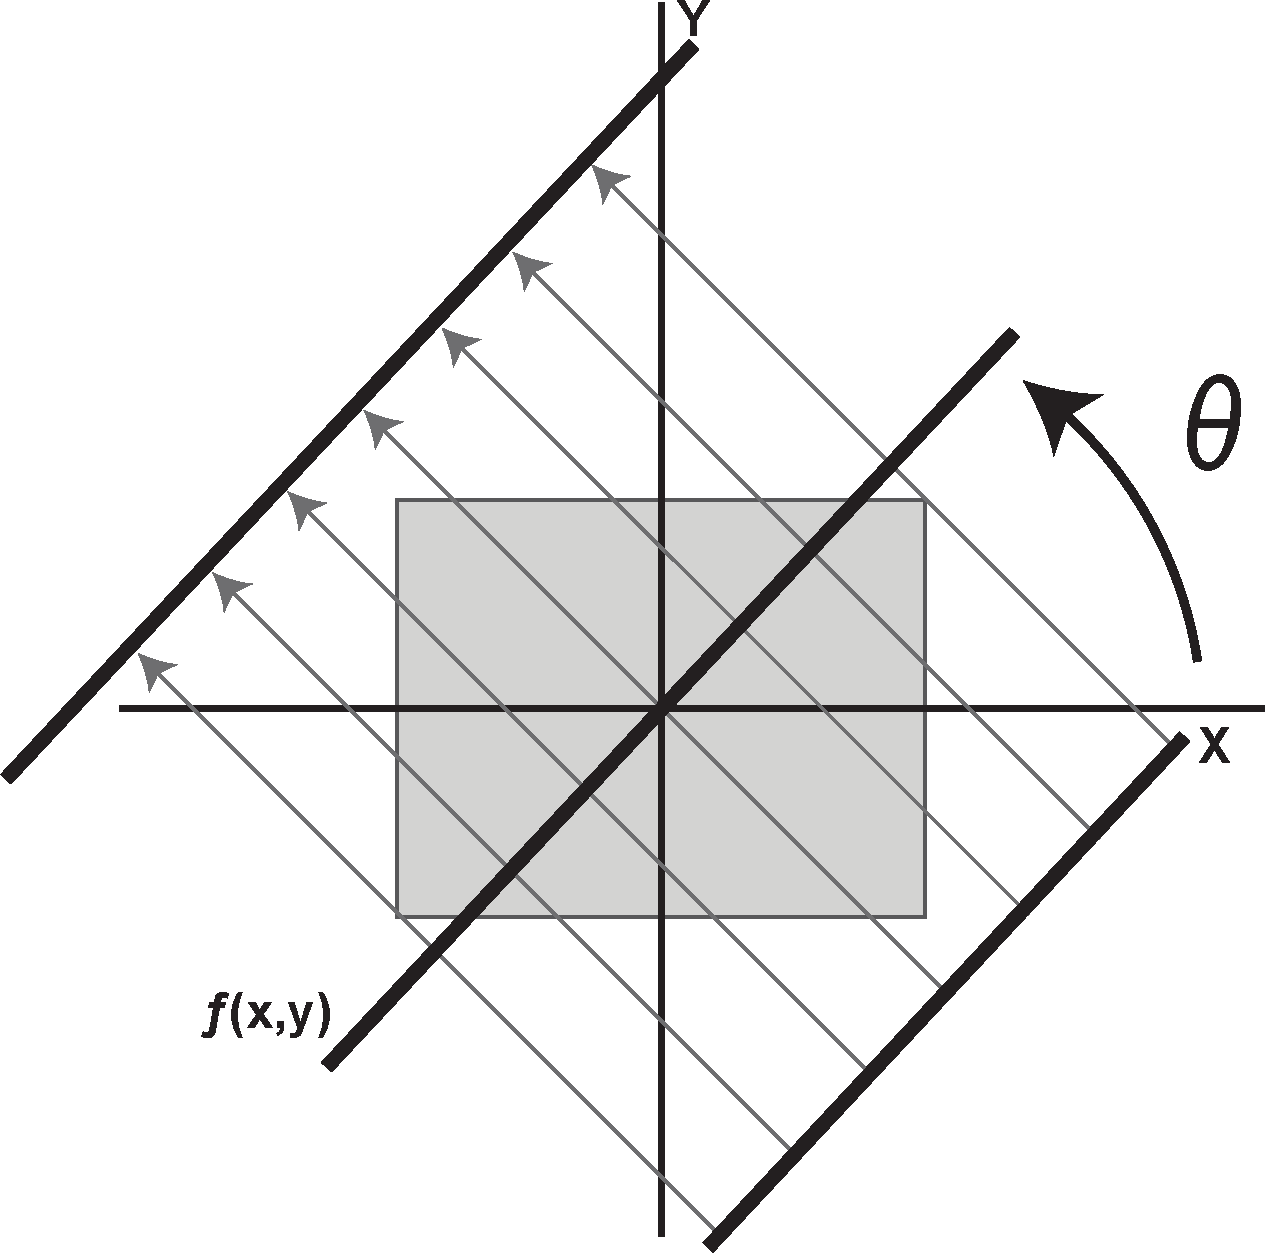
\includegraphics[width=1.0\linewidth]{figures/background_radon_transform.png}
                    
%                \captionsetup{singlelinecheck=false, justification=raggedright}
%                \caption{Graphical representation of the Radon transform for one angle $\theta$. The Radon transform computes projections of some data along specified directions. Here, this figure shows the computation of a set of line integrals for the function $f(x, y)$, usually from multiple sources of parallel beams. To form a full image the Radon transform rotates the source around the centre of the image. This figure specifically shows projections for a simple \gls{2D} image along horizontal and vertical components $x$ and $y$.} \label{fig:analytic_image_reconstruction_radon_transform}
%            \end{figure}
            
%            \begin{figure}
%                \centering
                
%                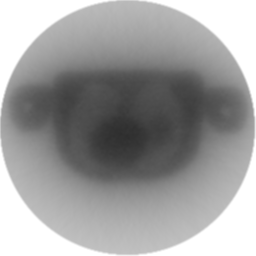
\includegraphics[width=1.0\linewidth]{figures/background_bp_example.png}
                
%                \captionsetup{singlelinecheck=false, justification=raggedright}
%                \caption{Example of a simulated \glss{AC} \gls{NTOF} \gls{BP} reconstruction, with motion and noise, with no randoms or scatters, of the thorax with a spherical lesion in the lungs. Transverse view.}
%                \label{fig:analytic_image_reconstruction_bp_example}
%            \end{figure}
            
%            \begin{figure}
%                \centering
                
%                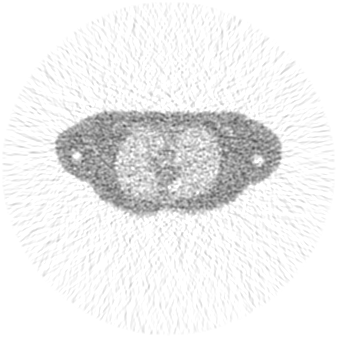
\includegraphics[width=1.0\linewidth]{figures/background_fbp_example.png}
                
%                \captionsetup{singlelinecheck=false, justification=raggedright}
%                \caption{Example of a simulated \glss{AC} \gls{NTOF} \gls{FBP} reconstruction, with motion and noise, with no randoms or scatters, of the thorax with a spherical lesion in the lungs. Transverse view.}
%                \label{fig:analytic_image_reconstruction_fbp_example}
%            \end{figure}
            
%            An analytic solution is one which offers a direct mathematical method through which one thing can be transformed to another. All analytical solutions can have a proof. An analytical solution for \gls{PET} reconstruction is \gls{BP}, in \gls{2D} \gls{BP} is the inverse Radon transform. This can be seen in~\Fref{fig:analytic_image_reconstruction_radon_transform}. To apply the inverse Radon transform to a \gls{2D} sinogram; first the rows of the sinogram, corresponding to $\SI{0}{^{\circ}}$ through $\SI{180}{^{\circ}}$, are taken individually and have the Fourier transform applied to them. Then the result of this is reshaped to polar coordinates so that each row is the diameter of a circle and a \gls{2D} Fourier transform is applied giving the final output image. The Fourier transform decomposes a function into its constituent frequencies. The \gls{2D} Fourier transform of a function computed along a line is equivalent to the 1D Fourier transform of the Radon transform along that line. This is called projection slice theorem. 
            
%            \gls{FBP} was proposed as a solution to some of the issues apparent in \gls{BP}, like the fact that \gls{BP} suffers from low frequency blurring. In \gls{FBP} a high pass ramp filter is applied to the sinogram before it is Fourier transformed, thus removing some low frequency information or blurring. A low pass ramp filter can also be applied at the same time which removes some high frequency information or noise, this then would be a band pass filter. An example of a \gls{BP} and \gls{FBP} reconstruction can be seen in~\Fref{fig:analytic_image_reconstruction_bp_example} and~\Fref{fig:analytic_image_reconstruction_fbp_example}. Because of its speed and good quantitative results \gls{FBP} was the gold standard of \gls{PET} \gls{IR}, however because of the issues mentions above it has now almost entirely been replaced by iterative reconstruction methods. \gls{FBP} is now almost solely used in longitudinal studies which started before the use of iterative reconstruction methods became prevalent~\parencite{FBPReviewBib}~\parencite{PETCTReviewBib}.
            
%            \gls{BP} and \gls{FBP} reconstruct a low quality image but are computationally fast. \gls{BP} will usually result in there being numerous streak like artefacts in the output image, the artefacts are exacerbated as noise increases. Artefacts can be caused because neither \gls{BP} nor \gls{FBP} account for the stochastic nature of the acquisition process, neither do they account for other factors such as positron range as discussed in~\Fref{sec:attenuation}.
            
            
        \subsection{Iterative Image Reconstruction} \label{sec:iterative_image_reconstruction}
            \begin{figure}
                \centering
                
                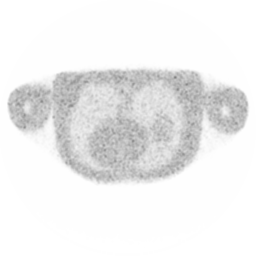
\includegraphics[width=1.0\linewidth]{figures/background_osem_example.png}
                
                \captionsetup{singlelinecheck=false, justification=raggedright}
                \caption{Example of a simulated \gls{AC} \gls{NTOF} \gls{OSEM} reconstruction, with motion and noise, with no randoms or scatters, of the thorax with a spherical lesion in the lungs. Transverse view.}
                \label{fig:iterative_image_reconstruction_osem_example}
            \end{figure}
            
            %As discussed above in~\Fref{sec:inverse_problems_and_optimisation} an inverse problem, which \gls{PET} reconstruction is, can be solved by an iterative optimisation problem. In order to implement an iterative optimisation problem a few criteria must first be met; a forward operator which takes an image and return the projections which would result from acquiring the image is required. As discussed above in~\Fref{sec:optimisation_concepts} an objective function to assess the accuracy of the fit and an optimisation algorithm to improve the fit are required. Also, an initial estimate, which could be a volume the size of the output image filled with ones or zeros, and some method to cease execution, for instance stopping when the objective function reaches a certain value or the number of iterations exceeds a threshold, are also necessary. %KT cut all this here as strong overlap with previous section. Move statement about initial estimate and stopping criteria there. %ACW done

            %KT cut some stuff if cutting analytic recons above
            An iterative method has the advantage that the model which is used can take into account the noise properties of the data and also the physical properties of the scanner. The noise associated with \gls{PET} is often assumed to be Poisson distributed. However, iterative methods have the disadvantage that they require substantial computational effort to execute when compared to analytical reconstruction.
            
            %\gls{ML} is a commonly used objective function for iterative \gls{PET} reconstruction. This builds on the concepts, specifically \gls{MLE}, mentioned in~\Fref{sec:objective_function}. %KT cut previous sentence. no need to repeat all the time %ACW done
            \gls{ML} is often combined with the \gls{EM} algorithm for the optimisation of the model parameters and in this case is called \gls{MLEM}~\parencite{MLEMBib}~\parencite{PETMLEMBib}~\parencite{PETMLEM2Bib}. When maximising the likelihood the natural logarithm of the likelihood, also known as the log-likelihood, is taken for computational efficiency. The output from \gls{MLEM} commonly has a Gaussian blur applied in order to smooth noise~\parencite{PETMLEMFiltBib}. Disadvantages associated with \gls{MLEM} include, for noisy data iterating for too long can cause the output to accentuate the noise present in the data, one way to avoid this is to purposefully cease iterating early before the noise can take over the image~\parencite{PETMLEMTerminationBib}. Another issue is that \gls{MLEM} is exceptionally slow even when compared to other iterative algorithms. %KT ``as mentioned earlier, as will be discussed below''. only the latter I guess %ACW done
            
            To combat the slow execution speed of \gls{MLEM} \gls{OSEM} was developed. In \gls{OSEM} the \gls{LOR} or detector pairs of the scanner are binned into a number of subsets. This is in contrast to \gls{MLEM} where there is logically one subset, \gls{MLEM} would be applied to all \gls{LOR} or detector pairs simultaneously. However, in \gls{OSEM} the \gls{LOR} or detector pairs could be binned into at least two subsets. \gls{MLEM} is then applied to each subset, in a specific order, sequentially~\parencite{Hudson1994}. Because the image is updated after each iteration of \gls{MLEM} on each subset of \gls{OSEM} then the execution speed of \gls{OSEM} is increased by the number of subsets used. However, if% more than two 
            subsets are used %KT even with 2 actually... %ACW done
            then  \gls{OSEM} will converge to a limit cycle around true convergence~\parencite{Mettivier2011}. If a reasonable number of subsets are used it has been found that \gls{OSEM} will accelerate \gls{MLEM} without affecting the accuracy of quantification too drastically~\parencite{Morey2013}. An example of an \gls{OSEM} reconstructed image can be seen in~\Fref{fig:iterative_image_reconstruction_osem_example}.
            
    \longsection{Respiratory Motion in PET}{sec:respiratory_motion_in_pet}
        % general intro
        This section of the thesis introduces the problem of \gls{RM} in \gls{PET}/\gls{CT}. First it addresses how \gls{RM} presents specifically in reconstructed \gls{PET} volumes and what this can mean for clinical diagnosis. Next the issue of \gls{RM} in combined \gls{PET}/\gls{CT} is highlighted and the challenges associated with the misalignment of the data between modalities is touched on, including how this could negatively impact the \gls{AC} reconstructed \gls{PET} volume (issues introduced by the \gls{PET}/\gls{CT} workflow in the clinic are also presented).
            
        The second subsection expands upon the challenges introduced by \gls{RM} in the combined \gls{PET}/\gls{CT} workflow and lists some methods from the clinic and the literature which have been developed to combat this.
        
        \subsection{Respiratory Motion Artefacts} \label{sec:respiratory_motion_artefacts}
            % have a look at https://www.sciencedirect.com/science/article/pii/S0001299808000214?via%3Dihub
            
            \begin{figure}
                \centering
                
                
\includegraphics[width=1.0\linewidth]{figures/background_motion_artefact_example.png}
                
                \captionsetup{singlelinecheck=false, justification=raggedright}
                \caption{Example of a simulated \gls{AC} \gls{NTOF} \gls{OSEM} reconstruction, with motion, with no noise, randoms or scatters, of the thorax with a spherical lesion in the lungs. Coronal view.}
                \label{fig:respiratory_motion_artefacts_motion_artefact}
            \end{figure}
            
            \begin{figure}
                \centering
                
                
\includegraphics[width=1.0\linewidth]{figures/background_single_mu-map_ac_example.png}
                
                \captionsetup{singlelinecheck=false, justification=raggedright}
                \caption{Example of a simulated single \gls{Mu-Map} \gls{AC} \gls{NTOF} \gls{OSEM} reconstruction, with motion, with no noise, randoms or scatters, of the thorax with a spherical lesion in the lungs. Coronal view.}
                \label{fig:respiratory_motion_artefacts_single_mu-map_ac}
            \end{figure}
            
            A static single bed position acquisition on a conventional \gls{PET} scanner takes, on average, approximately \SI{120}{\second}. This means that, because the patient is in \gls{RM} throughout the acquisition, then the result of the scan will contain data from different respiratory states. During the different respiratory states the position and volume of the lungs, diaphragm and any lesion will change. If the data is reconstructed without accounting for this then there will be the presence of blurring artefacts (especially prevalent around the anatomy that is moving the most, such as the diaphragm). %This would be expected as the data, in this case, represents as if the respiratory states had been summed together. %KT let's cut the previous sentence in an attempt to be less verbose :-) %ACW done
            An example of a \gls{PET} reconstruction with motion artefacts can be seen in~\Fref{fig:respiratory_motion_artefacts_motion_artefact}, notice the blurring above the diaphragm on the right side of the figure. Artefacts originating from the moving anatomy pose the largest challenge in imaging of the thorax~\parencite{LungMotionArtefactBib}~\parencite{PETCTArtifactBib}.
            
            The artefacts caused by \gls{RM} lead to issues clinically with cancer staging and follow up. This is because the size of the tumour is often overestimated and the activity underestimated (the activity in the lesion is spread over more voxels) thus it has the capacity to cause lesions to potentially be missed due to reduced detectability~\parencite{LungMotionJudgmentErrorsBib}. %KT and lesions potentially to be missed (i.e reduced detectability) %ACW done
            
            If \gls{AC} is used then the position of the \gls{Mu-Map} in relation to the \gls{PET} data also poses an issue. Where the \gls{Mu-Map} does not match the position of the anatomy then it will cause either under or over-correction of the attenuation. This can cause a type of artefact often referred to as a banana artefact due to the shape of the shadow that it causes to appear above the diaphragm~\parencite{LungMotionDiaphragmBaiBib}. An example of this can be seen in~\Fref{fig:respiratory_motion_artefacts_single_mu-map_ac}. Notice the black arc shaped artefact over the diaphragm and on the heart. The mismatch of the \gls{Mu-Map} and \gls{PET} data does not just cause this artefact but it can also change the expectation and thus the quantification of the reconstructed image. To combat intra-\gls{Mu-Map} motion the patient will often be asked to hold their breath, if they can, as the \gls{CT} acquisition can last for only between \SI{2.0}{\second} and \SI{3.0}{\second}~\parencite{Nyflot2015}. An issue with this is, that often the breath hold \gls{CT} will be taken at full inspiration, if this \gls{Mu-Map} is then used to correct for attenuation in data that is in a respiratory phase other than full inspiration then a lot of this anatomy will have been moved into the \gls{FOV} (it is not present in the \gls{Mu-Map}). Furthermore, when a patient is asked to hold their breath they often inhale deeper than they otherwise would, meaning that this \gls{Mu-Map} can be in an unrealistic respiratory state that will not be represented in the \gls{PET} data taken during free breathing. %KT this last sentence is incorrect. ``intra-mu-map'' motion can indeed by circumvented lrgely by breathold (as it's a CT). however, most people would do this at full inspiration, and then you get into serious trouble. %ACW done
            
        \subsection{Respiratory Motion Challenges in Combined PET/CT Imaging} \label{sec:respiratory_motion_challenges_in_combined_pet_ct_imaging}
            To overcome the issues mentioned in~\Fref{sec:respiratory_motion_artefacts}, specifically related to the mismatch between \gls{Mu-Map} and \gls{PET} data a number of solutions have been proposed:
            
            \begin{itemize}
                \item Firstly, a method which acquires \gls{PET} data over a prolonged acquisition and throws away any data where the patient is in a position other than the one that corresponds most closely to the breath hold \gls{CT} \gls{Mu-Map}. For this all data which is not at full inspiration would be removed~\parencite{Liu2010}~\parencite{Grootjans2014}. %KT I'd rather say that the CT is then at breathhold first. %ACW done
                The breath hold \gls{CT} \gls{Mu-Map} could then be warped to this data~\parencite{LungMotionBreathHoldBib}. An advantage of this approach is that it would not only correct for the misalignment of \gls{Mu-Map} and \gls{PET} data but it could also eradicate most blurring associated with averaging over respiratory phases. A disadvantage is that, either there would be substantially more noise in the reconstructed data (if the acquisition was the same length as a standard one) or the acquisition could take significantly longer (to acquire an equivalent number of counts), as so much data is being removed~\parencite{Nehmeh2008a}. Additionally, dynamic scans would not be possible with this correction method. This is because the radiotracer kinetics could be shorter than one respiratory cycle and thus would be lost when those parts of the acquisition are removed.
                
                \item Secondly, a variation of the previous method has been proposed, where the \gls{PET} data is separated into individual images representing the separate respiratory phases and warped to a common respiratory phase (seen in~\Fref{sec:image_registration}). The breath hold \gls{CT} \gls{Mu-Map} could then be warped to the same common respiratory phase. This method provides the advantage over the first in that it uses all of the data from the \gls{PET} acquisition and provides a more robust reconstruction~\parencite{4DPhaseMatchedReconBib}. A disadvantage is, that the reconstruction of each respiratory phase is likely to contain more noise than if all of the \gls{PET} data was reconstructed simultaneously. This is because the iterative reconstruction algorithm (seen in~\Fref{sec:iterative_image_reconstruction}) is non-linear (analytical reconstructions are linear but are not used clinical anymore) and summing reconstructed volumes is not equivalent to summing projection data, reconstructing and then summing again. %KT true, but you then first need to say that the images are summed again. %ACW done
                In addition, the higher levels of noise in the reconstructed data can pose a problem when attempting to warp the \gls{Mu-Map} to them.
                
                \item Finally, a method where the reconstruction and motion parameters can be estimated simultaneously, directly from the \gls{PET} data, for one breath hold \gls{CT} \gls{Mu-Map} has been recently proposed~\parencite{JacobsonFesslerMotionCorrectionBib}~\parencite{MLAARezaeiBib}~\parencite{Bousse2016a}. Here, the \gls{PET} data is split into the respiratory phases, as above. Then the method iterates between a reconstruction step (seen in~\Fref{sec:iterative_image_reconstruction}) and a motion parameter estimation step (seen in~\Fref{sec:image_registration}) where the same parameters are used to warp both the \gls{PET} data and the \gls{Mu-Map} for each respiratory position. Thus the \gls{Mu-Map} does not have to correspond to any one respiratory phase as each set of \gls{PET} data will be reconstructed at the position of the \gls{Mu-Map}. This method works especially well when \gls{TOF} data is available~\parencite{Bousse2016}. A disadvantage of this method is that it takes more computation than the above methods and that it has not been as extensively evaluated.
            \end{itemize}
    
    \longsection{Motion Correction for PET}{sec:motion_correction_for_pet}
        This section of the thesis concerns all things \gls{MC} (specifically when applied to \gls{PET}). The first subsection introduces the concept of \gls{IR}, initially highlighting its similarity to \gls{PET} reconstruction (in the sense that they are both optimisation problems) before moving on to discussing the classification of motion types and how they can be corrected. The first kinds of deformation, briefly mentioned, are \gls{RD} and \gls{AD} then \glss{NRD} are introduced and classic approaches to alleviating them are highlighted, including parametric and nonparametric registration and methods of regularising them are touched on.
        
        The second subsection moves on to introduce the concept of respiratory gating, including both amplitude and phase gating before the third subsection which explains how the \glss{SS}, which are used in respiratory gating, are acquired. Firstly methods incorporating external devices to extract \glss{SS} are highlighted, including using the \gls{RPM}, then moving onto \gls{DD} methods. \gls{PCA} is explained as a dimensionality reduction technique and its use for acquiring \glss{SS} directly from \gls{PET} acquisition data is provided.
        
        The fourth subsection gives examples of how to combined \gls{IR} and respiratory gating, specifically mentioning pair-wise and group-wise registration before an extension of vanilla \gls{IR} is introduced in the fifth subsection. Here \gls{MM}, both iteratively and simultaneously with \gls{IR} is introduced including simple \gls{MM} (for instance, a linear regression of \glss{DVF} and \gls{SS}) as well as more complex \gls{MM} approaches. Furthermore, different types of \gls{RCM} and their formation, advantages and disadvantages are touched on.
        
        The final subsection is related to the actual application of \gls{MC}, for instance, how and where it is applied. This includes highlighting the benefits of both a post reconstruction and iterative with reconstruction schema.
    
        \subsection{Image Registration} \label{sec:image_registration}
            \gls{IR} is an optimisation problem which attempts to warp one image (called the dynamic image) to another image (called the static image). The way that one image is warped to another image is through the use of a transformation (or \gls{DVF}). There are  different kinds of deformations including \glss{RD} and \glss{NRD} which will be discussed in the following sections in~\Fref{sec:rigid_deformation} and~\Fref{sec:non_rigid_deformation} respectively. These deformations directly deform or warp the dynamic image so that it best matches the static image. %If there are multiple dynamic images then the optimisation will produce a transformation for each image.
            The images used for \gls{IR} do not necessarily need to be from the same modality and as such \gls{CT} data can be registered to \gls{PET} data or vice versa. A common use for \gls{IR} in medical imaging is to aid in the process of \gls{MC}.
            
            As discussed in~\Fref{sec:optimisation_concepts} an optimisation requires an objective function. In the case of \gls{IR} the most common objective functions are \gls{MSE}, \gls{CC} and \gls{MI}. \gls{MSE} is discussed in~\Fref{sec:objective_function} but simply assumes that once the dynamic image has been deformed to the static then the images should be identical, thus \gls{MSE} is best used when the only difference between the two images is from, for instance, motion and not from a change in modality. \gls{CC} and \gls{MI} are less reliant on the specific intensity values of an image and instead look for relationships between intensities, thus they are more suitable to registering between different modalities than \gls{MSE}~\parencite{Hill2001}~\parencite{Oliveira2014}.
            
            One difference between the optimisation for \gls{PET} reconstruction and for \gls{IR} is that the stochastic nature of the data is not usually taken into account in the model for \gls{IR}.
            
            \subsubsection{Rigid Deformation} \label{sec:rigid_deformation}
                \begin{figure}
                    \centering
                    
                    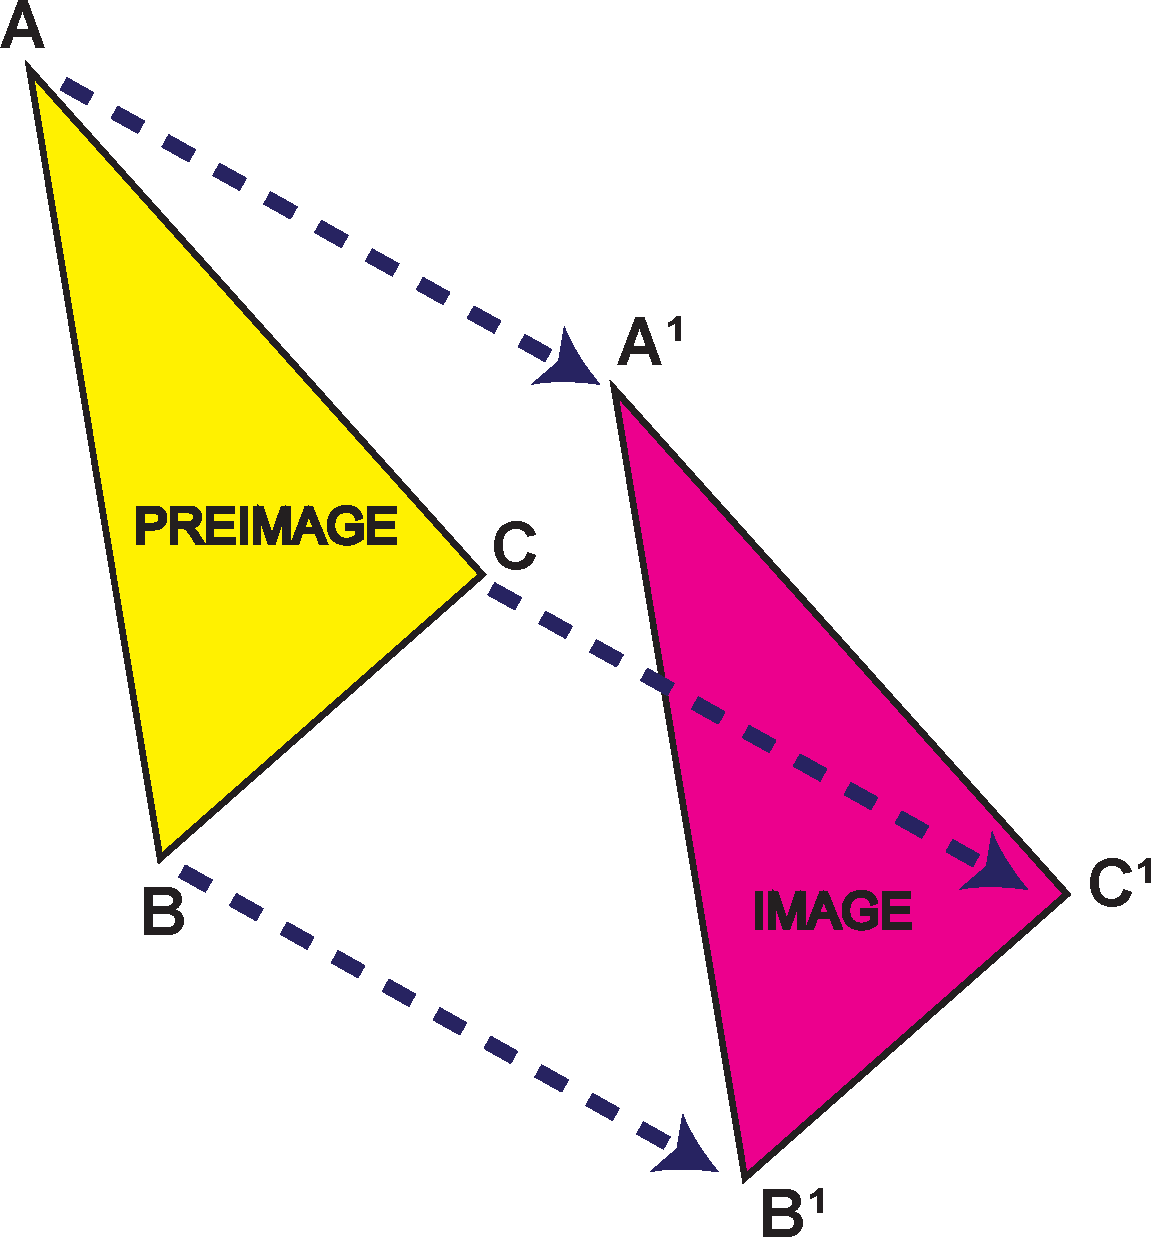
\includegraphics[width=1.0\linewidth]{figures/background_rd.png}
                    
                    \captionsetup{singlelinecheck=false, justification=raggedright}
                    \caption{Graphical representation of a \gls{RD}. On the left a triangle with vertices $A$, $B$ and $C$ can be seen, this triangle undergoes a \gls{RD} (a translation down and to the right) to a triangle, on the right, with vertices $A'$, $B'$ and $C'$.} \label{fig:rigid_transformations_rd}
                \end{figure}
                
                \begin{figure}
                    \centering
                    
                    \includegraphics[width=0.9\linewidth]{figures/background_ad.png}
                    
                    \captionsetup{singlelinecheck=false, justification=raggedright}
                    \caption{Graphical representation of an \gls{AD}. In the centre a cyan leaf can be seen which undergoes an \gls{AD} (a translation down and to the left, a rotation anticlockwise and a scale down) to a red leaf, on the left. The cyan leaf also undergoes an \gls{AD} (a translation down and to the right, a rotation clockwise, a scale down and a skew) to a blue lead, on the right.} \label{fig:rigid_transformations_ad}
                \end{figure}
                
                A \gls{RD} could be a rotation or a translation of the entire contents of an image where the same rotation or translation is applied at every point. A \gls{RD} is one where the euclidean distance between every pair of points in the image is consistent before and after the deformation is applied, this can be seen in~\Fref{fig:rigid_transformations_rd}. \glss{RD} are a subset of a type of deformation called an \gls{AD}. A \gls{3D} \gls{RD} has six degrees of freedom, being rotation and translation in every axis, whereas a \gls{3D} \gls{AD} has $12$ degrees of freedom, rotation, translation, scaling and sheering in every axis. An \gls{AD} does not guarantee that the euclidean distance between pairs of points are maintained, this can be seen in~\Fref{fig:rigid_transformations_ad}.
                
                \glss{RD} are often used in medical imaging where the anatomy which is being registered is not expected to undergo individual internal motion, for instance \glss{RD} are often used in the registration of patient head motion~\parencite{Hill2001}. \glss{AD} are not often used in medical imaging as anatomy does not usually deform in ways that \glss{AD} can capture but \glss{RD} cannot, although an \gls{AD} can be used as an initial estimate for fitting a more complex \gls{NRD}.
                
                The output from a \gls{RD} or \gls{AD} is usually the values from the six or $12$ value transformation matrix, respectively, and as such they do not take up much computational memory or storage.
                
            \subsubsection{Non-Rigid Deformation} \label{sec:non_rigid_deformation}
                \begin{figure}
                    \centering
                    
                    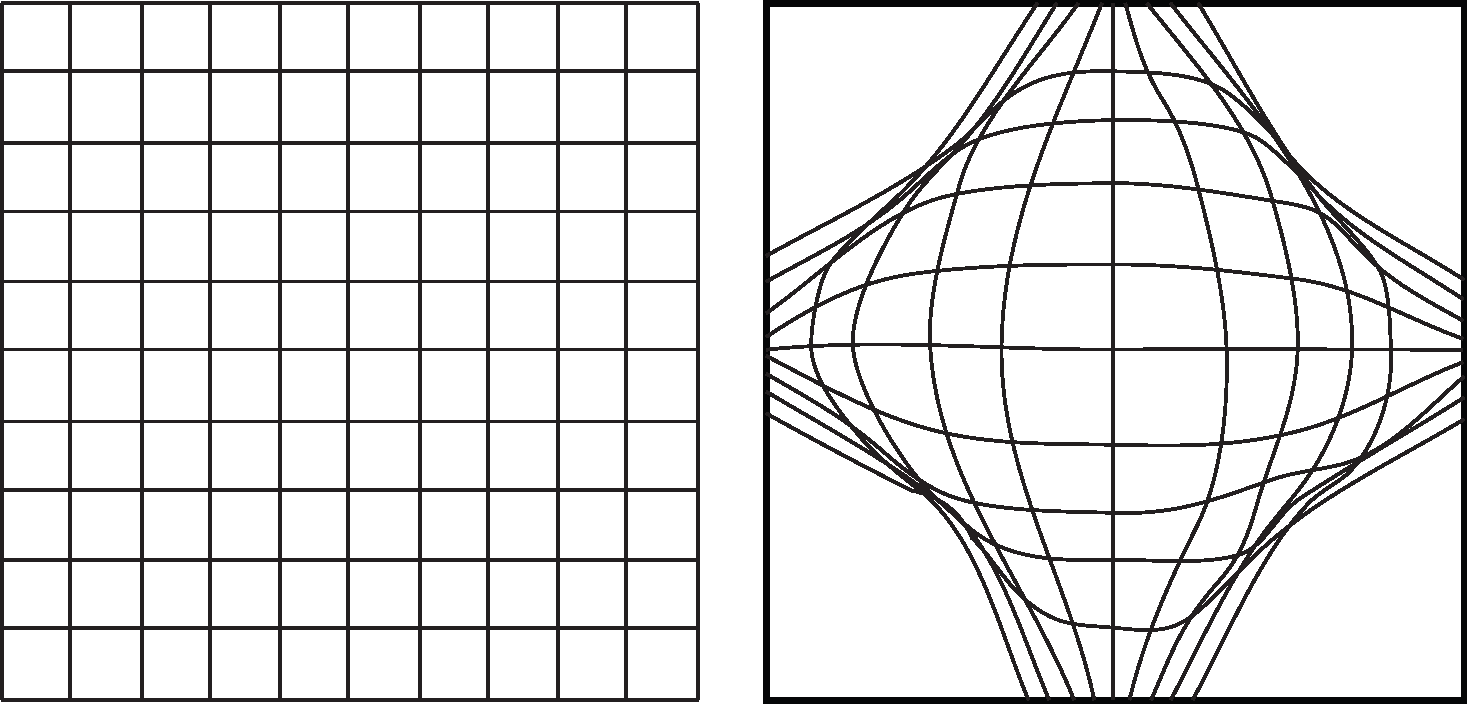
\includegraphics[width=1.0\linewidth]{figures/background_nrd.png}
                    
                    \captionsetup{singlelinecheck=false, justification=raggedright}
                    \caption{Graphical representation of a \gls{NRD}. On the left a grid can be seen, this grid undergoes a \gls{NRD} to the grid on the right.} \label{fig:non_rigid_deformation_nrd}
                \end{figure}
                
                A \gls{NRD} is one where the euclidean distance between pairs of points is not maintained, this can be seen in~\Fref{fig:non_rigid_deformation_nrd}. Notice that the euclidean distance between where the lines of the grids intersects changes between the grid on the left and the grid on the right. %For example the motion of a fluid is a \gls{NRD} as pairs of points can move past each other by different amounts.
                \glss{NRD} are commonly seen in medical imaging in \gls{RM} as the diaphragm and lungs experience sliding motion and displace different parts of the patient's anatomy by different amounts over the respiratory cycle. A \gls{NRD} is often represented by a \gls{DVF} which is, in the simplest case, a volume (the same size, with the same number of elements, as the data) where each 'voxel' contains a vector that points either from the voxel in the dynamic image to the same voxel (anatomically, not literally) in the static image or vice versa.
                
                However, for reasons of computational efficiency (and usually to regularise the \gls{IR} optimisation, somewhat) the \gls{DVF} can be parameterised. One parameterisation could be to use \glss{CP} on a \gls{CPG} which are interpolated using, for instance, linear or B-spline interpolation to find the vector to be applied at each voxel~\parencite{Bardinet1996}~\parencite{Rueckertetal.1999}~\parencite{Mattes2003}~\parencite{JacobsonFesslerMotionCorrectionBib}. There are also \gls{IR} methods which forego parameterisation and instead directly fit the \gls{DVF}, for instance Daemon registration (also known as nonparametric registration algorithms)~\parencite{Vercauteren2009DiffeomorphicRegistration.}.
                
                Regularisation terms are often employed for \glss{NRD} \gls{IR} as otherwise with a high resolution \gls{CPG} it is possible for the optimisation to fit the noise present in the data rather than fitting the motion, as discussed in~\Fref{sec:optimisation_concepts}. One common form of regularisation is a smoothness penalty, for instance \gls{TPS}, \gls{BE} or \gls{LE}. Here, simply, the term is calculated as the integral of the square of the second derivative of the \gls{DVF}. This term is multiplied by some value $\epsilon$ representing the weighting of this penalty term and then the scaled term is summed to the current value of the objective function. This regularisation term attempts to enforce that adjacent \glss{CP} should not rapidly change, with regards to one another, as this type of motion is unlikely physically~\parencite{Duchon1977SplinesSpaces}. In the case of nonparametric registration, a Gaussian smoothing of the input data is sometimes used for regularisation~\parencite{Vercauteren2009DiffeomorphicRegistration.}.
        
        \subsection{Respiratory Gating} \label{sec:respiratory_gating}
            % brief intro
            
            \begin{figure}
                \centering
                    
                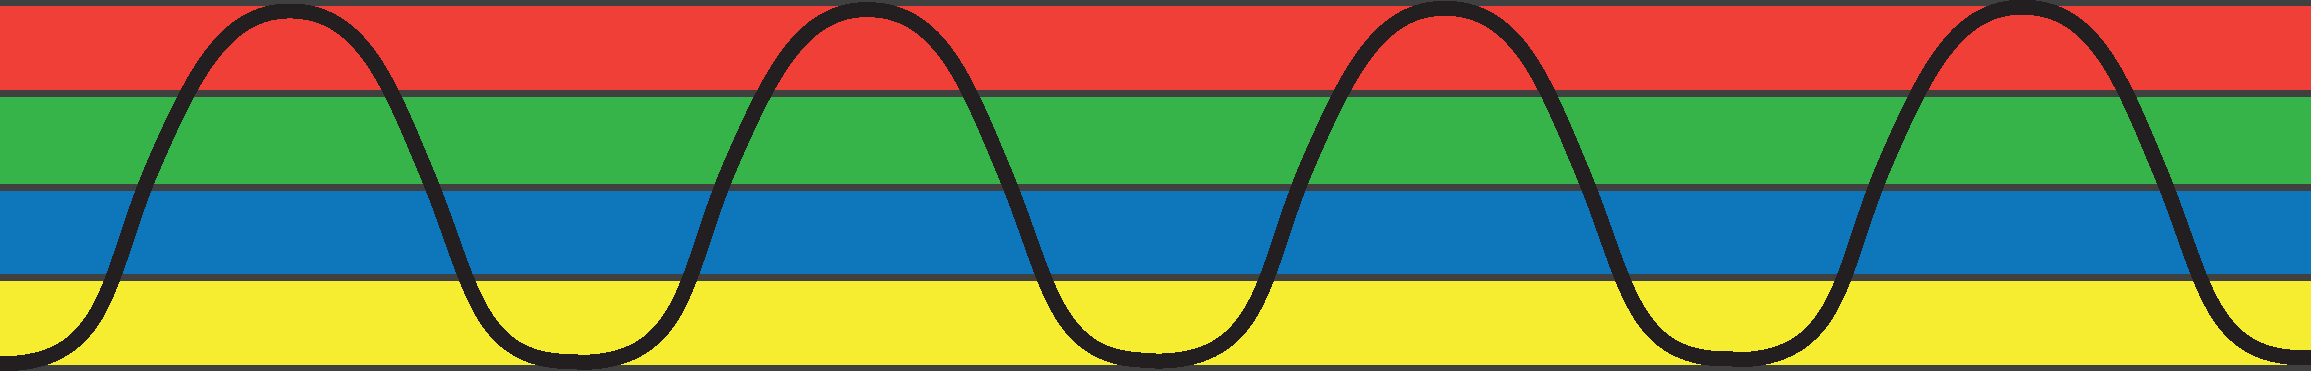
\includegraphics[width=1.0\linewidth]{figures/background_amplitude_gating.png}
                    
                \captionsetup{singlelinecheck=false, justification=raggedright}
                \caption{Graphical representation of amplitude gating. Here the red pseudo sinusoidal signal represents the \gls{SS} and the horizontal lines, colour coded differently, represent the amplitude gates that the data upon the \gls{SS} would be binned into.} \label{fig:respiratory_gating_ampliude_gating}
            \end{figure}
            
            \begin{figure}
                \centering
                    
                \includegraphics[width=1.0\linewidth]{figures/background_full_phase_gating.png}
                    
                \captionsetup{singlelinecheck=false, justification=raggedright}
                \caption{Graphical representation of phase gating. Here the red pseudo sinusoidal signal represents the \gls{SS} and the vertical lines, colour coded differently, represent the phase gates that the data upon the \gls{SS} would be binned into.} \label{fig:respiratory_gating_full_phase_gating}
            \end{figure}
            
            The method of respiratory gating was briefly touched on previously in~\Fref{sec:respiratory_motion_challenges_in_combined_pet_ct_imaging}. Here the process of specifically how respiratory gating works will be addressed. In order to separate \gls{PET} acquisition data (so that counts only in a certain window or respiratory phase are combined into specific gates or bins), a \gls{SS} which reflects the respiratory state of the patient, over time, must be acquired. This \gls{SS} can either directly reflect the amplitude of the patient's breathing or can be a percentage of the phase through which the patient is in the respiratory cycle, at any one time~\parencite{Kitamura2017TheMethods.}. These two types of \glss{SS} directly influence the type of gating that will be performed, these two types are:
            
            \begin{itemize}
                \item Firstly, amplitude gating takes the maximum and minimum value of the \gls{SS} and splits the values between them into a number of gates, this can be seen in~\Fref{fig:respiratory_gating_ampliude_gating}. The gates can be chosen so that they are either equally spaced apart or so that each gate has a similar number of counts binned into them. The acquisition data is gated by taking its relevant \gls{SS} value and summing it in into the bin where it falls between the maximum and minimum threshold of the bin.
                
                \item Secondly, phase gating works exactly the same as amplitude gating but rather than splitting the data up along the \gls{SS} it can be conceptualised as splitting the data up temporally by the phase of the respiratory cycle, this can be seen in~\Fref{fig:respiratory_gating_full_phase_gating}.
            \end{itemize}
            
            Both types of respiratory gating can be augmented by incorporating other signals. For instance, amplitude gating can bin data into gates for both the inspiration and expiration parts of the respiratory cycle by also gating over the gradient of the \gls{SS}~\parencite{Low2005}.
        
        \subsection{Respiratory Signal Detection} \label{sec:respiratory_signal_detection}
            As mentioned in~\Fref{sec:respiratory_gating} it is necessary to acquire a signal which represents the position in the respiratory cycle that the patient is in, over the acquisition, not only for respiratory gating but also for \gls{MM} (as will be discussed in~\Fref{sec:motion_modelling}). There are two types of methods through which a \glss{SS} can be obtained. These are from an external mechanical or electrical devices (which directly physically measure the patient) or through \gls{DD} algorithms which attempt to extract the \gls{SS} from the data of the acquisition itself.
            
            \subsubsection{External Devices} \label{sec:external_devices}
                \begin{figure}
                    \centering
                        
                    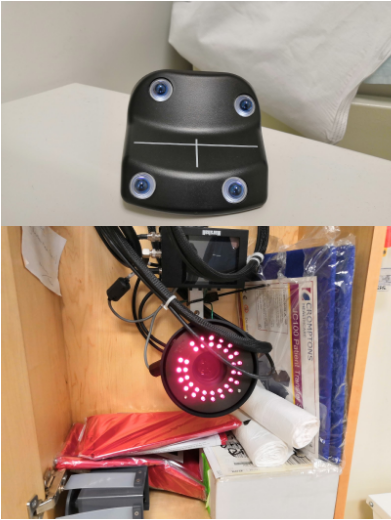
\includegraphics[width=1.0\linewidth]{figures/background_rpm.png}
                        
                    \captionsetup{singlelinecheck=false, justification=raggedright}
                    \caption{Photograph of the \gls{RPM}. On the bottom is the infrared camera and infrared \glss{LED} used to locate and track an infrared reflecting marker. On the top is the infrared reflecting marker which is placed onto the chest or stomach of the patient in order to track the respiratory amplitude of the patient. Four reflective points are used to track the marker in \gls{3D} plus a point for redundancy.} \label{fig:external_devices_rpm}
                \end{figure}
                
                \begin{figure}
                    \centering
                    
                    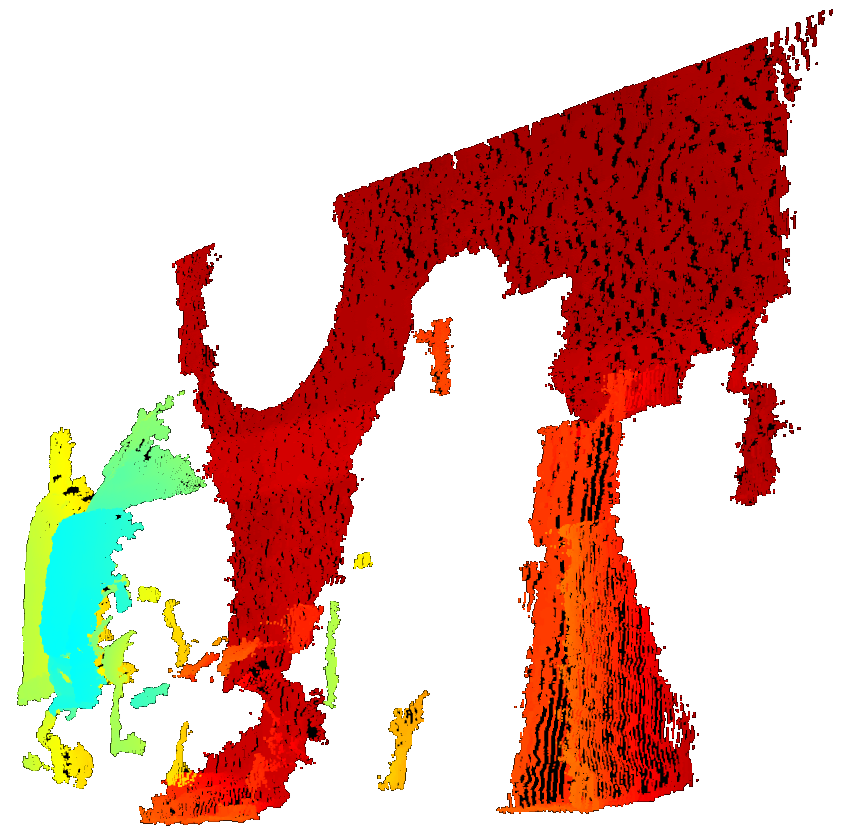
\includegraphics[width=1.0\linewidth]{figures/background_3dpc_example.png}
                    
                    \captionsetup{singlelinecheck=false, justification=raggedright}
                    \caption{Example of a \gls{3DPC} acquired on a Microsoft Kinect camera.}
                    \label{fig:external_devices_3dpc_example}
                \end{figure}
                
                There are numerous external device methods used to track the patient and acquire a \gls{SS}.  Four example devices are:
                
                \begin{itemize}
                    \item Firstly, the oldest method of \gls{SS} tracking presented here is the use of a spirometer. A spirometer is a device with a tube which is inserted into the mouth of the patient through which they breath. The spirometer measures the volume of air and the velocity with which the patient inhales or exhales~\parencite{Guivarch2004SynchronizationPlethysmography}. Some disadvantages of this method include; %that it is difficult to temporally synchronise the acquisition of the \gls{PET} data with the data from the spirometer. Additionally,
                    because spirometers are not designed for highly accurate measurement, over time, they are susceptible to value drift where the mean position of the respiratory cycle is not consistent between cycles~\parencite{Hoisak2004}.
                    
                    \item Secondly, a method borrowed from radiotherapy for \gls{SS} tracking is through the use of the Varian \gls{RPM}. The \gls{RPM} was designed to be used in radiotherapy to turn on and off the beam of a linear accelerator. This would work by using the infrared camera of the \gls{RPM} to track a reflective marker placed on the stomach or chest of the patient, tracking the displacement of the chest wall over time. This can be seen in~\Fref{fig:external_devices_rpm}. The Anzai AZ-733V system attempts to acquire the displacement of the abdomen, similarly to the \gls{RPM}, but uses a pressure belt wrapped around the patient. In radiotherapy, as the patient moves the target of the linear accelerator also moves so the beam is only turned on when the target is within a set range. In \gls{PET} the \gls{RPM} has been modified to output a clock tick to the computer acquiring the \gls{PET} data, this computer will %then synchronise with the \gls{RPM} clock and 
                    record timing information into the \gls{PET} data in order to align the \gls{RPM} \gls{SS} post acquisition. This method has the advantage over the spirometer in that it is significantly less susceptible to drift. However, the use of the \gls{RPM} increases scan time and as such receives push back from radiographers.
                    
                    \item Thirdly, optical or laser based cameras, such as the Microsoft Kinect, can be used to determine a segmentation of the patient or (using the \gls{TOF} of lasers to determine depth) a \gls{3DPC} of the patient, at each time point. An example of a \gls{3DPC} acquired on a Microsoft Kinect camera can be seen in~\Fref{fig:external_devices_3dpc_example}. A \gls{3DPC} is a collection of coordinates measured as points on the surface of the object being scanned at some displacement. A \gls{SS} can be acquired by finding the difference in these segmentations or \glss{3DPC} over time~\parencite{Miranda2017MarkerlessAnimals}. Advantages of this solution include; it doesn't make use of a reflective marker placed on the patient, like the \gls{RPM}, and as such shouldn't increase scan time. Additionally, an optical or laser based camera can track motion over a larger \gls{FOV} than the \gls{RPM}, for instance, an optical or laser based camera could conceivably simultaneously track both respiratory and head motion, producing directly a \gls{DVF} or separate \glss{SS}. A disadvantage is that it is much more difficult to spatially and temporally align the acquisition of both a \gls{PET} scanner and a stand alone optical or laser based camera~\parencite{Noonan2012AccurateKinect}~\parencite{Noonan2015RepurposingPET}~\parencite{Whitehead2018MotionPET/CT}.
                    
                    \item Finally, on \gls{MR} scanners, there is the \gls{MR} navigator. During an \gls{MR} protocol there are times when the \gls{MR}, if told to do so, can measure specific small areas of the patient's anatomy. An \gls{MR} navigator can be used to measure a pencil shaped \gls{1D} area, for instance, the position of the diaphragm or the chest wall of the patient~\parencite{Taylor1997MRAngiography}. An advantage of this is that multiple navigators can be placed to track more than one \gls{SS}. This works by looking for edges along the \gls{1D} pencil and assuming that the edge reflects the current position of the diaphragm or chest wall. An advantage of this is that it does not require any other additional equipment other than the \gls{MR} scanner and does not significantly affect scan time. A disadvantage is that it requires a \gls{MR} scanner which is not available during \gls{PET}/\gls{CT}.
                \end{itemize}
                
            \subsubsection{Data Driven} \label{sec:data_driven}
                \begin{figure}
                    \centering
                        
                    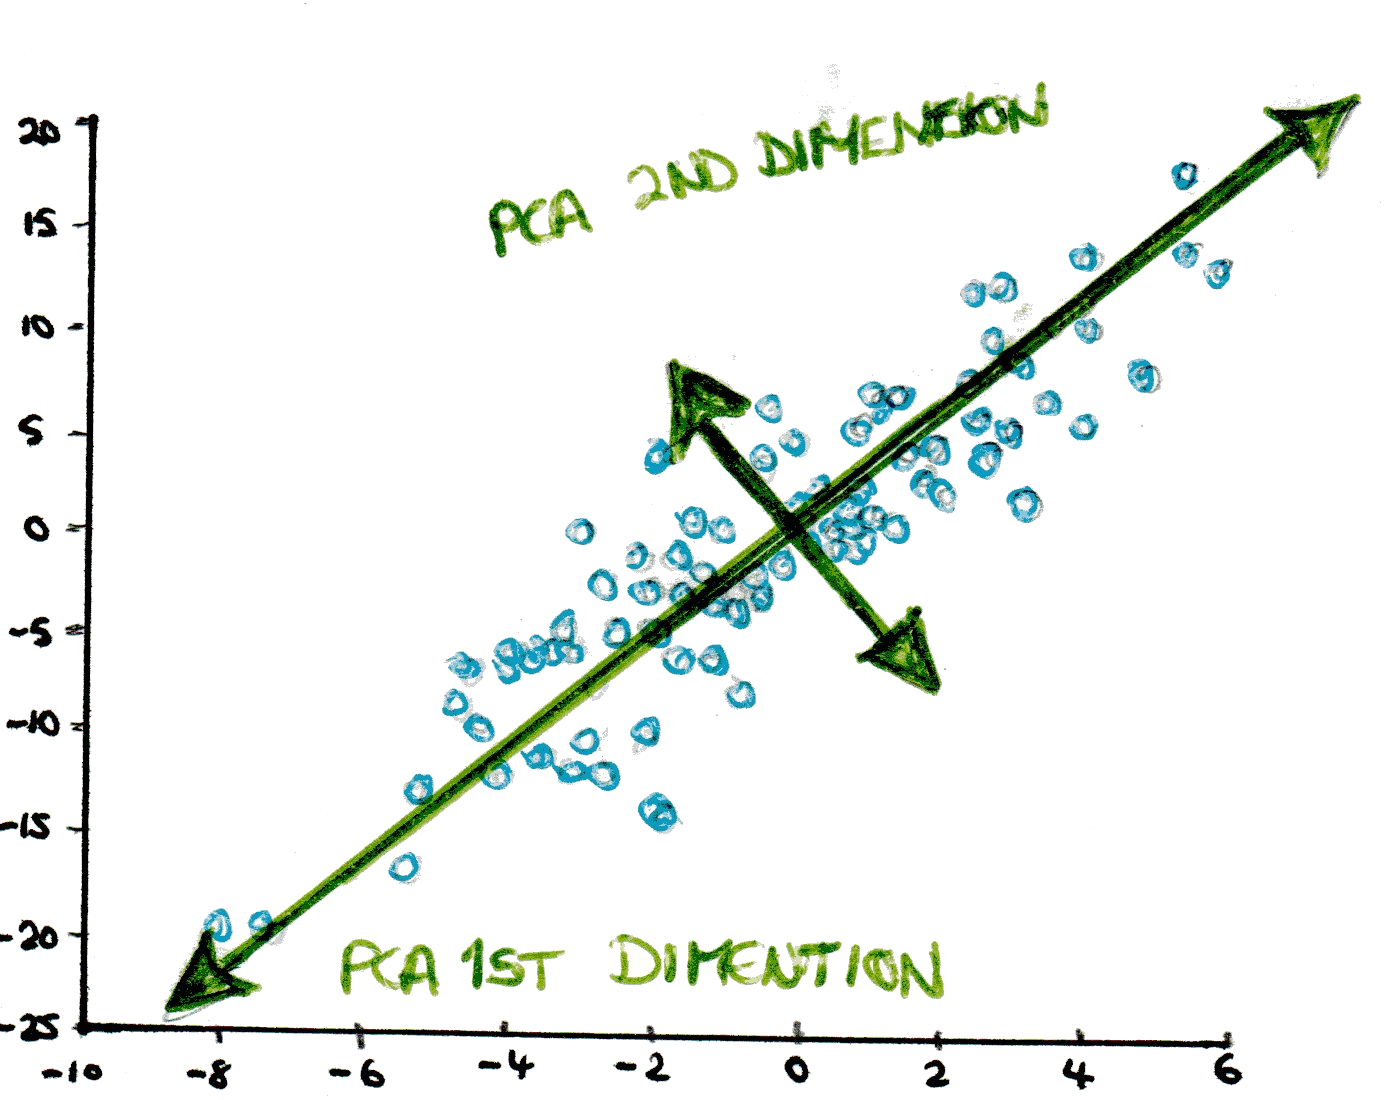
\includegraphics[width=1.0\linewidth]{figures/background_pca.png}
                        
                    \captionsetup{singlelinecheck=false, justification=raggedright}
                    \caption{Graphical representation of \gls{PCA} applied to \gls{2D} data. In the centre the \gls{2D} data points on which \gls{PCA} has been applied can be seen. From bottom left to top right the first eigenvector can be seen with most variance, from top left to bottom right the second eigenvector can be seen with less variance.} \label{fig:data_driven_pca}
                \end{figure}
                
                \begin{figure}
                    \centering
                        
                    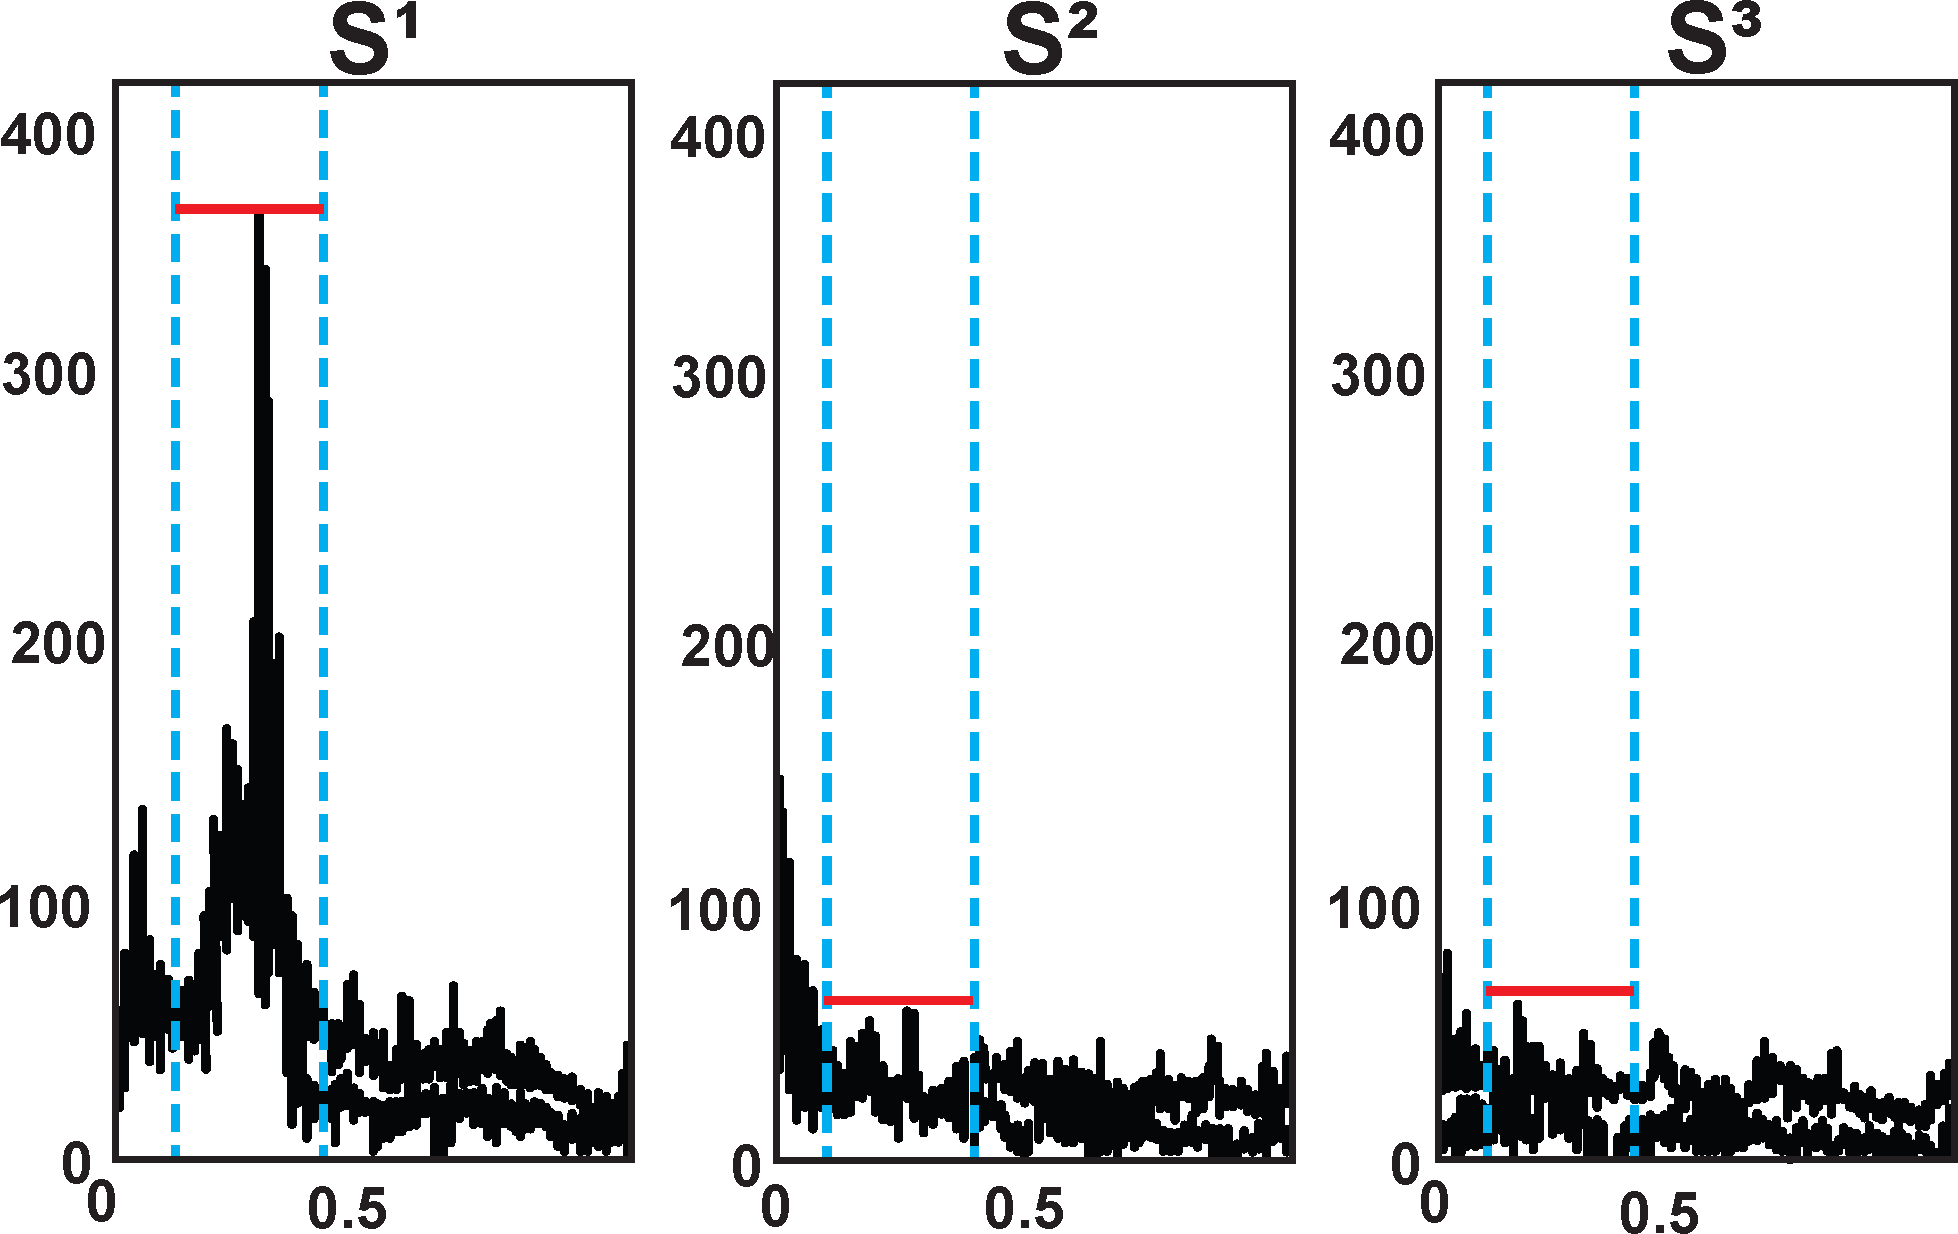
\includegraphics[width=1.0\linewidth]{figures/background_pca_window.png}
                        
                    \captionsetup{singlelinecheck=false, justification=raggedright}
                    \caption{Graphical representation of the frequency spectrum for three \gls{PC}. On the right a frequency spectrum of one \gls{PC} with a frequency window between \SI{0.1}{\hertz} and \SI{0.4}{\hertz} and a low value peak in this window can be seen. In the centre another example of what can be seen on the left can be seen. On the left another frequency spectrum with a frequency window can be seen, however, here the peak in the frequency window is significantly higher than in the other two examples.} \label{fig:data_driven_pca_window}
                \end{figure}
                
                There are numerous \gls{DD} methods used to extract a \gls{SS} directly from \gls{PET} data. Some methods require that the \gls{PET} data be reconstructed first and then markers, possibly inserted into the patient, are tracked over time. Methods requiring reconstruction are mostly inferior to methods which work on \gls{PET} acquisition data. This is because requiring that reconstruction be performed takes significant time and the \gls{SS}, itself, is usually required for most \gls{MC} methods so the initial reconstructions will be poor. Here, of the methods using \gls{PET} acquisition data, only \gls{PCA} will be discussed as it has been proven that most static \gls{DD} \gls{SS} extraction methods perform similarly~\parencite{Thielemans2013ComparisonData}. Additionally, \gls{PCA} is the method of choice on \gls{GE} scanners.
                
                \gls{PCA} is a dimensionality reduction technique, closely related to \gls{SVD}, which attempts to find a transformation that maps the data to a lower dimensional space where the underlying structure of the data can be better determined~\parencite{Pearson1901LIII.Space}. \gls{PCA} produces, for the data, a series of eigenvectors and weights where the eigenvectors (called \glss{PC}) are the orthogonal vectors of descending variance through the data (usually normalised) and the weights are the magnitude of the contribution of the components to the data, this can be seen in~\Fref{fig:data_driven_pca}. Thus the first eigenvector from \gls{PCA} will represent the vector of greatest variance through the data, in thoracic \gls{PET} this will usually be caused by the \gls{RM} of the patient, but is not always.
                
                When applied specifically to \gls{PET} acquisition data (following~\parencite{Thielemans2011}) \gls{PCA} is often used on either sinograms or unlisted listmode data, the resultant sinograms are usually spatially downsampled. This is for a number of reasons including; the noise present in the full data would obscure the motion. Additionally, the large size of the \gls{PET} sinograms provides issues when it comes to storing the number needed in memory and the computational expense necessary to apply \gls{PCA}. Furthermore, the non-downsampled sinograms contain more than enough information than is required for \gls{PCA} to be able to extract the relevant variation, thus if all the data was used then time would be wasted processing this data. Generally additional filtering (or smoothing) can be applied and in most cases will, in fact, improve results (see~\Fref{sec:pca_data_driven_surrogate_signal_extraction_methods_for_dynamic_pet_methods}). Usually when used to extract respiratory variation the sampling rate of the \gls{PET} sinograms is chosen as \SI{0.5}{\second} so as to attempt to mitigate cardiac motion by averaging most of it in each frame while still allowing for \gls{RM} between frames~\parencite{Bertolli2018Data-DrivenTomography}.
                
                The \gls{PC} which contains the variation present in the data caused by \gls{RM} must be identified. One method to do this is as follows; first, the frequency spectrum of the weight of each \gls{PC} is required, this shows at what frequency variation occurs along the weight of each \gls{PC}. Then a frequency window is determined, this is usually between \SI{0.1}{\hertz} and \SI{0.4}{\hertz} so as to coincide with the approximate frequency of respiration. The max value or peak in the frequency spectrum is then found for each \gls{PC} in this window. The \gls{PC} which has the largest peak in the window is determined as being the one best representing variance caused by \gls{RM}, this can be seen in~\Fref{fig:data_driven_pca_window}~\parencite{Thielemans2011}.
                
                Evaluations have been performed on static PET data \gls{18F-FDG} to compare the results of the \gls{DD-PCA} to both \gls{RPM} and \gls{MR} navigator based \glss{SS}. When compared to both external methods \gls{DD-PCA} was shown to be relatively robust, specifically showing a correlation of $0.89$ over nine patients when compared to the \gls{MR} navigator based \glss{SS}~\parencite{Thielemans2013ComparisonData}~\parencite{Manber2015PracticalPET/MR.}.
                
                An advantage of the \gls{PCA} based \gls{SS} extraction method (or any \gls{DD} \gls{SS} extraction method) over external device based \gls{SS} tracking is that the \gls{PCA} method allows for \gls{SS} extraction at any point during the scan, once \gls{PET} acquisition data has been acquired of the thorax, even post scan. \gls{DD-PCA} can be applied automatically without the intervention of a clinician, nor radiographer, thus not affecting acquisition time or inserting additional steps into clinical practise. \gls{DD-PCA} is also usually more comfortable for the patient as it does not involve any effort from them, in either being strapped into or otherwise having to interact with a device. This is all the while, as discussed above, providing accurate results when compared to the external devices. Additionally, \gls{DD-PCA} does not require any other modality, like \gls{MR} navigators, and as such is universally appropriate wherever \gls{PET} acquisition data is available. However, it should be noted that the \gls{SS} acquired will vary depending on the modality it is applied to, for instance, if \gls{DD-PCA} were applied to \gls{CT} data rather than \gls{PET} then the values would not be comparable.
                
                An additional issue with \gls{DD-PCA}, when applied to dynamic \gls{PET}, is that it is sensitive to dynamic radiotracer kinetics from dynamic \gls{PET} scans, as discussed in~\Fref{sec:static_and_dynamic_acquisition}. This means that while radiotracer kinetics are apparent in the data they will cause significantly more variation than \gls{RM} would do and thus mask the respiratory \gls{SS} derived via \gls{DD-PCA}. It is also not the case that the whole of the respiratory variation would be displaced to another \gls{PC}, generally its variation is mixed with the variation cause by the radiotracer kinetics and obscured. This will be investigated further in~\Fref{sec:data_driven_surrogate_signal_extraction_results}
        
        \subsection{Applying Image Registration} \label{sec:applying_image_registration}
            \begin{figure}
                \centering
                        
                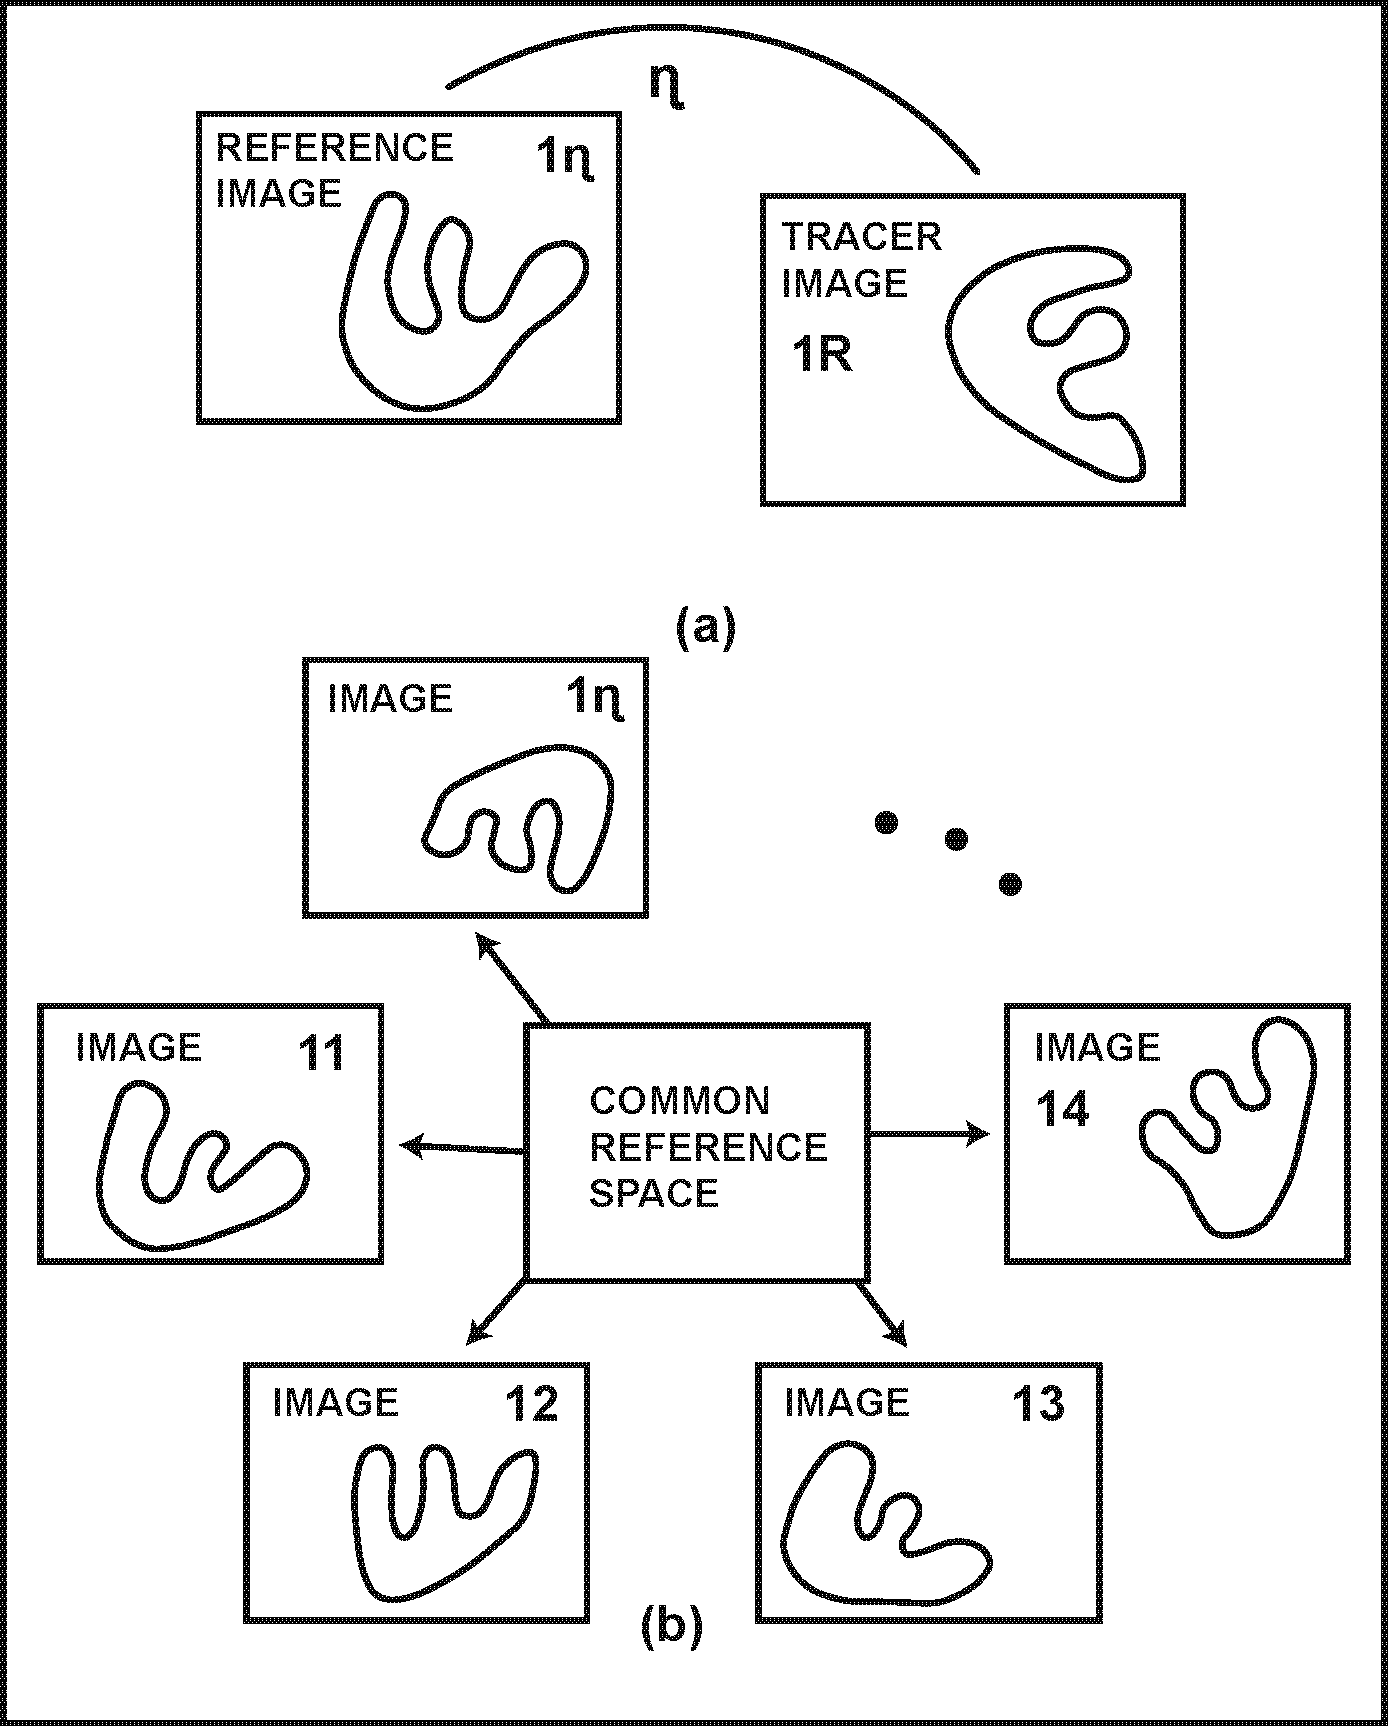
\includegraphics[width=0.9\linewidth]{figures/background_applying_image_registration_pairwise_groupwise_comparison.png}
                        
                \captionsetup{singlelinecheck=false, justification=raggedright}
                \caption{Graphical representation of the difference in methodology of pair-wise and group-wise registration. At the top of this image pair-wise registration is shown; here the target image is registered to the reference image and this process will be repeated for the number of images which are to be registered. At the bottom of the image group-wise registration is shown; here a reference common to all target images is chosen (for instance a weighted sum of the target images), this ensures the reference image is located closer to all target images than if a single target image was chosen. pair-wise registration is complete after one iteration of registration, group-wise would involve updating the common reference and registering again for a set number of iterations, as seen in~\Fref{fig:applying_image_registration_group-wise_breakdown}} \label{fig:applying_image_registration_pair-wise_group-wise_comparison}
            \end{figure}
            
            \begin{figure}
                \centering
                        
                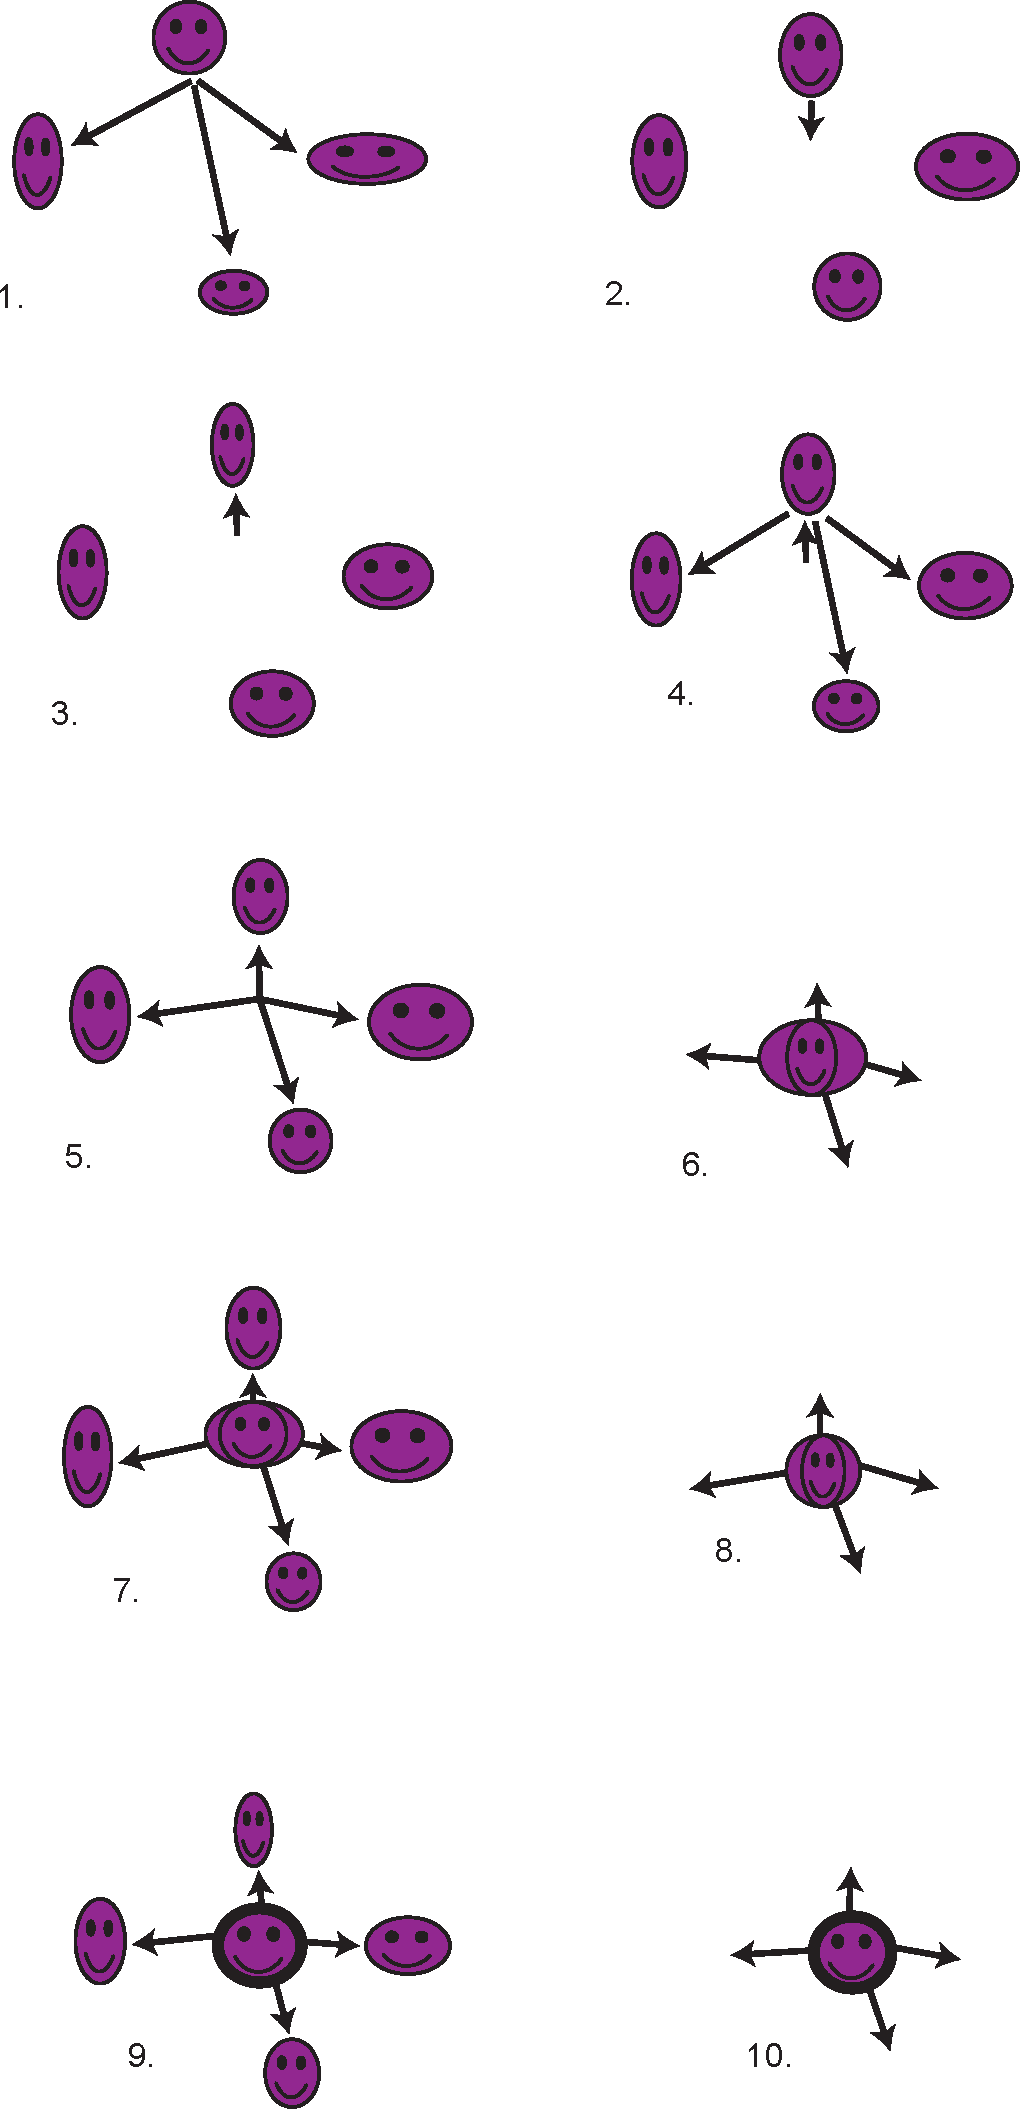
\includegraphics[width=0.5\linewidth]{figures/background_applying_image_registration_groupwise_breakdown.png}
                        
                \captionsetup{singlelinecheck=false, justification=raggedright}
                \caption{Graphical representation of one method of implementing group-wise registration. The sub-images one through four show the initial setup used for this implementation and the sub-images five through $10$ show the subsequent iterations of the group-wise algorithm. Sub-image one shows an initial pair-wise registration of one image to the rest of the images in the series. Sub-image two shows how to find the mean position of all images by taking the mean of the deformations from the previous step. Sub-image three shows the inverse of the deformation from sub-image two. Sub-image four shows the deformations from sub-image one being composed with the deformation from sub-image three, thus there is now a deformation from each image to the mean position. Sub-image five shows the resultant deformations from the composition in sub-image four. Sub-image six shows the target images resampled using the deformations from sub-image five to form a reference image at the mean position. Sub-images seven through $10$ show incremental improvements to the reference image from subsequent iterations of registration and resampling.} \label{fig:applying_image_registration_group-wise_breakdown}
            \end{figure}
            
            There are multiple ways to write an algorithm to \gls{MC} a series of respiratory gated \gls{PET} volumes incorporating \gls{IR}. Two of the most common are as follows:
            
            \begin{itemize}
                \item Firstly, pair-wise registration. Here one of the gates is selected and all other gates are registered to it. Usually the gate with the highest number of counts is selected due to it having the highest \gls{SNR}. Once \gls{IR} is complete, each gate is resampled using the corresponding \gls{DVF} and summed to form the final \gls{MCI}. An advantage of this algorithm is that it is relatively simple, usually only one pass of \gls{IR} is required and thus it could be considered relatively quick. However, the accuracy of the \gls{MC} entirely hinges on the quality of the volume selected as the reference, if it is low quality then it would be difficult to accurately register the gates. Additionally, the reference gate may be far from a number of the other gates if the reference is close to max inhalation or exhalation (compounded with a large amount of the anatomy possibly being outside the \gls{FOV} if the reference is close to max inhalation) again hindering the ease of registration.
                
                \item Secondly, group-wise registration, Here all gates are summed to form a reference volume. Gates are registered to the reference, resampled and summed once more to form a new reference volume, this process is performed a set number of times, with the quality of the reference, ideally, increasing each time. As an additional step the inverse mean of all \glss{DVF} can be composed with each \gls{DVF} before resampling the gates to ensure that the reference gate is at the mean respiratory position. A graphical representation of group-wise registration can be seen in~\Fref{fig:applying_image_registration_group-wise_breakdown}. An advantage of this algorithm is that it has the capacity to provide better registration results due to the higher \gls{SNR} of the reference volume. However, it   takes longer to perform due to the multiple full iterations of \gls{IR}.
            \end{itemize}
            
            A graphical comparison of pair-wise and group-wise registration can be seen in~\Fref{fig:applying_image_registration_pair-wise_group-wise_comparison}.
            
        \subsection{Motion Modelling} \label{sec:motion_modelling}
            \begin{figure}
                \centering
                        
                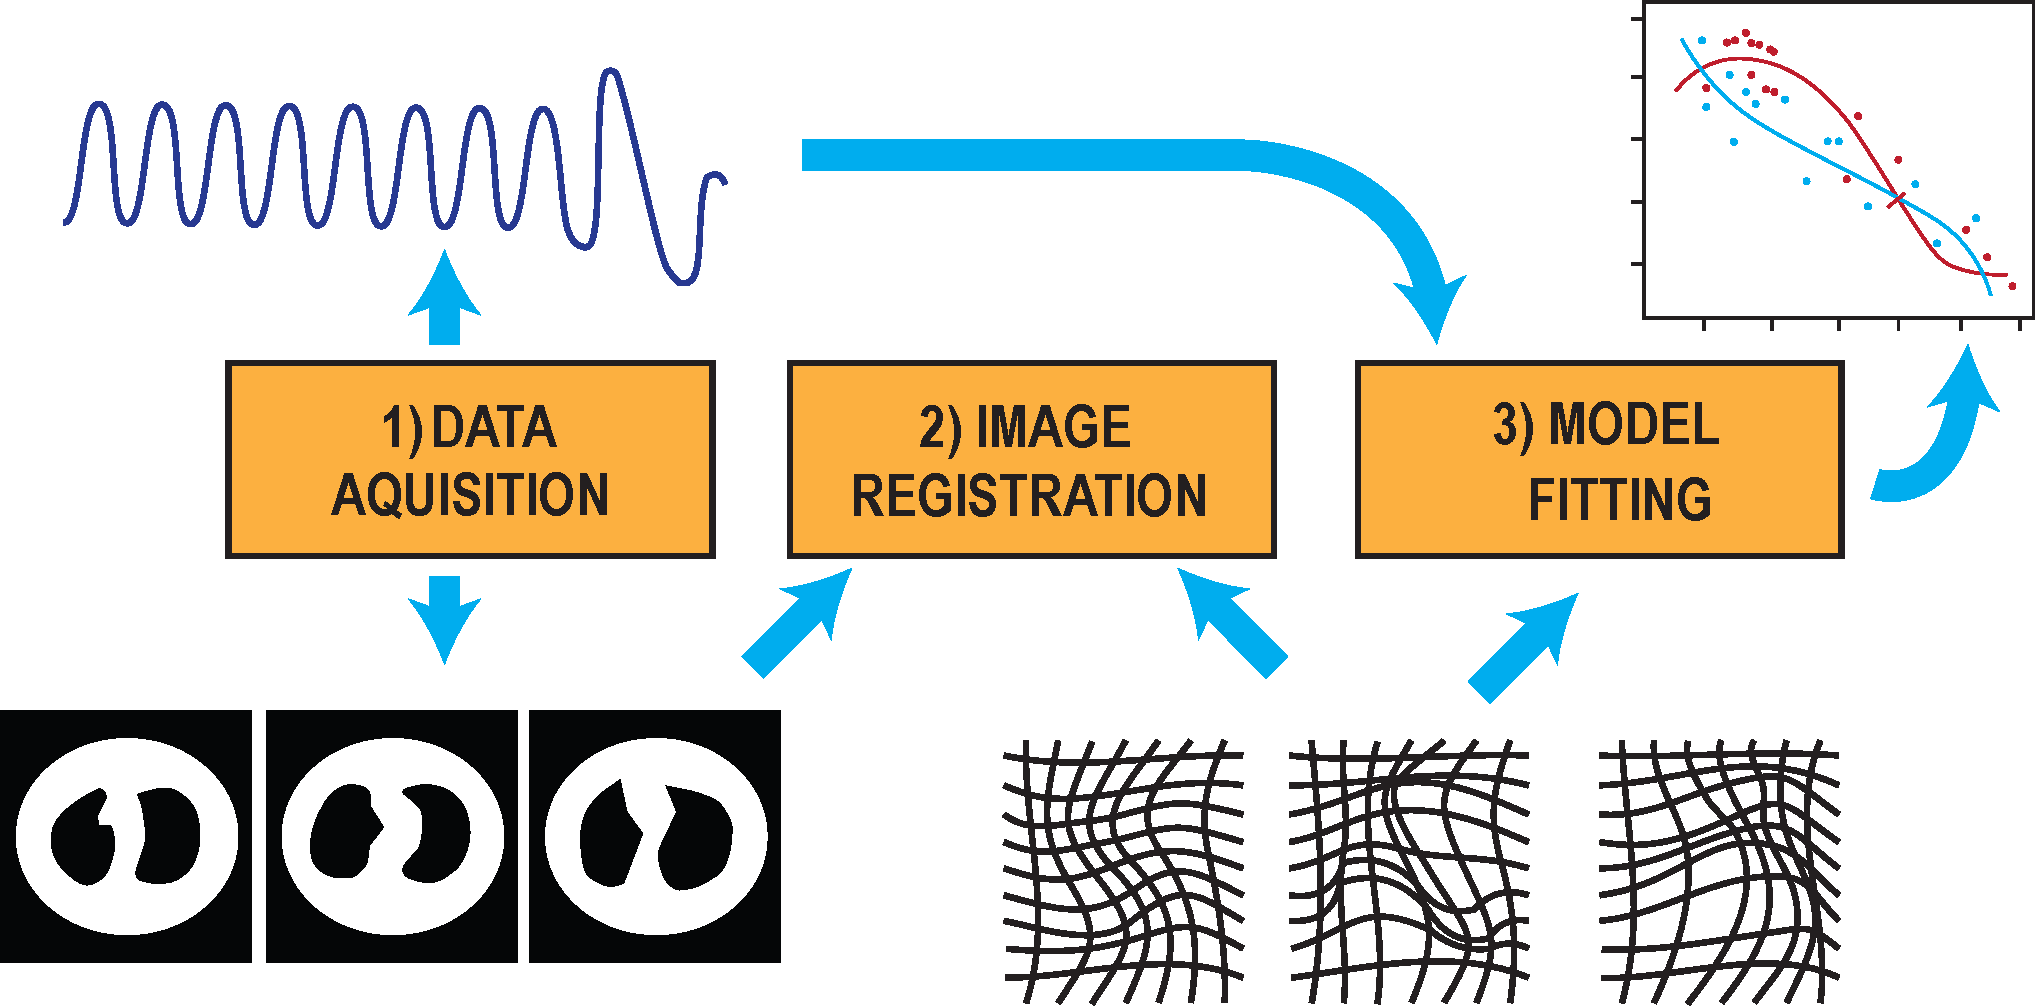
\includegraphics[width=1.0\linewidth]{figures/background_motion_model.png}
                        
                \captionsetup{singlelinecheck=false, justification=raggedright}
                \caption{Graphical representation of the process of \gls{MM}. On the left the initial data acquisition of both the data and the \gls{SS} can be seen. Then in the centre the data is taken and an \gls{IR} is applied to it. Then on the right it can be seen that the \gls{SS} is taken again and a \gls{RCM} is fit on it and the \gls{DVF} from \gls{IR}. In the top right a naive example of the \gls{2D} regression fit can be seen.} \label{fig:motion_modelling_motion_model}
            \end{figure}
            
            \glss{MM} offer an alternative solution to \gls{MC} when compared to vanilla co-registration of respiratory gated \gls{PET}. \glss{MM}, similarly to the \gls{RPM} discussed in \Fref{sec:external_devices}, is a technique borrowed from radiotherapy. \glss{MM} themselves attempt to relate the \glss{DVF} or B-spline \gls{CPG} from, for instance, \gls{IR} to the \gls{SS} acquired for the data used to generate the \glss{DVF}. In this case a \gls*{RCM} would be generated which is fit on the \glss{DVF} and \gls{SS}, this can be seen in~\Fref{fig:motion_modelling_motion_model}. In its simplest form a post \gls{IR} \gls{MM} could be a linear regression of both the \glss{DVF} and the \gls{SS}~\parencite{Kim1997MotionModel}. In the case described previously the \glss{DVF} are found first before fitting the \gls{RCM}, however, in more recent research a method to simultaneously fit both the B-spline \gls{CPG} and the \gls{RCM} has been presented~\parencite{McClelland2013}~\parencite{McClelland2006}~\parencite{McClelland2014}~\parencite{McClelland2017}. \glss{RCM} are discussed in more detail in~\Fref{sec:respiratory_correspondence_model}.
            
            There are four components required to perform \gls{MM}, these are; the data itself which is to be \gls{MC}, a \gls{SS} with an value representing the respiratory position at each data point (the \gls{SS} can be \gls{ND}), a model (such as B-spline) for the transformations and the \gls{RCM} linking the \glss{DVF} and \gls{SS}.
            
            An advantage of \gls{MM} over vanilla co-registration is that it allows for prediction of data not used to fit the \gls{RCM}. This advantage is particularly useful for radiotherapy. Here, some data is acquired on the machine used to perform radiotherapy (usually on the patient on the day of therapy). This allows for a \gls{RCM} to be fit (pre-therapy) on the data acquired with a \gls{SS} from, for instance, the \gls{RPM}. Then, as a dose is administered to the patient, from a linear accelerator, \glss{SS} values can continue to be acquired and \glss{DVF} calculated using the \gls{RCM} fit previously in order to, in real time, change the trajectory of the linear accelerator to apply a dose taking the movement into account. The new \gls{SS} values need not match any of the \gls{SS} values used to generate the \gls{RCM} as the \gls{RCM} is a continuous model. This advantage could provide the ability in \gls{PET} to calculate a \gls{RCM} while acquisition is still ongoing to be used for \gls{MC} during reconstruction (or indeed for a \gls{RCM} to be fit on a subset of the data to improve \gls{MC} speed).
            
            An additional advantage of \gls{MM} is that compared to vanilla co-registration it is more robust to noise. This is because vanilla co-registration will register each individual volume together (regardless of how well that registration fits the underlying motion of the patient) whereas \gls{MM} will then either be fit on top of (or be applied simultaneously with) registration using the \gls{SS} regularising the effect of outlying data points and noise in general.
            
            \subsubsection{Respiratory Correspondence Model} \label{sec:respiratory_correspondence_model}
                \begin{figure}
                    \centering
                            
                    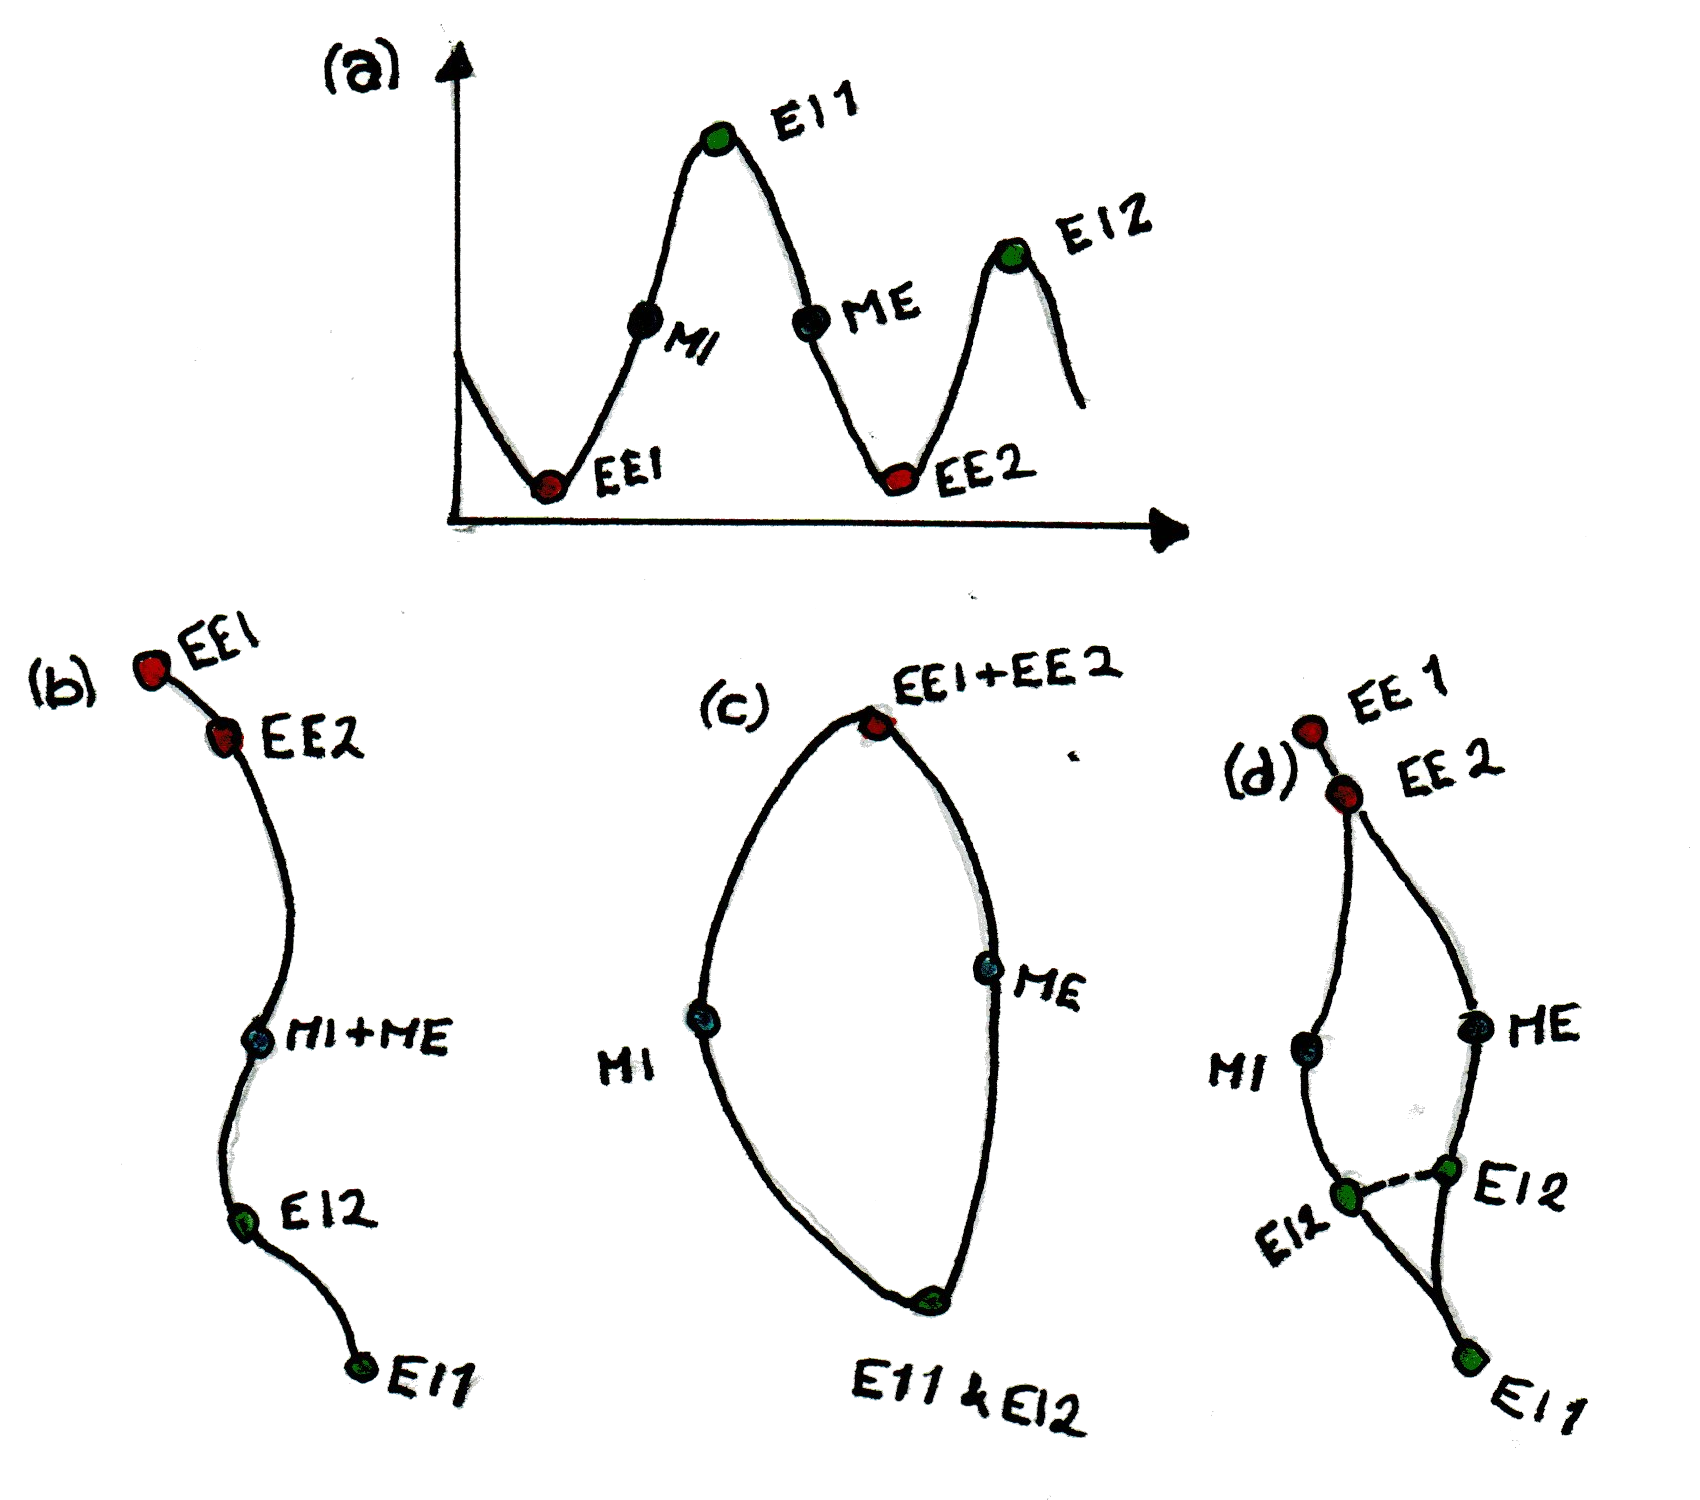
\includegraphics[width=1.0\linewidth]{figures/background_rcm.png}
                            
                    \captionsetup{singlelinecheck=false, justification=raggedright}
                    \caption{Graphical representation of the types of \gls{RCM}. At the top of the figure is a \gls{SS} which has been discretised into specific values. On the bottom left is a linear \gls{RCM}, fit on a single \gls{SS}, showing how the points from the discretised \gls{SS} would be mapped to itself. On the bottom middle is a \gls{RCM} fit on \gls{SS} reflecting the phase of the respiration and on the bottom right is an \gls{RCM} where inhalation and exhalation are modelled separately using two \gls{RCM}.} \label{fig:motion_modelling_rcm}
                \end{figure}
                
                The type of \gls{RCM} fit depends mostly upon the number and types of \gls{SS} given to the \gls{MM} algorithm and the number of models fit. Some of the different types of \gls{RCM} can be seen in~\Fref{fig:motion_modelling_rcm}. The most simple form of \gls{RCM} would be to fit a model using a single \gls{SS}, initially a \gls{SS} directly representing the amplitude of respiration, over time, could be given. A disadvantage of this approach would be that inhalation and exhalation are treated alike when in reality they differ, for instance the gradient of the \gls{SS} is not taken into account. To combat the disadvantage of the previous model a \gls{RCM} could be fit instead on the phase of respiration from the initial displacement \gls{SS}. A disadvantage of this type of \gls{RCM} is that it treats every breath as if it is exactly the same regardless of the max displacement of the breath. A final, more complex, \gls{RCM} is one where a separate model is fit for both the inhalation and exhalation portion of the data, this would mean that combined the \glss{RCM} can model both inhalation and exhalation separately, meaning that both inter- and intra-respiratory variation can be maintained. However, moving from inhalation to exhalation may incur a 'jump' in the output from the \gls{RCM}~\parencite{McClelland2013}.
                
                Furthermore, it would also be possible to fit a \gls{RCM} using more than a single \gls{SS}, for instance, one where it is fit not only on the amplitude of respiration but also the gradient of the \gls{SS}. This has the capacity to forego 'jump' issues mentioned previously while also allowing for the modelling of both inter- and intra-respiratory variation. A disadvantage of this method though is that if gating of the input data is employed then each gate would have far less data within it when compared to where a single \gls{SS} and single \gls{RCM} is used. For more detail on this final type of \gls{RCM} see~\Fref{sec:initial_motion_correction_using_basic_reconstruction_and_gating_methods_with_less_challenging_data} and~\Fref{sec:subsequent_motion_correction_using_advanced_reconstruction_and_gating_methods_with_more_challenging_data}.
                
                The reference position of the \gls{SS} with regards to the \gls{RCM} can be defined in two ways:
            
                \begin{itemize}
                    \item One, the reference position is defined as the mean respiratory position. This is similar to how the reference position is defined for group-wise registration, as discussed in~\Fref{sec:applying_image_registration}. A value of zero for the surrogate signal would correspond to the respiratory position which is in the 'centre' of all the input data or is at the mean respiratory position, i.e. it is equally 'close' to all input data.
                    
                    \item Two, if an additional dimension is added to the \gls{SS} that does not vary, it allows the intercept of the \gls{RCM} to be fit. Thus the reference position does not need to sit at the mean respiratory position, which may in some applications be useful, for instance, if the reference position was set as the position of the \gls{Mu-Map}.
                \end{itemize}
                
                As an example of fitting a \gls{RCM} using two \glss{SS}, for instance the displacement and gradient as mentioned previously. \gls{3D} B-spline can be used to model spatial deformations with the corresponding warping operation denoted as $\mathbf{W}(\mathbf{\alpha}_t)$, with $\mathbf{\alpha}_t$ a vector with B-spline coefficients at time $t$. The breathing \glss{SS} $\mathbf{s}$ containing two components. Following~\parencite{McClelland2017} a direct correspondence \gls{MM} could be used where the B-spline coefficients at time $t$ are expressed as a linear combination of the two \glss{SS}, $s_{1,t}$ and $s_{2,t}$:
            
                \begin{equation}\label{eq:respiratory_correspondence_model_motion_parameters}
                    \forall t \in [[1, n_t]], \alpha_{k, t} := R_{1, k} s_{1, t} + R_{2, k} s_{2, t} + R_{3, k}
                \end{equation}
                
                \noindent where in~\Fref{eq:respiratory_correspondence_model_motion_parameters} $\alpha_{k,t}$ is the \gls{3D} B-spline coefficient for node $k$ at time point $t$, and $R_{i,k}$ are the model parameters.
        
        \subsection{Applying Motion Correction} \label{sec:applying_motion_correction}
            As discussed throughout this chapter, in~\Fref{sec:respiratory_motion_challenges_in_combined_pet_ct_imaging} and~\Fref{sec:respiratory_gating}, there are a number of methods through which the \glss{DVF}, found from vanilla \gls{IR} or \glss{MM}, can be applied to the task of \gls{MC}. These methods mostly fit into three different classes, these are:
            
            \begin{itemize}
                \item Firstly, post reconstruction \gls{MC}. Here the \glss{DVF} are acquired and used to warp the results of \gls{PET} reconstruction once, i.e. after all iterations of the reconstruction algorithm have finished. Usually \gls{IR} is performed in image space using an objective function such as \gls{MI} or \gls{MSE}, discussed in~\Fref{sec:image_registration}. An example of a post \gls{IR} \gls{MC} technique would be performing respiratory gating, reconstructing the gated volumes and then registering and summing all gates together~\parencite{Polycarpou2012AnalysisImaging}, this was discussed briefly in~\Fref{sec:respiratory_motion_challenges_in_combined_pet_ct_imaging}. This method has the advantage that it is relatively simple to implement, each section of reconstruction and \gls{MC} is separate and sequential.
                
                \item Secondly, iterative reconstruction and \gls{MC}. This class of \gls{MC} techniques take the optimisation for reconstruction and \gls{MC} and iterates between them. An example of an iterative reconstruction and \gls{MC} technique would be \gls{ML} joint image reconstruction and motion estimation as briefly discussed in~\Fref{sec:respiratory_motion_challenges_in_combined_pet_ct_imaging}. Simply, a motion estimate for each respiratory position can be found which deforms each respiratory position to a common position~\parencite{Manjeshwar2006, Qiao2006}. However, there is additional complication in \gls{PET} caused by the \gls{Mu-Map}. Here, a \gls{ML} image reconstruction is optimised for in conjunction with a motion estimate which is applied to both the estimated activity volume and the \gls{Mu-Map}. This means that an activity volume which corresponds to the position of the \gls{Mu-Map} at every gate is found~\parencite{Bousse2016a}~\parencite{Bousse2016}. An advantage of this technique is that between every iteration, from reconstruction to \gls{MC}, the improvement of the resolution of the activity distribution aids the \gls{MC} which then in turn improve the resolution of the reconstruction. Eventually this can lead to an improved result over post reconstruction \gls{MC}. However, because this class of applied \gls{MC} involves a higher level of complexity (integrating the reconstruction and \gls{MC} algorithms) it can prove more difficult to implement and can increase computation time (due mostly to more iterations of the \gls{MC} algorithm being performed when compared to post reconstruction \gls{MC}). This class of \gls{MC} can be applied as both a deformation of the volumes as well as as adjustment to the projectors.
                
                \item Finally, there is a class of \gls{MC} method similar to the iterative reconstruction and \gls{MC} but different in that rather than independently optimising for both the motion estimation and reconstruction separately of one another they are optimised for all at once. This means the objective function of the optimisation is a combination of both the reconstruction and the motion estimation objective functions. This can be advantageous as it has been shown to give better results than optimising independently but it has the disadvantage that it introduces complexities related to the relative scale and direction of the independent terms~\parencite{Kalantari2016RespiratorySMEIR}.
            \end{itemize}
    
%    \longsection{Machine Learning for PET}{sec:machine_learning_for_pet}
        
        
%        \subsection{Machine Learning Concepts} \label{sec:machine_learning_concepts}
            
            
%            \subsubsection{Neural Network Architecture} \label{sec:neural_network_architecture}
%                \begin{figure}
%                    \centering
                            
%                    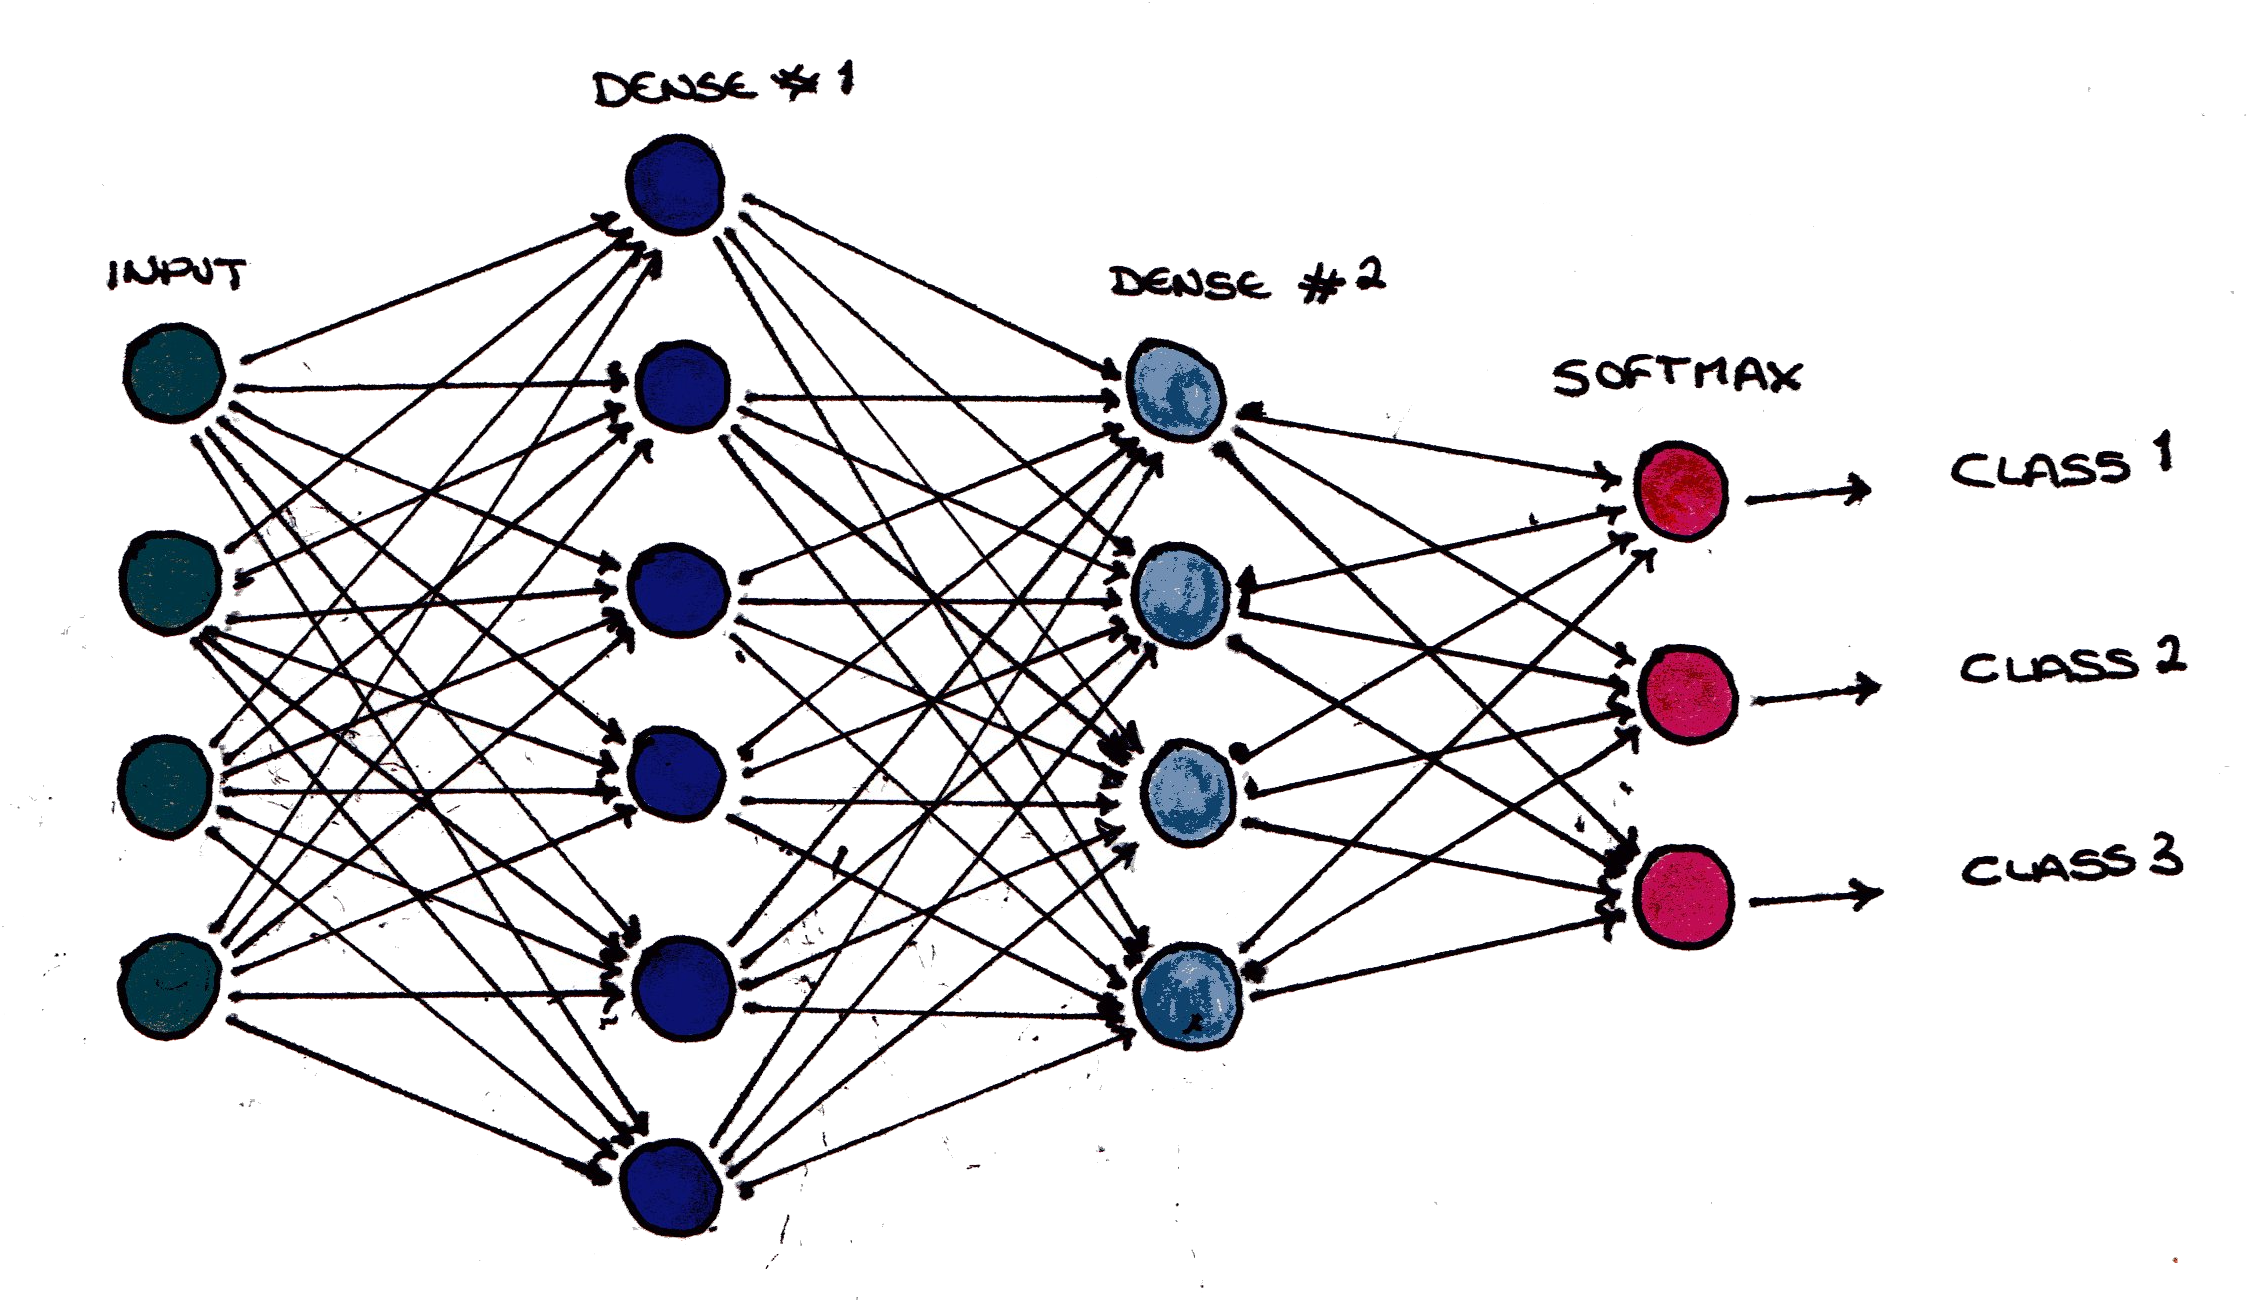
\includegraphics[width=1.0\linewidth]{figures/background_fully_connected.png}
                            
%                    \captionsetup{singlelinecheck=false, justification=raggedright}
%                    \caption{Graphical representation of . On the left .} \label{fig:neural_network_architecture_fully_connected}
%                \end{figure}
                
%                \begin{figure}
%                    \centering
                            
%                    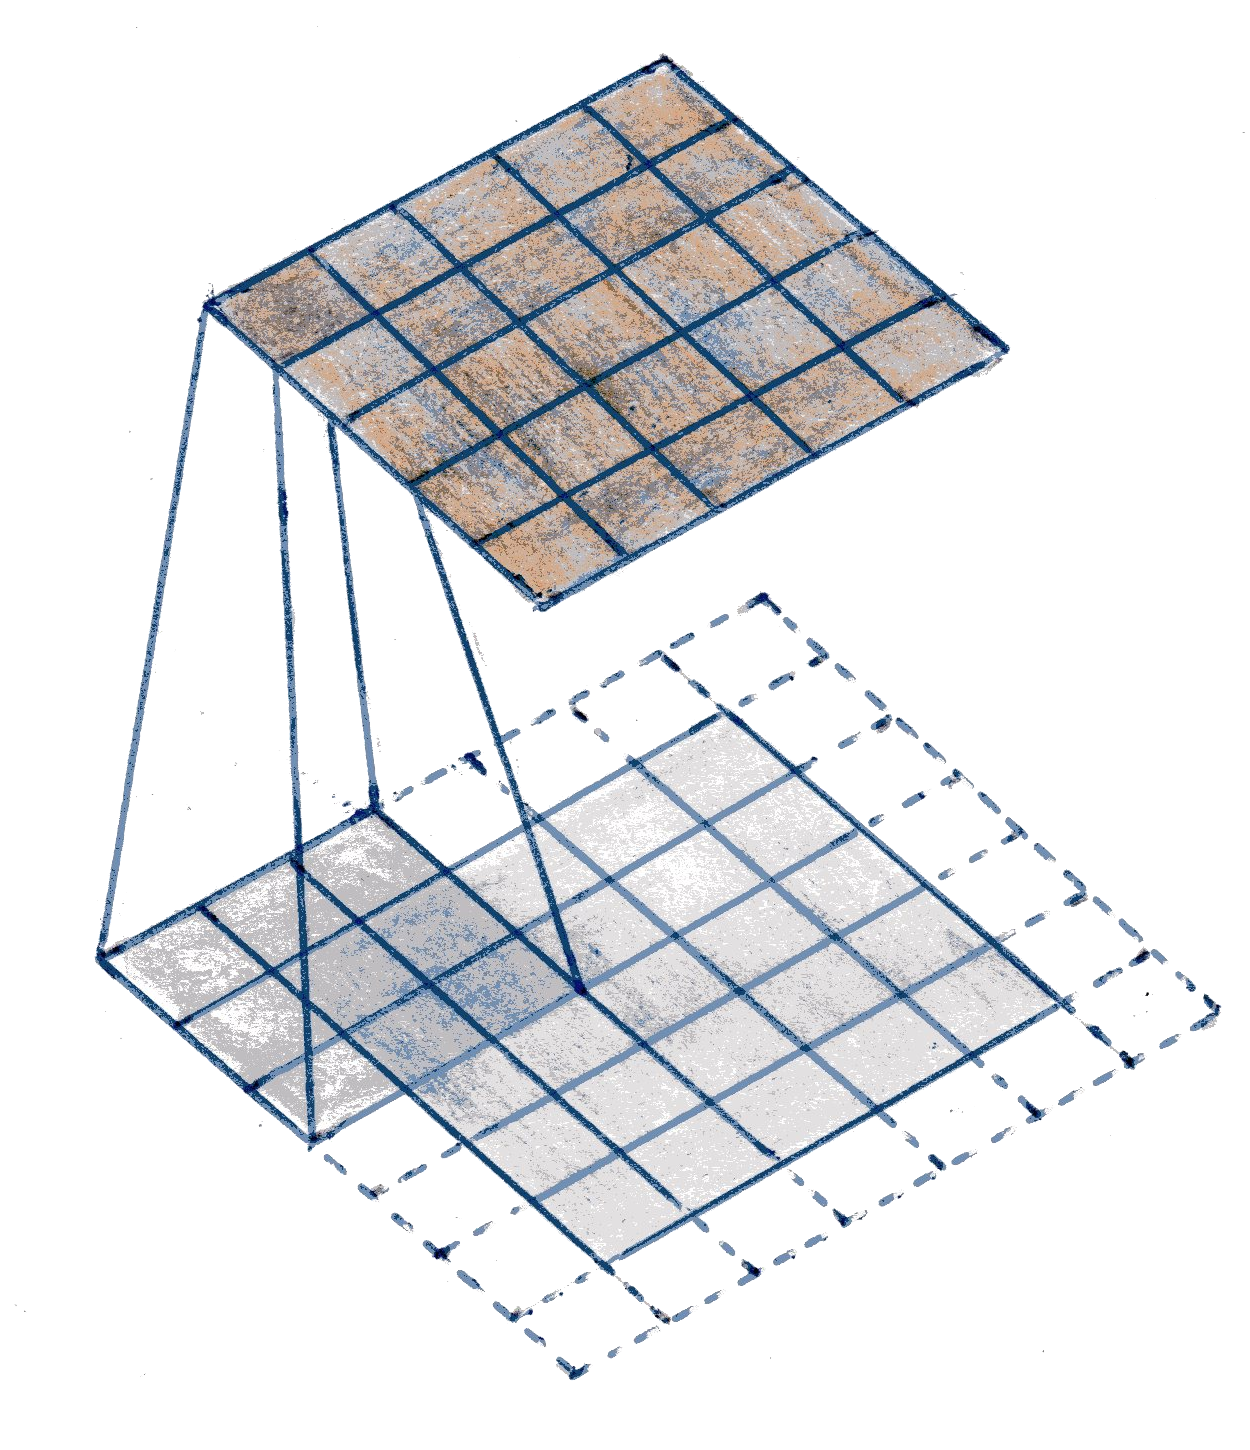
\includegraphics[width=1.0\linewidth]{figures/background_cnn.png}
                            
%                    \captionsetup{singlelinecheck=false, justification=raggedright}
%                    \caption{Graphical representation of . On the left .} \label{fig:neural_network_architecture_cnn}
%                \end{figure}
                
%                \begin{figure}
%                    \centering
                            
%                    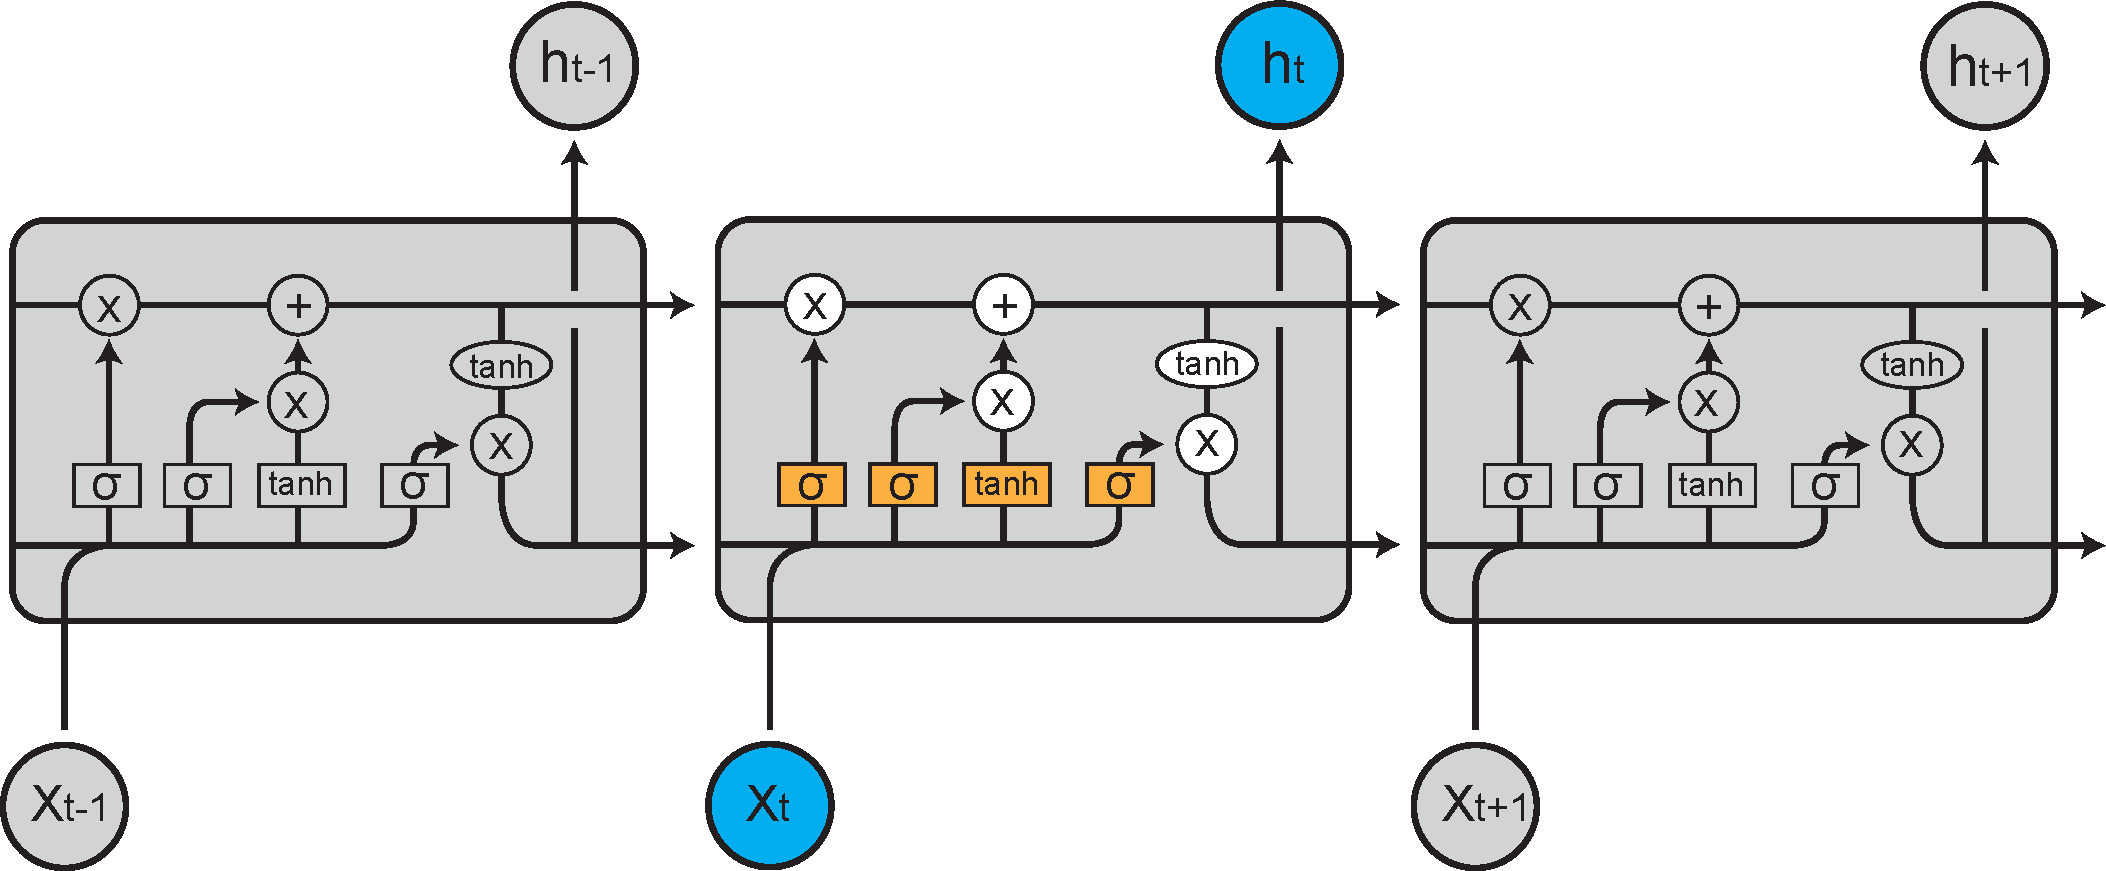
\includegraphics[width=1.0\linewidth]{figures/background_lstm.png}
                            
%                    \captionsetup{singlelinecheck=false, justification=raggedright}
%                    \caption{Graphical representation of . On the left .} \label{fig:neural_network_architecture_lstm}
%                \end{figure}
                
%            \subsubsection{Activation Function} \label{sec:activation_function}
%                \begin{figure}
%                    \centering
                            
%                    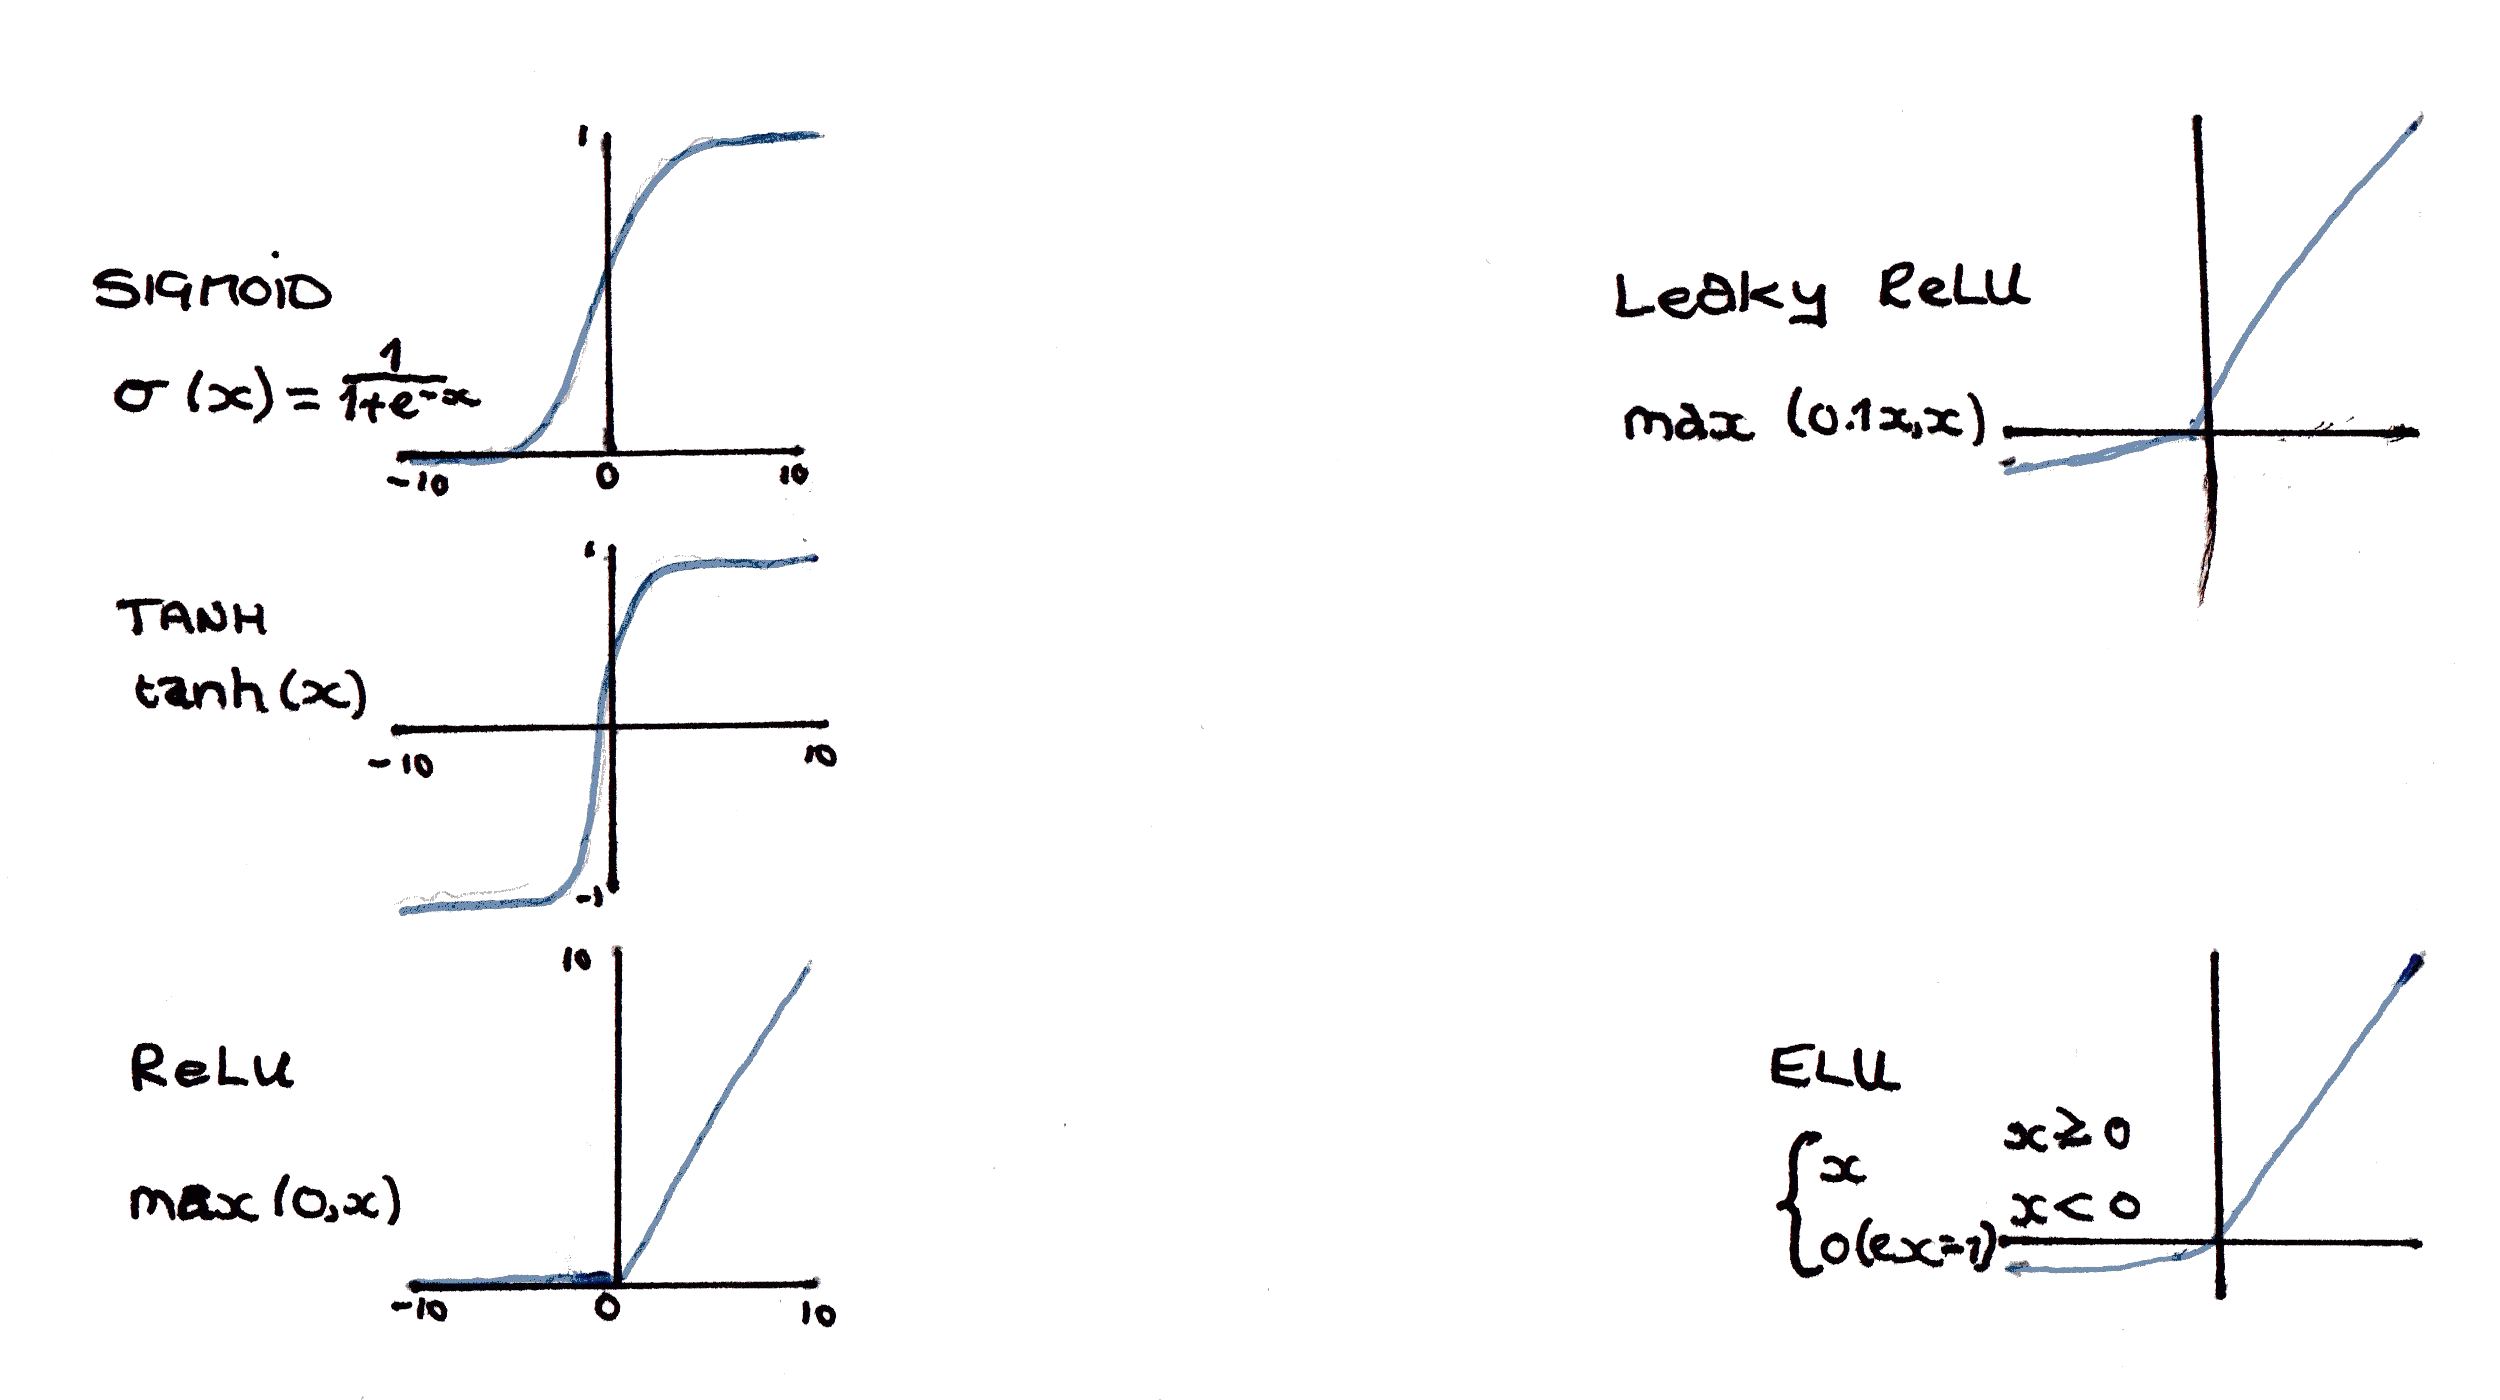
\includegraphics[width=1.0\linewidth]{figures/background_activation_functions.png}
                            
%                    \captionsetup{singlelinecheck=false, justification=raggedright}
%                    \caption{Graphical representation of . On the left .} \label{fig:activation_function_activation_functions}
%                \end{figure}
                
%                \begin{figure}
%                    \centering
                            
%                    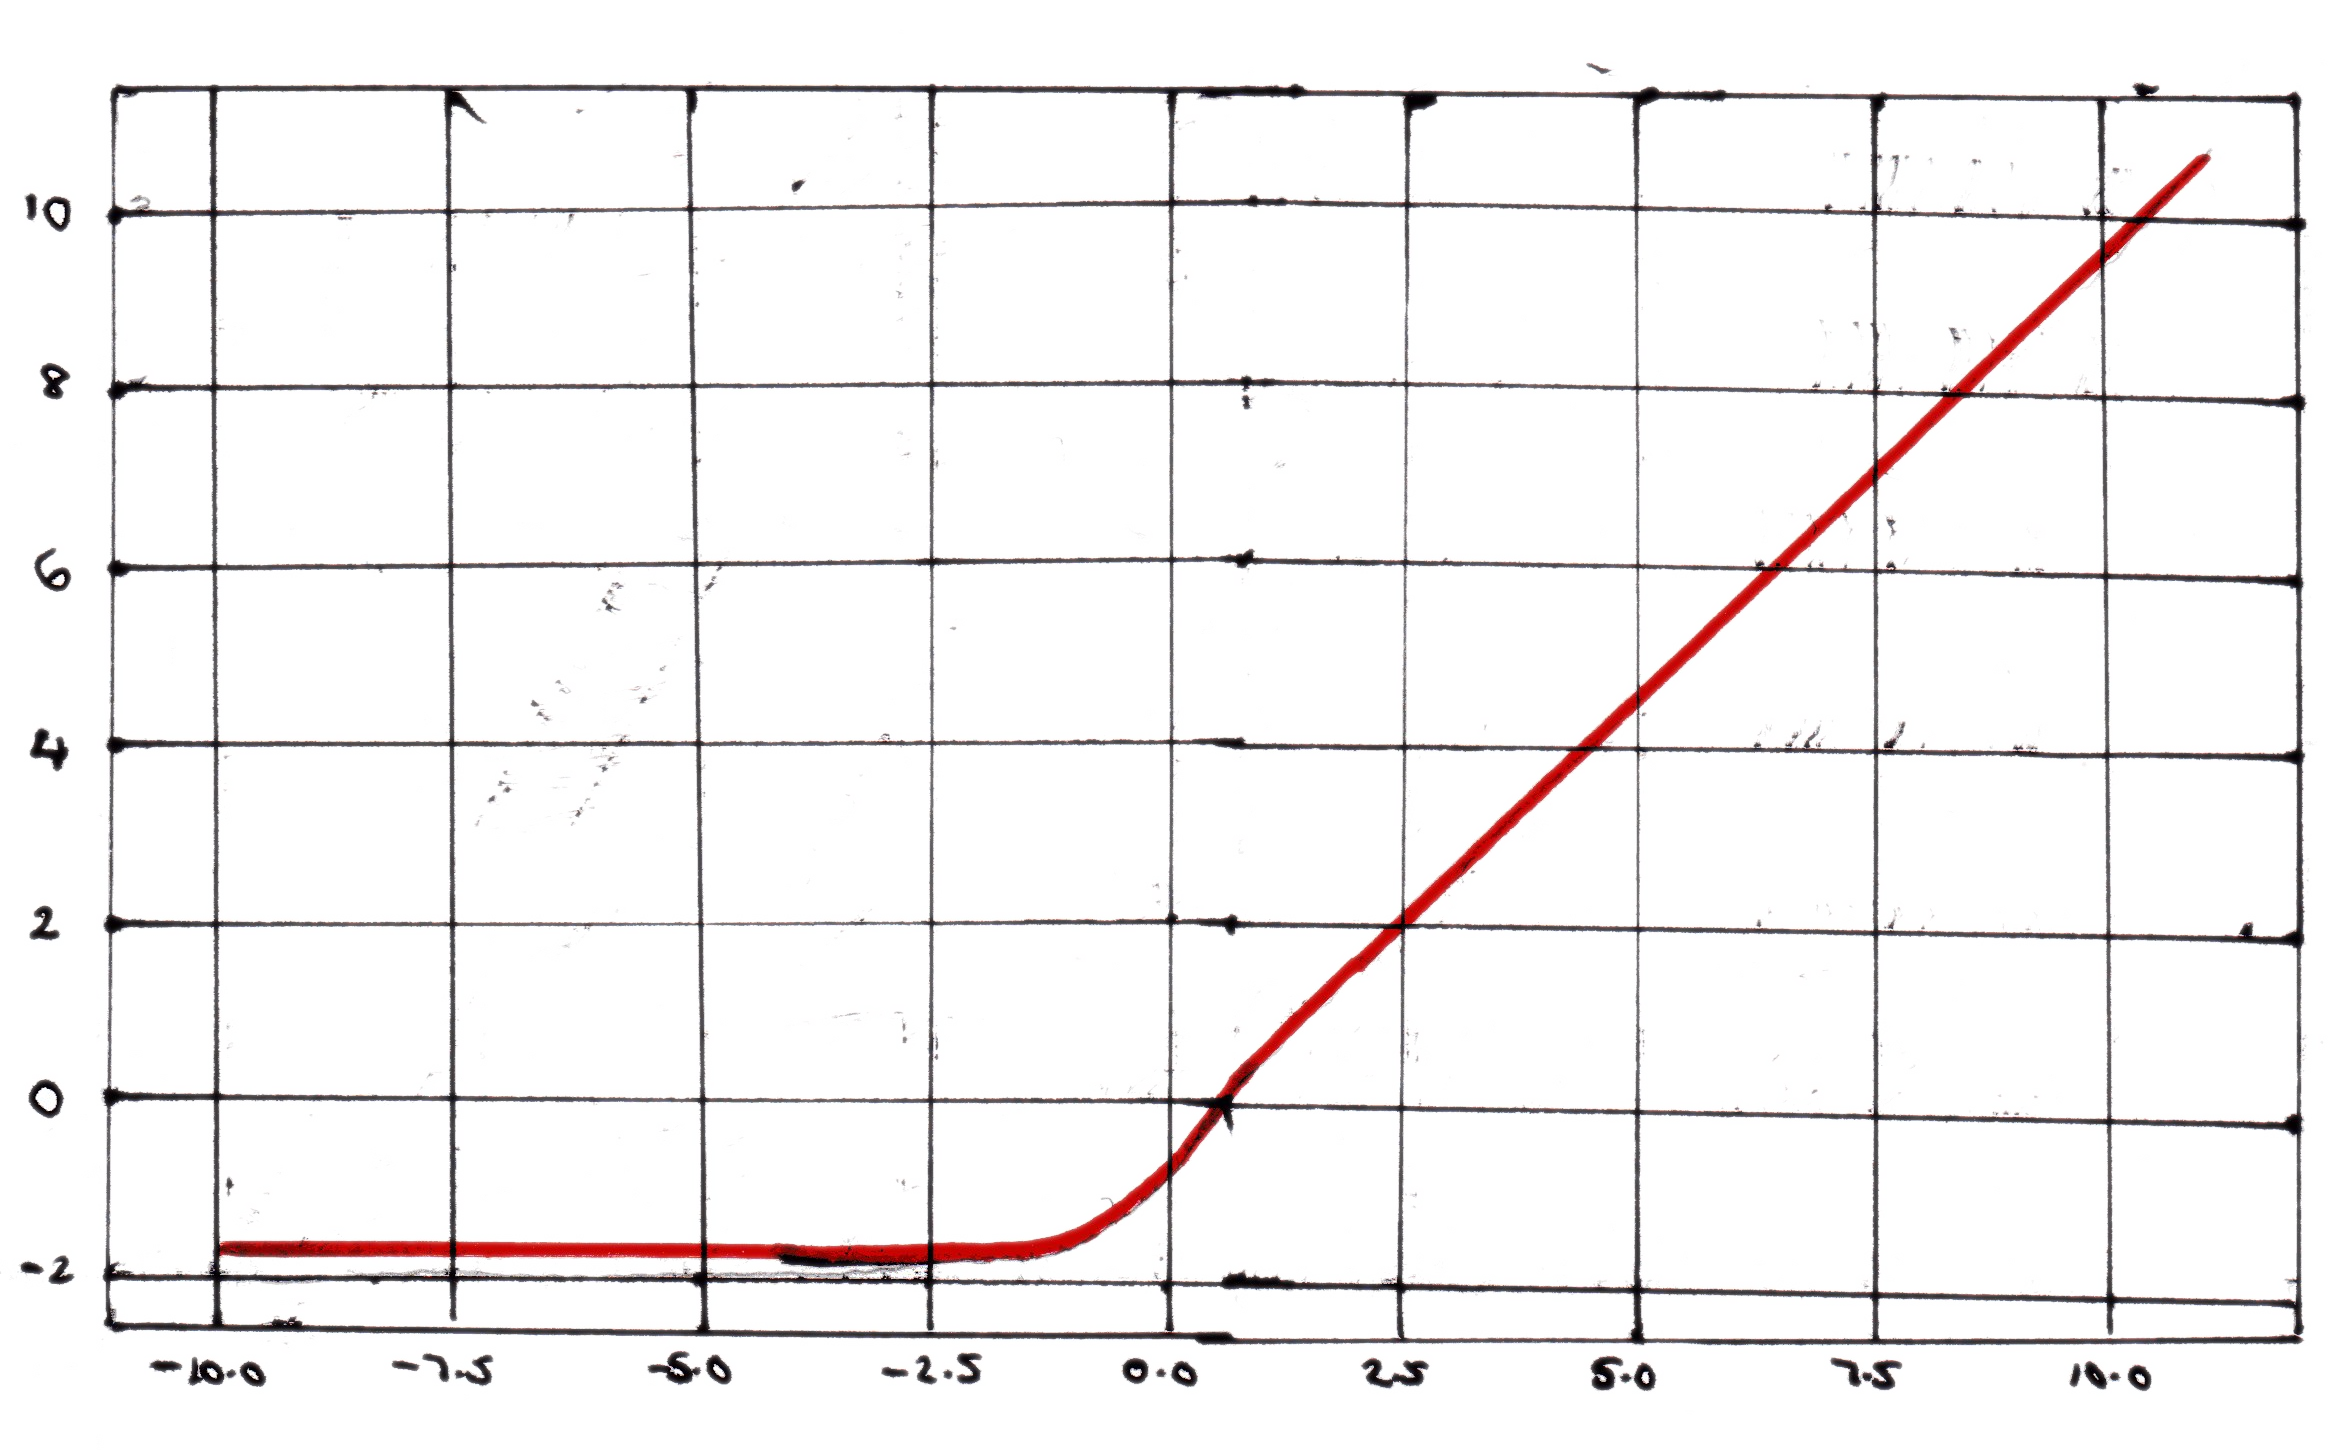
\includegraphics[width=1.0\linewidth]{figures/background_selu.png}
                            
%                    \captionsetup{singlelinecheck=false, justification=raggedright}
%                    \caption{Graphical representation of . On the left .} \label{fig:activation_function_selu}
%                \end{figure}
            
%            \subsubsection{Regularisation} \label{sec:regularisation}
%                \begin{figure}
%                    \centering
                            
%                    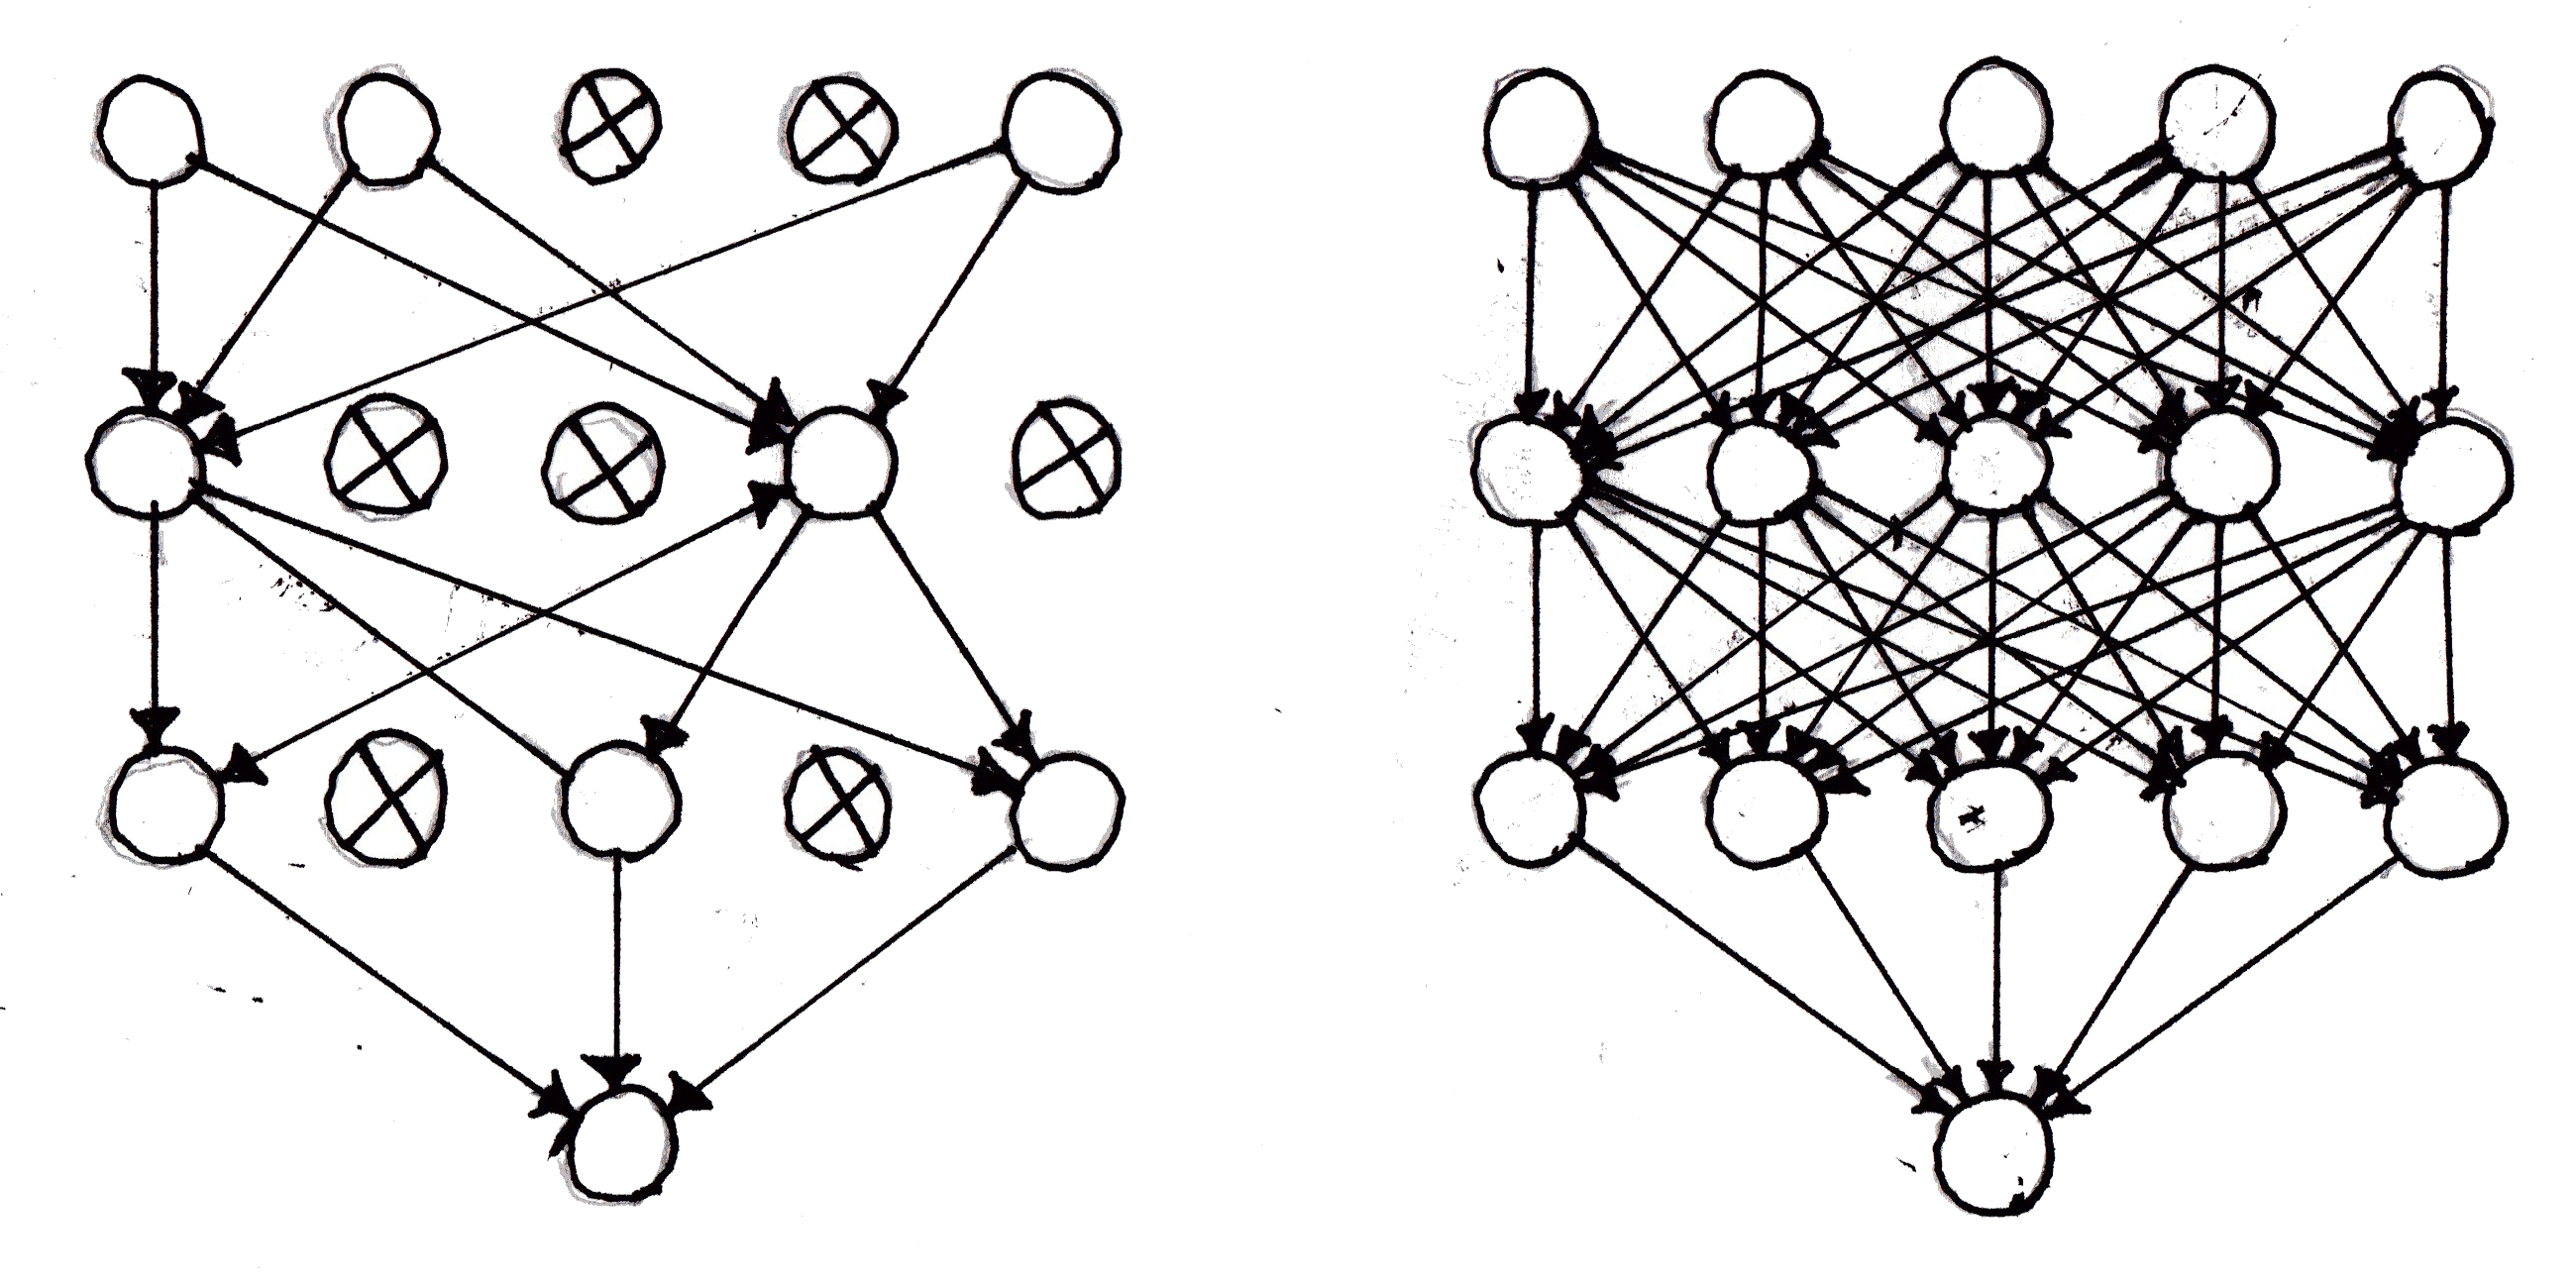
\includegraphics[width=1.0\linewidth]{figures/background_dropout.png}
                            
%                    \captionsetup{singlelinecheck=false, justification=raggedright}
%                    \caption{Graphical representation of . On the left .} \label{fig:regularisation_dropout}
%                \end{figure}
                
        
        % \subsection{Machine Learning for PET Image Reconstruction} \label{sec:machine_learning_for_pet_image_reconstruction}
            % might want to mention this?
            
        
%        \subsection{Machine Learning for Motion Correction} \label{sec:machine_learning_for_motion_correction}

    \chapter{Impact of TOF on Respiratory Motion Model Estimation Using NAC PET} \label{sec:impact_of_tof_on_respiratory_motion_model_estimation_using_nac_pet}
    \newpage
    
    \longsection{Introduction}{sec:impact_of_tof_on_respiratory_motion_model_estimation_using_nac_pet_introduction}
        This chapter of the thesis contains the work performed in the domain of \gls{MC}. The first section of this chapter introduces preliminary work on the feasibility of \gls{MC} when \gls{AC} is not applied both with and without \gls{TOF}.
        
        The second section of this chapter highlights further work to incorporate \gls{AC} into the work from the first section. Here methods to warp a single \gls{CT} derived \gls{Mu-Map} to position at each gate using a \gls{MM} are introduced. In addition, the advantage of fitting a further \gls{MM} on the newly \gls{AC} data will be evaluated.
        
        The third section of this chapter introduces a comparison between different \gls{MC} methods, both with and without \glss{MM}. Here the data used is of very low count with a \gls{Mu-Map} at end inhalation (close to a breath hold \gls{Mu-Map}).
        
        Finally, the fourth section of this chapter discusses the problems or limitations of the work performed in the previous two sections, including some possible directions in which to rectify these limitations as well as specifying where future work may take place.
    
    
    \longsection{Impact of TOF on Respiratory Motion Model Estimation Using Pre-Gated No Intra-Cycle Motion NAC PET}{sec:impact_of_tof_on_respiratory_motion_model_estimation_using_pre_gated_no_intra_cycle_motion_nac_pet}
        This section investigates the possibility of using \glss{MM} for respiratory \gls{MC} in \gls{PET}/\gls{CT}, and in particular whether incorporating \gls{TOF} information increases the accuracy of the \glss{MM} derived from \gls{NAC} reconstructed images.
        
        \subsection{Introduction} \label{sec:impact_of_tof_on_respiratory_motion_model_estimation_using_pre_gated_no_intra_cycle_motion_nac_pet_introduction}
        As discussed in~\Fref{sec:motion_modelling}, \gls{RM} reduces image quality in \gls{PET} by causing artefacts and loss of resolution in the thoracic region~\boxcite{Nehmeh2008a}. Many methods have been proposed to correct for \gls{RM}, usually involving registration between a reference volume and a set of volumes in different positions in the respiratory cycle obtained by gating~\boxcite{Oliveira2014}. However, such pair wise registration is sensitive to noise. It also does not allow prediction of the respiratory state for data not used to estimate the motion, for instance, to be used for real time \gls{MC}. \gls{SS} driven \glss{MM} attempt to overcome these deficiencies by relating the motion in the data to a number of \gls{SS} values~\boxcite{McClelland2013}. The model can output a transformation or \gls{DVF} for every value of a \gls{SS}. \glss{MM} are fit on a series of either time or gating based volumes.

        To avoid mis-registration due to attenuation mismatches, most existing methods rely on pair wise registration of \gls{NAC} \gls{PET} volumes. The benefits of using \gls{AC} \gls{PET} for \gls{IR} are unclear. If images are reconstructed using a static \gls{Mu-Map}, then artefacts caused by the misalignment between the activity distribution and the \gls{Mu-Map} would hamper \gls{IR}. It could therefore be advantageous to estimate motion on \gls{NAC} images~\boxcite{LungMotionDiaphragmBaiBib}~\boxcite{Kalantari2017AttenuationRegistration:}~\boxcite{Dawood2008RespiratoryAlgorithms}~\boxcite{Dawood2006LungImages}. However, this is a challenging problem due to the low contrast and high noise of these volumes. Contrast may be too low to fit an accurate \gls{MM} and artefacts associated with the mismatch between the acquisition data and \gls{Mu-Map} could also obscure the underlying motion if \gls{AC} is used.
        
        In the absence of \gls{TOF}, there is no information on the activity position along the \gls{LOR} and \gls{NAC} reconstructions have high intensity near the surface and low contrast in the internal part of the body. In \gls{TOF}, the time information constrains the activity position along the \gls{LOR} changing the nature and extent of the artefacts associated with \gls{NAC} \gls{PET} as well as changing noise properties~\boxcite{Ter-Pogossian1981}.
        
        The aim of this section is to investigate whether \gls{TOF} can sufficiently increase the contrast and lower the noise of \gls{NAC} images to facilitate the calculation of accurate \glss{MM}.
        
        \subsection{Methods} \label{sec:impact_of_tof_on_respiratory_motion_model_estimation_using_pre_gated_no_intra_cycle_motion_nac_pet_methods}
            \subsubsection{XCAT Image Generation} \label{sec:impact_of_tof_on_respiratory_motion_model_estimation_using_pre_gated_no_intra_cycle_motion_nac_pet_methods_xcat_image_generation}
                \gls{XCAT}~\boxcite{Segars2010} was used to generate six volumes over a \SI{5.0}{\second} second breathing cycle, as discussed in~\Fref{sec:respiratory_correspondence_model}, with one volume at full expiration at the beginning of the cycle and one volume at full expiration at the end of the cycle and using the default \gls{XCAT} settings for the extent of \gls{AP} and \gls{SI} motion (default \gls{XCAT} settings being a single orthodox breathing trace). The default \gls{XCAT} settings being a, peak to peak, \SI{2.0}{\centi\metre} \gls{RM} displacement over \SI{5.0}{\second}. Activity concentrations were derived from a static \gls{18F-FDG} patient scan. The \gls{FOV} included the base of the lungs, diaphragm and the top of the liver with a \SI{40.0}{\milli\metre} diameter spherical lesion placed in the right lung.
            
            \subsubsection{PET Data Simulation} \label{sec:impact_of_tof_on_respiratory_motion_model_estimation_using_pre_gated_no_intra_cycle_motion_nac_pet_methods_pet_data_simulation}
                \gls{PET} acquisitions were simulated using \gls{STIR}~\boxcite{Thielemans2012} through \gls{SIRF}~\boxcite{Ovtchinnikov2017} to forward project the input data to sinograms using the geometry of a \gls{GE} Discovery 690/710 and, where relevant, a \gls{TOF} resolution of \SI{375.0}{\pico\second} similar to the \gls{GE} Signa \gls{PET}/\gls{MR} (using \gls{TOF} mashing to reduce computation time resulting in $13$ \gls{TOF} time bins of size \SI{376.5}{\pico\second}). Attenuation was included in the simulation using the relevant \gls{Mu-Map} generated by \gls{XCAT}. Scatter and randoms were not taken into account in the simulation. Poisson noise realisations were generated to simulate an acquisition as if it had been gated into six bins over an acquisition of \SI{120}{\second}, emulating a standard single bed position acquisition. 
            
            \subsubsection{Image Reconstruction} \label{sec:impact_of_tof_on_respiratory_motion_model_estimation_using_pre_gated_no_intra_cycle_motion_nac_pet_methods_image_reconstruction}
                Data were reconstructed without \gls{AC} using \gls{OSEM} with two full iterations and $24$ subsets~\boxcite{Hudson1994}. Volumes were post-filtered using a \gls{3D} Gaussian blurring with a kernel size of \SI{6.4}{\milli\metre} \gls{FWHM}.
            
            \subsubsection{Motion Model Estimation} \label{sec:impact_of_tof_on_respiratory_motion_model_estimation_using_pre_gated_no_intra_cycle_motion_nac_pet_methods_motion_model_estimation}
                Following on from what is presented in~\Fref{sec:respiratory_correspondence_model} a generalised framework unifying registration and \gls{MM} estimation, NiftyRegResp, was used to estimate the \gls{RCM}. \glss{RCM} being the models fit on the acquired \gls{SS} and \glss{DVF} which, as a function can, take in a \gls{SS} value and return the \gls{DVF} which can be used to warp a volume to a reference position. Here, using \gls{SSD} as the objective function~\boxcite{McClelland2017}.
                
            \subsubsection{Evaluation} \label{sec:impact_of_tof_on_respiratory_motion_model_estimation_using_pre_gated_no_intra_cycle_motion_nac_pet_methods_evaluation}
                Three \glss{RCM} were compared: calculated from the \gls{PET} \gls{XCAT} volumes (gold standard), \gls{NTOF} \gls{NAC} reconstructions and \gls{TOF} \gls{NAC} reconstructions. To test the accuracy of the \glss{RCM}, the three models were used to warp the \gls{PET} volume generated by \gls{XCAT} at the mean breathing position, to the position at each gate. The mean breathing position \gls{XCAT} volume was generated by calculating the mean \gls{SS} value and using this as an input to \gls{XCAT}. A mean position volume was used as the \gls{RCM} was fit with this as the reference position for the \gls{SS}, as discussed in~\Fref{sec:motion_modelling}. These estimated volumes were then compared to the original \gls{XCAT} input volumes. Difference volumes were obtained by subtracting the original \gls{XCAT} volume $\mathbf{f}_t$ and warped volumes $\mathbf{W}(\alpha_t) \mathbf{f}_\mathrm{ref}$ at the same gate. \gls{MAPE} were computed from these difference images. \gls{MAPE} is expressed as:
                
                \begin{equation} \label{eq:impact_of_tof_on_respiratory_motion_model_estimation_using_pre_gated_no_intra_cycle_motion_nac_pet_methods_mape}
                   M := \frac{\frac{1}{n}\sum_{n}\mid e_n - g_n \mid}{\frac{1}{n}\sum_{n}g_n} \times 100
                \end{equation}
                
                \noindent where in~\Fref{eq:impact_of_tof_on_respiratory_motion_model_estimation_using_pre_gated_no_intra_cycle_motion_nac_pet_methods_mape} $n$ is the number of volumes, $e_n$ are the estimated volumes and $g_n$ are the \gls{GT} volumes.
                
                In addition, the \gls{COM} of the lesion was also tracked over the six gates, by warping a volume only including the lesion in the reference position as above, and then computing the \gls{COM}. The \gls{COM} along each dimension is calculated using the following equation:
                
                \begin{equation} \label{eq:impact_of_tof_on_respiratory_motion_model_estimation_using_pre_gated_no_intra_cycle_motion_nac_pet_methods_com}
                   C_{d} := \frac{1}{n}\sum_{i = 1}^{n} d_{i}
                \end{equation}
                
                \noindent where in~\Fref{eq:impact_of_tof_on_respiratory_motion_model_estimation_using_pre_gated_no_intra_cycle_motion_nac_pet_methods_com} $n$ is the number of distinct points along dimension $d_1 \dotso d_n$.
            
        \subsection{Results} \label{sec:impact_of_tof_on_respiratory_motion_model_estimation_using_pre_gated_no_intra_cycle_motion_nac_pet_results}
            \begin{figure}
                \centering
                
                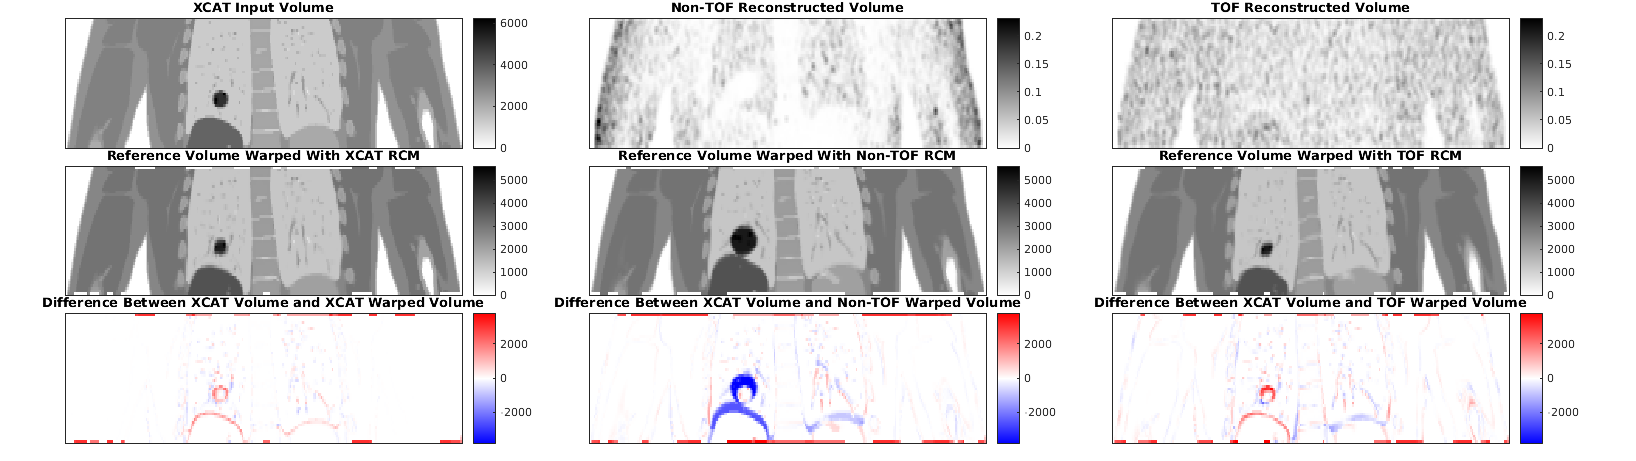
\includegraphics[width=1.0\linewidth]{figures/motion_correction_results_1_output.png}
                
                \captionsetup{singlelinecheck=false, justification=raggedright}
                \caption{All volumes correspond to end inhalation. First row from left to right: \gls{XCAT} \gls{PET} data, \gls{NAC} \gls{NTOF} reconstructed data and \gls{NAC} \gls{TOF} reconstructed data. Second row: \glss{RCM} applied to mean position \gls{XCAT} data with \glss{RCM} derived from \gls{XCAT} \gls{PET} data (left), \gls{NAC} \gls{NTOF} (middle) and \gls{NAC} \gls{TOF} (right) volumes. Colour map ranges are consistent for all images on this row. The third row from left to right:  difference between the estimated volumes from the second row with the \gls{XCAT} end inhalation volume. Colour map ranges are consistent for all images on this row.} \label{fig:impact_of_tof_on_respiratory_motion_model_estimation_using_pre_gated_no_intra_cycle_motion_nac_pet_results_output}
            \end{figure}
            
            \begin{table}
                \centering
                
                \captionsetup{singlelinecheck=false, justification=raggedright}
                \caption{Comparison of the \gls{MAPE} between the \gls{GT} data and the volumes estimated from the \gls{XCAT} based \glss{RCM}, the volumes estimated from the \gls{NAC} \gls{NTOF} based \gls{RCM} and the volumes estimated from the \gls{NAC} \gls{TOF} based \gls{RCM}.}
                
                \resizebox*{1.0\linewidth}{!}
                {
                    \begin{tabular}{||c|ccc||}
                        \hline
                        \textbf{\gls{MAPE}} & \textbf{XCAT} & \textbf{\gls{NTOF}} & \textbf{\gls{TOF}} \\
                        \hline
                        \textbf{$1$} & $1.95$ & $8.35$ & $4.18$ \\
                        \textbf{$2$} & $1.59$ & $1.61$ & $1.84$ \\
                        \textbf{$3$} & $2.06$ & $9.91$ & $5.23$ \\
                        \textbf{$4$} & $1.97$ & $6.15$ & $3.68$ \\
                        \textbf{$5$} & $1.65$ & $4.45$ & $2.52$ \\
                        \textbf{$6$} & $1.95$ & $8.35$ & $4.18$ \\
                        \hline
                        \textbf{Mean} & $1.86$ & $6.47$ & $3.60$ \\
                        \hline
                    \end{tabular}
                } \label{tab:impact_of_tof_on_respiratory_motion_model_estimation_using_pre_gated_no_intra_cycle_motion_nac_pet_results_mape}
            \end{table}
            
            \begin{figure}
                \centering
                
                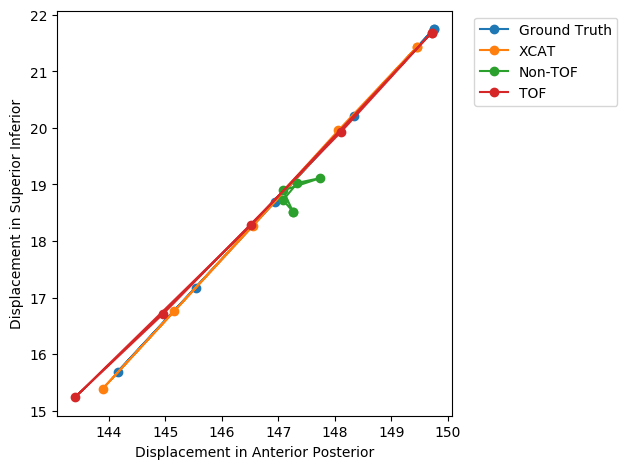
\includegraphics[width=1.0\linewidth]{figures/motion_correction_results_1_TOF.png}
                
                \captionsetup{singlelinecheck=false, justification=raggedright}
                \caption{The path of the \gls{COM} of the lesion, in voxel indices. Horizontal (respectively vertical) axis corresponds to motion in the \gls{AP} (respectively \gls{SI}) direction over the six gates. Different curves denote \gls{COM} displacement for \gls{GT} data, the estimated data from the \gls{XCAT} based \gls{RCM}, the estimated data from the \gls{NAC} \gls{NTOF} based \gls{RCM} and the estimated data from the \gls{NAC} \gls{TOF} based \gls{RCM}.} \label{fig:impact_of_tof_on_respiratory_motion_model_estimation_using_pre_gated_no_intra_cycle_motion_nac_pet_results_com_graph}
            \end{figure}
            
             The reconstructed data, estimated volumes and difference can be seen in~\Fref{fig:impact_of_tof_on_respiratory_motion_model_estimation_using_pre_gated_no_intra_cycle_motion_nac_pet_results_output} and \gls{MAPE} are in~\Fref{tab:impact_of_tof_on_respiratory_motion_model_estimation_using_pre_gated_no_intra_cycle_motion_nac_pet_results_mape}. The mean \gls{MAPE} was found to be lower for the \gls{NAC} \gls{TOF} data than for the \gls{NAC} \gls{NTOF}.
            
             \gls{COM} results can be seen in~\Fref{fig:impact_of_tof_on_respiratory_motion_model_estimation_using_pre_gated_no_intra_cycle_motion_nac_pet_results_com_graph}. The path of the \gls{NAC} \gls{TOF} data follows the \gls{GT} path much closer than the \gls{NAC} \gls{NTOF} data, and is quite close to the gold standard \gls{XCAT}-derived motion.
            
        \subsection{Conclusion} \label{sec:impact_of_tof_on_respiratory_motion_model_estimation_using_pre_gated_no_intra_cycle_motion_nac_pet_conclusion}
            \glss{MM} derived from \gls{NAC} \gls{TOF} volumes were found to be more robust than when using \gls{NAC} \gls{NTOF}, both visually and when comparing \gls{MAPE} and \gls{COM}. This was noticeable for the lung lesion in the thoracic cavity but also for other parts of the anatomy such as the liver. This is likely due to the improved image contrast of \gls{NAC} \gls{TOF} images.

            In the future, research will focus on investigating the robustness of the \gls{MM} estimation to different noise levels, acquisition duration and size of lesion. This will be expanded upon in~\Fref{sec:impact_of_tof_on_respiratory_motion_model_estimation_using_nac_pet_discussion}.
    
    \longsection{PET/CT Respiratory Motion Correction With a Single Attenuation Map Using NAC Derived Deformation Fields}{sec:pet_ct_respiratory_motion_correction_with_a_single_attenuation_map_using_nac_derived_deformation_fields}
        This section investigates the possibility of using \gls{MM} for inter-respiratory cycle \gls{MC} in \gls{PET}/\gls{CT}, and in particular whether iterative estimation of both the motion parameters and warping of a single \gls{Mu-Map}, from any respiratory position, increases the accuracy of \gls{AC} reconstruction.
        
        \subsection{Introduction} \label{sec:pet_ct_respiratory_motion_correction_with_a_single_attenuation_map_using_nac_derived_deformation_fields_introduction}
            Following on from what was presented in~\Fref{sec:impact_of_tof_on_respiratory_motion_model_estimation_using_pre_gated_no_intra_cycle_motion_nac_pet_introduction} additionally there are different strategies for handling \gls{AC} in conjunction with \gls{MC} exist. In clinical practice, usually a single \gls{Mu-Map} is available, derived from \gls{CT} in one respiratory state. This can introduce an unwanted bias (through misaligned anatomy) into the \gls{MC} algorithm. Other \gls{MC} methods can incorporate, directly, both \gls{MC} and \glss{Mu-Map} estimation into reconstruction, however, these can be computationally expensive~\boxcite{Bousse2016a}~\boxcite{Bousse2016}.
            
            This section builds upon previous work, presented in~\Fref{sec:impact_of_tof_on_respiratory_motion_model_estimation_using_pre_gated_no_intra_cycle_motion_nac_pet_methods} and evaluated in~\Fref{sec:impact_of_tof_on_respiratory_motion_model_estimation_using_pre_gated_no_intra_cycle_motion_nac_pet_results}, which suggested that \gls{NAC} data was suitable for motion estimation, through the use of \glss{MM}, if \gls{TOF} data are available. Here, the previous work is expanded upon by incorporating \gls{AC} in an iterative process. In our previous work, seen here in~\Fref{sec:impact_of_tof_on_respiratory_motion_model_estimation_using_pre_gated_no_intra_cycle_motion_nac_pet_introduction}, we investigated the possibility of using a \gls{MM} for respiratory \gls{MC} where the \gls{MM} was derived from \gls{NAC} \gls{PET}. We found that \gls{NAC} \gls{TOF} \gls{PET} was suitable to estimate the motion from gated \gls{PET} data without inter-respiratory cycle variation~\boxcite{Whitehead2019ImpactPET}. This work extends the method towards \gls{AC} with a single \gls{Mu-Map} (from any position).
        
        \subsection{Methods} \label{sec:pet_ct_respiratory_motion_correction_with_a_single_attenuation_map_using_nac_derived_deformation_fields_methods}
            \gls{NAC} are reconstructed using \gls{OSEM}, seen in~\Fref{sec:pet_ct_respiratory_motion_correction_with_a_single_attenuation_map_using_nac_derived_deformation_fields_methods_xcat_volume_generation},~\Fref{sec:pet_ct_respiratory_motion_correction_with_a_single_attenuation_map_using_nac_derived_deformation_fields_methods_pet_acquisition_simulation} and~\Fref{sec:pet_ct_respiratory_motion_correction_with_a_single_attenuation_map_using_nac_derived_deformation_fields_methods_non-attenuation_corrected_image_reconstruction}, and used as input for \gls{MM} estimation, seen in~\Fref{sec:pet_ct_respiratory_motion_correction_with_a_single_attenuation_map_using_nac_derived_deformation_fields_methods_motion_model_estimation}. A single \gls{Mu-Map} is then warped to the volumes, using the \gls{MM}, the volumes are \gls{AC}, seen in~\Fref{sec:pet_ct_respiratory_motion_correction_with_a_single_attenuation_map_using_nac_derived_deformation_fields_methods_attenuation_map_warping}, after which another motion estimation and correction cycle is performed, seen in~\Fref{sec:pet_ct_respiratory_motion_correction_with_a_single_attenuation_map_using_nac_derived_deformation_fields_methods_attenuation_corrected_image_reconstruction}.
            
            For validation, \gls{XCAT} simulations are used, for one bed position, with a \gls{FOV} including the base of the lungs and the diaphragm. The output from the proposed method is evaluated against a \gls{NMC} reconstruction of the same data visually, using a profile as well as \gls{SUV} analysis, seen in~\Fref{sec:pet_ct_respiratory_motion_correction_with_a_single_attenuation_map_using_nac_derived_deformation_fields_methods_evaluation}.
            
            \subsection{XCAT Volume Generation} \label{sec:pet_ct_respiratory_motion_correction_with_a_single_attenuation_map_using_nac_derived_deformation_fields_methods_xcat_volume_generation}
                Volume generation follows the same basic structure as presented in~\Fref{sec:impact_of_tof_on_respiratory_motion_model_estimation_using_pre_gated_no_intra_cycle_motion_nac_pet_methods_xcat_image_generation}, however here $240$ volumes were generated over a \SI{120}{\second} respiratory trace (with inter-respiratory cycle variation) derived from data captured using a \gls{RPM}. The max displacement of \gls{AP} and \gls{SI} motion was set to \SI{1.2}{\centi\metre} and \SI{2.0}{\centi\metre} respectively. The \gls{FOV} included the base of the lungs, diaphragm and the top of the liver with a \SI{20}{\milli\metre} diameter spherical lesion placed into the centre of the right lung.
    
            \subsection{PET Acquisition Simulation} \label{sec:pet_ct_respiratory_motion_correction_with_a_single_attenuation_map_using_nac_derived_deformation_fields_methods_pet_acquisition_simulation}
                Again as in~\Fref{sec:impact_of_tof_on_respiratory_motion_model_estimation_using_pre_gated_no_intra_cycle_motion_nac_pet_methods_pet_data_simulation} \gls{PET} simulation (and reconstructed) followed the same basic structure, using \gls{STIR}~\boxcite{Thielemans2012}~\boxcite{Nikos2019}~\boxcite{Wadhwa2020PETLibrary} through the \gls{SIRF}~\boxcite{Ovtchinnikov2017}, to forward project data using the geometry of a \gls{GE} Discovery $710$, but using a \gls{TOF} resolution of \SI{375}{\pico\second}. This \gls{TOF} resolution is higher than that of the $710$, but is closer to the newer \gls{GE} Signa \gls{PET}/\gls{MR} system. \gls{TOF} mashing was used to reduce computation time resulting in $13$ \gls{TOF} bins of size \SI{376.5}{\pico\second}. Multiple noise realisations were generated to simulate an acquisition over \SI{120}{\second}, emulating a standard single bed position acquisition. A respiratory \gls{SS} was generated using \gls{PCA}~\boxcite{Thielemans2011}, for more information see~\Fref{sec:respiratory_signal_detection}. This was used to gate the data into $10$ respiratory bins using displacement gating. For the purpose of the \gls{MM} fitting, \gls{SS} values were ascertained for the post-gated data by taking an average of the \gls{SS} values of the data in each bin.
            
            \subsection{Non-Attenuation Corrected Image Reconstruction} \label{sec:pet_ct_respiratory_motion_correction_with_a_single_attenuation_map_using_nac_derived_deformation_fields_methods_non-attenuation_corrected_image_reconstruction}
                Data were reconstructed without \gls{AC} using \gls{OSEM} with two full iterations and $24$ subsets~\boxcite{Hudson1994}.
                Volumes were post-filtered using a \gls{3D} Gaussian blur with a kernel size of \SI{6.4}{\milli\metre} full width half maximum.
            
            \subsection{Motion Model Estimation} \label{sec:pet_ct_respiratory_motion_correction_with_a_single_attenuation_map_using_nac_derived_deformation_fields_methods_motion_model_estimation}
                Following on from what is presented in~\Fref{sec:respiratory_correspondence_model} and~\Fref{sec:impact_of_tof_on_respiratory_motion_model_estimation_using_pre_gated_no_intra_cycle_motion_nac_pet_methods_motion_model_estimation} a generalised framework unifying \gls{IR} and respiratory \glss{MM} were used to estimate \glss{MM} and \glss{MCI}~\boxcite{McClelland2017}. \gls{SSD} was used as the similarity measure and \gls{BE} was used as a penalty. The \gls{CPG} spacing and penalty weight were tuned using a grid search.
            
            \subsection{Attenuation Map Warping} \label{sec:pet_ct_respiratory_motion_correction_with_a_single_attenuation_map_using_nac_derived_deformation_fields_methods_attenuation_map_warping}
                A \gls{Mu-Map} close to the mean respiratory position was selected from the \glss{Mu-Map} generated by \gls{XCAT}. This \gls{Mu-Map} was then registered (using \gls{NMI}) to the mean position \gls{NAC} \gls*{MCI} generated using the \gls{MM}. The \gls{MM} was then used to generate \glss{DVF} for the \gls{SS} values of each bin, which were then used to warp the \gls{Mu-Map} from the mean respiratory position to each bin.
            
            \subsection{Motion Corrected Image Reconstruction with AC} \label{sec:pet_ct_respiratory_motion_correction_with_a_single_attenuation_map_using_nac_derived_deformation_fields_methods_attenuation_corrected_image_reconstruction}
                Data were re-reconstructed, with \gls{AC}, using the \glss{Mu-Map} from~\Fref{sec:pet_ct_respiratory_motion_correction_with_a_single_attenuation_map_using_nac_derived_deformation_fields_methods_attenuation_map_warping}. The same reconstruction parameters as in~\Fref{sec:pet_ct_respiratory_motion_correction_with_a_single_attenuation_map_using_nac_derived_deformation_fields_methods_attenuation_corrected_image_reconstruction} were used. These data were then either \gls{MC} using the original \gls{NAC} \gls{MM} or a new \gls{MM} was fit on the \gls{AC} volumes as in~\Fref{sec:pet_ct_respiratory_motion_correction_with_a_single_attenuation_map_using_nac_derived_deformation_fields_methods_motion_model_estimation}.
            
            \subsection{Evaluation} \label{sec:pet_ct_respiratory_motion_correction_with_a_single_attenuation_map_using_nac_derived_deformation_fields_methods_evaluation}
                To evaluate the validity of the \gls{MM} results, the \gls{COM} of the lesion, over time, was tracked for both \gls{NAC} and \gls{AC} reconstructions. This is similar as to in~\Fref{sec:impact_of_tof_on_respiratory_motion_model_estimation_using_pre_gated_no_intra_cycle_motion_nac_pet_methods_evaluation}.
                
                In addition to the reconstructions performed in~\Fref{sec:pet_ct_respiratory_motion_correction_with_a_single_attenuation_map_using_nac_derived_deformation_fields_methods_attenuation_corrected_image_reconstruction} data were also reconstructed after simply summing all gates together, using either a sum of all \glss{Mu-Map} (to emulate an \gls{AV-CCT}) or one \gls{Mu-Map}, positioned close to the mean respiratory position. This process matches current clinical practice. 
                
                Comparisons used included: A profile over the lesion and \gls{SUV}\textsubscript{max}, \gls{SUV}\textsubscript{median} and \gls{SUV}\textsubscript{peak}. \gls{SUV}\textsubscript{peak} here was defined following \gls{EANM} guidelines~\boxcite{Boellaard2015FDG2.0}.
            
        \subsection{Results} \label{sec:pet_ct_respiratory_motion_correction_with_a_single_attenuation_map_using_nac_derived_deformation_fields_results}
            \begin{figure}
                \centering
                
                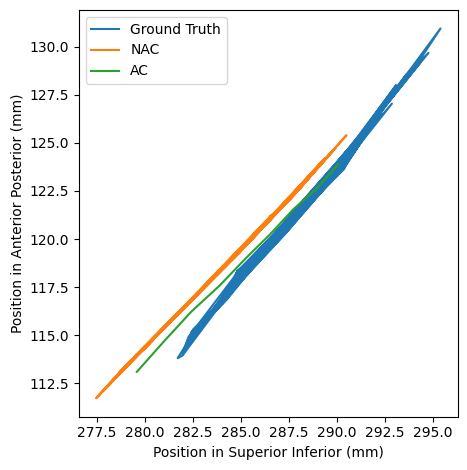
\includegraphics[width=1.0\linewidth]{figures/motion_correction_results_2_com.png}
                
                \captionsetup{singlelinecheck=false, justification=centering}
                \caption{The path of the \gls{COM} of the lesion, in voxel indices. Horizontal (respectively vertical) axis corresponds to motion in the \gls{SI} (respectively \gls{AP}). Different curves denote \gls{COM} displacement for  ground truth data, the estimated data from the \gls{NAC} based \gls{MM} and the estimated data from the \gls{AC} based \gls{MM}.}
                \label{fig:pet_ct_respiratory_motion_correction_with_a_single_attenuation_map_using_nac_derived_deformation_fields_results_com}
            \end{figure}
            
            \gls{COM} results can be seen in~\Fref{fig:pet_ct_respiratory_motion_correction_with_a_single_attenuation_map_using_nac_derived_deformation_fields_results_com}, the \gls{COM} of both the \gls{NAC} and \gls{AC} matches closely the ground truth \gls{COM}.
            
            \begin{figure}
                \centering
                
                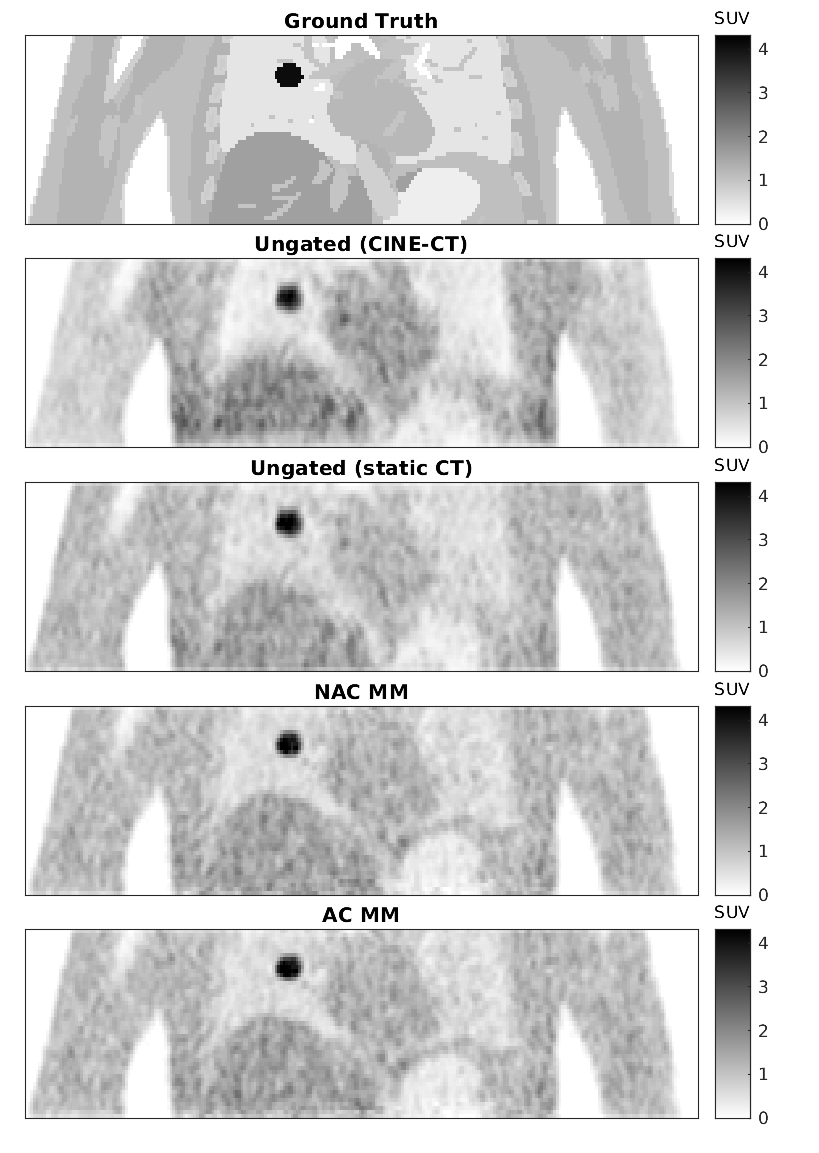
\includegraphics[width=1.0\linewidth]{figures/motion_correction_results_2_visual_analysis.png}
                
                \captionsetup{singlelinecheck=false, justification=centering}
                \caption{Ground truth and reconstructions using; ungated (CINE-\gls{CT}), ungated (static \gls{CT}), \gls{NAC} \gls{MM}, \gls{AC} \gls{MM}. Colour map ranges are consistent for all images.}
                \label{fig:pet_ct_respiratory_motion_correction_with_a_single_attenuation_map_using_nac_derived_deformation_fields_results_visual_analysis}
            \end{figure}
            
            \begin{figure}
                \centering
                
                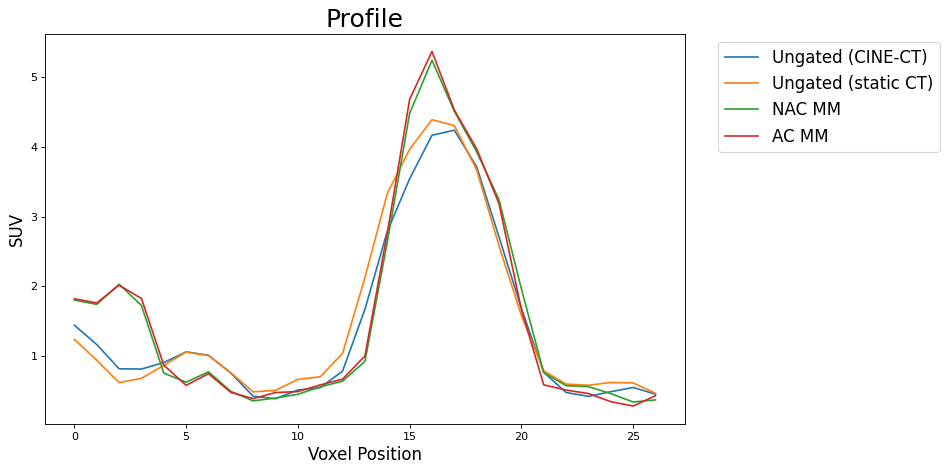
\includegraphics[width=1.0\linewidth]{figures/motion_correction_results_2_profile.png}
                
                \captionsetup{singlelinecheck=false, justification=centering}
                \caption{A profile across the lesion for; ungated (CINE-\gls{CT}), ungated (static \gls{CT}), \gls{NAC} \gls{MM}, \gls{AC} \gls{MM}.}
                \label{fig:pet_ct_respiratory_motion_correction_with_a_single_attenuation_map_using_nac_derived_deformation_fields_results_profile}
            \end{figure}
            
            \begin{table}
                \centering
                
                \captionsetup{singlelinecheck=false, justification=centering}
                \caption{Comparison of \gls{SUV}\textsubscript{max}, \gls{SUV}\textsubscript{median} and \gls{SUV}\textsubscript{peak} between; ungated (CINE-\gls{CT}), ungated (static \gls{CT}), \gls{NAC} \gls{MM}, \gls{AC} \gls{MM}.}
                
                \resizebox*{1.0\linewidth}{!}
                {
                    \begin{tabular}{||c|ccc||}
                        \hline
                        \textbf{\gls{SUV}} & \textbf{Max} & \textbf{Median} & \textbf{Peak} \\
                        \hline
                        \textbf{Ungated (CINE-\gls{CT})}    & $4.63$ & $2.73$ & $3.39$ \\
                        \textbf{Ungated (static \gls{CT})}  & $4.66$ & $3.05$ & $3.54$ \\
                        \hline
                        \textbf{\gls{NAC} \gls{MM}}         & $5.56$ & $3.18$ & $4.07$ \\
                        \textbf{\gls{AC} \gls{MM}}          & $5.43$ & $3.18$ & $4.00$ \\
                        \hline
                    \end{tabular}
                }
                \label{tab:pet_ct_respiratory_motion_correction_with_a_single_attenuation_map_using_nac_derived_deformation_fields_results_suv}
            \end{table}
            
             The ungated and the \gls{MM} data can be seen in~\Fref{fig:pet_ct_respiratory_motion_correction_with_a_single_attenuation_map_using_nac_derived_deformation_fields_results_visual_analysis}. When compared visually structures can be seen, less blurred, in the \gls{MM} data that cannot be seen in the ungated data, for instance, structures at the boundary between the diaphragm and the lung. The different levels of blurring in the ungated (CINE-\gls{CT}) and static \gls{CT} could be attributed to the constraint put on the reconstruction by having a sharp \gls{Mu-Map} in one respiratory position in the static \gls{CT} case. Additionally the lesion itself can be seen to be more homogeneous, this can be observed in the profile across the lesion in~\Fref{fig:pet_ct_respiratory_motion_correction_with_a_single_attenuation_map_using_nac_derived_deformation_fields_results_profile}. \gls{SUV} results can be seen in~\Fref{tab:pet_ct_respiratory_motion_correction_with_a_single_attenuation_map_using_nac_derived_deformation_fields_results_suv} and consistently show that \glss{SUV} are greater for the \gls{MM} over the ungated method.
            
        \subsection{Conclusion} \label{sec:pet_ct_respiratory_motion_correction_with_a_single_attenuation_map_using_nac_derived_deformation_fields_conclusion}
            Results from both a visual analysis, a comparison of profiles and \glss{SUV} show that the \gls{MM} provides volumes more free from blurring and less susceptible to artefacts when compared to the ungated data. Results also indicate that the \gls{NAC} \gls{MM} provides similar volumes while not requiring the additional computation of the \gls{AC} \gls{MM}. Results indicate that \gls{MC} of inter-respiratory cycle motion is possible with this method, while accounting for attenuation deformation.
            
            Future research includes the possibility of directly incorporating the \gls{MM} estimation or estimated \glss{DVF} into the reconstruction algorithm as well as  attempting to simultaneously estimate deformations for the \gls{Mu-Map} as well as the activity distribution. For instance, more complex methods of combining motion estimation and \gls{IR} based on~\boxcite{Bousse2016a}~\boxcite{Bousse2016} will also be compared. additionally it may also be possible to find better results from improvements to \gls{TOF} resolution~\boxcite{Efthimiou2020UseScanners, Efthimiou2020TOF-PETBGO}. This will be expanded upon in~\Fref{sec:impact_of_tof_on_respiratory_motion_model_estimation_using_nac_pet_discussion}.
    
    \longsection{Comparison of Motion Correction Methods Incorporating Motion Modelling for PET/CT Using a Single Breath Hold Attenuation Map}{sec:comparison_of_motion_correction_methods_incorporating_motion_modelling_for_pet/ct_using_a_single_breath_hold_attenuation_map}
        This section shows a comparison of different \gls{MC} techniques, including with and without incorporating \glss{MM}. The comparison shown here is presented on low count data, so as to better highlight the impact of the addition of \glss{MM}. The \glss{Mu-Map} used are at end inhalation to better reflect clinical breath hold \glss{Mu-Map}.
        
        \subsection{Introduction} \label{sec:comparison_of_motion_correction_methods_incorporating_motion_modelling_for_pet/ct_using_a_single_breath_hold_attenuation_map_introduction}
            \gls{MM} is a \gls{MC} technique, where time- or gate-dependence of \glss{DVF} is parametrised in terms of a \gls{SS}~\boxcite{McClelland2013}. \glss{MM} attempt to improve upon solely registering data, being more robust to noise, but also allowing for the correction of unseen data. It has shown good promise in \gls{CT}~\boxcite{Li2007EnhancedModel}, \gls{MR}~\boxcite{Manke2002RespiratoryModels} and combined \gls{PET}/\gls{MR}~\boxcite{Manber2016JointCorrection.}, but has not yet seen wide spread adoption in clinical \gls{PET}, where \gls{PET}/\gls{CT} is far more common. Respiratory \gls{MC} is an ideal problem area for the application of \glss{MM} as \glss{SS} are already commonly available from respiratory gating, such as acquired by \gls{RPM} or \gls{PCA}~\boxcite{Thielemans2011}.
            
            A method incorporating \glss{MM} for dynamic \gls{PET}/\gls{CT}, was proposed and tested on clinical data in~\boxcite{Chan2018Non-RigidPET}. This work seeks to extend the method, presented in~\Fref{sec:impact_of_tof_on_respiratory_motion_model_estimation_using_pre_gated_no_intra_cycle_motion_nac_pet} and~\Fref{sec:pet_ct_respiratory_motion_correction_with_a_single_attenuation_map_using_nac_derived_deformation_fields}, further through the use of a more modular framework, which allows for the fair comparison of different registration methods, both with and without \glss{MM}. Furthermore, this work uses more realistic simulation and count levels, compared to previous work (where more simple registration methods would fail). Additionally, this work strives to improve the \gls{Mu-Map} warping aspect of previous method, by fixing the \gls{Mu-Map} at end inhalation (as opposed to the mean respiratory position). This is more clinically relevant but also challenging. The work presented here, differentiates itself, specifically from previous work in \gls{MM} for \gls{PET}/\gls{CT}~\boxcite{Chan2018Non-RigidPET}, by firstly using a \gls{2D} \gls{SS}, rather than a \gls{1D} \gls{SS}, thus both inter- and intra-gate motion can be included in the model, at the expense that each gate contains fewer counts. Additionally, the group-wise method, presented here, makes use of an iterative \gls{MC} algorithm rather than using only a pair-wise method.
        
        \subsection{Methods} \label{sec:comparison_of_motion_correction_methods_incorporating_motion_modelling_for_pet/ct_using_a_single_breath_hold_attenuation_map_methods}
            \subsubsection{XCAT Volume Generation} \label{sec:comparison_of_motion_correction_methods_incorporating_motion_modelling_for_pet/ct_using_a_single_breath_hold_attenuation_map_xcat_volume_generation}
                Volume generation follows the same basic structure as presented in~\Fref{sec:impact_of_tof_on_respiratory_motion_model_estimation_using_pre_gated_no_intra_cycle_motion_nac_pet_methods_xcat_image_generation} and~\Fref{sec:impact_of_tof_on_respiratory_motion_model_estimation_using_pre_gated_no_intra_cycle_motion_nac_pet_methods_xcat_image_generation}. However the \gls{SS} used to drive \gls{XCAT} was derived from \gls{MR} navigator patient data and a \SI{20}{\milli\metre} diameter spherical lesion (smaller than the max displacement, due to \gls{RM}) was placed into the base of the right lung (within the max displacement, due to \gls{RM}, of the diaphragm).
            
            \subsubsection{PET Acquisition Simulation and Non-Attenuation Corrected Image Reconstruction} \label{sec:comparison_of_motion_correction_methods_incorporating_motion_modelling_for_pet/ct_using_a_single_breath_hold_attenuation_map_pet_acquisition_simulation_and_non_attenuation_corrected_image_reconstruction}
                Again as in~\Fref{sec:impact_of_tof_on_respiratory_motion_model_estimation_using_pre_gated_no_intra_cycle_motion_nac_pet_methods_pet_data_simulation} and~\Fref{sec:pet_ct_respiratory_motion_correction_with_a_single_attenuation_map_using_nac_derived_deformation_fields_methods_pet_acquisition_simulation} \gls{PET} acquisitions were simulated (and reconstructed) using \gls{STIR}~\boxcite{Thielemans2012}~\boxcite{Nikos2019} through \gls{SIRF}~\boxcite{Ovtchinnikov2017}. Attenuation was included using the relevant \glss{Mu-Map} generated by \gls{XCAT}. Pseudo-randoms and scatter were added. Randoms were added by summing the scaled mean value to each voxel of each volume prior to forward projection. Pseudo scatter was added by summing the scaled and smoothed mean \gls{Mu-Map} prior to forward projection, the smoothing parameter was optimised to give scatter which tapered at the same rate as in clinical data A full scatter simulation was not performed due to software limitations.
                
                Noise was simulated, such that data matched an acquisition over \SI{120}{\second}, emulating a standard single bed position acquisition. The count rate was selected to match that of research scans, i.e. below that of diagnostic clinical scans. This count rate was selected as a 'worst case scenario'.
                
                A respiratory \gls{SS} was generated using \gls{PCA}~\boxcite{Thielemans2011}. The magnitude of this signal and its gradient, was used to gate data into $30$ respiratory bins using displacement gating ($10$ amplitude and $3$ gradient bins). Gates with fewer than $0.42$\% of the counts were discarded. For the purpose of the \gls{MM} fitting, \gls{SS} values were determined for the post-gated data by taking an average of the \gls{SS} values of data in each bin.
                
                Data were reconstructed, without \gls{AC}, using \gls{OSEM} with two full iterations and $24$ subsets~\boxcite{Hudson1994}.
            
            \subsubsection{Registration} \label{sec:comparison_of_motion_correction_methods_incorporating_motion_modelling_for_pet/ct_using_a_single_breath_hold_attenuation_map_registration}
                Before being registered, each volume underwent pre-processing. Including, replication of end-slices, transformation to be approximately normally distributed~\boxcite{Johnson2013} and post-smoothing. This pre-processing was only applied to intermediate data and was not used for the final output of the method.% Initially, because a breath hold \gls{Mu-Map} is the final target position for the \gls{MC} $10$ repeating slices are added to the top and bottom of each volume to allow space for the volumes to be registered into. First, the mean value was subtracted from each volume and then each voxel in the volume was divided by the standard deviation of the volume. Next a Yeo-Johnson transformation~\boxcite{Johnson2013} was applied to transform data to be more Gaussian like, this acted as a pseudo histogram normalisation. Finally data underwent Gaussian smoothing.
                
                Two registration methods were examined in this work. Firstly, pair-wise registration, where the reference position was selected as the gate with the highest number of counts. All other gates were registered to it. Secondly, group-wise registration, where after an initial pair-wise registration step, the \glss{DVF} generated had the inverse mean of all \glss{DVF} composed with them, before a new reference volume was resampled. Registration to the new reference volume, followed by the inverse mean composition and resample, continued for a set number of iterations. NiftyReg~\boxcite{Modat2010} was used to perform registrations using a B-spline parameterisation. The Gaussian smoothing \gls{FWHM}, \gls{CPG} spacing of the B-spline coefficients, \gls{BE} regularisation term weight and number of iterations were tuned using a grid search.
            
            \subsubsection{Motion Model Estimation} \label{sec:comparison_of_motion_correction_methods_incorporating_motion_modelling_for_pet/ct_using_a_single_breath_hold_attenuation_map_motion_model_estimation}
                If a \gls{MM} was used, then it was fit as a direct \gls{RCM} on the \glss{DVF} from~\Fref{sec:comparison_of_motion_correction_methods_incorporating_motion_modelling_for_pet/ct_using_a_single_breath_hold_attenuation_map_registration} and the \gls{SS} from~\Fref{sec:comparison_of_motion_correction_methods_incorporating_motion_modelling_for_pet/ct_using_a_single_breath_hold_attenuation_map_pet_acquisition_simulation_and_non_attenuation_corrected_image_reconstruction}. A weighted \gls{LR} was used, where the weighting was taken based on the number of counts in each gate. Once a \gls{MM} was fit, new \glss{DVF} were generated for each gate, using the \gls{SS} values used to fit the \gls{MM}. For group-wise registration, \gls{MM} fitting occurred between iterations, the \glss{DVF} generated by the \gls{MM} were used to resample the new target volume at each iteration.
            
            \subsubsection{Attenuation Map Warping} \label{sec:comparison_of_motion_correction_methods_incorporating_motion_modelling_for_pet/ct_using_a_single_breath_hold_attenuation_map_attenuation_map_warping}
                A \gls{Mu-Map} at end inhalation was selected from the \glss{Mu-Map} generated by \gls{XCAT}. The \gls{PET} volume from the previous step was then registered to this \gls{Mu-Map}, and the resulting \glss{DVF} were composed with the \glss{DVF} from the last iteration of the \gls{MC} method, and a new volume resampled. The inverse of these \glss{DVF}, were then used to warp the \gls{Mu-Map} to each gate.
            
            \subsubsection{Motion Corrected Image Reconstruction with AC} \label{sec:comparison_of_motion_correction_methods_incorporating_motion_modelling_for_pet/ct_using_a_single_breath_hold_attenuation_map_attenuation_corrected_image_reconstruction}
                Data were re-reconstructed with \gls{AC}, using the \glss{Mu-Map} from~\Fref{sec:comparison_of_motion_correction_methods_incorporating_motion_modelling_for_pet/ct_using_a_single_breath_hold_attenuation_map_attenuation_map_warping}. The same reconstruction parameters as in~\Fref{sec:comparison_of_motion_correction_methods_incorporating_motion_modelling_for_pet/ct_using_a_single_breath_hold_attenuation_map_attenuation_corrected_image_reconstruction} were used. \gls{MC} was then applied to data following~\Fref{sec:comparison_of_motion_correction_methods_incorporating_motion_modelling_for_pet/ct_using_a_single_breath_hold_attenuation_map_registration},~\Fref{sec:comparison_of_motion_correction_methods_incorporating_motion_modelling_for_pet/ct_using_a_single_breath_hold_attenuation_map_motion_model_estimation} and~\Fref{sec:comparison_of_motion_correction_methods_incorporating_motion_modelling_for_pet/ct_using_a_single_breath_hold_attenuation_map_attenuation_map_warping}. Volumes were post-filtered using a Gaussian smoothing, with a \gls{FWHM} of \SI{6.39}{\milli\metre} in the transverse plane (equivalent to three voxels) and \SI{3.27}{\milli\metre} (equivalent to one voxel) in the axial direction.
            
            \subsubsection{Evaluation} \label{sec:comparison_of_motion_correction_methods_incorporating_motion_modelling_for_pet/ct_using_a_single_breath_hold_attenuation_map_evaluation}
                In addition to the reconstructions performed in~\Fref{sec:comparison_of_motion_correction_methods_incorporating_motion_modelling_for_pet/ct_using_a_single_breath_hold_attenuation_map_attenuation_corrected_image_reconstruction}, data were also reconstructed without \gls{MC}, using either a sum of all \glss{Mu-Map} (to emulate an \gls{AV-CCT}), or the end inhalation \gls{Mu-Map}. For the present evaluation, the volumes without \gls{MC} were registered to the position of the end inhalation \gls{Mu-Map}. Additionally, \glss{DVF} generated by each method were also applied to noiseless data for visual analysis.
                
                Comparisons used included: A profile over the lesion, \gls{SUV}\textsubscript{max} and \gls{SUV}\textsubscript{peak} (defined following \gls{EANM} guidelines~\boxcite{Boellaard2015FDG2.0}).
        
        \subsection{Results} \label{sec:comparison_of_motion_correction_methods_incorporating_motion_modelling_for_pet/ct_using_a_single_breath_hold_attenuation_map_results}
            \begin{figure}
                \centering
                
                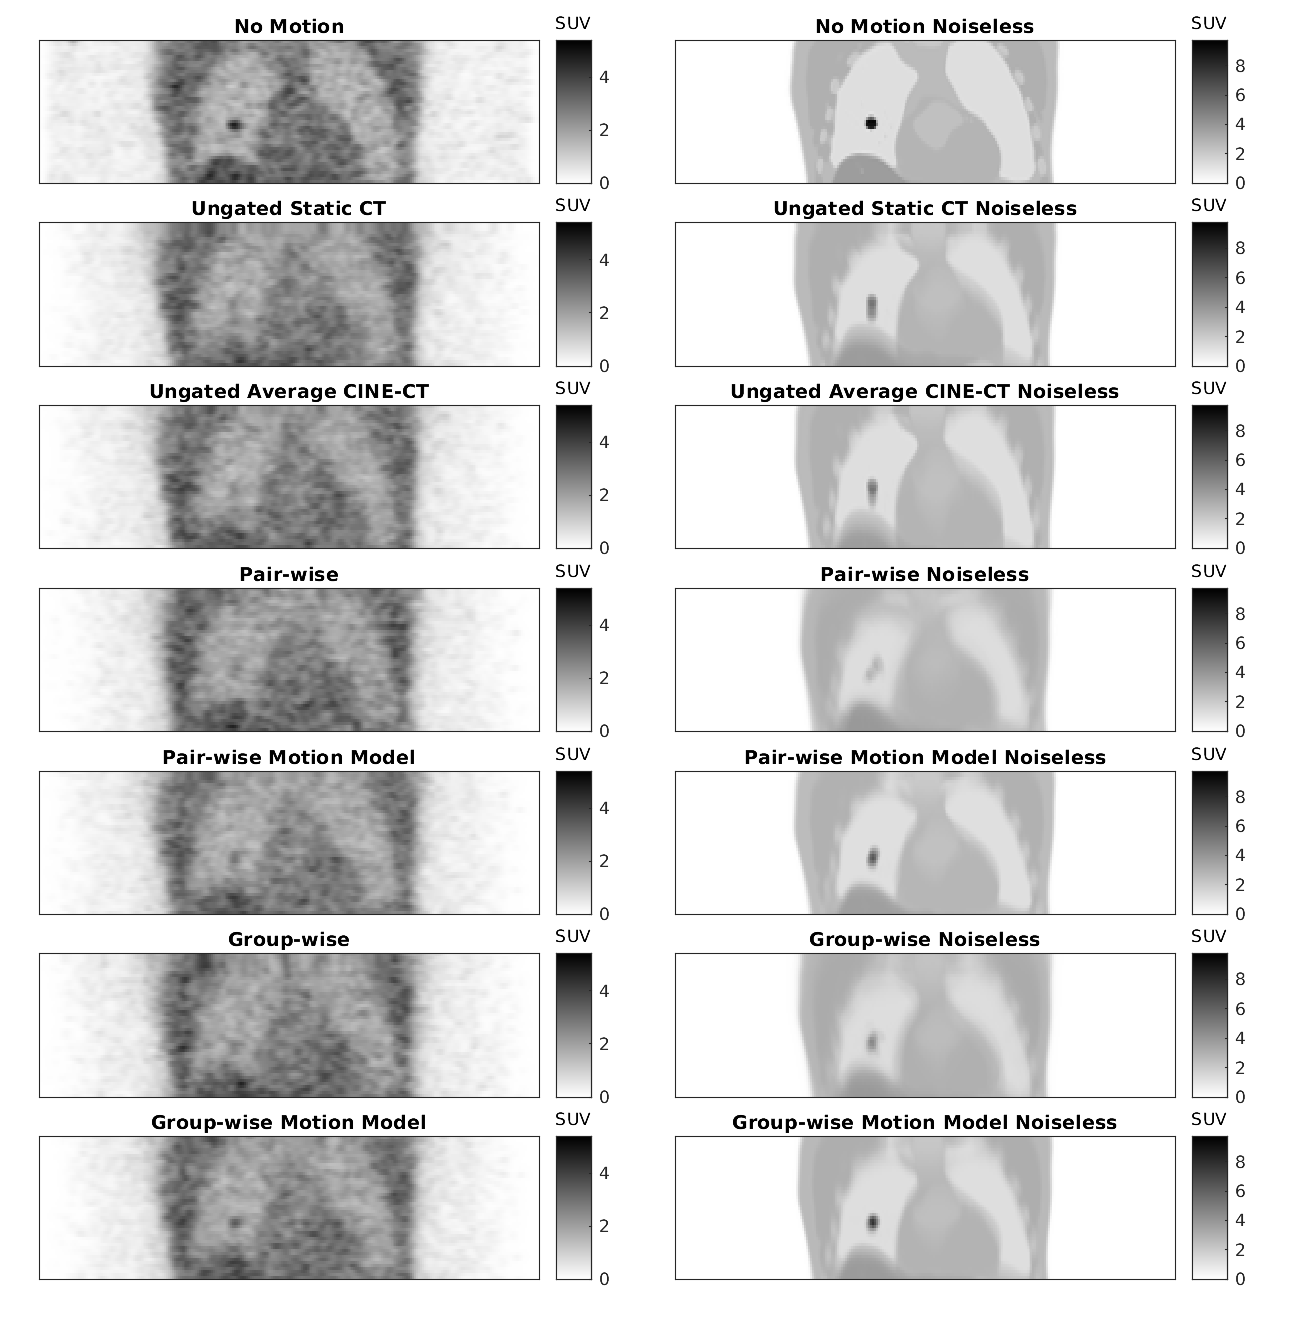
\includegraphics[width=1.0\linewidth]{figures/motion_correction_results_3_visual_analysis.png}
                
                \captionsetup{singlelinecheck=false, justification=centering}
                \caption{First column contains \gls{AC} \gls{MC} reconstructions and the second column contains the result of applying the final  \gls{MC} on the original XCAT images (for easier assessment of the accuracy of the estimated \glss{DVF}); ungated static \gls{CT}, ungated \gls{AV-CCT}, pair-wise, pair-wise \gls{MM}, group-wise, group-wise \gls{MM}. Colour map ranges are consistent for all images in each column.}
                \label{fig:comparison_of_motion_correction_methods_incorporating_motion_modelling_for_pet/ct_using_a_single_breath_hold_attenuation_map_visual_analysis}
            \end{figure}
            
            \begin{figure}
                \centering
                
                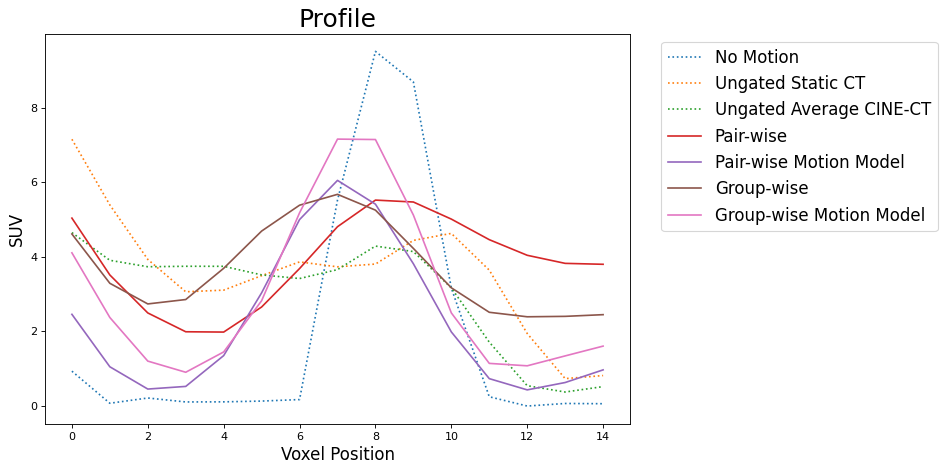
\includegraphics[width=1.0\linewidth]{figures/motion_correction_results_3_profile.png}
                
                \captionsetup{singlelinecheck=false, justification=centering}
                \caption{A profile across the lesion for; ungated static \gls{CT}, ungated \gls{AV-CCT}, pair-wise, pair-wise \gls{MM}, group-wise, group-wise \gls{MM}.}
                \label{fig:comparison_of_motion_correction_methods_incorporating_motion_modelling_for_pet/ct_using_a_single_breath_hold_attenuation_map_profile}
            \end{figure}
            
            \begin{table}
                \centering
                
                \captionsetup{singlelinecheck=false, justification=centering}
                \caption{Comparison of \gls{SUV}\textsubscript{max} and \gls{SUV}\textsubscript{peak} between: ungated static \gls{CT}, ungated \gls{AV-CCT}, pair-wise, pair-wise \gls{MM}, group-wise, group-wise \gls{MM}.}
                
                \resizebox*{1.0\linewidth}{!}
                {
                    \begin{tabular}{||c|cc||}
                        \hline
                        \textbf{\gls{SUV}}                  & \textbf{Max}  & \textbf{Peak} \\
                        \hline
                        \textbf{No Motion}                  & $9.50$        & $9.06$ \\
                        \hline
                        \textbf{Ungated Static \gls{CT}}    & $5.25$        & $5.15$ \\
                        \textbf{Ungated \gls{AV-CCT}}       & $5.38$        & $5.07$ \\
                        \hline
                        \textbf{Pair-wise}                  & $4.21$        & $3.92$ \\
                        \textbf{Pair-wise \gls{MM}}         & $6.63$        & $6.07$ \\
                        \hline
                        \textbf{Group-wise}                 & $4.42$        & $4.21$ \\
                        \textbf{Group-wise \gls{MM}}        & $7.64$        & $7.03$ \\
                        \hline
                    \end{tabular}
                }
                \label{tab:comparison_of_motion_correction_methods_incorporating_motion_modelling_for_pet/ct_using_a_single_breath_hold_attenuation_map_suv}
            \end{table}
            
            A visual comparison of the reconstructed images (see ~\Fref{fig:comparison_of_motion_correction_methods_incorporating_motion_modelling_for_pet/ct_using_a_single_breath_hold_attenuation_map_visual_analysis}), shows that more blurring can be seen at the boundary between the diaphragm and lung for the \gls{MM}-free methods. Additionally, where a \gls{MM} was used, the lesion appears to be more homogeneous.
             
            The peak of the profile (see~\Fref{fig:comparison_of_motion_correction_methods_incorporating_motion_modelling_for_pet/ct_using_a_single_breath_hold_attenuation_map_profile}), is greater for \gls{MM} methods than for \gls{MM}-free methods. However, the peak for all \gls{MC} methods are greater than ungated methods.
             
            \gls{SUV} results consistently show that including \glss{MM} increases the \gls{SUV} when compared to when one is not used (see~\Fref{tab:comparison_of_motion_correction_methods_incorporating_motion_modelling_for_pet/ct_using_a_single_breath_hold_attenuation_map_suv}).
        
        \subsection{Conclusion} \label{sec:comparison_of_motion_correction_methods_incorporating_motion_modelling_for_pet/ct_using_a_single_breath_hold_attenuation_map_conclusions}
            Results from a visual analysis, a comparison of profiles and \gls{SUV}, show that adding a \gls{MM} to any \gls{MC} method (tested here) improved the quality of volumes produced. Although, from a visual analysis volumes appear preferable with any \gls{MC} method, quantitative evaluation points to the conclusion that for \gls{MC} to be successful, for very noisy data, \glss{MM} are almost required.
            
            In the future, work will focus on incorporating the methods presented here into an iterative \gls{PET} reconstruction and \gls{MC} method and tested on patient data from several research studies. It may also be of interest to consider the impact that robust regression methods have on fitting a \gls{MM}, such as using a robust objective function or fitting the \gls{MM} indirectly on the eigenvectors of applying \gls{PCA} to the initial \glss{DVF}.
    
    \longsection{Discussion}{sec:impact_of_tof_on_respiratory_motion_model_estimation_using_nac_pet_discussion}
        The methods presented above suffer from a number of issues which future work will seek to rectify. Firstly, an obvious hole in the results presented above is that the method has only been tested on simulated data. Thus, it cannot be said that if the method works here that it can be extrapolated that it also works on clinical data. For instance, the initial activity distributions are taken from \gls{XCAT} simulated volumes, these volumes suffer from the fact that within a feature they are almost entirely homogeneous. If the intensity of the activity volume were examined the intensity within an organ or tissue would almost never vary. This actually poses a significant problem to most registration algorithms, where there would be no gradient across a homogeneous region thus the reconstruction is more likely to terminate early with a poor result or otherwise be unable to find a good direction to update in.
        
        An additional issue posed by the use of \gls{XCAT} simulations would be that the \gls{MM} used to drive the simulation over time is rather simple, it is a linear \gls{MM}. This means that for a given value of the \gls{SS} the anatomy will always be in the same place. Whereas, a patient is more likely to have breath to breath variability and the motion present will almost never be able to be entirely represented by a linear system. The \gls{MM} method used in the work above also uses a linear \gls{MM}, meaning that all of the motion present in the data could be captured unadulterated by the method (under ideal circumstances) possibly giving misleading results. The fact that the \gls{MM} used is linear in and of itself could be a limitation, a patient is unlikely to breath following a linear model. As such when it is possible to test the method using data generated using a non-linear model, it could be advantageous to also incorporate a non-linear model into the \gls{MM}.
        
        Furthermore, the \gls{SS} used during the \gls{XCAT} simulation, for most of this work, is identical (but flipped) for both the \gls{AP} and \gls{SI} motion. This means that there is no hysteresis in the motion, which is unrealistic. This could be solved by giving separate signals (a \gls{2D} signal) for both the \gls{AP} and \gls{SI} motion, which are captured using an \gls{MR} scanner, rather than a \gls{1D} signal captured from an \gls{RPM}. This has begun to be addressed by using an \gls{MR} derived signal in~\Fref{sec:comparison_of_motion_correction_methods_incorporating_motion_modelling_for_pet/ct_using_a_single_breath_hold_attenuation_map}.
        
        The anatomy used for the \gls{XCAT} simulation did not vary, it was an average male anatomy. In order to prove generalisability, and to avoid unnecessary bias, ideally the method would be tested on a multitude of anatomy including both male and female, big and small. This is compounded by the fact that the lesion used to demonstrate the improvement by the \gls{MC} method was unreasonably large, \gls{MC} wouldn't be needed to identify and locate it. In order to better highlight the advantage of the \gls{MC} method a smaller lesion placed closer to the diaphragm should be used. This also has begun to be addressed in~\Fref{sec:comparison_of_motion_correction_methods_incorporating_motion_modelling_for_pet/ct_using_a_single_breath_hold_attenuation_map}.
        
        Although \gls{18F-FDG} is the most commonly used radiotracer, it isn't the only used radiotracer. If this method were used during cardiac imaging it most likely wouldn't be the radiotracer used. Given this, the activity values used during the \gls{XCAT} simulation were taken from a clinical \gls{18F-FDG} scan and as such the method hasn't been tested in these circumstances.
        
        The method to simulate the \gls{PET} acquisition also has some limitations. Firstly, in the work presented here a relatively high count rate is used for the noise caused by the \gls{PET} acquisition physics. It may be interesting to look at how the \gls{MC} methods perform under more strenuous circumstance, for instance, research scan count rate levels. Additionally, as mentioned above in both~\Fref{sec:impact_of_tof_on_respiratory_motion_model_estimation_using_pre_gated_no_intra_cycle_motion_nac_pet_methods_pet_data_simulation} and~\Fref{sec:pet_ct_respiratory_motion_correction_with_a_single_attenuation_map_using_nac_derived_deformation_fields_methods_pet_acquisition_simulation} no random or scatter simulation were used. This is clearly unrealistic as a \gls{PET} scan could never take place without either random or scatter events, even if they were corrected for. The reason for a lack of random or scatter simulation was because the software available did not provide this functionality when using \gls{TOF} simulations. This has begun to be addressed in~\Fref{sec:comparison_of_motion_correction_methods_incorporating_motion_modelling_for_pet/ct_using_a_single_breath_hold_attenuation_map}. This is being addressed using a lower count simulation and also by including pseudo-random and scatter.
        
        \gls{TOF} resolutions used in the work are not reflected in any current scanner. The \gls{TOF} resolution in conjunction with the voxel size were chosen as a compromise between two current systems to give the method the best chance of working. However, obviously this means there is no clinical data available to test the method on that wouldn't also mean changing one of either the \gls{TOF} resolution or the voxel size. If the \gls{GE} Discovery $710$ were selected to perform scans to test this method it would also mean sacrificing some \gls{TOF} resolution.
        
        Building from the limitations highlighted in the \gls{MC} and \gls{MM} earlier, the registrations performed as part of the \gls{MM} were fit using \gls{SSD}. This objective function is sensitive to differences in the magnitude of the input. If gates are registered to a mean volume, as in group-wise registration seen earlier in~\Fref{sec:applying_image_registration}, then the magnitude of the inputs will never be equal. Additionally, if \gls{SSD} were used to register a \gls{PET} activity distribution to a \gls{CT} \gls{Mu-Map} it would also fail for the same reasons. This problem could be solved by preprocessing the data, however, it could also be addressed by changing the objective function to something such as \gls{NMI}. This has begun to be addressed in~\Fref{sec:comparison_of_motion_correction_methods_incorporating_motion_modelling_for_pet/ct_using_a_single_breath_hold_attenuation_map}. Here \gls{NMI} was included, however this the method used did not fit the \gls{MC} and \gls{MM} simultaneously.
        
        Furthermore, the objective function used for the \gls{MM} fitting also used \gls{SSD} which is sensitive to outliers. This would cause a limitation during early iterations of the \gls{MC} when it is likely that the quality of the registration is poor and thus the B-spline coefficients or the \gls{DVF} is also poor. This limitation may be compounded if the method were combined, as is, iteratively with \gls{PET} reconstruction. This is because, at early time points not only would the registration be poor but the volumes provided to the registration by the reconstruction would also be poor. To mitigate this an objective function which is robust to outliers could be used, such as Huber. Huber is defined as being equivalent to squared error below a threshold and absolute error above it.
        
        A final limitation and a possible future direction for research would be that the objective function for the registration is currently calculated in image space. If the objective function were shifted to sinogram space then it would be much more likely that a combined iterative \gls{PET} reconstruction and \gls{MC} would converge to a good solution due to the fact that both methods are using objective functions calculated in the same space.

    \chapter{Data Driven Surrogate Signal Extraction for Dynamic PET} \label{sec:data_driven_surrogate_signal_extraction_results}
    \newpage
    
    \longsection{Introduction}{sec:data_driven_surrogate_signal_extraction_results_introduction}
        This chapter of the thesis contains work performed in the domain of \gls{SS} extraction from dynamic \gls{PET} data. The first section of this chapter introduces preliminary work performed using the \gls{PCA} method, including ventures to improve its robustness to variation caused by radiotracer kinetics.
    
    \longsection{PCA Data Driven Surrogate Signal Extraction Methods for Dynamic PET}{sec:pca_data_driven_surrogate_signal_extraction_methods_for_Dynamic_pet}
        This section investigates \gls{DD} methods to extract \gls{SS} from dynamic \gls{PET}, in particular this section will discuss methods using \gls{PCA} and compare them to similar methods, from the literature, some of which use \gls{SAM}.
        
        \subsection{Introduction} \label{sec:pca_data_driven_surrogate_signal_extraction_methods_for_dynamic_pet_introduction}
            As discussed in~\Fref{sec:respiratory_motion_in_pet} and \Fref{sec:impact_of_tof_on_respiratory_motion_model_estimation_using_nac_pet} respiratory motion correction is beneficial in positron emission tomography. Respiratory motion reduces image resolution in \gls{PET} by introducing blurring and mis-alignment artefacts~\boxcite{Nehmeh2008a}. Methods of motion correction include gated reconstruction, where the acquisition is binned based on a respiratory trace. Gating requires a \gls{SS} which reflects the position the patient is in the respiratory cycle over time. Methods to determine \glss{SS} include those which use an external device, like the \gls{RPM}. However, a disadvantage of these methods is that they require the use of additional equipment and a change to clinical practise. Thus, \gls{DD} methods to extract \glss{SS} have become an alternative, for more detail see~\Fref{sec:data_driven}. 
            
            However, data driven methods have the disadvantage that they are adversely affected by the radiotracer kinetics of a dynamic acquisition. Current \gls{DD} \gls{SS} extraction methods struggle with dynamic \gls{PET} data where the radiotracer kinetics, at the start of the acquisition, offer more variance than the respiratory motion does. In~\Fref{sec:data_driven}, the application of \gls{PCA} for data-driven respiratory surrogate signal extraction was described. As \gls{PCA} orders the eigenvectors according to the magnitude of the variance of their contribution to the data. In static thoracic \gls{PET}, the first few components will usually contain information on the \gls{RM} of the patient, but this might not be the case for dynamic \gls{PET}. Previously, work was performed to extend the \gls{SAM} method to be robust to radiotracer kinetics, this work proposed the use of \gls{STFT} to generate masks for the \gls{SAM} method (rather than a static mask for all time points), this was called \gls{KRG}~\boxcite{Schleyer2014}. \gls{STFT} operates by splitting the data into windows and doing a \gls{FFT} on them independently, this could be approximated by windowing the data first and then performing \gls{SAM}. This section seeks to evaluate several adaptions of the \gls{PCA} method through which it can be used with dynamic data. The methods explored in this section include the use of a moving window, and also re-use of the \glss{PC} from a later time point to estimate the \gls{SS} from earlier time points.
        
        \subsection{Methods} \label{sec:pca_data_driven_surrogate_signal_extraction_methods_for_dynamic_pet_methods}
            \begin{figure}
                \centering
                
                \includegraphics[width=0.3\linewidth]{figures/data_driven_surrogate_signal_extraction_methods_1_overview.png}
                
                \captionsetup{singlelinecheck=false, justification=centering}
                \caption{A diagram showing an overview of the possible ways in which the method could be executed.}
                \label{fig:pca_data_driven_surrogate_signal_extraction_methods_for_dynamic_pet_methods_overview}
            \end{figure}
            
            The following subsections will address the method with respect to the diagram seen in~\Fref{fig:pca_data_driven_surrogate_signal_extraction_methods_for_dynamic_pet_methods_overview}. Additionally, a full combined diagram can be seen in~\Fref{sec:pca_data_driven_surrogate_signal_extraction_methods_for_dynamic_pet_full_overview} in~\Fref{fig:pca_data_driven_surrogate_signal_extraction_methods_for_dynamic_pet_appendix_full_overview}.
            
            \subsection{Data Acquisition} \label{sec:pca_data_driven_surrogate_signal_extraction_methods_for_dynamic_pet_methods_data_acquisition}
                Data was used from a research study with patients suffering from idiopathic pulmonary fibrosis. $21$ dynamic \gls{18F-FDG} acquisitions, with a \gls{FOV} covering the upper lung and heart, were acquired on a \gls{GE} Discovery $710$. Each acquisition lasted approximately \SI{20}{\minute} with the acquisition starting before injection of the radiotracer. \glss{SS} were acquired in parallel using a \gls{RPM}.
                
            \subsection{Data Preparation} \label{sec:pca_data_driven_surrogate_signal_extraction_methods_for_dynamic_pet_methods_data_preparation}
                \begin{figure}
                    \centering
                    
                    \includegraphics[width=0.4\linewidth]{figures/data_driven_surrogate_signal_extraction_methods_1_pre_processing.png}
                    
                    \captionsetup{singlelinecheck=false, justification=centering}
                    \caption{A diagram showing pre-processing performed.}
                    \label{fig:pca_data_driven_surrogate_signal_extraction_methods_for_dynamic_pet_methods_pre_processing}
                \end{figure}
                
                Data were unlisted into low spatial resolution sinograms, each with time frame duration of \SI{500}{\milli\second}, using the \gls{GE} PetToolbox following~\boxcite{Bertolli2018Data-DrivenTomography} resulting in sinograms with dimensions $95 x 16 x 47 x 11$ (radial positions $x$ angles $x$ transaxial plane $x$ \gls{TOF}). Data was pre-processed by first applying a Freeman-Tukey transformation~\boxcite{Freeman1950TransformationsRoot} before then applying a Yeo-Johnson power transformation~\boxcite{Yeo2000ASymmetry}, this is in order to attempt to transform the Poisson distributed data to be more Gaussian-like. The Freeman-Tukey transformation was applied before the Yeo-Johnson power transformation as it was found that the Freeman-Tukey transformation made the Yeo-Johnson power transformation more reliable. Furthermore, it was also found that adding the Yeo-Johnson power transformation gave better results than the Freeman-Tukey transformation alone.
                
                The Freeman-Tukey transformation is defined as:

                \begin{equation} \label{eq:pca_data_driven_surrogate_signal_extraction_methods_for_dynamic_pet_methods_freeman_tukey}
                    S_g := \sqrt{S_p + 1} + \sqrt{S_p}
                \end{equation}

                \noindent where in~\Fref{eq:pca_data_driven_surrogate_signal_extraction_methods_for_dynamic_pet_methods_freeman_tukey} $S_g$ is the resultant, approximately Gaussian distributed, sinogram and $S_p$ is the original Poisson distributed sinogram $S_p$~\boxcite{Freeman1950TransformationsRoot}.
                
                The Yeo-Johnson power transformation is defined as:

                \begin{equation} \label{eq:pca_data_driven_surrogate_signal_extraction_methods_for_dynamic_pet_methods_yeo_johnson}
                    S_g := \begin{cases}
                                ((S_p + 1)^\lambda - 1) / \lambda                   & \quad \text{if } \lambda \neq 0 \text{, } S_p \geq 0 \\
                                \log(S_p + 1)                                       & \quad \text{if } \lambda = 0 \text{, } S_p \geq 0    \\
                                -[(-S_p + 1)^{(2 - \lambda)} - 1)] / (2 - \lambda)  & \quad \text{if } \lambda \neq 2 \text{, } S_p < 0    \\
                                -\log(-S_p + 1)                                     & \quad \text{if } \lambda = 2 \text{, } S_p < 0
                            \end{cases}
                \end{equation}

                \noindent where in~\Fref{eq:pca_data_driven_surrogate_signal_extraction_methods_for_dynamic_pet_methods_yeo_johnson} $S_g$ is the resultant, approximately Gaussian distributed, sinogram. The $\lambda$ parameter is determined by minimising the Kullback-Leibler distance between normal distributions and the transformed distribution~\boxcite{Yeo2000ASymmetry}. In the current implementation, a single $\lambda$ is determined from all of the data, although it would be feasible to find different $\lambda$ values for every element in the sinogram.
                    
                It has been found through experimentation that Gaussian smoothing can improve results, especially in the case of the \gls{SAM} methods. Further downsampling can be performed post-smoothing to reduce memory usage, in this case linear interpolation has been found to be satisfactory and additionally is less computationally expensive to calculate than some methods, however Akima spline interpolation has been shown to give marginally improved results but is significantly more computationally expensive~\boxcite{Akima1970AProcedures}.
                        
                Additionally, it has been found that the introduction of a mask to aid in the reduction of noise is beneficial \boxcite{Thielemans2011}. Both types of method can be used with a mask. The mask itself is defined as being true for any value in the sinogram above a predetermined threshold, values not in the mask are removed prior to further execution. Note that a mask can also be used to eliminate parts of the data potentially affected by non-respiratory movement~\boxcite{Bertolli2018Data-DrivenTomography}, but this has not been implemented in the current method yet.
                
                A flowchart of the above can be seen in~\Fref{fig:pca_data_driven_surrogate_signal_extraction_methods_for_dynamic_pet_methods_pre_processing}.
            
            \subsection{Surrogate Signal Extraction} \label{sec:pca_data_driven_surrogate_signal_extraction_methods_for_dynamic_pet_methods_surrogate_signal_extraction}
                \begin{figure}
                    \centering
                    
                    \includegraphics[width=0.7\linewidth]{figures/data_driven_surrogate_signal_extraction_methods_1_get_signal.png}
                    
                    \captionsetup{singlelinecheck=false, justification=centering}
                    \caption{A diagram showing the methods to get a signal.}
                    \label{fig:pca_data_driven_surrogate_signal_extraction_methods_for_dynamic_pet_methods_get_signal}
                \end{figure}
                
                \subsubsection{Applying PCA} \label{sec:pca_data_driven_surrogate_signal_extraction_methods_for_dynamic_pet_methods_applying_pca}
                    Again, as can be seen from the diagram in~\Fref{fig:pca_data_driven_surrogate_signal_extraction_methods_for_dynamic_pet_methods_overview} there are three methods of applying \gls{PCA} (these methods could also be used with \gls{SAM} but for simplicity we will refer specifically to \gls{PCA} here).
                    
                    \begin{itemize}
                        \item Firstly there is what shall be referred to as the static method. Here, \gls{PCA} is applied to the entire data set in one go as it would be if the data were from a static acquisition, hence the name.
                        
                        \item Secondly there is the moving window method. Here the data is split into a series of windows, where each subsequent window overlaps with the previous window by half its length. The size of each window is predetermined and selected experimentally. The motivation for attempting the moving window method is to increase the relative importance of motion vs kinetics, this is achieved through small windows being used at early time points, where the radiotracer kinetics are at their most severe, and longer windows can be used at later time points to reduce noise.
                        
                        For this method \gls{PCA} is applied independently on each window and the results are averaged together after sign correction. The windows overlap as the sign of the signal from each window is arbitrary and the overlapping allows for a common sign to be found by comparing the \gls{CC} of neighbouring windows and flipping windows where the \gls{CC} is negative. If \gls{SAM} is used rather than \gls{PCA} here then the method approximates \gls{KRG}~\boxcite{Schleyer2014}.

                        \item Finally there is the one \gls{PC} method where \glss{PC} from late time points are taken and used with early time point data. The motivation for attempting this method is that it was observed that \glss{PC} for late time point data didn't vary significantly when different windows were selected, however that was not true for early time point data. It could be hypothesised that because the \gls{RM} should be semi-consistent throughout the acquisition, then if a \gls{PC} is capturing the \gls{RM} at late time points then it should do the same at early time points.
                        
                        The one \gls{PC} method splits the data into two channels, one which only contains later time point data where the radiotracer kinetics have diminished and one which contains all the data. The cutoff between early and later time point data is determined experimentally. \gls{PCA} is applied to the later time point data only. The \glss{PC} from the later time point data can then be taken and multiplied by the channel containing all of the data to give the weights contributing to that \gls{PC} for all time points.
                        
                        The generic equation for calculating the weights (or signal) from the \gls{PC} and data is defined as:

                        \begin{equation} \label{eq:pca_data_driven_surrogate_signal_extraction_methods_for_dynamic_pet_methods_pc_weights}
                            W := PC \cdot D
                        \end{equation}
        
                        \noindent where in~\Fref{eq:pca_data_driven_surrogate_signal_extraction_methods_for_dynamic_pet_methods_pc_weights} $W$ is the weights (or signal) found when multiplying the \gls{PC} $PC$ by data $D$ and summing. In fact, a similar equation is used by \gls{SAM}, where a "signed mask" is multiplied with the data and summed. Therefore this method would be applicable to SAM as well, although this has not been done yet in this work.
                    \end{itemize}
                    
                    A flowchart of the above can be seen in~\Fref{fig:pca_data_driven_surrogate_signal_extraction_methods_for_dynamic_pet_methods_get_signal}.
                
                \subsubsection{Selecting and Combining PCs} \label{sec:pca_data_driven_surrogate_signal_extraction_methods_for_dynamic_pet_methods_selecting_and_combining_pcs}
                    \begin{figure}
                        \centering
                        
                        \includegraphics[width=0.7\linewidth]{figures/data_driven_surrogate_signal_extraction_methods_1_select_and_combine.png}
                        
                        \captionsetup{singlelinecheck=false, justification=centering}
                        \caption{A diagram showing how \glss{PC} can be selected and combined.}
                        \label{fig:pca_data_driven_surrogate_signal_extraction_methods_for_dynamic_pet_methods_select_and_combine}
                    \end{figure}
                
                    \begin{algorithm}
                        \caption{Get respiratory kinetic ratio and respiratory noise ratio}
                        \KwData{\glss{PC}}
                        \KwResult{respiratory kinetic ratio and respiratory noise ratio}
                        \;
                        $PSD$ := \gls{FFT} on current \gls{PC}\;
                        \;
                        $kineticContribution$ := mean of $PSD$ between \SI{0.0}{\hertz} and \SI{0.1}{\hertz}\;
                        $respiratoryContribution$ := mean of $PSD$ between \SI{0.1}{\hertz} and \SI{0.4}{\hertz}\;
                        $noiseContribution$ := mean of $PSD$ above \SI{0.4}{\hertz}\;
                        \;
                        $respiratoryKineticRatio$ := $respiratoryContribution$ / $kineticContribution$\;
                        $respiratoryNoiseRatio$ := $respiratoryContribution$ / $noiseContribution$\;
                        \;
                    \end{algorithm} \label{eq:pca_data_driven_surrogate_signal_extraction_methods_for_dynamic_pet_methods_selecting_and_combining_pcs_get respiratory_kinetic_ratio_and_respiratory_noise_ratio_pseudo_code}
                    
                    \begin{algorithm}
                        \caption{Selecting \glss{PC}}
                        \KwData{\glss{PC}}
                        \KwResult{selected \glss{PC}}
                        \;
                        \For{\gls{PC} in $PCs$}{
                            $RKRatio$, $RNRatio$ := get respiratory kinetic ratio and respiratory noise ratio from current \gls{PC}\;
                            \;
                            $RKRatioList$ append $RKRatio$\;
                            $RNRatioList$ append $RNRatio$\;
                        }
                        \;
                        remove \gls{PC} from $PCs$ where $RKRatioList$ \textless 1\;
                        remove \gls{PC} from $PCs$ where $RNRatioList$ \textless 1\;
                        \;
                        $PCs$ := $PCs$ * ($RKRatioList$ * $RNRatioList$)\;
                        order $PCs$\;
                    \end{algorithm} \label{eq:pca_data_driven_surrogate_signal_extraction_methods_for_dynamic_pet_methods_selecting_pcs_pseudo_code}
                    
                    \begin{algorithm}
                        \caption{Combining \glss{PC}}
                        \KwData{selected \glss{PC}}
                        \KwResult{respiratory \gls{PC}}
                        \;
                        $respiratoryPC$ := first \gls{PC} in $PCs$\;
                        remove $respiratoryPC$ from $PCs$\;
                        $RKRatio$, $RNRatio$ := get respiratory kinetic ratio and respiratory noise ratio from $respiratoryPC$\;
                        \;
                        \For{\gls{PC} in $PCs$}{
                            $sumPC$ := $respiratoryPC$ + current \gls{PC}\;
                            $subtractPC$ := $respiratoryPC$ - current \gls{PC}\;
                            \;
                            $sumRKRatio$, $sumRNRatio$ := get respiratory kinetic ratio and respiratory noise ratio from $sumPC$\;
                            $subtractRKRatio$, $subtractRNRatio$ := get respiratory kinetic ratio and respiratory noise ratio from $subtractPC$\;
                            \;
                            \eIf{$sumRKRatio$ \textgreater $RKRatio$}{
                                \uIf{$sumRNRatio$ \textgreater $RNRatio$}{
                                    $respiratoryPC$ := $sumPC$\;
                                    $RKRatio$ := $sumRKRatio$\;
                                    $RNRatio$ := $sumRNRatio$\;
                                }
                            }{
                                \uIf{$subtractRKRatio$ \textgreater $RKRatio$}{
                                    \uIf{$subtractRNRatio$ \textgreater $RNRatio$}{
                                        $respiratoryPC$ := $subtractPC$\;
                                        $RKRatio$ := $subtractRKRatio$\;
                                        $RNRatio$ := $subtractRNRatio$\;
                                    }
                                }
                            }
                        }
                    \end{algorithm} \label{eq:pca_data_driven_surrogate_signal_extraction_methods_for_dynamic_pet_methods_combining_pcs_pseudo_code}
                    
                    Furthermore, as an additional development of the previous methods a way to combine \glss{PC} was proposed. The motivation for this was that it could be observed that signals in the frequency window of \gls{RM} could be seen outside of the first few \glss{PC}. Additionally, a significant number of these had far less of a frequency contribution in the frequency window of the radiotracer kinetics. However, they may not be selected if only one \gls{PC} is used and determined by the greatest mean frequency contribution in the respiratory window, as in~\boxcite{Thielemans2011}, and~\boxcite{Bertolli2018Data-DrivenTomography}. This could lead to a reduced \gls{SNR}.
                    
                    Firstly, pseudo code of the above method can be seen in~\Fref{eq:pca_data_driven_surrogate_signal_extraction_methods_for_dynamic_pet_methods_selecting_and_combining_pcs_get respiratory_kinetic_ratio_and_respiratory_noise_ratio_pseudo_code}, ~\Fref{eq:pca_data_driven_surrogate_signal_extraction_methods_for_dynamic_pet_methods_selecting_pcs_pseudo_code} and~\Fref{eq:pca_data_driven_surrogate_signal_extraction_methods_for_dynamic_pet_methods_combining_pcs_pseudo_code}. A flowchart of the above can be seen in~\Fref{fig:pca_data_driven_surrogate_signal_extraction_methods_for_dynamic_pet_methods_select_and_combine}.
                    
                    In order to exploit those \glss{PC}, first the \gls{PSD} of each signal must be calculated using \gls{FFT}. These \gls{PSD} contain the frequency contribution of each signal between the frequencies of \SI{0.0}{\hertz} and \SI{1.0}{\hertz} (due to the frame duration). Next, frequency windows representing the content of information related to radiotracer kinetics, \gls{RM} and noise are defined. In the current implementation they are defined as \SI{0.0}{\hertz} to \SI{0.1}{\hertz}, \SI{0.1}{\hertz} to \SI{0.4}{\hertz} and above \SI{0.4}{\hertz} respectively. The contribution within each window is determined for each \gls{PC} by finding the mean magnitude within the windows. Ratios are then determined between the respiratory window and the kinetic window and the respiratory window and the noise window. Data are ordered such that the respiratory to kinetic window ratio is maximised, in other words the \gls{PC} which contributes the most respiratory information without contributing much kinetic information goes first. Any \gls{PC} where more noise is contributed than useful respiratory information, defined as a threshold on the noise to respiratory ratio, is then thrown away.
                    
                    In the order determined in the previous step the \glss{PC} are looped over and both summed and subtracted with a weighting (the respiratory to kinetic ratio multiplied by the respiratory to noise ratio for each \gls{PC}) and a new \gls{PSD} is found for both resulting signals. If one of the signals increases the respiratory frequency contribution more than the kinetic or noise contribution then it becomes the new best \gls{PC} and goes forward to the next iteration. \glss{PC} are both summed and subtracted to deal with the arbitrary sign problem mentioned earlier~\Fref{sec:pca_data_driven_surrogate_signal_extraction_methods_for_dynamic_pet_methods_applying_pca}. A similar method of combining signals can be seen in~\boxcite{Kesner2010AMethods}. However, the method presented here has the advantage over the method presented in~\boxcite{Kesner2010AMethods} as the metric to define a good signal here specifically looks to maximise a value related to the behaviour desired. However, in~\boxcite{Kesner2010AMethods} the standard deviation is maximised which could logically be increased through means other than those desired. In addition, the proposed method applies the metric on \glspl{PC} as opposed to single voxel or sinogram bin values, which should lead to noise reduction.
                
                \subsubsection{Post-Processing} \label{sec:pca_data_driven_surrogate_signal_extraction_methods_for_dynamic_pet_methods_post_processing}
                    \begin{figure}
                        \centering
                        
                        \includegraphics[width=0.3\linewidth]{figures/data_driven_surrogate_signal_extraction_methods_1_parallel_compression.png}
                        
                        \captionsetup{singlelinecheck=false, justification=centering}
                        \caption{A diagram showing the parallel compression method.}
                        \label{fig:pca_data_driven_surrogate_signal_extraction_methods_for_dynamic_pet_methods_parallel_compression}
                    \end{figure}
                    
                    \begin{figure}
                        \centering
                        
                        \includegraphics[width=0.5\linewidth]{figures/data_driven_surrogate_signal_extraction_methods_1_post_processing.png}
                        
                        \captionsetup{singlelinecheck=false, justification=centering}
                        \caption{A diagram showing the post-processing performed.}
                        \label{fig:pca_data_driven_surrogate_signal_extraction_methods_for_dynamic_pet_methods_post_processing}
                    \end{figure}
                    
                    A flowchart of the method can be seen in~\Fref{fig:pca_data_driven_surrogate_signal_extraction_methods_for_dynamic_pet_methods_parallel_compression} and~\Fref{fig:pca_data_driven_surrogate_signal_extraction_methods_for_dynamic_pet_methods_post_processing}.
                    
                    Regardless of method used there are still some effects of the radiotracer kinetics to be expected at early time points and noise throughout. Thus a method of parallel compression has been proposed here to deal with the remaining radiotracer kinetics and a plethora of smoothing to deal with the noise.
                    
                    \begin{itemize}
                        \item Firstly there is, what shall be referred to as, parallel compression. This is a method borrowed from audio engineering (appearing notably in Dolby A noise reduction) whereby the signal is split into two channels, one has its dynamic range decimated while the other passes unchanged before they are summed back together~\boxcite{Izhaki2012MixingTools}. This has the effect of reducing large differences in the dynamic range of the signal without losing a lot of breath to breath variability. In order to achieve this here the signal is split into two channels and one channel is further split into a series of small moving windows. The channel comprised of windows now has the median value of each window subtracted and each window divided by its \gls{MAD}. This channel then has its windows averaged back together before being combined with the unadulterated channel. The channels are combined following the gradient of the head count signal, the absolute value of the signal is first taken before it is normalised between zero and one, where it is larger more of the compressed signal is summed. The head count signal is the sum of the sinogram at each time point.
                        
                        \item Even though most of the large macro changes in intensity are dealt with by parallel compression some momentary spikes still make it through the process. Thus outliers are removed where they are outside a threshold of the quantile of the signal and new values are interpolated.
                        
                        \item Smoothing is applied first through the use of a bandpass filter before a Savitzky-Golay filter is applied. A Savitzky-Golay filter is a moving window polynomial filter~\boxcite{Savitzky1964SmoothingProcedures}. The parameters of both are determined through experimentation.
                    \end{itemize}
            
            \subsection{Evaluation} \label{sec:pca_data_driven_surrogate_signal_extraction_methods_for_dynamic_pet_methods_evaluation}
                Parameters for the methods have been selected through a grid search using a subset of the data available, specifically three patients. The parameters were optimised by maximising the \gls{CC} between the \gls{SS} and the \gls{RPM} for the first \SI{60}{\second} of the acquisition. For evaluation of the results the \gls{CC} of each \gls{SS} between each method and the \gls{RPM}, for all acquisitions, has been calculated. The \gls{CC} has been calculated for both the first \SI{60}{\second} and also the entire acquisition. This is because, if the method works then it is expect the radiotracer redistribution will have the most impact in the first \SI{60}{\second} of the acquisition.
            
        \subsection{Results} \label{sec:pca_data_driven_surrogate_signal_extraction_methods_for_dynamic_pet_results}
            \begin{figure}
                \centering
                
                \includegraphics[width=1.0\linewidth]{figures/data_driven_surrogate_signal_extraction_results_1_vanilla_surrogate_signal.png}
                
                \captionsetup{singlelinecheck=false, justification=centering}
                \caption{A visual comparison between the \gls{RPM} \gls{SS} and the \gls{SS} from the static \gls{PCA} method using only the first \gls{PC} for three patients between \SI{20}{\second} and \SI{160}{\second}. The three patients shown here are the ones on which parameters for the method were optimised.}
                \label{fig:pca_data_driven_surrogate_signal_extraction_methods_for_dynamic_pet_results_vanilla_surrogate_signal}
            \end{figure}
            
            \begin{figure}
                \centering
                
                \includegraphics[width=1.0\linewidth]{figures/data_driven_surrogate_signal_extraction_results_1_combined_surrogate_signal.png}
                
                \captionsetup{singlelinecheck=false, justification=centering}
                \caption{A visual comparison between the \gls{RPM} \gls{SS} and the \gls{SS} from the static \gls{PCA} method by combining the first $20$ \glss{PC} for three patients between \SI{20}{\second} and \SI{160}{\second}. The three patients shown here are the ones on which parameters for the method were optimised. Here no pre- or post-processing is used.}
                \label{fig:pca_data_driven_surrogate_signal_extraction_methods_for_dynamic_pet_results_combined_surrogate_signal}
            \end{figure}
            
            \begin{figure}
                \centering
                
                \includegraphics[width=1.0\linewidth]{figures/data_driven_surrogate_signal_extraction_results_1_box_plot.png}
                
                \captionsetup{singlelinecheck=false, justification=centering}
                \caption{A box plot of the \gls{CC} between static \gls{PCA} method both when using only the first \gls{PC} and by combining the first $20$ \glss{PC} for all patients between \SI{20}{\second} and \SI{160}{\second} and for the entire acquisition. The parameters used here were optimised for and frozen based on the results shown in other diagrams on three patients. Here no pre- or post-processing is used.}
                \label{fig:pca_data_driven_surrogate_signal_extraction_methods_for_dynamic_pet_results_box_plot}
            \end{figure}
            
            \begin{figure}
                \centering
                
                \includegraphics[width=1.0\linewidth]{figures/data_driven_surrogate_signal_extraction_results_1_combined_surrogate_signal_processed.png}
                
                \captionsetup{singlelinecheck=false, justification=centering}
                \caption{A visual comparison between the \gls{RPM} \gls{SS} and the \gls{SS} from the static \gls{PCA} method by combining the first $20$ \glss{PC} for three patients between \SI{20}{\second} and \SI{160}{\second}. The three patients shown here are the ones on which parameters for the method were optimised. Here pre- and post-processing are used.}
                \label{fig:pca_data_driven_surrogate_signal_extraction_methods_for_dynamic_pet_results_combined_surrogate_signal_processed}
            \end{figure}
            
            \begin{figure}
                \centering
                
                \includegraphics[width=1.0\linewidth]{figures/data_driven_surrogate_signal_extraction_results_1_box_plot_processed.png}
                
                \captionsetup{singlelinecheck=false, justification=centering}
                \caption{A box plot of the \gls{CC} between static \gls{PCA} method both when using only the first \gls{PC} and by combining the first $20$ \glss{PC} for all patients between \SI{20}{\second} and \SI{160}{\second} and for the entire acquisition. The parameters used here were optimised for and frozen based on the results shown in other diagrams on three patients. Here pre- and post-processing are used.}
                \label{fig:pca_data_driven_surrogate_signal_extraction_methods_for_dynamic_pet_results_box_plot_processed}
            \end{figure}
            
            Results presented here are only for the static \gls{PCA} case, results for other methods are in preparation. For results presented here parameters were selected on a subset of the data (specifically three randomly selected scans) before being applied across the entire data set. A plot of the \gls{SS} for static \gls{PCA} using only one \gls{PC} for three patients at early time points can be seen in~\Fref{fig:pca_data_driven_surrogate_signal_extraction_methods_for_dynamic_pet_results_vanilla_surrogate_signal}. It can be observed in this example that only using the static \gls{PCA} method and one \gls{PC} does not give satisfactory results at early time points. A plot of the \gls{SS} for static \gls{PCA} using a combination of the first $20$ \glss{PC} for three patients at early time points can be seen in~\Fref{fig:pca_data_driven_surrogate_signal_extraction_methods_for_dynamic_pet_results_combined_surrogate_signal}, here no pre- or post-processing is used. Here for all patients from very early in the acquisition it can be seen that the method gives comparable results to the \gls{RPM}. A plot of the \gls{SS} for static \gls{PCA} using a combination of the first $20$ \glss{PC} for three patients at early time points can be seen in~\Fref{fig:pca_data_driven_surrogate_signal_extraction_methods_for_dynamic_pet_results_combined_surrogate_signal_processed}, here pre- and post-processing are used. The parameters for the processing were optimised solely to improve the \gls{CC} for early time points, as such it can be seen that some inter-window variation has been removed (from parallel compression).
            
            A box plot of the \gls{CC} of the \gls{SS} for static \gls{PCA} using only one \gls{PC} compared to the \gls{RPM} and the \gls{CC} of the \gls{SS} for static \gls{PCA} using a combination of the first $20$ \glss{PC} compared to the \gls{RPM} for all patients at both early time points and all time points and  can be seen in~\Fref{fig:pca_data_driven_surrogate_signal_extraction_methods_for_dynamic_pet_results_box_plot}, here no pre- or post-processing is used. Here the improvement by incorporating multiple \glss{PC} is most apparent. A box plot of the \gls{CC} of the \gls{SS} for static \gls{PCA} using only one \gls{PC} compared to the \gls{RPM} and the \gls{CC} of the \gls{SS} for static \gls{PCA} using a combination of the first $20$ \glss{PC} compared to the \gls{RPM} for all patients at both early time points and all time points and  can be seen in~\Fref{fig:pca_data_driven_surrogate_signal_extraction_methods_for_dynamic_pet_results_box_plot_processed}, here pre- and post-processing are used. The parameters for the processing were optimised solely to improve the \gls{CC} for early time points, as such it can be seen that the \gls{CC} drops from no processing to processing for the entire acquisition, it can be assumed this effect is similar to minimising variance at the expense of bias or vice versa.
            
        \subsection{Discussion and Conclusion} \label{sec:pca_data_driven_surrogate_signal_extraction_methods_for_dynamic_pet_discussion_and_conclusion}
            Results from a visual comparison of early time point signals from both an \gls{RPM} and static \gls{PCA} indicates that without combining \glss{PC} results for early time points are poor, however the method of combining \glss{PC} presented here has good promise, this is further reinforced when the \gls{CC} is examined.
            
            In the future, research will focus on further development of the method, tuning the parameters of the additional methods to the point where they can be compared. In the next stage, the methods will be evaluated when used in combination with respiratory motion correction techniques.
            
            The work presented here suffers from a few limitations. Firstly the data taken here all comes from the same study, using the same procedure, the same radiotracer and acquired on the same scanner. In order to better validate the generalisability of the method it would be positive to test on data acquired on different scanners and using different radiotracers.
            
            An additional concern is that the method could fail for patients who exhibit abnormal breathing patters. For instance, extremely slow breathers will breathe at a rate less than \SI{0.1}{\hertz}, which here would be considered to be radiotracer kinetics. Furthermore, the method struggles with patients who breathe at less regular intervals, exemplified by those who occasionally hold their breath or otherwise stop breathing for periods and by those who breathe in such a way as to induce multiple harmonics in their breathing, this could be seen as a signal atop a carrier. One method which could be developed to combat these issues would be to introduce machine learning, either to completely replace the method or to enhance it. A \gls{NN} could be added here to replace the three window method of selecting and combining \glss{PC}, a \gls{NN} could be trained to identify signals which are caused by respiration. There are already \glss{NN} which are designed to discriminate between data, such as the aptly named discriminator \gls{NN} used as part of training a \gls{GAN}.
    
%    \longsection{Feasibility Study of Neural Network Based Data Driven Surrogate Signal Extraction Methods for Dynamic PET}{sec:feasibility_study_of_neural_network_based_data_driven_surrogate_signal_extraction_methods_for_dynamic_pet}
        
        
%        \subsection{Introduction} \label{sec:feasibility_study_of_neural_network_based_data_driven_surrogate_signal_extraction_methods_for_dynamic_pet_introduction}
            
        
%        \subsection{Methods} \label{sec:feasibility_study_of_neural_network_based_data_driven_surrogate_signal_extraction_methods_for_dynamic_pet_methods}
            
            
%        \subsection{Results} \label{sec:feasibility_study_of_neural_network_based_data_driven_surrogate_signal_extraction_methods_for_dynamic_pet_results}
            
            
%        \subsection{Discussion and Conclusion} \label{sec:feasibility_study_of_neural_network_based_data_driven_surrogate_signal_extraction_methods_for_dynamic_pet_discussion_and_conclusion}

    \chapter{Discussion and Conclusion} \label{sec:discussion_and_conclusion}
    \newpage
    
    \longsection{Introduction}{sec:discussion_and_conclusion_introduction}
        This chapter will recap the discussion from previous chapters before 

    \addcontentsline{toc}{chapter}{Appendices}

\chapter{Appendices}
    \newpage
    % The \appendix command resets the chapter counter, and changes the chapter numbering scheme to capital letters.
    \appendix
    
    \chapter{PCA Data Driven Surrogate Signal Extraction Methods for Dynamic PET Full Overview} \label{sec:pca_data_driven_surrogate_signal_extraction_methods_for_dynamic_pet_full_overview}
    \newpage

    \begin{figure}
        \centering
        
        \includegraphics[width=0.2\linewidth]{figures/data_driven_surrogate_signal_extraction_methods_1_full_overview.png}
        
        \captionsetup{singlelinecheck=false, justification=centering}
        \caption{A diagram showing an overview of the possible ways in which the method could be executed.}
        \label{fig:pca_data_driven_surrogate_signal_extraction_methods_for_dynamic_pet_appendix_full_overview}
    \end{figure}

    \chapter{PCA Data Driven Surrogate Signal Extraction Methods for Dynamic PET Results With and Without Pre- and Post-Processing} \label{sec:pca_data_driven_surrogate_signal_extraction_methods_for_dynamic_pet_results_with_and_without_pre_and_post_processing_appendix}
    \newpage

    \begin{figure}
        \centering
        
        \includegraphics[width=1.0\linewidth]{figures/data_driven_surrogate_signal_extraction_results_1_vanilla_surrogate_signal.png}
        
        \captionsetup{singlelinecheck=false}
        \caption{
            A visual comparison between the \gls{RPM} \gls{SS} and the \gls{SS} from the static \gls{PCA} method using only the first \gls{PC} for three patients between \SI{20}{\second} and \SI{160}{\second}. The three patients shown here are the ones on which parameters for the method were optimised.
        }
        \label{fig:pca_data_driven_surrogate_signal_extraction_methods_for_dynamic_pet_results_with_and_without_pre_and_post_processing_appendix_vanilla_surrogate_signal}
    \end{figure}
    
    \begin{figure}
        \centering
        
        \includegraphics[width=1.0\linewidth]{figures/data_driven_surrogate_signal_extraction_results_1_combined_surrogate_signal.png}
        
        \captionsetup{singlelinecheck=false}
        \caption{
            A visual comparison between the \gls{RPM} \gls{SS} and the \gls{SS} from the static \gls{PCA} method by combining the first $20$ \glspl{PC} for three patients between \SI{20}{\second} and \SI{160}{\second}. The three patients shown here are the ones on which parameters for the method were optimised. Here no pre- or post-processing is used.
        }
        \label{fig:pca_data_driven_surrogate_signal_extraction_methods_for_dynamic_pet_results_with_and_without_pre_and_post_processing_appendix_combined_surrogate_signal}
    \end{figure}
    
    \begin{figure}
        \centering
        
        \includegraphics[width=1.0\linewidth]{figures/data_driven_surrogate_signal_extraction_results_1_box_plot.png}
        
        \captionsetup{singlelinecheck=false}
        \caption{
            A box plot of the \gls{CC} between static \gls{PCA} method both when using only the first \gls{PC} and by combining the first $20$ \glspl{PC} for all patients between \SI{20}{\second} and \SI{160}{\second} and for the entire acquisition. The parameters used here were optimised for and frozen based on the results shown in other diagrams on three patients. Here no pre- or post-processing is used.
        }
        \label{fig:pca_data_driven_surrogate_signal_extraction_methods_for_dynamic_pet_results_with_and_without_pre_and_post_processing_appendix_box_plot}
    \end{figure}
    
    \begin{figure}
        \centering
        
        \includegraphics[width=1.0\linewidth]{figures/data_driven_surrogate_signal_extraction_results_1_combined_surrogate_signal_processed.png}
        
        \captionsetup{singlelinecheck=false}
        \caption{
            A visual comparison between the \gls{RPM} \gls{SS} and the \gls{SS} from the static \gls{PCA} method by combining the first $20$ \glspl{PC} for three patients between \SI{20}{\second} and \SI{160}{\second}. The three patients shown here are the ones on which parameters for the method were optimised. Here pre- and post-processing are used.
        }
        \label{fig:pca_data_driven_surrogate_signal_extraction_methods_for_dynamic_pet_results_with_and_without_pre_and_post_processing_appendix_combined_surrogate_signal_processed}
    \end{figure}
    
    \begin{figure}
        \centering
        
        \includegraphics[width=1.0\linewidth]{figures/data_driven_surrogate_signal_extraction_results_1_box_plot_processed.png}
        
        \captionsetup{singlelinecheck=false}
        \caption{
            A box plot of the \gls{CC} between static \gls{PCA} method both when using only the first \gls{PC} and by combining the first $20$ \glspl{PC} for all patients between \SI{20}{\second} and \SI{160}{\second} and for the entire acquisition. The parameters used here were optimised for and frozen based on the results shown in other diagrams on three patients. Here pre- and post-processing are used.
        }
        \label{fig:pca_data_driven_surrogate_signal_extraction_methods_for_dynamic_pet_results_with_and_without_pre_and_post_processing_appendix_box_plot_processed}
    \end{figure}
    
    Results presented here are only for the static \gls{PCA} case. For results presented here parameters were selected on a subset of the data (specifically three randomly selected scans) before being applied across the entire data set. A plot of the \gls{SS} for static \gls{PCA} using only one \gls{PC} for three patients at early time points can be seen in~\Fref{fig:pca_data_driven_surrogate_signal_extraction_methods_for_dynamic_pet_results_with_and_without_pre_and_post_processing_appendix_vanilla_surrogate_signal}. It can be observed in this example that only using the static \gls{PCA} method and one \gls{PC} does not give satisfactory results at early time points. A plot of the \gls{SS} for static \gls{PCA} using a combination of the first $20$ \glspl{PC} for three patients at early time points can be seen in~\Fref{fig:pca_data_driven_surrogate_signal_extraction_methods_for_dynamic_pet_results_with_and_without_pre_and_post_processing_appendix_combined_surrogate_signal}, here no pre- or post-processing is used. Here for all patients from very early in the acquisition it can be seen that the method gives comparable results to the \gls{RPM}. A plot of the \gls{SS} for static \gls{PCA} using a combination of the first $20$ \glspl{PC} for three patients at early time points can be seen in~\Fref{fig:pca_data_driven_surrogate_signal_extraction_methods_for_dynamic_pet_results_with_and_without_pre_and_post_processing_appendix_combined_surrogate_signal_processed}, here pre- and post-processing are used. The parameters for the processing were optimised solely to improve the \gls{CC} for early time points, as such it can be seen that some inter-window variation has been removed (from parallel compression).
    
    A box plot of the \gls{CC} of the \gls{SS} for static \gls{PCA} using only one \gls{PC} compared to the \gls{RPM} and the \gls{CC} of the \gls{SS} for static \gls{PCA} using a combination of the first $20$ \glspl{PC} compared to the \gls{RPM} for all patients at both early time points and all time points and  can be seen in~\Fref{fig:pca_data_driven_surrogate_signal_extraction_methods_for_dynamic_pet_results_with_and_without_pre_and_post_processing_appendix_box_plot}, here no pre- or post-processing is used. Here the improvement by incorporating multiple \glspl{PC} is most apparent. A box plot of the \gls{CC} of the \gls{SS} for static \gls{PCA} using only one \gls{PC} compared to the \gls{RPM} and the \gls{CC} of the \gls{SS} for static \gls{PCA} using a combination of the first $20$ \glspl{PC} compared to the \gls{RPM} for all patients at both early time points and all time points and  can be seen in~\Fref{fig:pca_data_driven_surrogate_signal_extraction_methods_for_dynamic_pet_results_with_and_without_pre_and_post_processing_appendix_box_plot_processed}, here pre- and post-processing are used. The parameters for the processing were optimised solely to improve the \gls{CC} for early time points, as such it can be seen that the \gls{CC} drops from no processing to processing for the entire acquisition, it can be assumed this effect is similar to minimising variance at the expense of bias or vice versa.

    \chapter{Pseudo-Bayesian DIP Denoising as a Preprocessing Step for Kinetic Modelling in Dynamic PET} \label{sec:pseudo_bayesian_dip_denoising_as_a_preprocessing_step_for_kinetic_modelling_in_dynamic_pet}
    \newpage

    \section{Abstract} \label{sec:pseudo_bayesian_dip_denoising_as_a_preprocessing_step_for_kinetic_modelling_in_dynamic_pet_appendix_abstract}
        Noise (among other artefacts) could be considered to be the bane of \gls{PET}. %Often, it causes what could otherwise be a more simple problem to explode in complexity. 
        Many methods have been proposed to alleviate the worst annoyances of noise, however, not many take into account the temporal nature of dynamically acquired \gls{PET}. Here, we propose an adaption of a method, which has seen increasing attention in more traditional imaging denoising circles. \gls{DIP} exploits the initialisation of a carefully designed \gls{NN}, so as to treat it as a bank of custom filters, which are to be trained and used afresh on each new image, independently. \gls{DIP} has seen adaptation to \gls{PET} previously (including dynamic \gls{PET}), however, many of these adaptations do not take into account the large memory requirements of the method. Additionally, most previous work does not address the main weakness of the \gls{DIP}, its stopping criteria. Here, we propose a method which is both memory efficient, and includes a smoothing regularisation. In addition, we provide uncertainty estimates by incorporating a Bayesian approximation (using dropout), and prototype a training scheme by which the model is fit on all data simultaneously. The denoised images are then used as input for kinetic modelling. To evaluate the method, dynamic \gls{XCAT} simulations have been produced, with a \gls{FOV} of the lung and liver. The results of the new methods (along with \gls{TV} and the old \gls{DIP}) have been compared by; a visual analysis, \gls{SSIM}, and $K_i$ values. Results indicate that the new methods potentially outperform the old methods, without increasing computation time, while reducing system requirements.

    \section{Introduction} \label{sec:pseudo_bayesian_dip_denoising_as_a_preprocessing_step_for_kinetic_modelling_in_dynamic_pet_appendix_introduction}
        Most \gls{MLe} or \gls{NN} based methods, rely upon a workflow where a model is designed, trained, validated, and deployed~\parencite{Krose1993AnNetworks}. %This is logical as the intention with \gls{NN} based methods is to treat them as a general function approximator~\parencite{Krose1993AnNetworks}. This is where the function is determined by the relationship between the data used and the objective or loss function. 
        However, in the domain of image denoising, the \gls{DIP} method has received attention as training and inference are performed independently on each new image~\parencite{Ulyanov2020DeepPrior}.% The \gls{DIP} method could be considered to be a custom learnt bank of filters for each input. In order to prevent overfitting, the number of iterations used is imperative.% The authors of the original \gls{DIP} paper argue that the method could be considered to be used to solve many inverse problems~\parencite{Ulyanov2020DeepPrior}.
        
        For \gls{PET}, there have been a number of adaptations of \gls{DIP}.~\parencite{Gong2019PETPrior} used a U-Net with relatively high count/low motion brain scans~\parencite{Weng2021INet:Segmentation}. In~\parencite{Hashimoto20214DNetwork} \gls{DIP} is extended to \gls{4D} dynamic \gls{PET}. To do this, multiple output branches are grafted onto the \gls{NN}, one for each dynamic time point.~\parencite{Hashimoto2019DynamicDatasets} uses the original or static \gls{PET} acquisition as input to the \gls{NN}, rather than noise.~\parencite{Yang2022SimultaneousPrior} represents a more recent extension, where multiple \glss{NN} are used simultaneously.
        
        This work seeks to extend or simplify previous work, in order to denoise \gls{4D} dynamic \gls{PET} data.
    \section{Methods}\label{sec:pseudo_bayesian_dip_denoising_as_a_preprocessing_step_for_kinetic_modelling_in_dynamic_pet_appendix_methods}
        \subsection{Network Design and Execution} \label{sec:pseudo_bayesian_dip_denoising_as_a_preprocessing_step_for_kinetic_modelling_in_dynamic_pet_appendix_methods_network_design_and_execution}
            Firstly, we reduced \gls{GPU} memory requirements. Because \gls{DIP} requires training at inference, the full amount of memory is needed every time the method is used. To aid in clinical adoption, a hard limit of \SI{8.0}{\giga\byte} \gls{GPU} memory was imposed. Secondly, a more robust stopping criteria is required.% The stopping criteria should be flexible so as to allow the method to correct a wider variety of inputs. 
            % One method would be, to look at a window of previous loss function values, and exit, when the gradient of this drops below a tolerance.
            To aid in achieving this, as well as to address weaknesses of the original \gls{DIP}, regularisation must be added, so as to stop the \gls{NN} fitting to noise, similar to~\parencite{Liu2019ImagePrior}. Finally, because the output from this method is to be used in a further kinetic model fitting, it may provide improved results to have a metric of the uncertainty in the denoised images. we used dropout as in~\parencite{Gal2016DropoutLearning} to approximate (more expensive) Bayesian inference. Furthermore, this work uses \gls{PET} data with a \gls{FOV} of the lung and liver, whereas most previous work uses a \gls{FOV} of the head.
        
            The \gls{NN} used was a modified U-Net~\parencite{Weng2021INet:Segmentation}, with seven down/upsampling stages. Each down/upsampling stage consisted of two convolutional layers (with two, four, eight, $16$, $32$, $64$, or $128$ channels, depending on depth). Followed by, either a split strided convolution and maxpooling layer (with the result concatenated), or a trilinear upsampling layer. Edge padding, group normalisation~\parencite{Wu2020GroupNormalization}, MISH activation~\parencite{Misra2019Mish:Function}, and spatial dropout, were used with every convolutional layer. Data was edge padded to the nearest power of two, and the input data had Gaussian noise summed to it. Both input and label data were standardised. \gls{MSE} and \gls{TV} were used as the loss function. AdamW~\parencite{Loshchilov2019DecoupledRegularization} was used as optimiser. Training continued for all methods until the gradient of the loss function, over a window of previous results, reduced below a threshold. Parameters were tuned using a grid search.
            
            Two training regimes were explored, one where each time point was treated independently, and another, where the model weights were saved and then independently updated on each time point (the mean of the new models weights was taken for the next iteration).
        
        \subsection{PET Acquisition Simulation and Image Reconstruction} \label{sec:pseudo_bayesian_dip_denoising_as_a_preprocessing_step_for_kinetic_modelling_in_dynamic_pet_appendix_methods_pet_acquisition_simulation_and_image_reconstruction}
            A series of dynamic scans, following the clinical \gls{DWB}-\gls{PET} protocol, were generated using the \gls{XCAT} phantom~\parencite{Segars2010}. Patient-derived kinetic parameters were assigned to; $64$ tissues, three tumours of \SI{1.0}{\centi\meter} diameter in the left lung, and three tumours of \SI{2.5}{\centi\meter}, \SI{2.0}{\centi\meter} and \SI{1.0}{\centi\meter} diameter in the liver. An input function for \gls{18F-FDG}, taken from~\parencite{Langsjo2004EffectsHumans}, was used to simulate \glss{TAC} to create dynamic images.
            % KT some info here on timing
    
            \gls{PET} acquisitions were simulated (and reconstructed) using \gls{STIR}~\parencite{Thielemans2012} through \gls{SIRF}~\parencite{Ovtchinnikov2017}. \gls{nTOF} sinogram data were simulated, using resolution modelling (using a \SI{6.0}{\centi\meter} \gls{FWHM} Gaussian filter). Randoms and scatter were not included. Poisson noise was added.% corresponding to a total number of counts of XXX in time frame XXX.
            % KT some info above
    
            Finally, all data sets were reconstructed using $10$ iterations with $17$ subsets of \gls{OSEM}~\parencite{Hudson1994}.
        
        \subsection{Kinetic Modelling} \label{sec:pseudo_bayesian_dip_denoising_as_a_preprocessing_step_for_kinetic_modelling_in_dynamic_pet_appendix_methods_kinetic_modelling}
            Indirect Patlak estimation was used to generate $K_i$ and intercept images~\parencite{Patlak1983GraphicalData}. \glss{VOI} were defined for the three lesions and two background regions (lung and liver), and the mean values of $K_i$ and $V_d$ were calculated in each \gls{VOI}. The uncertainties of the parameters were estimated as follows: Normally distributed noise was added to the dynamic images, with standard deviation given by the \gls{DIP}-uncertainty, and Patlak analysis was performed. The procedure was repeated for $10$ noise realisations, and the standard deviation of the $K_i$ and $V_d$ parameters were calculated.
        
        \subsection{Evaluation} \label{sec:pseudo_bayesian_dip_denoising_as_a_preprocessing_step_for_kinetic_modelling_in_dynamic_pet_appendix_methods_evaluation}
            In addition to the denoising performed above%in~\Fref{sec:pseudo_bayesian_dip_denoising_as_a_preprocessing_step_for_kinetic_modelling_in_dynamic_pet_appendix_methods_network_design_and_execution}
            , data were also denoised using \gls{TV}, and the \gls{DIP} method presented in~\parencite{Gong2019PETPrior}.
            
            Comparisons used included: A visual analysis, \gls{SSIM} to the ground truth~\parencite{Wang2009MeanMeasures}, $K_i$ values, a \gls{TAC} through a lesion, a profile over a lesion, and \gls{SUV}\textsubscript{max} and \gls{SUV}\textsubscript{peak} (defined following \gls{EANM} guidelines~\parencite{Boellaard2015FDG2.0}).
    
    \section{Results} \label{sec:pseudo_bayesian_dip_denoising_as_a_preprocessing_step_for_kinetic_modelling_in_dynamic_pet_appendix_results}
        \begin{figure}
            \centering
            
            \includegraphics[width=0.7\linewidth]{figures/deep_image_prior_results_visual_analysis.png}
            
            \captionsetup{singlelinecheck=false, justification=centering}
            \caption{
            First column contains, a visual analysis between the ground truth and denoised results (taken for the last time point, plus \gls{SSIM} to the ground truth), and the second column contains, the $K_i$ results (all voxels in a coronal view) of a Patlak reconstruction of all time points (plus \gls{SSIM} to the ground truth), for; the ground truth, and data denoised using, \gls{TV}, the implementation of \gls{DIP} from~\parencite{Gong2019PETPrior}, and our new implementation of \gls{DIP}, trained sequentially and combined (taken for the lung \gls{FOV}). Last row contains, uncertainty volumes, for; the data denoised using our new implementation of \gls{DIP}, trained sequentially and combined (taken for the last time point of the lung \gls{FOV}). Colour map ranges are consistent for all images in each section.}
            \label{fig:pseudo_bayesian_dip_denoising_as_a_preprocessing_step_for_kinetic_modelling_in_dynamic_pet_appendix_results_visual_analysis}
        \end{figure}
        
        \begin{figure}
            \centering
            
            \includegraphics[width=1.0\linewidth]{figures/deep_image_prior_results_ki.png}
            
            \captionsetup{singlelinecheck=false, justification=centering}
            \caption{
            $K_i$ results (single voxel) of a Patlak reconstruction of all time points, plus uncertainty where applicable, for; the ground truth, and data denoised using, \gls{TV}, the implementation of \gls{DIP} from~\parencite{Gong2019PETPrior}, and our new implementation of \gls{DIP}, trained sequentially and combined.}
            \label{fig:pseudo_bayesian_dip_denoising_as_a_preprocessing_step_for_kinetic_modelling_in_dynamic_pet_appendix_results_ki}
        \end{figure}
        
        \begin{figure}
            \centering
            
            \includegraphics[width=1.0\linewidth]{figures/deep_image_prior_results_tac.png}
            
            \captionsetup{singlelinecheck=false, justification=centering}
            \caption{
            A \gls{TAC} through a lesion, fit as a third order polynomial regression, with weighting using uncertainty (where available), for; the ground truth, the original noisy data, and this data denoised using, \gls{TV}, the implementation of \gls{DIP} from~\parencite{Gong2019PETPrior}, and our new implementation of \gls{DIP}, trained sequentially and combined, both with and without uncertainty (taken for the lung \gls{FOV}).}
            \label{fig:pseudo_bayesian_dip_denoising_as_a_preprocessing_step_for_kinetic_modelling_in_dynamic_pet_appendix_results_tac}
        \end{figure}
        
        \begin{figure}
            \centering
            
            \includegraphics[width=1.0\linewidth]{figures/deep_image_prior_results_profile.png}
            
            \captionsetup{singlelinecheck=false, justification=centering}
            \caption{
            A profile through a lesion, in the \gls{SI} direction, for; the ground truth, the original noisy data, and this data denoised using, \gls{TV}, the implementation of \gls{DIP} from~\parencite{Gong2019PETPrior}, and our new implementation of \gls{DIP}, trained sequentially and combined (taken for the last time point of the lung \gls{FOV}).}
            \label{fig:pseudo_bayesian_dip_denoising_as_a_preprocessing_step_for_kinetic_modelling_in_dynamic_pet_appendix_results_profile}
        \end{figure}
        
        \begin{table}
            \centering
            
            \captionsetup{singlelinecheck=false, justification=centering}
            \caption{
            Comparison of \gls{SUV}\textsubscript{max} and \gls{SUV}\textsubscript{peak}, for; the ground truth, the original noisy data, and this data denoised using, \gls{TV}, the implementation of \gls{DIP} from~\parencite{Gong2019PETPrior}, and our new implementation of \gls{DIP}, trained sequentially and combined (taken for the last time point of the lung \gls{FOV}).}
            
            \resizebox*{1.0\linewidth}{!}
            {
                \begin{tabular}{||c|cc||}
                    \hline
                    \textbf{SUV}                & \textbf{Max}  & \textbf{Peak} \\
                    \hline
                    \textbf{Ground Truth}       & $12.3$        & $9.53$ \\
                    \hline
                    \textbf{Noisy}              & $21.5$        & $5.99$ \\
                    \hline
                    \textbf{TV}                 & $3.28$        & $6.24$ \\
                    \textbf{Original DIP}       & $3.90$        & $6.93$ \\
                    \hline
                    \textbf{New DIP Sequential} & $9.19$        & $8.02$ \\
                    \textbf{New DIP Combined}   & $9.27$        & $8.21$ \\
                    \hline
                \end{tabular}
            }
            \label{tab:pseudo_bayesian_dip_denoising_as_a_preprocessing_step_for_kinetic_modelling_in_dynamic_pet_appendix_results_suv}
        \end{table}
        
        A visual comparison of the reconstructed images (see~\Fref{fig:pseudo_bayesian_dip_denoising_as_a_preprocessing_step_for_kinetic_modelling_in_dynamic_pet_appendix_results_visual_analysis}), shows that both of the new \gls{DIP} methods perform comparably, if not for a slight reduction in noise in the combined case. Whereas, the \gls{TV} and original \gls{DIP} implementations appear to have struggled with over smoothing, reducing the contrast of the lesions, and introducing some edge artefacts. The uncertainty of the combined method can be seen reduced compared to the sequential method.
        
        A comparison of $K_i$ values across multiple lesions (see~\Fref{fig:pseudo_bayesian_dip_denoising_as_a_preprocessing_step_for_kinetic_modelling_in_dynamic_pet_appendix_results_ki}), shows that the new \gls{DIP} combined method most often estimates the greatest magnitude of $K_i$ value, which is usually closest to the ground truth. The new \gls{DIP} sequential is slightly less accurate (also with greater uncertainty), however, is more accurate than the \gls{TV} and original \gls{DIP} implementations (which consistently significantly underestimate $K_i$).
        
        The overall shape of the \gls{TAC} (see~\Fref{fig:pseudo_bayesian_dip_denoising_as_a_preprocessing_step_for_kinetic_modelling_in_dynamic_pet_appendix_results_tac}) for the new \gls{DIP} combined method appears, most similar to the ground truth, however, with a slight reduction in quantification. The sequential method is less accurate, but still more so than both the original \gls{DIP} and \gls{TV} methods. There is significant variation in the noise \gls{TAC}, somewhat masked by the regression, however, its shape is still least like the ground truth. Adding uncertainty appears to have improved the \gls{TAC} of the new \gls{DIP} sequential method, however, the uncertainty of the combined method is less, and as such, the inclusion of uncertainty has not affected results significantly.
        
        The peak of the profile (see~\Fref{fig:pseudo_bayesian_dip_denoising_as_a_preprocessing_step_for_kinetic_modelling_in_dynamic_pet_appendix_results_profile}) for both new \gls{DIP} methods is comparable, and greater than both the original \gls{DIP} and \gls{TV} methods. The peak of the noise profile is greater than all other methods, including the ground truth, however, this is not necessarily beneficial, as can be seen by the rest of the profile not closely following the ground truth (it undulates unpredictably). The profile for both new \gls{DIP} methods are significantly smoother, and more closely follow the ground truth.
         
        \gls{SUV} (and \gls{SSIM}) results confirm the above (see~\Fref{tab:pseudo_bayesian_dip_denoising_as_a_preprocessing_step_for_kinetic_modelling_in_dynamic_pet_appendix_results_suv}).
        % \gls{SSIM} results confirm the above.
    
    \section{Discussion and Conclusions} \label{sec:pseudo_bayesian_dip_denoising_as_a_preprocessing_step_for_kinetic_modelling_in_dynamic_pet_appendix_discussion_and_conclusions}
        % XXXSome discussion of results here.
    
        Evaluation indicated that the new \gls{DIP} method, particularly when trained combined, provided images with less noise and more quantitative accuracy than other methods. The combined method had lower uncertainty.
    
        Results presented here were obtained on a single bed position. Initial evaluation on a bed position, centred on the liver, indicated that parameter fine-tuning, depending on the distribution and count level, will be beneficial. Evaluation with patient data will follow.
        
        The uncertainty estimates produced by the \gls{NN} need to be validated by comparison with results obtained from repeated noise realisations.
        
        % In the future, research will focus on the application of the method to domains other than dynamic \gls{PET}, where \gls{4D} data exists, such as \gls{MC}.
    
    \chapter{A Bayesian Neural Network-Based Method for the Extraction of a Metabolite Corrected Arterial Input Function from Dynamic PBR28 PET} \label{sec:a_bayesian_neural_network-based_method_for_the_extraction_of_a_metabolite_corrected_arterial_input_function_from_dynamic_pbr28_pet_appendix}
    \newpage

    \longsection{Abstract}{sec:a_bayesian_neural_network-based_method_for_the_extraction_of_a_metabolite_corrected_arterial_input_function_from_dynamic_pbr28_pet_appendix_abstract}
        In \gls{PET}, arterial sampling and metabolite correction are prerequisites for the gold-standard measurement of values like the \gls{VT}, often necessary for the full quantification of radioligand binding. However, the invasiveness and technical demands of these procedures limit their application in both research and clinical \gls{PET} studies. Machine learning approaches have been explored to predict \gls{VT} from \gls{PET} images, but their integration in clinical routine is limited by their lack of transparency or thorough evaluation. Here we propose a Bayesian \gls{NN} to estimate the \gls{AIF}, while also outputting its prediction uncertainty, 1) directly from the entire dynamic \gls{PET} images (\gls{NN}-\gls{AE}\gls{IF}), 2) from an \gls{IDIF} (\gls{NN}-\gls{IDIF}) and, as a sensitivity measure, 3) from the un-corrected plasma curve (\gls{NN}-\gls{AIF}). All methods, applied on \gls{PBR28} \gls{PET} data, were compared to the metabolite-corrected \gls{AIF} in terms of \gls{VT}, and the prediction uncertainty was assessed in terms of \gls{CV}. Overall, both \gls{NN}-\gls{AE}\gls{IF} and \gls{NN}-\gls{AIF} were able to accurately predict \gls{VT}, outperforming the other methods, with \gls{NN}-\gls{AE}\gls{IF} showing the lowest \gls{CV}.

    \longsection{Introduction}{sec:a_bayesian_neural_network-based_method_for_the_extraction_of_a_metabolite_corrected_arterial_input_function_from_dynamic_pbr28_pet_appendix_introduction}
        The \gls{VT} estimated with an \gls{AIF} is utilised for quantification of many \gls{PET} tracers, including \gls{PBR28}. This, however, requires the concurrent measurement of the concentrations of unchanged radioligand in arterial plasma. Although insertion of an arterial catheter rarely results in clinically relevant adverse events, it is an invasive and laborious procedure. 
    
        \gls{IDIF} represents a promising alternative to arterial sampling~\parencite{Zanotti-Fregonara2011}. However, its applicability in clinical research is hampered by several factors including the inaccuracy in the estimation of both shape and amplitude of the \gls{IF}. Moreover, \gls{IDIF} does not allow for radio-metabolites quantification~\parencite{Sari2018Non-invasive11C-SB201745}. The application of machine learning is expected to improve the accuracy of predicting the \gls{AIF} from \gls{PET} images~\parencite{Kuttner2020, Ferrante2022PhysicallyImaging}. While these methods have shown promising results, the vast majority of these approaches have been developed for \gls{PET} tracers that do not produce radio-metabolites. Furthermore, even if the developed model shows sufficient prediction accuracy for unseen data, its applicability in the clinical setting remains questionable because of a lack of transparency or thorough evaluation~\parencite{Salahuddin2022TransparencyMethods}. Bayesian networks offer the significant advantage of making probabilistic predictions based on available evidence. Specifically, a Bayesian network would output uncertainty estimates in addition to the model prediction. For this reason, they have the potential to overcome the key barrier to the responsible adoption of \gls{AI} in clinical practice~\parencite{Prabhudesai2023LoweringAI}. 
        
        Here, we propose a Bayesian \gls{NN}-based method for predicting a metabolite corrected \gls{AIF}, while allowing for the estimation of uncertainty of the model's output. Specifically for the \gls{AE}, although also present in the other networks, we try to enforce the low dimensional representation of the input data as disentangled and continuous. Furthermore, the network does not predict a single signal for each input. ather, it predicts a probability density function of potential signals, which allows for the estimation of uncertainty of the model's output.
        
    \longsection{Methods}{sec:a_bayesian_neural_network-based_method_for_the_extraction_of_a_metabolite_corrected_arterial_input_function_from_dynamic_pbr28_pet_appendix_methods}
        \subsection{Data Acquisition and Processing} \label{sec:a_bayesian_neural_network-based_method_for_the_extraction_of_a_metabolite_corrected_arterial_input_function_from_dynamic_pbr28_pet_appendix_methods_data_acquisition_and_processing}
            Dynamic \gls{PBR28} \gls{PET}/\gls{MR} images from $52$ individuals (Age $55 \pm 16$ years. Sex $27$ Male, $25$ Female. Genotype $32$ \glspl{HAB}, $20$ \glspl{MAB}. Clinical population $12$ Healthy Controls, $40$ Chronic Pain patients. Injected Dose $14.16 \pm 1.3$ \glspl{mCi}) were acquired on a Siemens Biograph mMR whole-body tomograph for a time-period of $0$-$90$ minutes post-injection. Data were pooled for multiple protocols (approved by the Partners Healthcare/Mass General Brigham Institutional Review Board) and reconstructed as in \parencite{Brusaferri2022ThePandemic}. All subjects had a radial artery catheter placed during the scan. Uncorrected plasma curves from blood samples were interpolated and metabolite-corrected to obtain the \gls{AIF}. To further validate the proposed method, \gls{IDIF} was calculated by segmenting the arterial carotid siphons using intensity thresholding of early dynamic \gls{PET} frames. Data were split using ten-fold cross-validation, ensuring maximum within-variance and minimum between-variance in the training and testing sets.
        
            All subjects received a radial artery catheter at the time of the scan. Uncorrected plasma curves from the blood samples were interpolated and metabolite-corrected to obtain the \gls{AIF}. Uncorrected plasma curves were obtained from raw blood samples using linear fitting. In $16$ subjects, arterial blood processing was performed using a HyperSep C$18$ solid extraction cartridge to separation of radio-metabolites. In $36$ subjects, \gls{HPLC} for separation of radio-metabolites from parent radiotracer was used instead. Hill-fitted parent fractions were applied to the raw data and a radio-metabolite-corrected \gls{AIF} was obtained for each subject. Previous cross-validation confirmed reliability of both pipelines allowing for the combination of both data-sets to increase statistical power of the study~\parencite{Brusaferri2022ThePandemic}. 
            
            For validation purposes, \gls{IDIF} was also calculated by segmenting the arterial carotid siphons via intensity thresholding of early  dynamic \gls{PET} frames. Data were split following ten-fold cross validation. The split was specifically designated to maximise the within-variance while minimising the between-variance in training and testing sets.
        
        \subsection{Neural Network Design} \label{sec:a_bayesian_neural_network-based_method_for_the_extraction_of_a_metabolite_corrected_arterial_input_function_from_dynamic_pbr28_pet_appendix_methods_neural_network_design}
            The method is comprised of three independent \glspl{NN}. \gls{NN}$_1$ seeks to reduce the dimentionality of the input data (due to computational requirements) and extract the most relevant features. \gls{NN}$_2$ aims to extract a non-metabolite corrected signal from the low-dimensional representation output by the first network. \gls{NN}$_3$ metabolite corrects and reshapes/rescales the non-metabolite corrected signal. 
        
            All models use a novel activation function, defined as $PSoftplus = \log\big(\mathrm{e}^{x} + \alpha^2 \big)$, where $x$ is the output from the previous layer and $\alpha$ is a learnt parameter which is initialised as $\alpha = 0$.  This activation function was designed as a fully differentiable drop-in replacement for \textit{PReLU} \parencite{Ciuparu2020Soft++Architectures}. The initial value of $\alpha$ is selected such that the activation is initially linear (thus making the model easier to train at early iterations) and becomes non-linear as training progresses.
            % https://www.sciencedirect.com/science/article/pii/S0925231219317163
    
            In order to try to enforce disentanglement and continuity of this layer, a regularisation term to enforce the orthogonality of its output was used. To promote stability of the optimisation, a regularisation term which compares the area under the curve of the prediction and true signals was used in each \gls{NN}. Common to all \glspl{NN}, each model was optimised using AdaBelief~\parencite{Zhuang2020AdaBeliefGradients} with the warm-up proportion equivalent to one-tenth of the total number of epochs, after which it does not decrease. Weight decay was used to regularise against large weights. Each model was trained initially using \gls{RMSE}, where the mean output of the model is penalised against the expected value and the standard deviation output of the model is encouraged to be close to $1$. Subsequently, a second training regime was used where the negative log likelhood function is used to fine-tune the parameters. Gradient accumulation was used to allow for only one data-point to be loaded onto the \gls{GPU} at any one time and for any arbitrary batch-size to be used. The batch size starts at two and increases to the size of total number of data points, where the batch size doubles as the current epoch number quadruples.

            \subsubsection{Neural Network One Autoencoder} \label{sec:a_bayesian_neural_network-based_method_for_the_extraction_of_a_metabolite_corrected_arterial_input_function_from_dynamic_pbr28_pet_appendix_methods_neural_network_design_neural_network_one_autoencoder}
                This network features three blocks, the downsampling block, the latent layer, and the upsampling block. The first block comprises three convolutions. The latent block is flanked on either side by two convolutions, with a variational latent layer in the middle. The upsampling block consists of a transposed convolution and two standard convolutions. Here, two downsampling and two upsampling blocks are used. The number of filters doubled or halved at each block respectively.
            
                The input to the network is the dynamic \gls{PET} images. Both the mean and standard deviation of the latent layer and the final layer are output from the model and passed onto \gls{NN}$_2$. Both input and target data were standardised separately, based on parameters obtained from the training set. Each time frame was treated as an independent training example.
    
                The target images were smoothed using a Gaussian filter with a \gls{FWHM} equal to three times the voxel size in each dimension. All images were padded such that the size of each dimension was equal to the next larger power of two. Both input and target images were standardised separately, based on parameters obtained from the training set.

            \subsubsection{Neural Network Two Signal Extractor} \label{sec:a_bayesian_neural_network-based_method_for_the_extraction_of_a_metabolite_corrected_arterial_input_function_from_dynamic_pbr28_pet_appendix_methods_neural_network_design_neural_network_two_signal_extractor}
                This network consists of two blocks, the downsampling block and the fully connected block. The downsampling block follows the same structure as in \gls{NN}$_1$. The fully connected block consists solely of one fully connected layer. All time frames were used simultaneously, where the same convolutions are applied independently on each time frame before global average pooling and flattening. After flattening the clinical features were concatenated with the flattened output. Here, four downsampling blocks and eight fully connected blocks were used. The number of filters doubled and the number of units halved at each block respectively.

                Each element of the clinical features was either standardised or encoded using one hot encoding depending on the nature of the feature. Because the autoencoder outputs both a mean and a standard deviation, values were sampled at the input of the network using the same \textit{reparametrisation-trick} as for a variational autoencoder.
            \subsubsection{Neural Network Three Metabolite Correction and Reshaping} \label{sec:a_bayesian_neural_network-based_method_for_the_extraction_of_a_metabolite_corrected_arterial_input_function_from_dynamic_pbr28_pet_appendix_methods_neural_network_design_neural_network_three_metabolite_correction_and_reshaping}
                This network contains solely fully connected layers. If the network is to metabolite-correct a signal (e.g. from \gls{AIF} or \gls{IDIF}), it takes that signal as input together with the clinical/demographic features (age, sex, genotype, injected dose, clinical population).  If the network is instead to correct a signal obtained with \gls{NN}$_2$, both the mean and the standard deviation of the uncorrected signal are input to \gls{NN}$_3$, in addition to the latent layer from \gls{NN}$_2$.
        
        \subsection{Evaluation} \label{sec:a_bayesian_neural_network-based_method_for_the_extraction_of_a_metabolite_corrected_arterial_input_function_from_dynamic_pbr28_pet_appendix_methods_evaluation}
            The model was sampled $32$ times resulting in multiple realisations of the estimated signal. Then, $V_{\mathrm{T}} \in \mathbb{R}^{r \times s \times b}$ were computed via the Logan graphical method, where $r$ is the number of \glspl{ROI} ($r = 69$), $s$ is the number of subjects ($s = 5$) and $b$ is the number of model samples ($b = 32$). For both \gls{AIF} and \gls{IDIF}, $b=1$. For the \gls{NN}-based methods, \gls{VT} were computed for each model realisation and then used to calculate the mean \gls{VT} and its standard deviation. Moreover, the \gls{CV} was defined as $\mathrm{nCV} = \mathrm{std} (Pred \; V_{\mathrm{T}}) / True \; V_{\mathrm{T}}$ with $\mathrm{nCV} \in \mathbb{R}^{r \times s}$, where $V_{\mathrm{T}}$ is computed from the measured \gls{AIF}. For each candidate signal, correlation analyses were performed on the \gls{VT} values (computed for all the \glspl{ROI} and for all the subjects in the test-set) to the ones obtained with the ground truth signal (\textbf{TRUE-\gls{AIF}}, see~\Fref{sec:a_bayesian_neural_network-based_method_for_the_extraction_of_a_metabolite_corrected_arterial_input_function_from_dynamic_pbr28_pet_appendix_methods_data_acquisition_and_processing}). To measure the accuracy of the prediction, the angle between the regression- and the identity-line was also computed, defined as $\theta = 45 - \arctan(m)*180/\pi$, with $m$ being the slope of the regression-line. Furthermore, \glspl{CV} were averaged across \glspl{ROI} for each subject of the test-set and compared via a paired t-test for each of the three \gls{NN}-based methods.

            \subsubsection{Candidate Signals} \label{sec:a_bayesian_neural_network-based_method_for_the_extraction_of_a_metabolite_corrected_arterial_input_function_from_dynamic_pbr28_pet_appendix_methods_evaluation_candidate_signals}
                \begin{itemize}
                    \item \textbf{\gls{IDIF}} - generated as in~\Fref{sec:a_bayesian_neural_network-based_method_for_the_extraction_of_a_metabolite_corrected_arterial_input_function_from_dynamic_pbr28_pet_appendix_methods_data_acquisition_and_processing}.
                    
                    \item \textbf{\gls{NN}-\gls{IDIF}} - metabolite-corrected \gls{IF} obtained from \gls{IDIF} input to \gls{NN}$_3$.
                    
                    \item \textbf{\gls{NN}-\gls{AIF}} - metabolite-corrected \gls{AIF} obtained from (uncorrected) arterial plasma input to \gls{NN}$_3$.
                    
                    \item \textbf{\gls{NN}-\gls{AE}\gls{IF}} - metabolite-corrected \gls{IF} obtained from dynamic \gls{PET} images input to \gls{NN}$_{1, 2, 3}$.
                \end{itemize}
    
    \longsection{Results}{sec:a_bayesian_neural_network-based_method_for_the_extraction_of_a_metabolite_corrected_arterial_input_function_from_dynamic_pbr28_pet_appendix_results}
        \begin{figure}
            \centering
            
            \includegraphics[width=1.0\linewidth]{figures/arterial_input_function_correlation.png}
            
            \captionsetup{singlelinecheck=false}
            \caption{
                Predicted $V_{\mathrm{T}} \in \mathbb{R}^{r \times s}$ in the test-set subjects, with $r = 69$ and $s=5$ estimated with the four candidate signals, correlated to the True \gls{VT} (obtained with TRUE-\gls{AIF}). Please note that for the \gls{NN}-based methods, the displayed \glspl{VT} were averaged over all realisations.
            }
            \label{fig:a_bayesian_neural_network-based_method_for_the_extraction_of_a_metabolite_corrected_arterial_input_function_from_dynamic_pbr28_pet_appendix_results_correlation}
        \end{figure}
    
        
       \Fref{fig:a_bayesian_neural_network-based_method_for_the_extraction_of_a_metabolite_corrected_arterial_input_function_from_dynamic_pbr28_pet_appendix_results_correlation} reports the correlation analyses between the predicted \gls{VT} values (obtained by the four candidate methods) and the true \gls{VT} values. For all methods, predicted \gls{VT} values positively correlate with true \gls{VT} values, with \gls{NN}-\gls{AIF} and \gls{IDIF} showing the highest and the lowest Pearson correlation coefficient ($\rho$), as well as the smallest and largest angular distance to the identity line, respectively $\rho = 0.97 \; \& \;  \theta \approx 4^{\circ}$ vs $\rho = 0.35 \; \&  \; \theta \approx 36^{\circ}$. Overall, \gls{NN}-\gls{AE}\gls{IF} outperformed \gls{NN}-\gls{IDIF} in terms of Pearson correlation coefficient and angular distance $\rho = 0.93 \; \& \; \theta  \approx 4^{\circ}$ vs $\rho = 0.81 \; \&  \; \theta \approx 10^{\circ}$. With regard to the variance analysis, \gls{NN}-\gls{AE}\gls{IF} outperforms both \gls{NN}-\gls{AIF} and \gls{NN}-\gls{IDIF}, showing the lowest \gls{CV}, while \gls{NN}-\gls{AIF} and \gls{NN}-\gls{IDIF} do not differ in terms of \gls{CV} values (p$>0.05$).
    
    \longsection{Discussion and Conclusions}{sec:a_bayesian_neural_network-based_method_for_the_extraction_of_a_metabolite_corrected_arterial_input_function_from_dynamic_pbr28_pet_appendix_discussion_and_conclusions}
        \begin{figure}
            \centering
            
            \includegraphics[width=1.0\linewidth]{figures/background_lstm.png}
            
            \captionsetup{singlelinecheck=false}
            \caption{
                Graphical representation of an unrolled \gls{LSTM}. This figure shows from the left to the right the process of feeding a time series to an \gls{LSTM}. This figure also shows not only the output at a given time point but also how information flows from the past to the future. In the centre of this figure an \gls{LSTM} node can be seen transforming X$_t$ to h$_t$. This transformation takes place taking into account information passed from the transformation of x$_{t-1}$ to h$_{t-1}$ etc. The flow of information is shown within the grey box. There are numerous gates which allow the \gls{LSTM} to selectively remember or forget information by controlling how this flows to the transformation of X$_{t+1}$ to h$_{t+1}$.
            }
            \label{fig:a_bayesian_neural_network-based_method_for_the_extraction_of_a_metabolite_corrected_arterial_input_function_from_dynamic_pbr28_pet_appendix_results_lstm}
        \end{figure}
       
        This work presents an innovative Bayesian \gls{NN}-based approach for estimating the \gls{AIF} from dynamic \gls{PET} images and clinical variables. This approach shares similarities with previous methods developed for \gls{PET} tracers that do not produce radio-metabolites, such as [$^{18}$F]\gls{FDG}. In this study, additional efforts were devoted to address \gls{PBR28} radio-metabolite correction. One of the main advantages of the proposed method is that it provides a measure of confidence in the generated signal for unseen data. Additionally, the method's modular design allows each part to be used independently. For example, in this work, metabolite correction was applied to a signal generated by a more traditional method (\gls{IDIF}). 
        
        The four candidate signals were compared to the gold standard TRUE-\gls{AIF}, obtained from arterial blood sampling and metabolite correction. Overall, \gls{NN}-\gls{AE}\gls{IF} demonstrated comparable performance in terms of correlation and bias to \gls{NN}-\gls{AIF}, with the lowest variance of the estimated \gls{VT}, as measured by the \gls{CV}. This improved performance can potentially be explained by the larger amount of input data and the consequently more complex model with additional parameters. Interestingly, the \gls{NN}-\gls{IDIF} method was able to improve on the traditional \gls{IDIF} approach, as evidenced by a higher correlation coefficient and a lower angular distance from the identity line.
        
        The proposed approach has some limitations, including the small training size, which hindered the assessment of the prediction accuracy within subsets of clinical populations in the test-set (i.e., patients vs healthy controls). In the future, the accuracy of the model could be improved through the inclusion of an attention layer either before or after the latent layer of the \gls{AE}, validated through the use of an ablation study. As well as the replacement of the fully connected layers with an \gls{LSTM} or transformer based approach. A graphical representation of the structure of an \gls{LSTM} can be seen in~\Fref{fig:a_bayesian_neural_network-based_method_for_the_extraction_of_a_metabolite_corrected_arterial_input_function_from_dynamic_pbr28_pet_appendix_results_lstm}.
    
    \chapter{Deep Learning for CT-Based Survival Analysis of Idiopathic Pulmonary Fibrosis Patients} \label{sec:deep_learning_for_ct_based_survival_analysis_of_idiopathic_pulmonary_fibrosis_patients_appendix}
    \newpage

    \longsection{Abstract}{sec:deep_learning_for_ct_based_survival_analysis_of_idiopathic_pulmonary_fibrosis_patients_appendix_abstract}
        \gls{IPF} is an \gls{ILD} that causes scarring of the lungs, leading to a decline in lung function and eventually death. Because this disease has a heterogeneous disease progression, predictive models could guide clinicians in making decisions about disease management. Some survival analysis methods, such as Cox, seek to rank participants based on their predicted survivability. However, Cox cannot directly output a survival time. DeepHit is a \gls{NN} based survival analysis method which predicts the most likely histogram bin of survival time. A disadvantage of DeepHit is that, when training, an error of one year is equivalent to an error of one hundred years. A common problem encountered is that training data is often censored, where the exact time of death is unknown except that it is past a censoring time. Here, a comparison of \gls{NN} approaches utilising five different losses is presented. Compared are ranking based approaches (such as Cox or Cox with a memory bank of previous predictions) and death distribution based approaches (such as DeepHit and likelihood with a uniform or Gaussian distribution to sample censoring times). The input to each model is a single \gls{CT} volume (plus optionally \gls{CF}) and the output is a survival time. Improvements over previous work include a larger model with a learned downsampling, a parameterised activation (which starts linear and becomes non-linear), a softplus output, orthogonal initialisation, an optimiser integrating weight decay, gradient accumulation, and an annealed learning rate. Evaluations used include \gls{MAE} and \gls{RAE}, the concordance index, the Brier score, and a visual analysis of \gls{Grad-CAM} results. Overall, the likelihood models performed the best, with DeepHit a close second and both Cox models a distant last. The \gls{EC} Likelihood model performed marginally better than the alternative.

    \longsection{Introduction}{sec:deep_learning_for_ct_based_survival_analysis_of_idiopathic_pulmonary_fibrosis_patients_appendix_introduction}
        Under the umbrella of \glspl{ILD}, \gls{IPF} is  characterised by a buildup of scar tissue in and a stiffening of the lungs of the patient. This leads to a reduction in the volume of the lung, resulting in a shortness of breath and eventually death. As with many other \glspl{ILD}, the progression of the disease is heterogeneous, and prognosis is challenging~\parencite{King2011IdiopathicFibrosis}.
        
        Previously, methods to monitor \gls{IPF} included testing lung function, with spirometric measurement of lung volume~\parencite{Watters1986AFibrosis}, or taking \gls{CT} acquisitions over time~\parencite{Lynch2018DiagnosticPaper}. Both approaches are limited by several factors, including, physical limitations of the patient, technical accuracy (spirometer baseline drift bias), and  longitudinal data availability. In contrast, measuring how long an \gls{IPF} patient could survive on the basis of a baseline \gls{CT} scan can be a useful clinical outcome to measure in order to prioritise resources and plan intervention. Furthermore, for research, it would be useful to accurately predict survival time in order to perform analysis of the disease itself. For this reason, here the focus is on accurately predicting \gls{IPF} patient death time based on a baseline \gls{CT} scan and associated \gls{CF}.
    
        In Cox Proportional Hazards Survival Analysis~\parencite{Cox1972RegressionLife-Tables} the death time of one participant is compared to another, and the model ranks patients according to their expected death times. However, a limitation is that the model does not directly output survival times. Recently models have been introduced that attempt to predict more directly the death time of a participant. For instance, DeepHit uses a \gls{CNN} to perform feature extraction on input \gls{CT} and outputs the probability of a survival time falling within predetermined bins of a death time histogram~\parencite{Lee2018DeepHit:Risks}. This treats survival analysis as a multi-class classification problem with a class for each time-bin that a patient could die in. A disadvantage is that the bins are not ordinally related and the model is penalised as much for making an error of one month as it is an error of ten years.
    
        Censoring is a significant issue in survival analysis in which the precise death time of a patient is unknown. For example, it may be known only that the patient is still alive, or that the patient died only within a specific time interval. In the \gls{OSIC} \gls{IPF} data set~\parencite{OSICOSICRepository}, approximately \SI{66}{\percent} of the records are right-censored, meaning that the time of death is above a known value but it is unknown by how much. A simple approach would be to remove censored data, however, this would discard a very significant fraction of training data. Missing data in clinical records is a related issue. Again, with approximately \SI{66}{\percent} of the \gls{OSIC} \gls{IPF} data~\parencite{OSICOSICRepository} set has some missing clinical information.
    
        Here, a number of survival analysis models that predict death time using a \gls{NN} are presented. The inputs of which being a baseline \gls{CT} scan and associated patient clinical information (such as height, age, etc). The models are able to address censoring and missing clinical information following~\parencite{Shahin2023DeepAnalysis, Shahin2022SurvivalData} respectively. Different training losses are used, including ones based on classical Cox based ranking, likelihood, and DeepHit. In the case of the Cox based loss, one with and one without a memory bank of previous predictions is used (to allow the loss to be approximated at all previously seen data points~\parencite{Shahin2022SurvivalData}). In the case of the likelihood based loss, one where censoring time is sampled in the classical way and one where censoring time is sampled from a uniform distribution is used~\parencite{Shahin2023DeepAnalysis}. Extensions over previous work include a change to the \gls{NN} architecture (larger, with a learnt downsampling, parameterised activation and softplus output, and orthogonal initialisation), a new optimiser, gradient accumulation (as such an increased batch size), and an annealed learning rate.
    \longsection{Methods}{sec:deep_learning_for_ct_based_survival_analysis_of_idiopathic_pulmonary_fibrosis_patients_appendix_methods}
        \subsection{Data Acquisition and Preparation} \label{sec:deep_learning_for_ct_based_survival_analysis_of_idiopathic_pulmonary_fibrosis_patients_appendix_data_acquisition_and_preparation}
            A total of $550$ \gls{CT} acquisitions were taken from the \gls{OSIC} data set~\parencite{OSICOSICRepository}. Each volume was segmented to remove data outside of the lung and was normalised independently. Where appropriate, \gls{CF}, such as age and sex were also used. If missing \gls{CF} were present, their value was imputed following~\parencite{Shahin2022SurvivalData}. Data were split into train and test groups using five fold \gls{CV}.

        \subsection{Models} \label{sec:deep_learning_for_ct_based_survival_analysis_of_idiopathic_pulmonary_fibrosis_patients_appendix_methods_models}
            Each \gls{NN} consisted of seven \gls{CNN} blocks, within which were two convolutions with stride one and one with stride two. Each convolution had a kernel size of three and used an orthogonal activation~\parencite{Hu2020ProvableNetworks}. Between each layer there was a \gls{PReLU} activation~\parencite{He2015DelvingClassification}, initialised with $\alpha$ set to one (meaning the network begins linear and becomes more non-linear as training progresses). At each downsampling step, the number of channels doubled. Global average pooling and flattening layers were used before fully connected layers reduced the number of units until it equals the output size (by halving the number of units at each layer). When \gls{CF} were used, they were concatenated to the output of the flattening layer. A softplus activation was used at the output for numerical stability. The model architecture was selected using the \gls{EC} Likelihood loss.
    
            AdamW was used as the optimiser, with weight decay, to improve the convergence rate as well as to penalise against large weights and overfitting~\parencite{Loshchilov2019DecoupledRegularization}. The learning rate started close to zero and increased linearly to the target learning rate over the first one tenth of iterations, before reducing back to close to zero over the next nine tenths. For each loss calculation a batch size of four was used, this is because Cox loss requires a batch size greater than one (for the sake of comparison the same number was used for all losses). This was approximately increased to $32$ using gradient accumulation, meaning eight gradients were averaged together at each iteration. Because of the \gls{MB} the effective batch size of Cox \gls{MB} was greater.
    
            For comparison, five loss functions were trialed.
    
            \begin{itemize}
                \item \textbf{\gls{EC} Likelihood} - Maximise likelihood using a Gaussian to model the time of death, where the censoring time was sampled from a uniform distribution from time zero up to the death time~\parencite{Shahin2023DeepAnalysis}.
    
                \item \textbf{Likelihood} - Maximise likelihood using a Gaussian to model the time of death, where the censoring time was sampled from a Gaussian distribution parameterised by the censor time. This is one of the classical ways to handle censoring~\parencite{Lee2018DeepHit:Risks}.
    
                \item \textbf{Cox} - Cox Proportional Hazards~\parencite{Cox1972RegressionLife-Tables}.
    
                \item \textbf{Cox \gls{MB}} - Cox Proportional Hazards with \gls{MB}~\parencite{Shahin2022SurvivalData}.
    
                \item \textbf{DeepHit} - Log-likelihood, with a maximum output value of $105$ years and $840$ bins~\parencite{Lee2018DeepHit:Risks}.
            \end{itemize}
    
            For both likelihood losses a fixed \gls{STD} equal to one year was used. For both Cox losses the output was converted to survival times using the Breslow estimator~\parencite{Breslow1974CovarianceData}.

        \subsection{Evaluation} \label{sec:deep_learning_for_ct_based_survival_analysis_of_idiopathic_pulmonary_fibrosis_patients_appendix_methods_evaluation}
            For evaluation of the results of the five loss functions the following methods were used. The \gls{MAE} and \gls{RAE} for the uncensored data between the predicted and true value was taken, the concordance index, the Brier score and a visual analysis of \gls{Grad-CAM} images~\parencite{Raykar2008OnIndex, Gerds2006ConsistentTimes, Selvaraju2020Grad-CAM:Localization}. For display of \gls{Grad-CAM} a slice was selected which displayed fibrosis in the base of both lungs. Only the model without \gls{CF} was used for \gls{Grad-CAM} extraction.
    
    \longsection{Results}{sec:deep_learning_for_ct_based_survival_analysis_of_idiopathic_pulmonary_fibrosis_patients_appendix_results}
        \begin{table}
            \centering
            
            \captionsetup{singlelinecheck=false, justification=centering}
            \caption{
                A comparison of \gls{MAE}, \gls{RAE}, the concordance index, and the Brier score. The average survival time was approximately $32$ months.
            }
            
            \resizebox*{1.0\linewidth}{!}
            {
                \begin{tabular}{||c|cc|c|c||}
                    \hline
                                                            & \textbf{\gls{MAE}} & \textbf{\gls{RAE}} & \textbf{C-Index}  & \textbf{Brier}    \\
                    \hline
                    \textbf{\gls{EC} Likelihood}            & $22.7\pm1.51$      & $1.72\pm0.89$      & $0.77\pm0.05$     & $0.22\pm0.07$      \\
                    \textbf{\gls{EC} Likelihood \gls{CF}}   & $21.5\pm1.32$      & $1.98\pm0.82$      & $0.80\pm0.03$     & $0.18\pm0.05$      \\
                    \textbf{Likelihood}                    & $28.9\pm1.96$      & $2.23\pm0.01$      & $0.76\pm0.05$     & $0.25\pm0.01$      \\
                    \textbf{Likelihood \gls{CF}}           & $25.3\pm1.74$      & $2.04\pm0.01$      & $0.75\pm0.04$     & $0.20\pm0.01$      \\
                    \hline
                    \textbf{Cox}                           & $187 \pm309 $      & $17.0\pm30.7$      & $0.73\pm0.04$     & $0.61\pm0.28$      \\
                    \textbf{Cox \gls{CF}}                  & $233 \pm287 $      & $26.4\pm21.9$      & $0.72\pm0.03$     & $0.57\pm0.16$      \\
                    \textbf{Cox \gls{MB}}                  & $166 \pm267 $      & $17.7\pm28.2$      & $0.74\pm0.03$     & $0.53\pm0.31$      \\
                    \textbf{Cox \gls{MB} \gls{CF}}         & $179 \pm294 $      & $16.3\pm22.8$      & $0.73\pm0.05$     & $0.56\pm0.24$      \\
                    \hline
                    \textbf{DeepHit}                       & $38.4\pm14.8$      & $3.99\pm0.34$      & $0.72\pm0.03$     & $0.40\pm0.01$      \\
                    \textbf{DeepHit \gls{CF}}              & $31.3\pm9.19$      & $3.50\pm0.42$      & $0.71\pm0.04$     & $0.42\pm0.01$      \\
                    \hline
                \end{tabular}
            }
            \label{tab:deep_learning_for_ct_based_survival_analysis_of_idiopathic_pulmonary_fibrosis_patients_appendix_results_table}
        \end{table}
    
        \begin{figure}\centering
    
            \includegraphics[width=1.0\linewidth]{figures/survival_analysis_grad_cam_label.png}
            
            \captionsetup{singlelinecheck=false, justification=centering}
            \caption{
                From left to right a slice through a fibrotic region of a \gls{Grad-CAM} image, taken from a middle convolution, of a $65$ year old patient with a survival time of $30$ months for (a) Death Conditional Likelihood, (b) Likelihood, (c) Cox, (d) Cox \gls{MB}, and (e) DeepHit. All colour maps are consistent for all images.
            }
            \label{fig:deep_learning_for_ct_based_survival_analysis_of_idiopathic_pulmonary_fibrosis_patients_appendix_results_grad_cam}
       \end{figure}
    
        From~\Fref{tab:deep_learning_for_ct_based_survival_analysis_of_idiopathic_pulmonary_fibrosis_patients_appendix_results_table} it can be seen that the the \gls{MAE} and \gls{RAE} are often lower for both likelihood based models than for all other models. The \gls{MAE} and \gls{RAE} for the DeepHit model is lower than that of the Cox based model, while for the Cox based models not only are their errors high but they also have a substantially higher variance. The \gls{MAE} and \gls{RAE} of the \gls{EC} Likelihood model is often lower than that of the Likelihood model. The Brier score results also back up this assertion, however it is difficult to draw conclusions from the concordance index results. The results also seem to indicate that there is some benefit to including the \gls{CF}, although from these results alone it is not possible to say if this is due to the added information from the \gls{CF} or the increase in model size. From~\Fref{fig:deep_learning_for_ct_based_survival_analysis_of_idiopathic_pulmonary_fibrosis_patients_appendix_results_grad_cam} it can be seen that both likelihood based model and DeepHit produced updates which identified the fibrosis in both lungs, the Cox based model only seemed to detect fibrosis in the left lung. Both likelihood models seemed to extract updates which are less noisy than the DeepHit update.
    
    \longsection{Discussion and Conclusions}{sec:deep_learning_for_ct_based_survival_analysis_of_idiopathic_pulmonary_fibrosis_patients_appendix_discussion_and_conclusions}
        From a comparison of errors and a visual analysis it appears that the likelihood based models provide the best results most often.
        
        The model used for the DeepHit model had more parameters than the model used for all other methods (due to the output being larger), thus it may not be an entirely fair comparison. However, while using a larger model the method does not provide results significantly better than the likelihood models.
        
        When \gls{CF} were used it seems to improve results, although not significantly. For the increase in complexity it may not be worth including.
        
        What is not factored into the results is computation time. The Cox loss without \gls{MB} is the fastest to compute, the likelihood losses are not much longer. The DeepHit loss takes slightly longer than both previous methods while the Cox \gls{MB} loss takes magnitudes longer (approximately six hours vs four days).
    
        In the future it may be interesting to take the survival time output from the models presented here and use them as part of a generative model to predict \gls{CT} acquisitions with a lower survival time.
    
 
    % You could separate these out into different files if you have
    %  particularly large appendices.
    
    % This line manually adds the Bibliography to the table of contents.
    % The fact that \include is the last thing before this ensures that it
    % is on a clear page, and adding it like this means that it doesn't
    % get a chapter or appendix number.
    \addcontentsline{toc}{chapter}{Bibliography}
    
    % Actually generates your bibliography.
    \printbibliography
    % All done. \o/
\end{document}
